% Based on format by Jos� Koiller
% Updated by Daniel Foreman-Mackey
% And used now by Geoffrey Ryan

%% Use the first of the following lines during production to
%% easily spot "overfull boxes" in the output. Use the second
%% line for the final version.
%\documentclass[12pt,draft,letterpaper]{report}
\documentclass[12pt,letterpaper]{report}

\newcommand{\thesistitle}{Numerical Simulations of Black Hole Accretion}
\newcommand{\thesisauthor}{Geoffrey Ryan}
\newcommand{\thesisadvisor}{Professor Andrew MacFadyen}
\newcommand{\graddate}{May 2017}

%% The following makes chapters and sections, but not subsections,
%% appear in the TOC (table of contents). Increase to 2 or 3 to
%% make subsections or subsubsections appear, respectively. It seems
%% to be usual to use the "1" setting, however.
\setcounter{tocdepth}{1}

%% Sectional units up to subsubsections are numbered. To number
%% subsections, but not subsubsections, decrease this counter to 2.
\setcounter{secnumdepth}{3}

%% Page layout (customized to letter paper and NYU requirements):
\setlength{\oddsidemargin}{0in}
\setlength{\textwidth}{6.5in}
\setlength{\topmargin}{0in}
\setlength{\headheight}{0in}
\setlength{\headsep}{0in}
\setlength{\textheight}{8.3in}
% \setlength{\footskip}{.5in}
\setlength{\skip\footins}{.3in}

\usepackage{setspace}
% \singlespacing{}
\doublespacing{}

%% This inputs your auxiliary file with \usepackage's and \newcommand's:
%% It is assumed that that file is called "definitions.tex".
\usepackage[final]{graphicx}

\usepackage{color, hyperref}
\definecolor{linkcolor}{rgb}{0,0,0.2}
\hypersetup{colorlinks=true,linkcolor=linkcolor,citecolor=linkcolor,
            filecolor=linkcolor,urlcolor=linkcolor}
\hypersetup{pageanchor=false}

\usepackage{indentfirst}
\usepackage[tbtags]{amsmath}
\usepackage{amsfonts}
\usepackage{amssymb}
\usepackage{booktabs}
\usepackage{url}
\usepackage{longtable}


% Custom AAS macros:
\usepackage{aas_macros}

% Bibliography:
\usepackage{natbib}
\bibliographystyle{apj}

% Algorithms:
\usepackage{algorithmic,algorithm}

% Overlap images
\usepackage{overpic}


% Commands:

% General formatting:
\newcommand{\paper}{Chapter}

% Foreign text:
\newcommand{\foreign}[1]{\emph{#1}}
\newcommand{\etal}{\foreign{et\,al.}}
\newcommand{\etc}{\foreign{etc.}}

% Project references:
\newcommand{\project}[1]{{\textsl{#1}}}
\newcommand{\kepler}{\project{Kepler}}
\newcommand{\terra}{\project{TERRA}}
\newcommand{\KT}{\project{K2}}
\newcommand{\tess}{\project{TESS}}
\newcommand{\jwst}{\project{JWST}}
\newcommand{\swift}{{\it Swift}}
\newcommand{\swiftXRT}{{\it Swift-XRT}}
\newcommand{\XRT}{{\it XRT}}
\newcommand{\vela}{{\it Vela}}
\newcommand{\bepposax}{{\it BeppoSAX}}
\newcommand{\chandra}{{\it Chandra}}

% Codes
\newcommand{\scalefit}{{\texttt{ScaleFit}}}
\newcommand{\boxfit}{{\texttt{BoxFit}}}
\newcommand{\ramcode}{{\texttt{RAM}}}
\newcommand{\blastcode}{{\texttt{BLAST}}}
\newcommand{\ram}{{\texttt{RAM}}}
\newcommand{\emcee}{{\texttt{emcee}}}
\newcommand{\Disco}{{\texttt{Disco}}}
\newcommand{\disco}{{\texttt{Disco}}}
\newcommand{\grdisco}{{\texttt{DiscoGR}}}
\newcommand{\discogr}{{\texttt{DiscoGR}}}

% LaTeX object referencing:
\newcommand{\chapid}{no chapter}
\newcommand{\figref}[1]{\ref{\chapid:fig:#1}}
\newcommand{\Fig}[1]{Figure~\figref{#1}}
\newcommand{\fig}[1]{\Fig{#1}}
\newcommand{\figlabel}[1]{\label{\chapid:fig:#1}}

\newcommand{\Tab}[1]{Table~\ref{\chapid:tab:#1}}
\newcommand{\tab}[1]{\Tab{#1}}
\newcommand{\tablabel}[1]{\label{\chapid:tab:#1}}

\renewcommand{\eqref}[1]{\ref{\chapid:eq:#1}}
\newcommand{\eqrefp}[1]{(\ref{\chapid:eq:#1})}
\newcommand{\Eq}[1]{Equation~(\eqref{#1})}
\newcommand{\eq}[1]{\Eq{#1}}
\newcommand{\eqalt}[1]{Equation~\eqref{#1}}
\newcommand{\eqlabel}[1]{\label{\chapid:eq:#1}}

\newcommand{\sectionname}{Section}
\newcommand{\sectref}[1]{\ref{\chapid:sect:#1}}
\newcommand{\Sect}[1]{\sectionname~\sectref{#1}}
\newcommand{\sect}[1]{\Sect{#1}}
\newcommand{\sectalt}[1]{\sectref{#1}}
\newcommand{\App}[1]{Appendix~\sectref{#1}}
\newcommand{\app}[1]{\App{#1}}
\newcommand{\sectlabel}[1]{\label{\chapid:sect:#1}}

\newcommand{\Algo}[1]{Algorithm~\ref{\chapid:algo:#1}}
\newcommand{\algo}[1]{\Algo{#1}}
\newcommand{\algolabel}[1]{\label{\chapid:algo:#1}}

\newcommand{\chapname}{Chapter}
\newcommand{\Chap}[1]{\chapname~\ref{chap:#1}}
\newcommand{\chap}[1]{\Chap{#1}}
\newcommand{\chapalt}[1]{\ref{chap:#1}}
\newcommand{\chaplabel}[1]{\label{chap:#1}}

\newcommand{\todo}[3]{{\color{#2}\emph{#1}: #3}}
\newcommand{\dfmtodo}[1]{\todo{DFM}{red}{#1}}

% Math:
\newcommand{\dd}{\ensuremath{\mathrm{d}}}
\newcommand{\bvec}[1]{{\ensuremath{\boldsymbol{#1}}}}
\newcommand{\paramvector}[1]{\bvec{#1}}
\newcommand{\unit}[1]{\mathrm{#1}}

\newcommand{\al}{\alpha}
\newcommand{\be}{\beta}
\newcommand{\gam}{\gamma}
\newcommand{\Gam}{\Gamma}
\newcommand{\de}{\delta}
\newcommand{\De}{\Delta}
\newcommand{\eps}{\epsilon}
\newcommand{\sig}{\sigma}
\newcommand{\Sig}{\Sigma}
\newcommand{\ka}{\kappa}
\newcommand{\lam}{\lambda}
\newcommand{\om}{\omega}
\newcommand{\Om}{\Omega}

\newcommand{\Mach}{\mathcal{M}}
\newcommand{\pd}{\partial}

\newcommand{\OO}{\mathcal{O}}


% Probabilities:
\newcommand{\like}{\mathscr{L}}
\newcommand{\pr}[1]{\ensuremath{p(#1)}}
\newcommand{\af}{\ensuremath{a_f}}
\newcommand{\expect}[1]{\left<#1\right>}
\newcommand{\normal}[2]{\mathcal{N} (#1, #2)}

\sloppy\sloppypar


\begin{document}

%% Produces a test "layout" page, for "debugging" purposes only.
%% Comment out for final version.
% \layout  % requires package layout (see above, on this same file)

%%%%%% Title page %%%%%%%%%%%
%% Sets page numbering to "roman style" i, ii, iii, iv, etc:
\pagenumbering{roman}
%
%% No numbering in the title page:
\thispagestyle{empty}
%
\begin{center}


    \vspace*{0.5in}
    {\large\textbf{\thesistitle}}
    \vspace{.4in}

    by
    \vspace{.4in}

    \thesisauthor{}
    \vspace{.8in}
    % \vfill

    \begin{doublespace}
        A dissertation submitted in partial fulfillment \\
        of the requirements for the degree of \\
        Doctor of Philosophy \\
        Department of Physics \\
        New York University \\
        \graddate{}
    \end{doublespace}
\end{center}
\vfill

\noindent\makebox[\textwidth]{\hfill\makebox[2.5in]{\hrulefill}}\\
\makebox[\textwidth]{\hfill\makebox[2.5in]{\hfill\thesisadvisor\hfill}}
\newpage

% %%%%%%%%%%%%%% Copyright %%%%%%%%%%%%%%%%%
\vspace*{\fill}
\begin{center}
    Copyright \textcopyright\ 2017 Geoffrey Ryan \\
    This work is licensed under a Creative Commons Attribution 4.0
    International License.
    \addcontentsline{toc}{section}{Copyright}
\end{center}
\vfill
\newpage

%%%%%%%%%%%%% Blank page %%%%%%%%%%%%%%%%%%
\thispagestyle{empty}
\vspace*{0in}
\newpage

%%%%%%%%%%%%%% Acknowledgements %%%%%%%%%%%%
%% Comment out the following lines if you do not want to acknowledge
%% anyone's help...
\section*{Acknowledgements}\addcontentsline{toc}{section}{Acknowledgements}
Acknowledgements!


\newpage

%%%% Abstract %%%%%%%%%%%%%%%%%%
\section*{Abstract}\addcontentsline{toc}{section}{Abstract}
Abstract abstract abstract.

\newpage

%%%% Table of Contents %%%%%%%%%%%%
\tableofcontents

%%%%% List of Figures %%%%%%%%%%%%%
%% Comment out the following two lines if your thesis does not
%% contain any figures. The list of figures contains only
%% those figures included withing the "figure" environment.
\newpage\addcontentsline{toc}{section}{List of Figures}
\listoffigures

%%%%% List of Tables %%%%%%%%%%%%%
%% Comment out the following two lines if your thesis does not
%% contain any tables. The list of tables contains only
%% those tables included withing the "table" environment.
\newpage\addcontentsline{toc}{section}{List of Tables}
\listoftables
\newpage

%%%%% Body of thesis starts %%%%%%%%%%%%
\pagenumbering{arabic}

%% Introduction. If your thesis has no introduction, or chapter 1 is
%% meant to be the introduction, then comment out the lines below.
\chapter*{Introduction}\addcontentsline{toc}{chapter}{Introduction}

Black holes, paradoxically, power some of the brightest objects in the sky. X-ray binaries, active galactic nuclei (AGN), tidal disruption events, and possibly(?) gamma-ray bursts all have at their core an accreting black hole powering their stunning emission.  This energy is emitted from an accretion disk: a thin gaseous flow slowly spiralling into the black hole, trading gravitational potential energy for orbital velocity and heat.  Hot gas radiates, producing a spectrum of emission from the optical to the x-ray observable by both terrestrial and space-based instruments.  

These systems all show a rich variety of temporal and spectroscopic behaviour.  Black hole x-ray binaries,  stellar mass black holes with a disk fed by a nearby star, undergo state changes between steady disk-dominated thermal emission and violent outbursts accompanied by non-thermal hard x-rays and radio jets.  AGN, supermassive black holes near galactic centers fed by nearby gas, display stochastic, noisy optical light curves, non-thermal x-rays, and occasionally large collimated jets.  Gamma-ray bursts (GRBs) are brief flashes of gamma-rays followed by a long afterglow of x-ray, optical, and radio emission.  Although connected with the deaths of massive stars, the GRB central engine is still unknown.  Leading candidates include accretion onto a newly-formed black hole or spin-down of a magnetar during stellar core collapse (CITE).

Most modelling of accretion disks is still based on the steady state Shakura-Sunyaev $\alpha$-disk, and its relativistic extension (CITE SS NT).  It is remarkable, and a testament to the authors, that this analytic model has held up so well over fifty years.  This figure (FIG 1) shows a recent fit to LMC X-3 using NT.  WOW!  This model has two limitations: assuming a steady state and the $\alpha$ prescription. Almost every known black hole accretion disk displays time variability on some scale.  Some effects, such as the quasi-periodic oscillations of the x-ray binaries, are subtle. Others, like a tidal disruption flare, are not.  Understanding the full diversity of accretion phenomena requires understanding their time dependence.  

The $\alpha$-prescription of the SS and NT models is an ad-hoc parameterization of the mechanism by which accretion disks transport angular momentum outwards, allowing the accretion disk to actually accrete.  The strength of this transport is controlled by a parameter, $\alpha$, commonly taken to be in $[0,1]$.  The details of the accretion mechanism in real accretion disks is still unknown.  In many disks it is probably a turbulent viscosity seeded by the magneto-rotational instability (MRI).  Other proposed mechanisms include radiation pressure, self-gravity of the accreting gas, and gravitational perturbations due to other large objects in the system.  Each one of these mechanisms provides a different ``effective $\alpha$'' with different dependence on the local gas parameters.

The non-linear dynamics of the accretion mechanism and the time-dependence of target objects leave numerical simulation as the best tool to understand the details of black hole accretion.  In Chapter 1 (LATEX THIS) I present DISCO-GR, a three dimensional moving mesh general relativistic magnetohydrodynamics (GRMHD) code designed specifically to tackle black hole accretion disks.  This code was adapted from DISCO, a Newtonian magnetohydrodynamics (MHD) code (CITE PAUL).  The moving mesh allows DISCO to take much larger time steps than equivalent fixed grid codes while also virtually eliminating the advection errors which can accumulate after integrating a solution over many orbits.  DISCO-GR includes a relativistic $\alpha$-prescription to compare with steady state models and a microphysics module to enable evolution with realistic equations of state.  The magnetic fields are evolved with a sophisticated constrained transport algorithm introduced in (CITE PAUL), preserving the divergence constraint to high precision and ensuring (TOO STRONG?) accurate evolution.  This allows GR-DISCO to move away from the $\alpha$ prescription and consider long time-scale evolution of realistic black hole accretion disks.

An open question in galaxy evolution is the fate of supermassive black hole binaries.  Due to hierarchical structure formation, every galaxy that has undergone a major merger must have hosted at least two supermassive black holes in its past.  These black holes migrate towards the galactic center, beginning to orbit each other in the presence of plentiful gas.  This gas may (will?) form a circumbinary disk, which will feed individual ``minidisks'' around each of the black holes.  This system should appear as an AGN, but perhaps with a distinct spectrum and time dependence.  Recent observations have detected candidate systems (PG1302), but these are in tension with the negative results from Pulsar Timing Arrays (Nanograv).

Chapter 2 presents the first use case for GR-DISCO: a study of the accretion dynamics in minidisks.  These are the sources of the brightest emission and are nearest the black holes: necessitating a detailed relativistic treatment.  Zooming in on an individual minidisk we find spiral shockwaves, excited by tidal forces of the binary companion, provide for efficient angular momentum transport and drive accretion.  The effective $\al$ for these shocks is a few $\times 10^{-2}$.  Ray traced images provide for accurate spectra off these disks.  While broadly similar to the NT spectrum we see a high energy excess corresponding to shock dissipation near the innermost stable orbit of the black hole.  Although these calculations were performed for minidisks around supermassive black holes any accretion disk in a binary should be subject to similar effects, including stellar mass x-ray binaries.


Although the GRB central engine is still unknown and beyond\footnote{barely} the range of direct simulation, the GRB afterglow is a very well-understood phenomenon: a relativistic blast wave producing synchrotron emission propagating through the circumburst medium.  In Chapter 3 I present a study of GRB afterglow light curves, with the ultimate aim of constraining the central engine properties.  Our model, ScaleFit, utilizes a bank of template light curves calculated from ray-traced high resolution relativistic hydrodynamic simulations.  Scaling relations allow us to keep the template bank small while still covering the entire afterglow parameter space.  We ran this model on over 200 Swift-XRT light curves.  We, for the first time, are able to measure the viewing angle of the jet, finding a median $\theta_{obs} \sim 0.6 \theta_{jet}$.  This has vast consequences for the central engine, as off-axis viewing can lower the required energy by a factor of four.  This puts the GRB energy within the range of magnetar models as well as black holes.




%In this thesis I present a series of work aimed at tackling black hole accretion through numerical simulation.
%
%
%
%X-ray binaries, compact objects in orbit around Roche-lobe filling stars, make up half of known x-ray point sources (CITE Wang16 Chandra survey) and contribute significantly to the galactic x-ray flux (CITE).  Active galactic nuclei (AGN), whose central engines are accretion flows onto a supermassive black hole (SMBH) (CITE?), can dominate the emission of their host galaxy and can be seen at cosmological distances (CITE SDSS?).  Gamma-ray bursts (GRBs), the most luminous explosions in the universe, are thought to be powered by accretion onto a newly formed black hole during stellar core collapse (CITE Andrew?).  
%
%All these objects share a common power source, accretion of gas onto a black hole.  When a gas parcel falls onto a black hole from infinity it loses an amount of potential energy almost equal to its rest mass.  Com


%\input{chapters/disks}
\renewcommand{\chapid}{numerics}

% Chapter specific commands:

\newcommand{\LL}{\mathcal{L}}
\newcommand{\UU}{\mathcal{U}}
\newcommand{\FF}{\mathcal{F}}
\newcommand{\VV}{\mathcal{V}}
\renewcommand{\AA}{\mathcal{A}}
\renewcommand{\SS}{\mathcal{S}}
\newcommand{\PP}{\mathcal{P}}
\newcommand{\UUU}{\mathrm{U}}
\newcommand{\FFF}{\mathrm{F}}
\newcommand{\SSS}{\mathrm{S}}
\newcommand{\dual}[1]{*\!\! #1}
\newcommand{\dualt}[1]{*\! #1}
\newcommand{\Risco}{R_{\rm ISCO}}
\newcommand{\sgn}{\mathrm{sgn}}
\newcommand{\CFL}{{\tt CFL}}
\newcommand{\ctop}{{\tt cons2prim}}

% Math:

\chapter{Numerical General Relativistic Magnetohydrodynamics with \discogr \chaplabel{numerics}}

This Chapter presents ongoing work with Paul Duffell and Andrew MacFadyen which will be incorporated into a future publication upon the public release of \grdisco, a GRMHD extension to the \disco\ code written by Paul Duffell.

%%%%%
% Abstract
%%%%%

\section{Chapter Abstract}

We formulate and review the system of equations relevant for astrophysical fluid flow, particularly in a relativistic context.  We develop numerical methods for solving these equations in the finite volume formulation, with a particular focus on schemes which allow for a moving numerical mesh.  These schemes are implemented in \grdisco, a new three dimensional massively parallel general relativistic magnetohydrodynamics code with a moving, shearing mesh.  We run \grdisco\ through a series of tests demonstrating its accuracy and efficacy for many problems of astrophysical fluid dynamics.  \grdisco is freely available at \url{https://github.com/geoffryan/Disco.git}.

%%%%%
%Section 1 - Introduction
%%%%%

\section{Introduction} \sectlabel{intro}

At macroscopic scales the universe can be described as a $3+1$ dimensional Lorentzian manifold with metric tensor $g_{\mu\nu}$ and a number of interacting, dynamical fields.  These fields are governed by an action principle
\begin{equation}
	S = \int d^4x \sqrt{-g} \left( \frac{1}{16\pi} R - \frac{1}{4}F^{\mu\nu}F_{\mu\nu}  + \LL_M\right)\ . \eqlabel{action}
\end{equation}
In \eq{action} $R$ is the Ricci scalar of the metric tensor $g_{\mu\nu}$, $F_{\mu\nu} = \nabla_\mu A_\nu - \nabla_\nu A_\mu$ is the electromagnetic field strength tensor for the electromagnetic four potential $A_\mu$, and $\LL_M$ is the Lagrangian associated with all other matter fields and their interactions.  We will use $\LL_G$ and $\LL_{EM}$ to refer to the first and second terms of \eq{action} respectively.

  The matter fields, $A_\mu$, and $g_{\mu\nu}$ evolve in such a way that $\delta S = 0$.  The resulting Euler-Lagrange equations for $A_\mu$ take the form:
  \begin{align}
  	\nabla_\mu F^{\mu\nu} &= J^\mu \eqlabel{maxwell1} \ , \\
	\text{where } J^\mu &= \frac{\delta \LL_M}{\delta A_\mu}\ .
   \end{align}
   The construction of $F_{\mu\nu}$ is such that it obeys a Bianchi identity $\nabla_{[\mu}F_{\nu\sigma]} = 0$.  This is better stated in terms of the dual tensor $*F_{\mu\nu}$:
     \begin{align}
  	\nabla_\mu *\! F^{\mu\nu} &= 0 \eqlabel{maxwell2} \ , \\
	\text{where } *\! F^{\mu\nu} &= \frac{1}{2}\epsilon^{\mu\nu\sigma\lambda}F_{\sigma\lambda} \ .
   \end{align}
   The Equations \eqrefp{maxwell1} and \eqrefp{maxwell2} together are Maxwell's equations.
   
   Similarly, the Euler-Lagrange equations for $g_{\mu\nu}$ give the Einstein Field Equations:
  \begin{align}
	G_{\mu\nu} &= 8\pi T_{\mu\nu} \eqlabel{einstein} \ , \\
	\text{where } G_{\mu\nu} &= R_{\mu\nu} - \frac{1}{2}g_{\mu\nu} R \ , \\
	\text{and } T_{\mu\nu} &= \frac{-2}{\sqrt{-g}} \frac{\delta}{\delta g^{\mu\nu}}\left(\sqrt{-g}\left( \LL_M + \LL_{EM} \right)\right) \ . \eqlabel{defTmunu}
   \end{align} 
   The Einstein tensor $G^{\mu\nu}$ also obeys a Bianchi identity $\nabla_\mu G^{\mu\nu}=0$. By the Einstein Field Equations \eqrefp{einstein}, the stress-energy tensor $T^{\mu\nu}$ must obey the same identity:
   \begin{equation}
   	\nabla_\mu T^{\mu\nu} = 0 \eqlabel{consSE}\ .
   \end{equation}  
   \eq{consSE} expresses local conservation of energy and momentum.
   
   \subsection{3+1 Splitting of Spacetime}
   
   It can be very useful to split tensors into their space-like and time-like components.  This is referred to as $3+1$ splitting or the Arnott-DeWitt-Misner (ADM) form \citep{ADM}.  We first introduce the unit time-like normal vector $n^\mu$, normal to surfaces of constant time $t$:
   \begin{equation}
   	n_\mu \propto \partial_\mu t\ , \qquad g_{\mu\nu}n^\mu n^\nu = -1\ .
   \end{equation}
   Such a vector can be written as $n_\mu = (-\alpha, 0, 0, 0)$, where the normalization factor $\alpha$ is the \emph{lapse}.  The contravariant components are $n^\mu = (1/\alpha, -\beta^i/\alpha)$ where $\beta^i$ is the \emph{shift}.  A spatial metric $\gamma_{\mu\nu}$ can be constructed by projecting $n^\mu$ out of the metric tensor.  The result is:
   \begin{equation}
   	\gamma_{\mu\nu} = n_\mu n_\nu + g_{\mu\nu}\ .
   \end{equation}
   One can decompose the metric tensor into the 3+1 quantities $\alpha$, $\beta^i$, and $\gamma_{ij}$.  The line element takes the ADM form:
   \begin{equation}
   	ds^2 = -\alpha^2 dt^2 + \gamma_{ij}\left(dx^i + \beta^idt\right)\left(dx^j + \beta^jdt\right)\ .
   \end{equation}
   The inverse metric takes the form:
   \begin{equation}
   	g^{\mu\nu} = \begin{pmatrix} -\alpha^{-2} & \alpha^{-2}\beta^j \\
							\alpha^{-2}\beta^i & \gamma^{ij} - \alpha^{-2}\beta^i \beta^j \end{pmatrix}\ .
   \end{equation}
   A \emph{spatial} vector is any vector $v^\mu$ such that $n_\mu v^\mu = 0$, or equivalently $v^0 = 0$.  A spatial vector has only three independent components: the spatial components $v^i$.  These spatial components may be raised and lowered with the spatial metric $\gamma_{ij}$.  By defining $\gamma \equiv \det \gamma_{ij}$ we can decompose the volume element:
   \begin{equation}
   	\sqrt{-g} = \alpha \sqrt{\gamma} \ .
   \end{equation}
   
\subsection{Matter Content and Hydrodynamics}

   The matter Lagrangian $\LL_M$ and its equations of motion are complicated functions of many interacting fields.  At macroscopic scales the fields can be described as a large number $N \gg 10^{23}$ of discrete interacting particles.  In this work we avoid dealing directly with the particle equations of motion and instead work in the \emph{fluid approximation}.    In this approximation the ensemble of particles is locally described by a number density $n(x)$, a four velocity $u^\mu(x)$, and a temperature $T(x)$.  Symmetries of $\LL_M$ correspond to conservation laws which must still be obeyed in the fluid description.  Of particular use is the conservation of baryon number, which requires the local number density of baryons $n_b(x)$ to obey a continuity equation:
   \begin{equation}
   	\nabla_\mu \left(n_b\ u^\mu\right) = 0 \eqlabel{contnb}\ .
   \end{equation}
  The fluid approximation reduces the description of matter to five degrees of freedom: the number density, the temperature, and the three independent components of the fluid velocity.  The continuity equation \eqrefp{contnb} plus the four equations of energy-momentum conservation \eqrefp{consSE} then provide enough constraints to solve the system so long as it is possible to express the stress-energy tensor $T^{\mu\nu}$ in terms of $n$, $T$, and $u^\mu$ alone, avoiding direct consideration of the material equations of motion.
  
  Consider a gas of particles of mass $m$ in a local rest frame. The gas has mass density $\rho = m n$, thermodynamic pressure $P(n,T)$, and internal energy density $u(n,T)$.  We define the total energy density $e = \rho + u$ and the specific energy density $\eps = u / \rho$.  Relativistic kinetic theory establishes that In a local orthonormal frame the stress-energy tensor has components \citep{RezzollaZanotti}:
  \begin{equation}
  	T^{\hat{\mu}\hat{\nu}} = \begin{pmatrix} e & 0 & 0 & 0 \\
									0 & P & 0 & 0 \\
									0 & 0 & P & 0 \\
									0 & 0 & 0 & P \end{pmatrix}\ .
  \end{equation}
In this frame the metric tensor takes the form $g_{\hat{\mu}\hat{\nu}} = \text{diag}(-1,1,1,1)$ and the four velocity $u^{\hat{\mu}}  = (1,0,0,0)$.  This leads to the unique decomposition $T^{\hat{\mu}\hat{\nu}} = e u^{\hat{\mu}}u^{\hat{\nu}} + P ( u^{\hat{\mu}}u^{\hat{\nu}} + g^{\hat{\mu}\hat{\nu}})$.  This is an equation between tensors, and hence must be true in all frames. Defining the specific enthalpy $h = (e+P)/\rho = 1 + \eps + P/\rho$ we arrive at the stress-energy tensor for a perfect fluid:
\begin{equation}
	T^{\mu\nu}_{gas} = \rho h \ \! u^\mu u^\nu + P g^{\mu\nu} \eqlabel{defTgas}\ .
\end{equation}
The pressure and internal energy are functions of the local density and temperature, which must be determined from the properties of the particular fluid under consideration.  These relationships are referred to as the equation of state of the fluid.  A common equation of state, one assumed throughout this thesis, is the gamma law:
\begin{equation}
	P = (\Gamma - 1)\rho \eps \ , \eqlabel{gammalaw}
\end{equation}
where $\Gam$, a constant, is the \emph{adiabatic index} of the gas under consideration.  Monatomic non-relativistic gases correspond to $\Gam=5/3$, diatomic non-relativistic gases to $\Gam=7/4$, and relativistic gases to $\Gam=4/3$.

\subsection{Electromagnetic Content and MHD}

The field strength tensor $F^{\mu\nu}$ is antisymmetric, $F^{\nu\mu} = -F^{\mu\nu}$, and has six independent components corresponding to the three components each of the electric and magnetic fields $E^\mu$ and $B^\mu$.  Decomposing $F^{\mu\nu}$ into electric and magnetic fields is a frame-dependent procedure.  Elementary electromagnetism teaches us that observers moving with relative velocities will observe different electric and magnetic fields.  The fields in the coordinate frame are defined by:
\begin{align}
	E^\mu = n_\nu F^{\mu\nu} \quad \text{and} \quad B^\mu = n_\nu \dual{F}^{\nu\mu}\ . \eqlabel{defEB}
\end{align}
The electric and magnetic fields are spatial vectors: $n_\mu E^\mu = n_\mu n_\nu F^{\mu\nu} = 0$ due to the antisymmetry of $F^{\mu\nu}$ and $\dualt{F}^{\mu\nu}$. They each have three independent components $E^i$ and $B^i$, totaling to the six components of $F^{\mu\nu}$.  The decomposition of $F^{\mu\nu}$ and $\dualt{F}^{\mu\nu}$ into electric and magnetic fields is:
\begin{align}
	F^{\mu\nu} &= n^\mu E^\nu - n^\nu E^\mu + \eps^{\mu\nu\sigma\lambda}n_\sigma B_\lambda\ , \eqlabel{FEB}\\
	\dualt{F}^{\mu\nu} &= B^\mu n^\nu - B^\nu n^\mu + \eps^{\mu\nu\sigma\lambda}n_\sigma E_\lambda\ .
\end{align}
The four velocity of an observer serves as their local time-like unit vector.  Hence this same decomposition can be done for \emph{any} observer merely by substituting their four velocity $u^\mu$ for $n^\mu$ and renaming the fields, for instance to $e^\mu$ and $b^\mu$.

  We can use \eq{defTmunu} to find the stress energy tensor for the electromagnetic field:
  \begin{equation}
  	T^{\mu\nu}_{EM} = F^{\mu\sigma} F^\nu_\sigma - \frac{1}{4}g^{\mu\nu}F^{\sigma \lambda}F_{\sigma\lambda}\ . \eqlabel{TEMF}
  \end{equation}
  In terms of $E^\mu$ and $B^\mu$ the stress tensor is:
  \begin{equation}
  	T^{\mu\nu}_{\text{EM}} = \left(n^\mu n^\nu + \frac{1}{2}g^{\mu\nu}\right)\left(E^2 + B^2\right) - E^\mu E^\nu - B^\mu B^\nu - \left(n^\mu \eps^{\nu \sigma \lambda \rho} + n^{\nu}\eps^{\mu \sigma \lam \rho}\right)n_\sig E_\lam B_\rho\ . \eqlabel{TEMEB}
  \end{equation}
  In many astrophysical situations the plasma under consideration has very little resistivity: any electric field in the fluid frame $u^\mu$ is quickly neutralized due to motion of electrons.  The length scale on which a plasma may have appreciable net charge density $q$ (and hence electric field) before this screening occurs is the \emph{Debye length} $\lam_{\text{Deb}} \propto \sqrt{T/q}$.  On scales larger than $\lam_{\text{Deb}}$ we can assume the plasma is neutral and has no electric field in the fluid frame.
  
  This is the central assumption of \emph{magnetohydrodynamics} (MHD), and we will restrict our study to astrophysical systems where it holds.  For a fluid (plasma) with four velocity $u^\mu$, we refer to the fluid frame electric and magnetic fields as $e^\mu = u_\nu F^{\mu\nu}$ and $b^\mu = u_\nu\dualt{F}^{\nu\mu}$. The fluid frame fields are not spatial vectors (in the coordinate frame), instead they are orthogonal to the four velocity: $u_\mu e^\mu = u_\mu b^\mu = 0$.  The MHD condition is $e^\mu = 0$.  This simplifies the field strength \eqrefp{FEB} and stress energy \eqrefp{TEMEB} tensors dramatically:
  \begin{align}
  	F^{\mu\nu}_{\text{MHD}} &= \eps^{\mu\nu\sig\lam}u_\sig b_\lam \ , \eqlabel{FMHD} \\
	\dualt{F}^{\mu\nu}_{\text{MHD}} &= b^\mu u^\nu - b^\nu u^\mu \ , \eqlabel{dFMHD} \\
  	T^{\mu\nu}_{\text{MHD}} &=  b^2 u^\mu u^\nu  + \frac{1}{2}g^{\mu\nu} b^2  - b^\mu b^\nu\ . \eqlabel{TMHD}
  \end{align}
    Constructing $B^\mu$ from $b^\mu$ and vice versa is straightforward using the definition \eqrefp{defEB} and the projection tensor $g_{\mu\nu} + u_\mu u_\nu$:
    \begin{align}
    	B^\mu &= w b^\mu - \alpha b^0 u^\mu \ , \\
	b^\mu &= \frac{1}{w}\left(B^\mu + u_\nu B^\nu u^\mu\right) \ ,
    \end{align}
    where $w \equiv -n_\mu u^\mu = \al u^0$ is the fluid Lorentz factor.  Two useful expressions are:
    \begin{align}
    	b^0 &= \frac{1}{\al} u_\mu B^\mu \ , \\
	b^2 &\equiv g_{\mu\nu} b^\mu b^\nu = \frac{1}{w^2}\left(B^2 + \left(u_\mu B^\mu\right)^2\right) \ .
    \end{align}
    We can now write $\dualt{F}^{\mu\nu}_{\text{MHD}}$ in terms of $B^\mu$ and $u^\mu$:
    \begin{equation}
    	\dualt{F}^{\mu\nu}_{\text{MHD}} = \frac{1}{w}\left(B^\mu u^\nu - B^\nu u^\mu\right) \ . \eqlabel{FmunuMHD}
    \end{equation}
    And can finally write the sourceless Maxwell Equations \eqrefp{maxwell2} in MHD:
    \begin{align}
    	\nabla_\mu \left[\frac{1}{w}\left(B^\mu u^\nu - B^\nu u^\mu\right)\right] = 0\ .
    \end{align}
    Writing these equations in terms of coordinate derivatives and splitting off the temporal part, we arrive at four equations: the constraint $\nabla \cdot B = 0$ and the evolution equations for $B^i$:
    \begin{align}
    	\partial_j \left( \sqrt{\gam} B^j \right) &= 0 \ , \eqlabel{divB}\\
	\partial_t \left( \sqrt{\gam} B^i \right) + \partial_j \left(\sqrt{\gam}\left(B^i v^j - B^j v^i\right)\right) &= 0\ . \eqlabel{induction}
    \end{align}
    Lastly we can write down the combined stress-energy tensor for a magnetized perfect fluid in MHD.
    \begin{equation}
    	T^{\mu\nu} = \left(\rho h + b^2\right) u^\mu u^\nu + \left(P + \frac{1}{2}b^2\right)g^{\mu\nu} - b^\mu b^\nu \ . \eqlabel{TmunuGRMHD}
    \end{equation}
    This gives us all the tools we need to begin investigating these flows numerically.

\section{The \grdisco\ code: Numerical Solutions to Hyperbolic Equations}

We have established that an ideal astrophysical plasma will obey the equations of general relativistic magnetohydrodynamics (GRMHD):
\begin{align}
	\nabla_\mu  \rho u^\mu &= 0\ , \eqlabel{GRMHD1}\\
	\nabla_\mu T^{\mu\nu} &= 0\ , \eqlabel{GRMHD2}\\
	\nabla_\mu \dual{F}^{\mu\nu} &= 0\ . \eqlabel{GRMHD3}
\end{align}
In the above $T^{\mu\nu}$ is given by \eq{TmunuGRMHD} and $\dualt{F}^{\mu\nu} = \dualt{F}^{\mu\nu}_{\text{MHD}}$ given by \eq{FmunuMHD}.  These equations all take the form of conservation laws and form a system of non-linear hyperbolic partial differential equations.  The numerical solution of hyperbolic systems of equations is a rich field of numerical analysis.  For our purposes we will focus on \emph{finite volume} schemes.  To do so we must first establish the integral form of Equations (\eqref{GRMHD1}-\eqref{GRMHD3}).  We begin by expressing the covariant derivatives as coordinate derivatives, which put (\eqref{GRMHD1}-\eqref{GRMHD3}) in the form:
\begin{align}
	\partial_\mu \left(\sqrt{-g}\ \! \rho u^\mu\right) &= 0\ , \\
	\partial_\mu\left( \sqrt{-g}\ \!T^{\mu}_\nu\right) &= \frac{1}{2}\sqrt{-g}\ \!T^{\alpha\beta}\partial_\nu g_{\alpha \beta}\ , \\
	\partial_\mu \left(\sqrt{-g}\ \! \dual{F}^{\mu\nu}\right) &= 0\ . \eqlabel{GRMHDcoord}
\end{align}
These equations are each in \emph{conservative} form
\begin{equation}
	\partial_t\ \!\sqrt{-g}\, u + \partial_i\, \sqrt{-g}f^i = \sqrt{-g}\,s \ .
\end{equation}
We call $u$ the conserved variable, $f^i$ the flux, and $s$ the source. The GRMHD system consists of eight such coupled equations which we can index with $a=1,\dots,8$:
\begin{equation}
	\partial_t\ \!\sqrt{-g}\, u_a + \partial_i\, \sqrt{-g}f^i_a = \sqrt{-g}\,s_a \ . \eqlabel{hyperbolicsystem}
\end{equation}
This is called the Valencia formulation of GRMHD \citep{Marti91, Banyuls97, Font08}.  It has been implemented in several codes, for instance \citealt{HARM} and \citealt{Duez05}.

Each of these equations is a conservation law for $u_a$.  The fluxes $f^i_a$ and sources $s_a$ in general depend non-linearly on the entire set of $u_a$'s.  In fact, in GRMHD the functions $f^i_a(u_a)$ and $s_a(u_a)$ have no known exact form.  Instead, $u_a$, $f^i_a$, and $s_a$ are all known only as functions of the \emph{primitive} variables $\PP_a$. 

In GRMHD we often take $\PP_a = (\rho, P, v^1, v^2, v^3, B^1, B^2, B^3)$ where $v^i = u^i/u^0$.  \grdisco\ also can use $u_i$ instead of $v^i$ and $T$ instead of $P$.  It will be stated when either of these alternatives are used. Once a choice of $\PP_a$ has been made, the conserved variables, fluxes, and sources terms may all be calculated.

There is some freedom in the choice of conserved variables.  In particular, any linear combination of the variables in $(\eqref{GRMHD1}-\eqref{GRMHD3})$ will also be conserved.  We take $u_a = (D, T^0_1, T^0_2, T^0_3, \tau_U, B^1, B^2, B^3)$ where $D = \rho u^0$, $\tau_U \equiv -U_\mu T^{0\mu}-D$, and $U^\mu$ is an exactly known timelike unit vector.  The energy variable $\tau_U$ is a generalization of the variable $\tau = -n_\mu T^{\mu0} - D$ used in many codes \citep{HARM, Duez05}.

\subsection{Finite Volume Form}
Our numerical scheme relies on the integral form of \eq{hyperbolicsystem}, which is easier to stabilize and implement in non-Cartesian geometries.  

Consider a rectangular control volume $\VV$ spanning $x^1\in [x^1_-, x^1_+]$,  $x^2\in [x^2_-, x^2_+]$, and  $x^3\in [x^3_-, x^3_+]$.  Let $dV=\sqrt{-g}dx^1dx^2dx^3$.  We will assume the volume can stretch in the $x^1$ direction and let $x^1_\pm = x^1_\pm(t)$.  The mass of $u_a$ in $\VV$ is:
\begin{equation}
	\UUU_a = \intop_\VV dV\, u_a = \int \limits_{x^1_-(t)}^{x^1_+(t)} \int \limits_{x^2_-}^{x^2_+} \int \limits_{x^3_-}^{x^3_+} dx^1dx^2dx^3 \sqrt{-g}\, u_a\ .
\end{equation}
The time derivative of $\UUU_a$ depends on $\partial_t u_a$ and $V^1_\pm \equiv d x^1_\pm /dt$:
 \begin{equation}
 \frac{d}{dt}\UUU_a = \int \limits_{x^1_-}^{x^1_+} \int \limits_{x^2_-}^{x^2_+} \int \limits_{x^3_-}^{x^3_+} dx^1dx^2dx^3 \partial_t\left(\sqrt{-g}\, u_a\right) + \left .  \int \limits_{x^2_-}^{x^2_+} \int \limits_{x^3_-}^{x^3_+} dx^2dx^3 \sqrt{-g}\, V^1  u_a\right |^{x^1_+}_{x^1_-}\ .
 \end{equation}
 Let $dA_1 =\sqrt{-g} dx^2 dx^3$, $dA_2 = \sqrt{-g}dx^1 dx^3$, and $dA_3 = \sqrt{-g}dx^1dx^2$.   We will use $\AA_{i\pm}$ to refer to the faces $\VV$, surfaces of constant $x^i_\pm$. Inserting \eq{hyperbolicsystem} for $\partial_t \sqrt{-g} u_a$ and using Stoke's Theorem allows us to arrive at the integral equation:
 \begin{equation}
	\frac{d}{dt} \UUU_a = -\left .\intop_{\AA_1}dA_1 \left(f^1_a - V^1u_a\right) \right |_{x^1_-}^{x^1_+} -\left .\intop_{\AA_2}dA_2 f^2_a \right |_{x^2_-}^{x^2_+} -\left .\intop_{\AA_3}dA_3 f^3_a \right |_{x^3_-}^{x^3_+} +  \intop_\VV dV\, s_a\ . \eqlabel{integralform}
\end{equation}
The volumes and areas of cells and faces are defined as:
\begin{align}
	\Delta V &= \intop_\VV dV \ , \\
	\Delta A_{i\pm} &= \intop_{\AA_{i\pm}} dA_i \ .
\end{align}
This allows us to consider the averaged quantities:
\begin{align}
	\UU_a &= \frac{1}{\Delta V} U_a\ , \\
	\FF^{i\pm}_a &= \frac{1}{\Delta A_{i\pm}}  \intop_{\AA_{i\pm}} dA_i\, f^i_a \ ,  \\
	\widehat{u}_a^{i\pm} &=  \frac{1}{\Delta A_{i\pm}}    \intop_{\AA_{i\pm}} dA_i \, u_a\ , \\
	\SS_a &= \frac{1}{\Delta V} \intop_\VV dV\, s_a\ .
\end{align}
Letting the index $p=  1+, 1-, \dots, 3-$ denote the six faces of $\VV$ we can write \eq{integralform} in \emph{finite volume} form:
\begin{equation}
\frac{d}{dt}\left( \UU_a \Delta V\right) = -\sum_{p}\Big[\sgn(p)\big(\FF^{p} - V^{p} \widehat u_a^{p}\big)\Delta A_{p}\Big] + \SS_a \Delta V\ . \eqlabel{FVform}
\end{equation}
This is an exact equation for the rate of change for the mass of $u_a$ in volume $\VV$, equal to the sum of the face averaged fluxes (adjusted for the face movement) and the volume integrated source function.  The finite volume (FV) numerical schemes directly solve this equation for $\UU_a$ given an approximate scheme for evaluating $\FF_a$.

\subsection{The \grdisco\ Grid}

\grdisco\ solves the GRMHD equations in finite volume form \eqrefp{FVform} on a three dimensional shearing mesh.  Although the code is written to use general coordinates $x^\mu$, the reconstruction and source term integration are optimized for a cylindrical geometry $x^i = (r, \phi, z)$.  In describing the code, these coordinates will often be used.  The method of solution and grid structure are all shared with \disco\ \citep{Duffell16}, and are summarized below.  The GRMHD-specific routines are an extension to the basic \disco\ code base.

The domain of the calculation is first split in the $r$ and $z$ directions, forming an $N_r\times N_z$ Cartesian grid of annuli.  The radial and vertical faces may in principle have arbitrary spacing, although in practice vertical faces are spaced at regular (linear) intervals and the radial faces are spaced regularly in $r$ or $\log r$.  Each annulus is divided into $N_\phi(r,z)$ cells.  $N_\phi$ may, and often does, change with $r$ and $z$ so adjacent annuli may not have the same number of cells.  The faces between neighbouring cells within an annulus can move, allowing cells to stretch, shrink, or simply transit along their annulus.  The velocity of the radial and vertical faces are all identically zero.  The total number of cells is $N$.

The numerical solution to \eq{hyperbolicsystem} in finite volume form \eqrefp{FVform} at time $t$ is represented by a value for the mass $(\UUU_a)_q$ in each cell $q=1,\dots,N$.  We follow the approach of the \emph{method of lines}, first discretizing in space and constructing a coupled system of ordinary differential equations which can be numerically integrated by standard techniques.

\grdisco\ is second order in space, the local truncation error scales as $(\Delta x)^2$.  At this order, cell averages of a quantity are equal to their value at the cell centers: $(\UU_a)_q = u_a(x_q)$ and $(\SS_a)_q = s_a(x_q)$ where $x_q$ is the center of cell $q$.  Since the mesh can shear azimuthally cells on adjacent annuli do not line up and cells will in general have more than six neighbours.  We will index the faces (the surface segment shared by a cell and its neighbour) of cell $q$ as $p_q$ and following \eq{FVform} use $\sgn(p_q)$ to denote whether surface is oriented inwards or outwards.  This allows us to write:
\begin{equation}
	\frac{d}{dt} \left(\UUU_a\right)_q = \sum_{p_q} \Big[\sgn(p_q)\big(\FF^{p_q}(u_L,u_R) - V^{p_q} \widehat u_a^{p_q}(u_L,u_R)\big)\Delta A_{p_q}\Big] + s_a(u_a) \Delta V\ , \eqlabel{numFVform}
\end{equation}
where $u_L$ and $u_R$ are interpolations of local fluid variables to the left and right sides of the face $p_q$ respectively.  Each $u_K$, $K=L,R$, is a function of a local stencil of $(u_a)_q$'s.  In this way the evolution of the $(\UUU_a)_q)$ are coupled, with the degree of coupling dependent on the order of the scheme.  \eq{numFVform} is a coupled system of first order ordinary differential equations in the $8\times N$ variables $(\UUU_a)_q$.

Constructing appropriate $u_K$ at a given spatial order is called \emph{reconstruction} and considered in \sect{reconstruction}.  Calculating an appropriate value for $\FF(u_L, u_R)$ is done in \grdisco\ by an approximate Riemann solver, this procedure is detailed in \sect{riemann}.  The time evolution of \eq{numFVform} is covered in \sect{timeevolution}.

\subsection{Time Evolution}
\sectlabel{timeevolution}
In \grdisco\ the numerical grid also evolves: the cell volumes $\Delta V_q$ and face areas $\Delta A_p$ are not constant.  The full set of data are then the $8N$ fluid variables $(U_a)_q$ and the azimuthal face positions $\phi_{q+1/2}(t)$, where $q+1/2$ denotes that this corresponds to the forward (increasing $\phi$) face of cell $q$.  The face velocity is set by the current fluid and grid variables by a function $V^\phi$:
\begin{equation}
	\frac{d}{dt} \phi_{q+1/2} = V^\phi((u_a)_{q'}, \phi_{q'+1/2}) \ . \eqlabel{faceMovement} 
\end{equation}
We use $Z = \{ (U_a)_q, \phi_{q+1/2} \}$ to denote the collection of all $9N$ dynamic variables.  Its time derivative is denoted $L$:
\begin{equation}
	\frac{d}{dt} Z = L(t, Z)\ . \eqlabel{Zevol}
\end{equation}
This equation may be integrated numerically by Runge-Kutta (RK) methods.  The entire array of $Z$ is evolved over a series of discrete time intervals $\Delta t^n$, where $t^{n+1} = t^n + \Delta t^n$. We denote $Z^n = Z(t^n)$.  \grdisco's first order time evolution algorithm is the forward Euler scheme:
\begin{equation}
	Z^{n+1} = Z^n + \Delta t^n L(t^n, Z^n) \ . \eqlabel{fe}
\end{equation}
The second order algorithm is the total variation diminishing (TVD) RK2 scheme \citep{Gottlieb98}:
\begin{align}
	Z^{(1)} &= Z^n + \Delta t^n L(t^n, Z^n) \\
	Z^{n+1} &= \frac{1}{2}Z^n + \frac{1}{2}\left(Z^{(1)} + \Delta t^n L(t^{n+1}, Z^{(1)}) \right) \ . \eqlabel{rk2}
\end{align}
These explicit integration schemes are subject to the Courant--Friedrichs--Lewy (CFL) condition to ensure their stability \citep{CFL28}.  By this condition the timestep must be shorter than the smallest sound crossing time of a cell.  Denoting the minimum and maximum wavespeeds in the direction $i$ as $\lambda^{i\pm}$, this gives for a general coordinates:
\begin{equation}
	\Delta t < \Delta t_{\mathrm{in}} = \underset{i,q}{\min}\left( \frac{x^i_+ - x^i_-}{\left |\lambda^{i\pm} - V^{i\pm}\right |} \right)\ . \eqlabel{CFL}
\end{equation}
We adhere to the CFL condition by calculating $\Delta t_{\mathrm{min}}$ at the beginning of each time step and setting $\Delta t^n = \CFL\ \Delta t_{\mathrm{min}}$, where $\CFL \in [0,1]$.  In $d$ dimensions typically $\CFL < 1/d$ to ensure stability \cite{Toro}.  We refer to $\CFL$ as the CFL number.

  We see here the first advantage of the moving mesh, the effective wave propagation speed is not $\lambda^i$ but $\lambda^i - V^i$.  For supersonic flows $\lambda^{i\pm}$ is large and dominated by the fluid velocity.  If $V^i$ is chosen to be near the fluid velocity then $\lambda^{i\pm} - V^i$ will be small, $\OO (c_s)$, and $\Delta t_{\mathrm{max}}$ will be larger than otherwise possible.  This allows a moving mesh code to simulate to the same final time with far fewer time steps than a fixed mesh code and can drastically improve efficiency.

\subsection{Reconstruction}
\sectlabel{reconstruction}

To compute the intercell fluxes $\FF^p(u_L,u_R)$, the states $u_L$ and $u_R$ must first be determined.  Without loss of generality we can consider a single cell $q$ and one of its faces $\AA$.  If $\AA$ is located on the leading (increasing $x^i$) side of $q$ the interpolation will produce a $u_L$.  If $\AA$ is located on the trailing (decreasing $x^i$) side of $q$ the interpolation will produce a $u_R$.  We will refer in general to the interpolated value as $u_K$, understanding $K=L$ or $R$.

\grdisco\ uses \disco's interpolation method, documented thoroughly in \citep{Duffell16}.  We will simply quote the results here.

Interpolation is performed on the primitive quantities $(\PP_a)_q$.  If required the conserved variables $u_a$ may always be calculated from $\PP_a$.

A first order scheme is constructed by treating the numerical solution as piecewise constant in every cell.  This is the Piecewise Constant Method (PCM), and produces the simple relationship:
\begin{equation}
	\PP_K = (\PP_a)_q\ .
\end{equation}
In this scheme the flux through a face depends only on the fluid variables immediately neighbouring the face.

A second order scheme is constructed by treating the numerical solution as piecewise linear in every cell.  This is the Piecewise Linear Method (PLM), and requires the calculation of a gradient $\langle \partial_i \PP_a \rangle_q$ of the fluid variables in cell $q$.  Given this gradient, the coordinates of the cell center $x^i_q$, and those of the face center $x^i_f$ we calculate $u_K$ by linear interpolation:
\begin{equation}
	\PP_K = (u_a)_q + \langle \partial_i \PP_a \rangle_q (x^i_f - x^i_q)\ . \eqlabel{PLM}
\end{equation}
The gradient $\langle \partial_i \PP_a \rangle_q$ is a \emph{slope limited} gradient and not equal to the second order accurate cell-centered numerical gradient that one may expect.  The cell centered gradient in fact introduces instabilities near discontinuities that wreck the numerical solution \citep{vanLeer74}.  The solution is to sacrifice second order accuracy near discontinuities by reverting locally to a first order scheme.  When combined with a suitable time evolution scheme such a method is called \emph{total variation diminishing} (TVD).

Reversion to first order is done through a \emph{slope limiter}, a non-linear function of the second order and first order gradients that returns a suitable slope limited numerical gradient.  In \disco we use the Generalized Minmod (GMM) limiter \citep{vanLeer79}, parameterized by a parameter $\theta \in [1,2]$ we refer to as the PLM parameter.  This limiter interpolates between the Minmod (MM) limiter at $\theta=1$ and the Monotonized Central (MC) limiter at $\theta=2$.  The MC limiter is less diffusive than the MM limiter but also more aggressive and prone to instability.  We usually take $\theta=1.5$.  

For details on the specific implementation of the GMM limiter and how gradients are calculated on the shearing mesh see \cite{Duffell16}.

\subsection{Riemann Solvers}
\sectlabel{riemann}

\discogr\ is a \emph{Godunov} code, it calculates intercell fluxes $\FF_a$ by (approximately) solving Riemann problems on each face with initial conditions given by interpolating fluid variables $u_L$ and $u_R$ (or $\PP_L$ and $\PP_R$) from the cell centers.  Godunov schemes have been shown to be highly robust and accurate, particularly in the presence of shock waves.  

We approximate the solution near a particular face as plane parallel and only consider variation in the direction normal to the face.  This makes the problem essentially one dimensional with a piecewise constant initial condition, variables take values $u_L$ to the left of the interface and values $u_R$ to the right.  This is precisely the Riemann problem. In some cases it can be solved exactly, but in numerical codes often approximate Riemann solvers are used.  Approximate solvers are more efficient and can be very accurate.

The desired output from the Riemann solver is the flux $\FF_a$ and fluid state $\widehat{u}_a$ across a face which has velocity $V$. Approximate Riemann solvers capture key elements of the exact Riemann solution. Firstly the solution is self-similar, it only depends on $x^i/t$ (assuming the $x^i$ coordinate is normal to the face).  Second, the solution takes the form of several waves of constant finite speed $\lambda_a$.  There can be at most as many waves as there are equations in the system being solved.  The Rankine--Hugoniot conditions must be satisfied over every discontinuous wave.  Lastly, all Riemann are upwinded: the solution for $x^i/t < \lambda^-$, where $\lambda^-$ is the smallest wave speed, is $\widehat{u}_a = u_L$ and $\FF_a = \FF_L = f(u_L)$.  If $x^i/t >\lambda^+$, where $\lambda^+$ is the largest wave speed, then $\widehat{u}_a = u_R$ and $\FF_a = \FF_R = f(u_R)$.

Every fluid element has the ability to launch a series of waves of speed $\lambda_a$ called \emph{characteristics}.  This is most easily seen in the quasi-linear form of \eq{hyperbolicsystem} expressed in a local orthonormal frame:
\begin{equation}
	\partial_t u_a + \left(\frac{\partial f^i_a}{\partial u_b}\right)\partial_i u_b = s_a\ . \eqlabel{quasilinear}
\end{equation}
The matrix $\partial f^i_a / \partial u_b$ is the \emph{flux Jacobian}.  The characteristic wave speeds $\lambda_a$ are the eigenvalues of the flux Jacobian, one could diagonalize \eq{quasilinear} which would result in a series of uncoupled advection equations with velocity $\lambda_a$ \citep{Leveque97}.  A system of equations is hyperbolic if all the $\lambda_a$ are real and finite.  The details of the possible wave speeds $\lambda_a$ and the physical states they connect is referred to as the characteristic structure of the system.

\discogr\ can use three Riemann solvers: HLL, HLLC, and HLLD.  All take as input the left and right fluid states $u_L$ and $u_R$ and the fastest wave speeds $\lambda^\pm$ defined as:
\begin{align}
	\lambda^+ &= \max\left( \lam_a(u_L), \lambda_a(u_R)\right)\ , \\
	\lambda^- &= \min\left( \lam_a(u_L), \lambda_a(u_R)\right)\ .
\end{align}

The Harten--Lax--van Leer (HLL) solver is the simplest approximate Riemann solver and requires no other knowledge of the characteristic structure of the system \citep{HLL}.  It defines a single average state $(u_{\rm HLL}, \FF_{\rm HLL})$ which lies between $\lam^-$ and $\lam^+$.  Both $u_{\rm HLL}$ and  $\FF_{\rm HLL}$ are determined uniquely by the Rankine--Hugoniot conditions:
\begin{align}
	u_{\rm HLL} &= \frac{\lam^+ u_R - \lam^- u_L - \FF_R + \FF_L}{\lam^+ - \lam^-}\ , \\
	\FF_{\rm HLL} &= \frac{\lam^+ \FF_L - \lam^- \FF_R +\lam^+\lam^-\left(u_R-u_L\right)}{\lam^+ - \lam^-}\ . \\
\end{align}
Averaging over the entire intermediate state, the HLL Riemann solver is the most diffusive and also the most stable.  

For GRHD problems, where $B^i = 0$, \grdisco\ can use the relativistic HLLC solver \citep{Toro94, Mignone05}.  This three wave solver introduces a contact wave with speed $\lam^*$ between $\lam^\pm$ over which the normal velocity must be continuous.  This solver is very accurate and preserves contact discontinuities exquisitely, particularly when combined with mesh motion.

For GRMHD problems \grdisco can use the relativistic HLLD solver \citep{HLLD,Mignone09}.  In this solver the fastest wave speeds correspond to the fast Alfv\'{e}n waves.  There are four intermediate states, separated by the magnetosonic waves and a central contact discontinuity.  When combined with constrained transport and the moving mesh the HLLD solver provides fantastic magnetic field advection with very little diffusion.  In Newtonian simulations HLLD has been found to greatly aid in resolution of the magneto-rotational instability \citep{Sorathia12}.

\subsection{Primitive Variable Recovery: \ctop}
\sectlabel{cons2prim}

In GRMHD and even GRHD there is no exact expression for $f_a$ and $s_a$ in terms of $u_a$.  Rather, primitive variables $\PP_a$ must be used as a go-between. Whenever the conserved variables $\UUU_a$ are updated the relationships $\UUU_a = u_a(\PP) \Delta V$ must be inverted to find the corresponding $\PP_a$.  These can then be used to evaluate $f_a$ and $s_a$ as necessary.

The algorithm which recovers primitive variables often called \ctop.  \grdisco\ has two different \ctop\ routines implemented, a GRHD solver which assumes $B^i=0$ and a more generic GRMHD solver.  Both solvers use the values of $\PP_a$ from the last time step as initial values in an iterative scheme.  

The GRHD solver is adapted from \citet{Duez05} and requires the solution of a quartic equation in $w-1$, where $w = -n_\mu u^\mu$ is the fluid Lorentz factor.  This is done via a Newton-Raphson scheme, which is found to be somewhat more efficient than an exact quartic solver.  Expressing the equation in terms of $w-1$ instead of $w$ (as used in \citet{Duez05}) reduces truncation error in slow flows where $w \approx 1$.

In GRMHD \grdisco\ uses the primitive velocities $u_i$ instead of $v^i$.  This guarantees that all possible primitive states $\PP_a$ correspond physical states.  This is not the case with $v^i$, which are bounded from above to prevent super-luminal velocities.  Aside from this alteration, the GRMHD \ctop\  is a direct implementation of the Noble 2D scheme \citep{Noble06}.  This scheme uses Newton-Raphson to solve a coupled set of equations for $v^2 = \gamma^{ij}u_i u_j / w^2$ and $\eta = w h$.  Both this and the GRHD scheme currently require a gamma law equation of state \eqrefp{gammalaw}, although extensions to generic equations of state are well documented should the need to implement them arise.

\subsection{The $\tau_U$ Energy Variable: Breaking Up With The Coordinate Basis}

By convenience, both indices of the stress energy tensor $T^{\mu\nu}$ are usually assumed to live in the same coordinate basis.  This is essential, for instance, to use the symmetry $T^{\mu\nu} = T^{\mu\nu}$.

Numerically, we have found it is advantageous to consider the mixed rank tensor $T^\mu_\nu$.  In this form the symmetrical nature of ${\bf T}$ is not manifest, but its conservation law takes on a particularly nice form when expressed in coordinate derivatives:
\begin{equation}
	\partial_\mu \sqrt{-g} T^\mu_\nu = \frac{1}{2}\sqrt{-g}T^{\alpha}{\beta}\partial_\nu g_{\alpha \beta}\ .
\end{equation}
In this form, the source term of the equation for $T^0_\nu$ is 0 if $\partial_\nu g_{\alpha \beta} = 0$.  This explicitly builds translational killing vectors into our numerical schemes if we take the conserved quantities to be $T^0_\nu$ and not $T^{0\nu}$, for instance.  This usage of $T^\mu_\nu$ is more akin to the standard construction in which the stress energy tensor is introduced where the $\mu$'th $\nu$'th component of ${\bf T}$ corresponds to the flux in the $\mu$'th direction of the $\nu$'th component of momentum.  In this construction the first and second indices of ${\bf T}$ correspond physically to very different objects.

A priori there is no reason to assume the basis in which we identify the components of the momentum is the same in which we are expressing fluxes.  Fluxes, corresponding to the upper index of $T^\mu_\nu$, are for our numerical purposes oriented along coordinate surfaces, and hence are always expressed in the coordinate basis.  The momentum components, however, may be expressed in any basis we like.  

The energy variable $\tau$ already does this, in fact, by projecting ${\bf T}$ along the timelike normal: $\tau = -n^\nu T^0_\nu - D$.  We have found it very beneficial to consider energy variables defined in a different basis altogether.  Only speaking of the energy equation, one simply needs to specify a timelike unit vector to project against ${\bf T}$.  For some such vector $U^\mu$ we have $g_{\mu\nu}U^\mu U^\nu = -1$ and can write the energy equation as:
\begin{align}
	\nabla_\mu \left( -U_\nu T^{\mu\nu}\right) &= -T^{\mu\nu}\nabla_\mu U_\nu \\
\implies \quad	\partial_\mu \sqrt{-g} \left(-U_\nu T^{\mu\nu}\right) &= -\frac{1}{2}\sqrt{-g}T^{\mu\nu}U^\sig\partial_\sig g_{\mu\nu} - \sqrt{-g}T^\mu_\nu \partial_\mu U^\nu \eqlabel{UTmunu}
\end{align}
So long as $U^\mu(x^\al)$ is known exactly the derivatives $\partial_\mu U^\nu$ can be calculated and \eq{UTmunu} is a good first order conservation law.  The conserved quantity defines our variable energy variable $\tau_U = -U^\nu T^0_\nu - D$.

Although somewhat complicated, picking a good $U^\mu$ can simplify a problem immensely when the flow is supersonic.  This is because projecting onto $U^\mu$ is equivalent to measuring the energy in a frame moving with four velocity $U^\mu$.  If $U^\mu$ can be chosen to be close to the fluid velocity, then $\tau_U$ will be dominated by the internal energy density as the kinetic energy density is zero in the co-moving frame.  This greatly aids in primitive variable inversion as it increases the numerical precision of the recovered internal energy by several orders of magnitude.

A particularly useful $U^\mu$ for thin disks is a congruence of equatorial Keplerian geodesics $U^\mu_{geo}$.  This velocity field is the steady state solution to the equations of motion for cold particles, and as such is very close to the velocity field of thin accretion disks.  Inside the ISCO the four velocity is plunging with constant $U_\phi$ and $U_0$.  The interior $U^r$ can then be determined from the four velocity normalization. To smoothly match with the exterior Keplerian solution $U_\phi$ and $U_0$ must match the Keplerian values at the ISCO.  In the Schwarzschild metric in Kerr-Schild coordinates this takes the form:
\begin{align}
	U^0_{geo} &= \left \{ \begin{matrix} \frac{2\sqrt{2}/3}{1-2M/r} & r < 6M \\
						\frac{1}{\sqrt{1-3M/r}} & r > 6M \end{matrix} \right . , \nonumber \\
	U^r_{geo} &= \left \{ \begin{matrix} -\frac{1}{3}\sqrt{\frac{6M}{r}-1} & r < 6M \\
						0 & r > 6M \end{matrix} \right . , \nonumber \\
	U^\phi_{geo} &= \left \{ \begin{matrix}  \frac{2 \sqrt{3} M}{r^2} & r < 6M \\
						\sqrt{\frac{M/r^3}{1-3M/r}} & r > 6M \end{matrix} \right . . \eqlabel{Ugeo}
\end{align}
The same calculation can be carried out in the equatorial Kerr metric, bearing similar but far more complicated results.  Using this $U^\mu_{geo}$ frame to measure the fluid energy is essential for stably evolving high mach number accreting flows, as shown in \sect{test:kep}.  This frame was put to practical effect in studying minidisks, which will be discussed further in \chap{minidisk}.

\subsection{Constrained Transport}
\sectlabel{constrainedTransport}

Our solution method, so far, has neglected one component of the induction equation \eqrefp{GRMHD3}:
\begin{equation}
	\nabla_\mu \dual{F}^{\mu\nu} = 0\ .
\end{equation}
The $\nu=1,2,3$ components of \eq{GRMHD3} are evolution equations for $B^1, B^2, B^3$ and are part of the hyperbolic system.  The fourth component, $\nu=0$, is a constraint equation which applies on all time slices: $\vec{\nabla}\cdot \vec{B} = 0$, and is not part of the hyperbolic system.

Preserving this constraint numerically is vital to ensuring a stable and accurate evolution \citep{Brackbill80}.  Unfortunately any naive evolution scheme will unavoidably grow $\vec{\nabla}\cdot \vec{B}$ over time. Algorithms designed to evolve the $B^i$ while maintaining the constraint have been the subject of study for a number of years \citep{Evans88,Dai98,Ryu98,Balsara99,Toth00}.  In \grdisco\ we enforce $\vec{\nabla}\cdot \vec{B} = 0$ by implementing \emph{constrained transport} (CT) \citep{Evans88}.  \citet{Duffell16} has a thorough discussion explaining the advantages of CT over other schemes on the \disco\ mesh.

Since electromagnetism is already a relativistic theory, the Newtonian MHD constrained transport implementation in \disco\ can be used for GRMHD with virtually no modification \citep{Duffell16}.  Here we summarize the important features in the language of GRMHD, which should serve as a guide to the \grdisco\ implementation.

The basic idea of CT is that the natural way to formulate MHD is in terms of conserved magnetic fluxes: $\Phi = \int \vec{dA}\cdot \vec{B}$. The flux $\Phi$ obeys a natural conservation law, related to the conservation of magnetic field lines.  This is a lower dimensional conservation law: conserved variables live on faces and are transported through edges, as opposed to the conservation laws considered so far where conserved variables live in cells and are transported through faces.  Forcing the induction equation into a volume conservative form introduces a redundant description which necessitates the $\vec{\nabla}\cdot \vec{B} = 0$ constraint.  A conservation law written in terms of $\Phi$ has no redundancy and no extra equations.

To be definite, we will first consider the flux $\Phi_1$ through a face $\AA_1$.  $\AA_1$ is a surface of constant $x^1$ bounded by $x^2_\pm$ and $x^3_\pm$, we allow $x^1$ to depend on time, $x^1 = x^1(t)$, and denote $V^1 = d x^1/dt$.  This surface will be representative of the constant $\phi$ faces in \grdisco.

The flux is:
\begin{equation}
	\Phi_1 = \int \limits_{x^2_-}^{x^2_+} \int \limits_{x^3_-}^{x^3_+} dx^2 dx^3 \sqrt{\gam} B^1\ .
\end{equation}
The time derivative of this flux is:
\begin{equation}
	\frac{d}{dt}\Phi_1 = \int \limits_{x^2_-}^{x^2_+} \int \limits_{x^3_-}^{x^3_+} dx^2 dx^3 \left[\partial_t\left(\sqrt{\gam} B^1\right) + V^1\partial_1 \left(\sqrt{\gam} B^1\right)\right]\ .
\end{equation}
Using \eq{induction} on the first term, \eq{divB} on the second, and applying Stoke's law we arrive at:
\begin{equation}
	\frac{d}{dt}\Phi_1 = \left . \int_{x^2_-}^{x^2_+}  dx^2 \sqrt{\gam} \left( \FF^3(B^1) - V^1 B^3\right) \right |^{x^3_+}_{x^3_-} + \left . \int_{x^3_-}^{x^3_+}  dx^3 \sqrt{\gam} \left( \FF^2(B^1) - V^1 B^2\right) \right |^{x^2_+}_{x^2_-}\ . \eqlabel{dphi1dt}
\end{equation}
In the above we define
\begin{equation}
	\FF^j(B^i) = B^i v^j - B^j v^i = \al \dualt{F}^{ij}\ ,
\end{equation}
the ``flux'' of $B^i$ in direction $x^j$ according to \eq{induction}. As expected, the time derivative of $\Phi_1$ is expressed in terms of integrals over the boundary of $\AA_1$, a conservation law in two dimensions.  We can define the edge length
\begin{equation}
	\Delta \ell_i = \int_{x^i_-}^{x^i_+} dx^i \sqrt{\gam}\ ,
\end{equation}
and express \eq{dphi1dt} in the useful form:
\begin{equation}
	\frac{d}{dt}\Phi_1 =  \Big(\ave{\FF^3(B^1)} - V^1 \ave{B^3} \Big) \Delta \ell_2 \Bigg |^{x^3_+}_{x^3_-} + \Big( \ave{\FF^2(B^1)} - V^1 \ave{B^2}\Big)\Delta \ell_3 \Bigg |^{x^2_+}_{x^2_-}\ , \eqlabel{dphi1dtFA}
\end{equation}
where $\langle \cdot \rangle$ denotes an edge average.

We can do a similar exercise in for a flux $\Phi_2$ on a surface of constant $x^2$ bounded by $x^1_\pm$ and $x^3_\pm$, where again we allow $x^1_\pm$ to be time dependent and write $V^i_\pm = d x^1_\pm / dt$.  This is representative of an $r$ or $z$ directed face on the \disco\ grid. An identical calculation reveals
\begin{equation}
	\Phi_2 = \int \limits_{x^1_-}^{x^1_+} \int \limits_{x^3_-}^{x^3_+} dx^1 dx^3 \sqrt{\gam} B^2\ ,
\end{equation}
and 
\begin{equation}
	\frac{d}{dt}\Phi_2 = \left . \int_{x^1_-}^{x^1_+}  dx^1 \sqrt{\gam} \left( \FF^3(B^2) - V^1 B^2\right) \right |^{x^3_+}_{x^3_-} + \left . \int_{x^3_-}^{x^3_+}  dx^3 \sqrt{\gam} \FF^1(B^2) \right |^{x^1_+}_{x^1_-}\ ,
\end{equation}
with finite area form
\begin{equation}
	\frac{d}{dt}\Phi_2 =  \Big(\ave{\FF^3(B^2)} - V^1 \ave{B^2} \Big) \Delta \ell_1 \Bigg |^{x^3_+}_{x^3_-} +  \ave{\FF^1(B^2)}\Delta \ell_3 \Bigg |^{x^1_+}_{x^1_-}\ . \eqlabel{dphi2dtFA}
\end{equation}
The equation for $\Phi_3$ can be obtained from \eq{dphi2dtFA} through the simple substitution $2\leftrightarrow3$.

In \grdisco\ every grid face $p$ has an associated flux $\Phi_p$.  These form a set of conserved variables which are numerically integrated in time along with the volume conserved variables $(\UUU_a)_q$ and azimuthal faces $\phi_{q+1/2}$. At the end of each time step, along with the \ctop, the local primitive magnetic field values are recalculated from the fluxes $\Phi$.  For a cell $q$, let $A^i_\pm$ denote the total area of the bounding surface $x^i_\pm$.  In the radial and vertical dimensions this surface will contain multiple individual faces due to grid shear.  Let $p^i_\pm$ denote all such faces on the surface $x^i_\pm$.  Then the operation to transform fluxes to cell centered magnetic fields is:
\begin{equation}
	B^i = \frac{1}{A^i_+ + A^i_-} \sum_{p^i_\pm} \Phi_{p^i_\pm}\ .
\end{equation}
This is a second order accurate estimate for the cell centered fields.

Evolving $\Phi_p$ requires assigning particular values of $\ave{\FF^j(B^i)}$ and $\ave{B^i}$ to every edge on the grid. An insight used by many CT MHD codes is that $\ave{\FF^j(B^i)}$ is exactly the transport flux of $B^i$ returned by the Riemann solver for a particular face.  Using these fluxes preserves the upwinded nature of the Riemann solver, preventing instabilites.

An edge oriented along $x^k$ may be adjacent to up to four faces, two oriented normal to $x^i$ and two oriented normal to $x^j$, where $k\neq j \neq i$.  The value of $\ave{\FF^j(B^i)}$ associated with the edge should then be some average of the Riemann solver calculated $\FF^j(B^i)$ on the $x^j$ faces and $-\FF^i(B^j)$ on the $x^i$ faces, since$\FF^j(B^i) = \alpha \dualt{F}^{ij}$ is antisymmetric.

The precise details of the \disco\ scheme for performing this average, which is also used in \grdisco, are given in \citet{Duffell16}.  That discussion refers to $\ave{\FF^j(B^i)}$ as the electric field $E^k$.  In general coordinates these are not necessarily equal, but this is simply a matter of terminology.


\subsection{Viscosity}
\sectlabel{viscosity}

Semi-analytic studies of accretion disks often rely on the $\alpha$-prescription, a method of introducing angular momentum transport by adding a viscous shear stress to the equations of motion with a strength parameterized by $\al \in [0,1]$.  One and two dimensional numerical disk calculations often include the same viscous terms as an approximation to the true angular momentum transport mechanism.  Although approximate, such calculations can be evolved for far longer and at far less cost than three dimensional MHD.  This allows the exploration of disk behaviours on timescales otherwise unattainable, and is complementary to MHD studies.

We include a viscous evolution setup in \grdisco.  Dissipative processes, including viscosity, were first considered by \citet{Eckart40}.  This formulation, called Classical Irreversible Thermodynamics (CIT), is a first order theory: the entropy current $s^\mu $ is a function of the fluid variables alone and not their derivatives.  Such theories are non-causal, they include infinite signal velocities as dissipation transforms hyperbolic equations into parabolic ones.  CIT, also, is generically subject to large instabilities \citep{Hiscock85}.

A resolution to the problems of CIT is to develop a second order theory, one which includes gradients of the thermodynamic variables in the entropy current.  This was first done by \citet{Israel76} and \citet{Stewart77}.  Using the Israel--Stewart theory, Extended Irreversible Thermodynamics (EIT), one can also write the hydrodynamic equations as a system of hyperbolic conservation laws by including the thermodynamic gradients as dynamic variables.  This has been implemented numerically for the purposes of simulating quark gluon plasma in heavy ion colliders \citep{DelZanna13}.

Despite the formal instability of CIT, it has been successfully implemented and used in the study of relativistic stars \citep{Duez04}.  We implement a similar version of CIT in \grdisco.  We introduce a viscous stress tensor $\tau^{\mu\nu}$:
\begin{equation}
	\tau^{\al \be} = 2 \rho \nu \sigma^{\al \be} \ ,
\end{equation}
where $\sigma^{\al \be}$ is the \emph{shear} tensor:
\begin{equation}
	\sigma^{\al \be} = \frac{1}{2}\Big[\left(g^{\al \de} + u^\al u^\de\right)\nabla_\de u^\be +  \left(g^{\be \de} + u^\be u^\de\right)\nabla_\de u^\al\Big] - \frac{1}{d}\left(g^{\al \de} + u^\al u^\de\right)\nabla_\de u^\de\ .
\end{equation}
The shear tensor is symmetric, $\sig^{\al \be} = \sig^{\be \al}$, orthogonal to the four velocity, $u_\al \sig^{\al \be} = 0$, traceless, $\sig^\al_\al = 0$, and depends on the number of spatial dimensions $d$.

The full stress energy tensor is $T^{\mu\nu}_{gas} - \tau^{\mu\nu}$, or:
\begin{equation}
	T^{\al \be} = \rho h u^\al u^\be + g^{\al\be} - 2 \rho \nu \sig^{\al \be}\ .
\end{equation}
It is assumed during viscous evolution that there are no magnetic fields.

The purposes for including viscosity are to provide a parameterized mechanism for transporting angular momentum and to make contact with semi-analytic work.  In all applications we expect the viscosity to be a small contribution to the overall dynamics, particularly as the gas becomes relativistic and the equations of motion are dominated by the spacetime.  As such, we only require our CIT formulation to have the correct Newtonian limit and steady state.  As such we make a number of approximations when evaluating viscous contributions to the fluxes and source terms.

Firstly, we neglect the contribution of $\tau^0_\al$ to the conserved variables $T^0_i$ and $\tau_U$.  This is not a drastic approximation: since $u^\al$ and $\sigma^{\al \be}$ are orthogonal it can be shown that $\tau^0_\al$ is $\OO(v/c)$ compared with the spatial terms $\tau^i_j$.  These contributions disappear in the Newtonian limit.  \citet{Duez04} also neglects these terms in the conserved variables, instead including them as a source term $\partial_t \tau^0_\al$ which is approximately evaluated using data from previous time steps.  We do not include this source term at all, in accordance with our second approximation.

For our second approximation we neglect all terms $\partial_t u^\al$ in the evaluation of $\sig^{\al \be}$, calculating the shear tensor exclusively from spatial gradients.  For the purposes of calculating steady states (even relativistic ones) this is acceptable, as these terms would be zero anyways.  Under viscous evolution $\partial_t u^\al$ is far smaller than $\partial_i u^\al$, and under dynamic evolution the viscosity is irrelevant. 

These two approximations are admittedly ad-hoc.  They essentially treat $\tau^{\al\be}$ as a quasi-Newtonian correction to the evolution. This is the \emph{wrong} thing to do if one is interested in the specifics of viscous evolution of a disk.  This is not wrong if one is interested simply in generating a stress which allows steady accretion.  We restrict our usage of the viscous terms to the second case.

To evaluate $\tau^{\al\be}$ in the calculation of $\SS_a$, the spatial gradients $\partial_i u^\al$ must be known.  For this we use the cell-centered slope-limited gradients, calculated and stored during the reconstruction procedure.

The contribution of $\tau^{\al\be}$ to the flux $\FF_a$ is not included in the Riemann solver fluxes.  Rather, it is added in a second step after the Riemann routines have completed.  For the velocity derivative normal to the face we use the face centered numerical derivative, for the tangential derivatives we use the average of the cell-centered gradients on either side of the face.  For the fluid variables themselves we use the arithmetic mean of the cell-centered quantities extrapolated to points positioned normal to the face center.

To ensure stable evolution the \CFL time step calculation must be informed of viscous timescales.  When calculating $\Delta t_{\rm min}$ we include a viscous time $\Delta t_{\rm visc} = \Delta r^2 / \nu$ for each cell in addition to the sound crossing times given in \eq{CFL}.

\grdisco\ can run with a constant kinematic viscosity $\nu$ or use the $\al$-prescription $\nu = \al c_s H$ where $c_s$ is the local sound speed and $H$ is the local scale height, calculated as:
\begin{equation}
	H = \frac{1}{u^0}\sqrt{\frac{r^3}{M}\frac{P}{\rho h}}\ .
\end{equation}
With these routines and radiative cooling \grdisco\ can effectively reproduce global Novikov--Thorne disks in a dynamical setting, a difficult numerical task \citep{Novikov73}.

\section{Code Tests}

We ran \grdisco\ through a battery of test problems to analyze its performance and accuracy.  These are often hydrodynamic problems with an exact solution, or a solution that can be calculated numerically through other reliable means.  Some of these tests are to demonstrate the second order convergence of the code, others highlight the efficacy of particular features.

\subsection{Isentropic Wave}

The one dimensional isentropic wave provides a smooth solution for which its possible to test the overall convergence of the hydrodynamic scheme.  Our particular implementation of the test matches that in \ram\ \citep{Zhang06}.  The spacetime is flat and the solution is expressed in Cartesian coordinates $(t,x)$.  The initial density profile is a pulse of width $L$, amplitude $\al$, and ambient density $\rho_0$:
\begin{equation}
	\rho(x) = \left\{\begin{matrix} \rho_0\left[1 + \alpha \left(x^2/L^2-1\right)^4\right]\ , & \text{if } |x| < L \\
							\rho_0\ , & \text{otherwise} \end{matrix} \right . \ .
\end{equation}
The pressure at any time is obtained by setting an ambient value $P_0$ and assuming uniform entropy:
\begin{equation}
	P(x) = P_0 \left(\frac{\rho(x)}{\rho_0}\right)^\Gam\ .
\end{equation}
The isentropic wave is a solution where one of the Riemann invariants $J_\mp$ is a constant:
\begin{equation}
	J_\mp = \frac{1}{2}\log\left(\frac{1+v}{1-v}\right) \pm \frac{1}{\sqrt{\Gam-1}}\log \left(\frac{\sqrt{\Gam-1} + c_s}{\sqrt{\Gam-1}-c_s}\right)\ ,
\end{equation}
which can be used to obtain the velocity $v(x,t)$ given an ambient velocity $v_0$.  In the isentropic wave with constant $J_\mp$, the fluid variables are all advected along the characteristic $\lambda_\pm$. For example:
\begin{align}
	\rho(x,t) &= \rho(x - \lambda_\pm t, 0) \ , \eqlabel{isenExact} \\
	\text{where } \lambda_\pm &= \frac{v \pm c_s}{1\pm v c_s}\ .
\end{align} 
We ran a linear isentropic wave over a two-dimensional cylindrical grid: $r\in[0.05,4]$, $\phi\in[0,2\pi)$.  In this way the isentropic wave is a two dimensional test: radial and azimuthal fluxes must balance as the wave travels obliquely over the grid.  Following \citet{Zhang06} we set $\rho_0 =1$, $P_0=100$, $v_0=0$, and $\Gam=5/3$.  The wave is initialized at $t=0$, centered at $x=1$ with $L=0.3$ and $\al=1$.  The simulation is run to $t=0.8$, just before the wave steepens into a shock.  Radial outflow boundaries were used at the inner and outer boundaries, the comparison with the exact solution is performed in the box $x\in[0.5,2]$, $y\in[-0.5,0.5]$ where boundary effects do not disturb the solution. Five simulations were performed with $N_r = 64, 128, 256, 512, 1024$ and $N_\phi$ chosen to maintain square cells.  The Riemann solver is HLLC, $\CFL$ is 0.5, and the slope limiter has $\theta=1.5$.

\begin{figure}
\begin{center}
	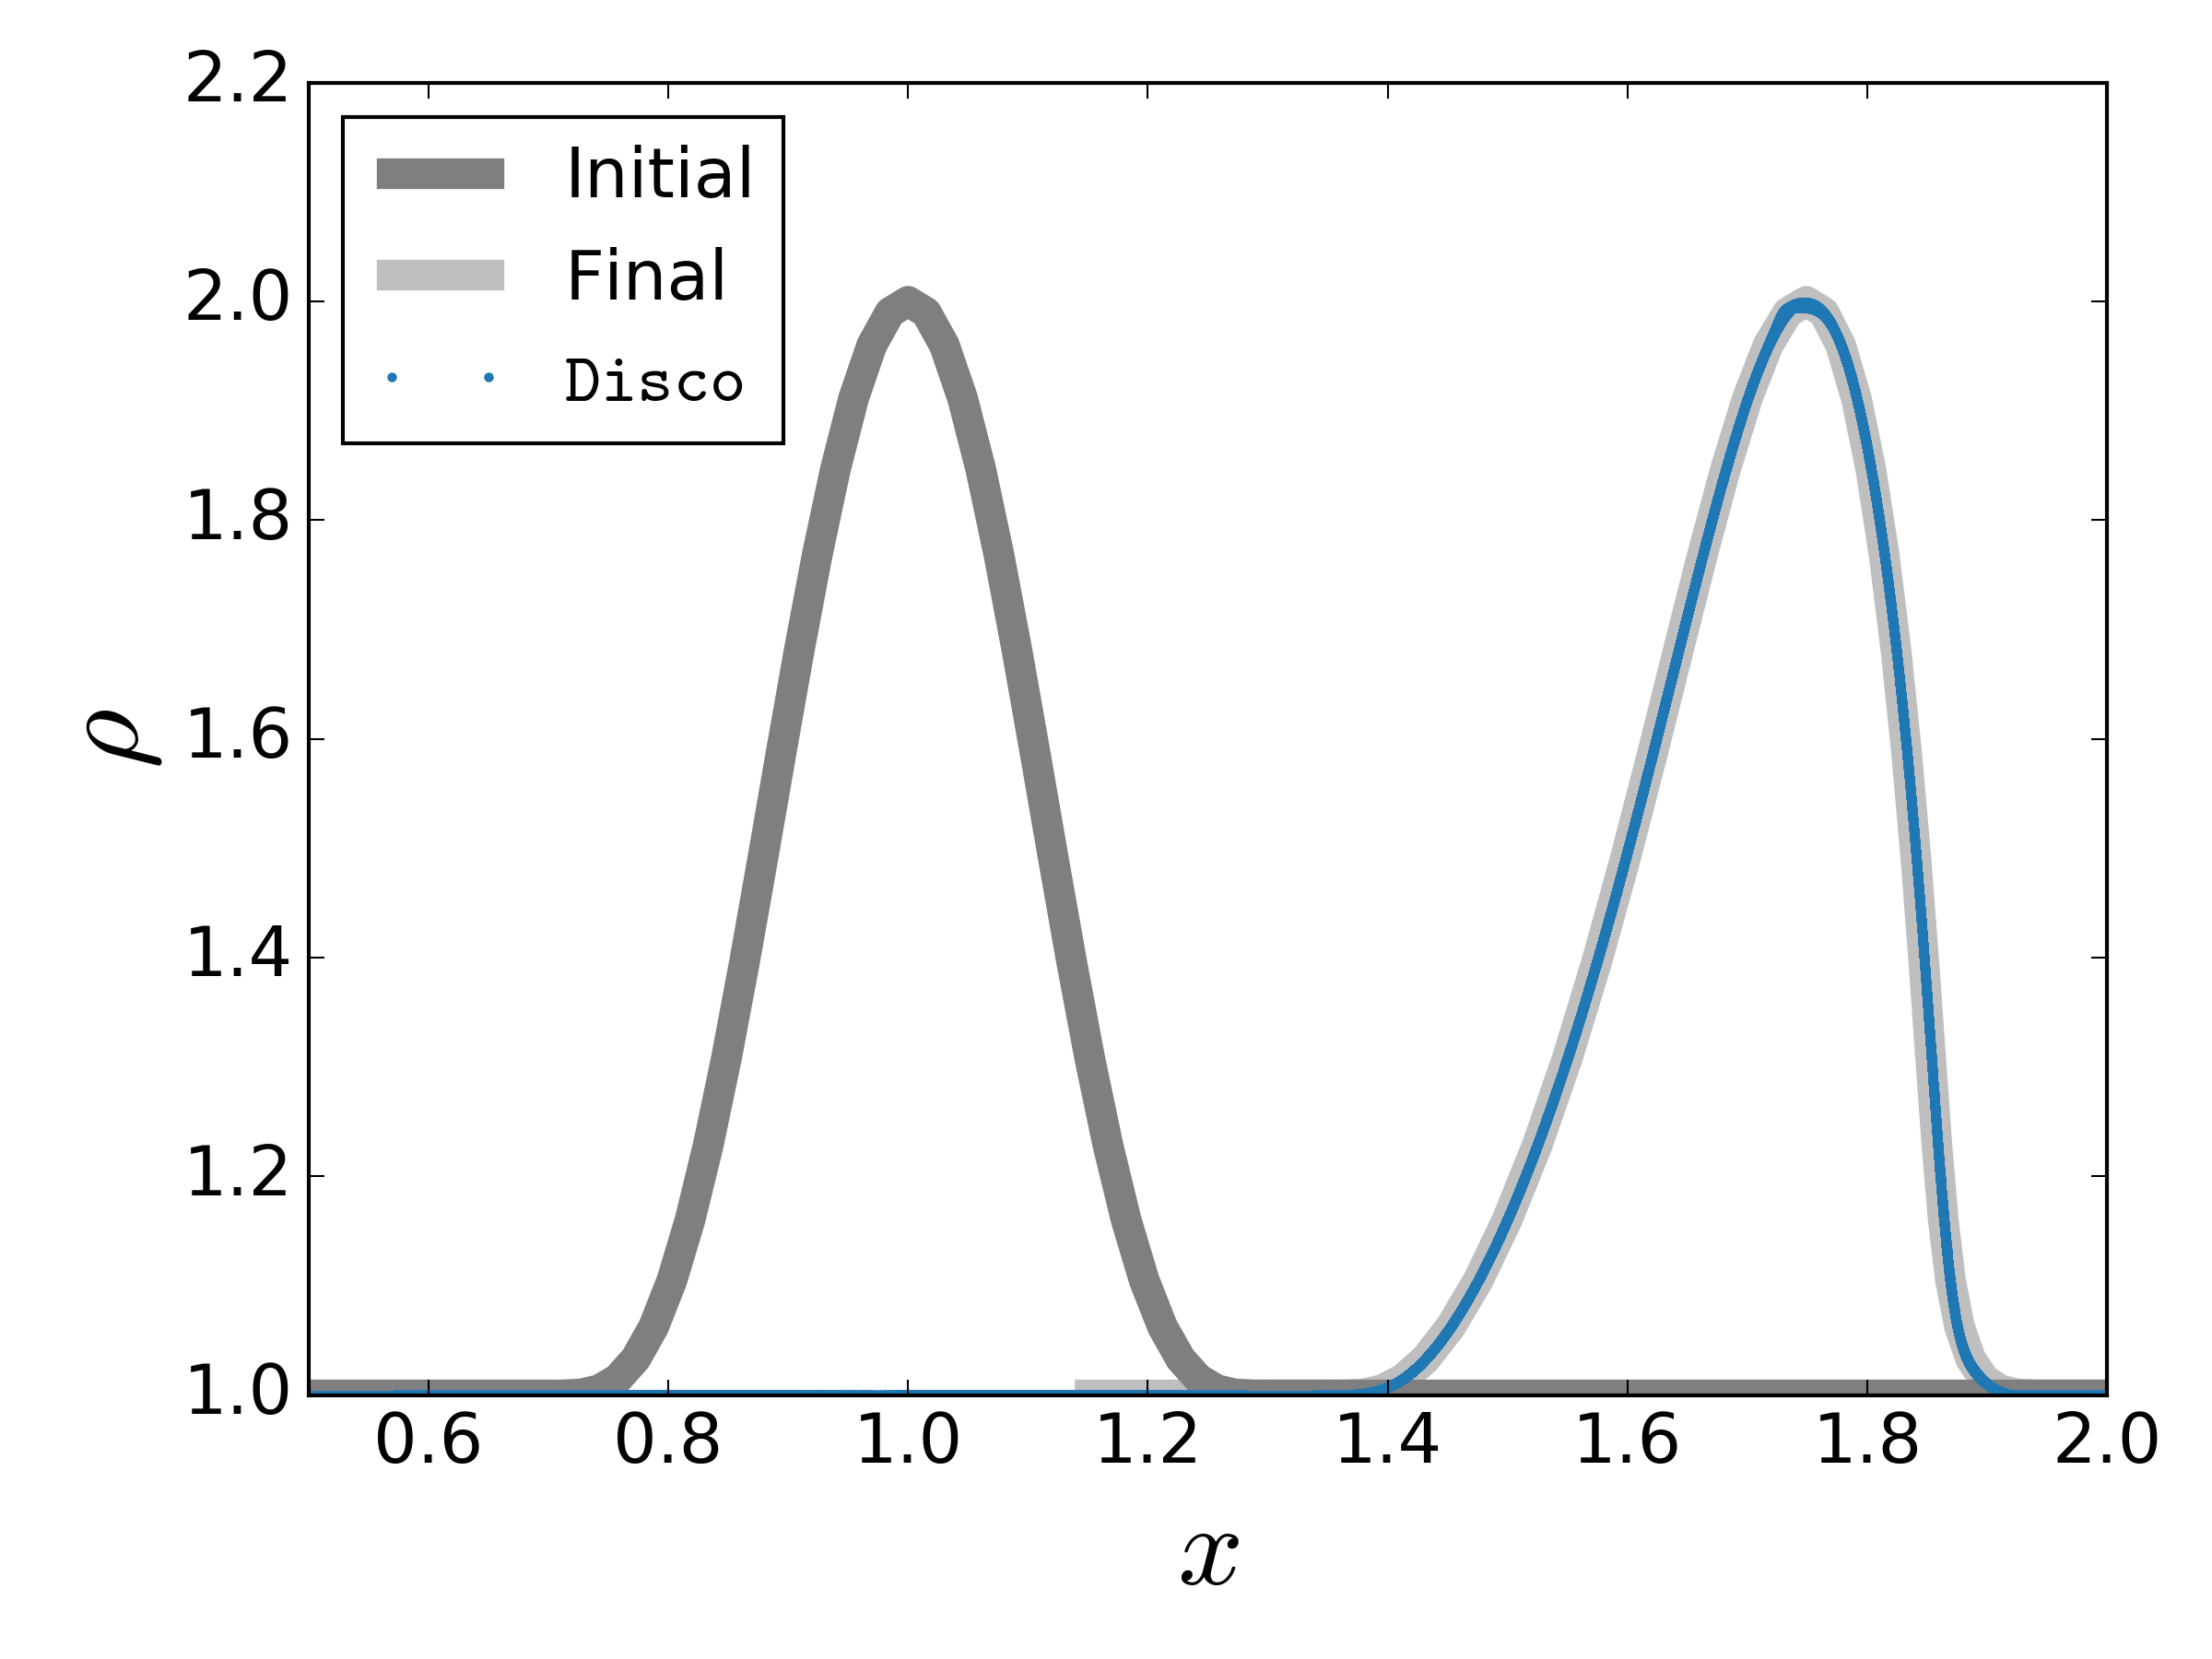
\includegraphics[width=0.65\textwidth]{figures/numerics/isen_1024.png}
\end{center}
\caption{Isentropic wave density $\rho(x)$ at $t=0.8$ for $N_r=1024$ (blue dots), exact solution (grey line), and initial condition (black line).  Despite running obliquely over the cylindrical grid, the wave maintains plane symmetry and matches the exact solution. \figlabel{isen:comp}}
\end{figure}
\begin{figure}
\begin{center}
	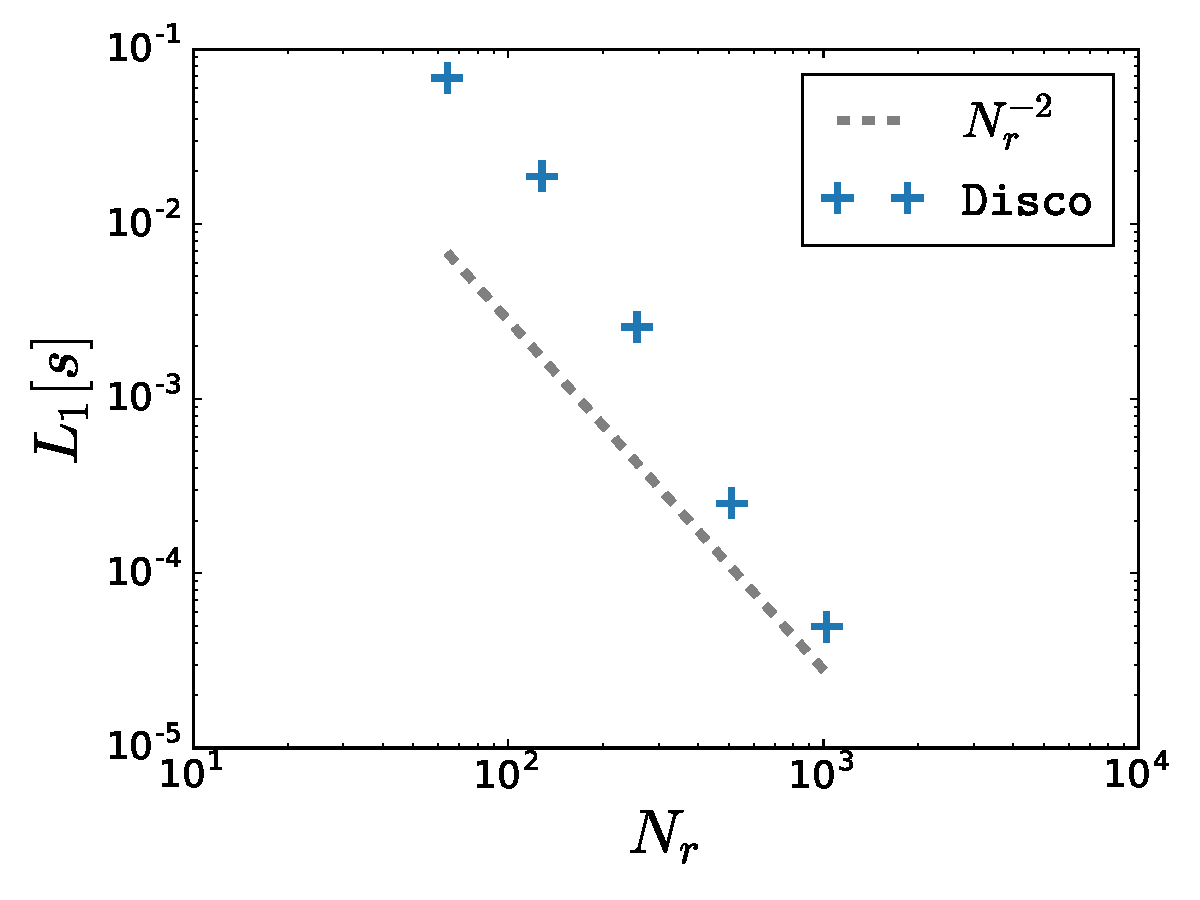
\includegraphics[width=0.65\textwidth]{figures/numerics/isen_conv.pdf}
\end{center}
\caption{$L_1$ error in the entropy $s$ as a function of $N_r$ for the isentropic wave.  The grey dashed line is a visual reference showing the expected convergence rate $N^{-2}_r$.  \figlabel{isen:conv}}
\end{figure}

\fig{isen:comp} shows density at the final time compared with the exact solution.  The agreement with the exact solution is quite good and the lack of dispersion in the data indicates that planar symmetry has been maintained.  To quantify the discrepancy we calculate the $L_1$ error of the entropy:
\begin{equation}
	L_1[s] = \sum_i |s(x_i)-s_0| \Delta A_i\ ,
\end{equation}
where $s(x_i)$ is the entropy of cell $i$, $s_0$ is the ambient (uniform) entropy, $\Delta A_i$ is the area of cell $i$ and the sum is over cells contained in the comparison box.  \fig{isen:conv} plots $L_1[s]$ versus $N_r$ and clearly shows the expected second order convergence.

\subsection{Keplerian Orbit and Inflow}
\sectlabel{test:kep}

This test checks the behaviour of thin accreting disks within the ISCO and demonstrates the efficacy of the energy variable $\tau_U$.  The initial condition is a uniform density disk $\rho(r)=\rho_0$ with uniform pressure $P(r) = P_0 \ll \rho_0$ in the Schwarzschild metric.  The velocity field $u^\mu(r)$ is equal to the geodesic velocity field $U^\mu_{geo}$ defined in \eq{Ugeo}: Keplerian outside the ISCO and smoothly plunging inside.  Outside the ISCO the gas is in a steady state.  Within this ISCO the gas should plunge according to $u^\mu(r)$, which should remain constant so long as $P \ll \rho$.

The analytic solution is given by an advection problem with non-uniform velocity profile.  Define $V = U^r / U^0$ and $F = r \rho V$. Then the continuity equation becomes:
\begin{equation}
	\frac{1}{V}\partial_t F + \partial_r F = 0\ . \eqlabel{kep:adveq}
\end{equation}
For $r > \Risco$ the velocity $V=0$ and $F(r,t)$ is a constant.  For $r < \Risco$ the solution for $F$ is:
\begin{align}
	F(r,t) &= F(r_0, 0)\ , \\
	\text{where } t &= -\int_r^{r_0} \frac{dr}{V(r)}\ .
\end{align}
This gives the solution for $\rho$ and $P$:
\begin{align}
	\rho(r,t) = \frac{r_0 V(r_0)}{r V(r)} \rho_0 \ , \\
	P(r,t) = P_0 \left(\frac{\rho(r,t)}{\rho_0}\right)^\Gam\ .
\end{align}
This one dimensional problem was run with $\rho_0 = 1.0$ and $P_0 = 10^{-4}$ on the domain $r\in[1.5M, 12M]$ in Kerr-Schild coordinates for $\Delta t = 96.344M$, where $M$ is the mass of the black hole.  This time span corresponds to a single orbit at $\Risco = 6M$.  The outer boundary was fixed, and the inner boundary was a hybrid boundary condition with $u^\mu = U^\mu_{geo}$ and $\rho$ and $P$ set to ensure isentropic infall with constant $\dot{M} \propto r\rho u^r$. We used the HLLC Riemann solver, a CFL number of 0.2, a PLM $\theta=1.5$, and $N_r = 384$ radial cells.

\begin{figure}
\begin{center}
	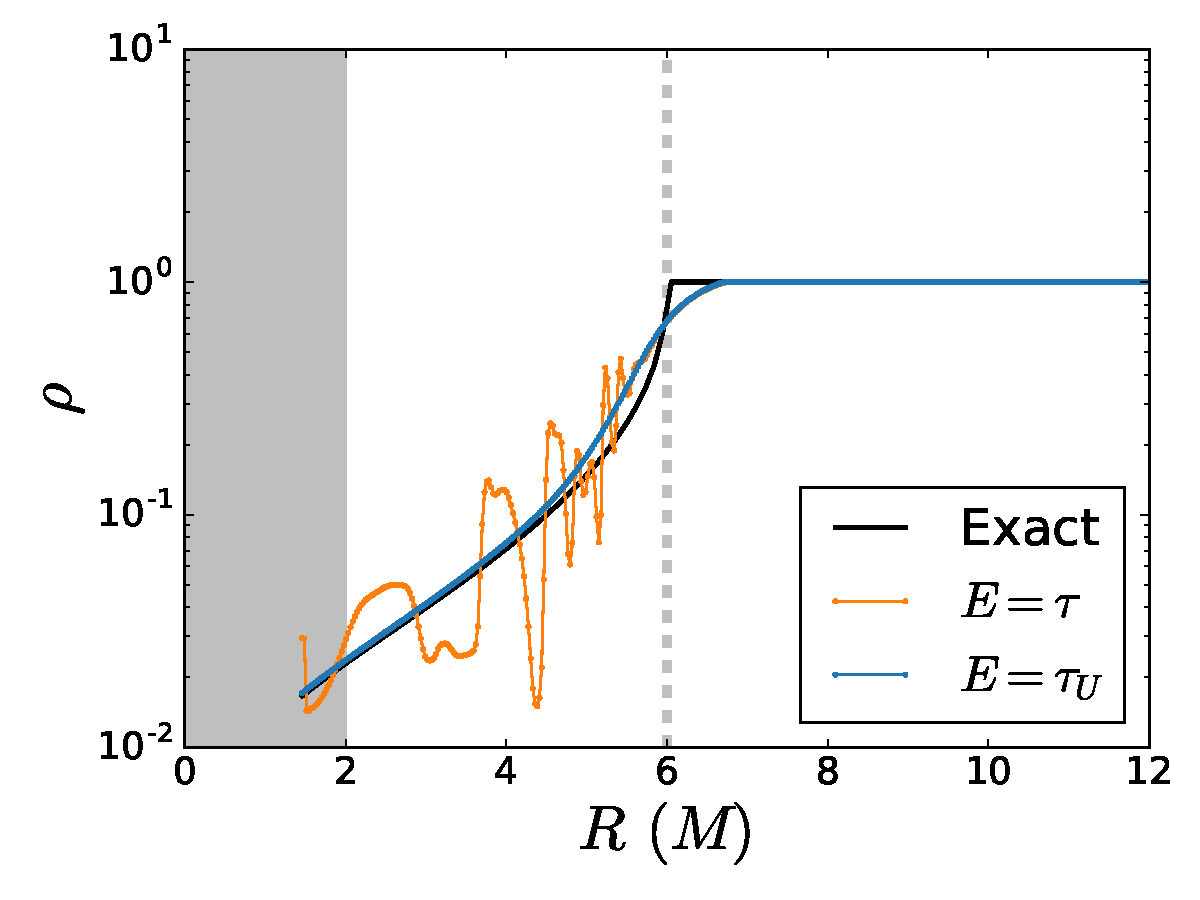
\includegraphics[width=0.6\textwidth]{figures/numerics/kep_rho.pdf}
\end{center}
\caption{Density in the Keplerian flow test at $t\approx96M$.  Exact solution in black, numerical solution with $\tau$ energy variable in orange with dots, numerical solution with $\tau_U$ energy variable in orange with dots.  The $\tau_U$ energy variable is measured in a local Keplerian frame and stably evolves the solution.  Shaded grey area is the event horizon, dashed grey line is the ISCO. \figlabel{kep:rho}}
\end{figure}

\begin{figure}
\begin{center}
	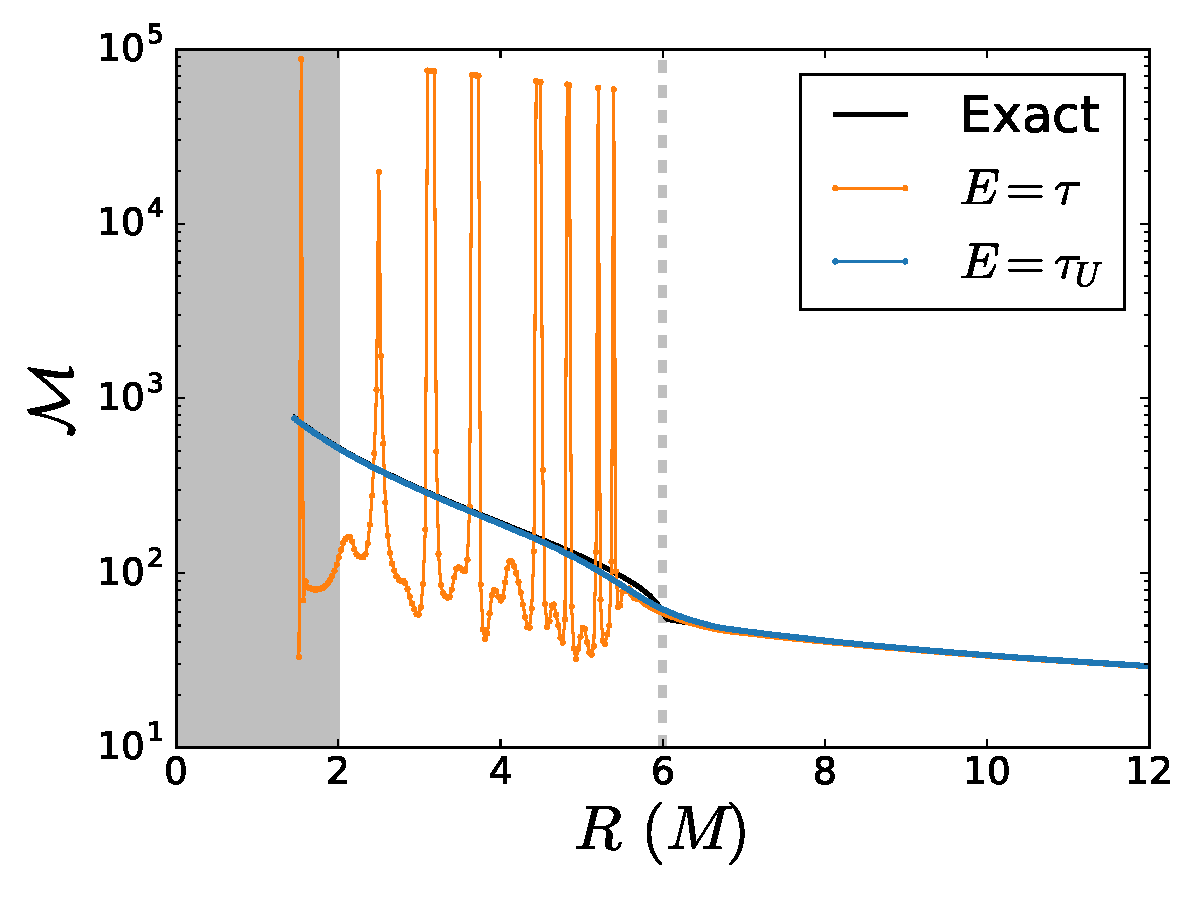
\includegraphics[width=0.6\textwidth]{figures/numerics/kep_mach.pdf}
\end{center}
\caption{Mach number $\mathcal{M} = |u|/c_s$ in the Keplerian flow test at $t\approx96M$, labelling identical to \fig{kep:rho}.   \figlabel{kep:mach}}
\end{figure}

\fig{kep:rho} and \fig{kep:mach} show density $\rho$ and Mach number $\mathcal{M} = |u|/c_s$ in the Keplerian flow test for two energy variables: the standard $\tau$ and our co-moving variable $\tau_U$ using the geodesic frame $U_{geo}$.  The Mach number of this flow is comparable to an x-ray binary or other thin sub-Eddington accretion disks.  The $\tau$ variable completely fails within the ISCO: improperly reconstructed pressures result in wild instabilities which disrupt the density.  The $\tau_U$ variable enables smooth evolution, even up to Mach numbers $\sim 10^3$ where the thermal energy is $\sim 10^{-6} = \mathcal{M}^{-2}$ of the kinetic.  The sharp cusp of the analytic solution $\Risco$ is difficult to resolve as it creates a large pressure gradient which can transport gas inwards.  Realistic disks will always have some form of angular momentum transport, so this is not an issue.

\subsection{Cartesian Shear Flow}

To test the Newtonian viscous evolution we set up a simple Cartesian shear flow with a Gaussian profile.  The Newtonian solution to the isothermal Navier-Stokes equations in this situation is:
\begin{align}
	\rho(x,t) &= \rho_0\ , \\
	P(x,t) &= P_0 \ ,\\
	v^x(x,t) &= 0 \ ,\\
	v^y(x,t) &= \frac{v_0}{\sqrt{4\pi\nu t}}\exp\left(-\frac{(x-x_0)^2}{4\nu t}\right)\ ,
\end{align}
where $\nu$ is the kinematic viscosity, $\rho_0$, $P_0$, and $v_0$ are constants, and $x_0$ is the position of the velocity peak.

To emulate this in \grdisco\ we set up a plane parallel flow on a two dimensional $r\in[1,6]$, $\phi\in[0,2\pi]$ domain with zero gradient boundary conditions on the radial boundaries.  We set $\rho_0 = 1$, $P_0=10^{-6}$, and $v_0=10^{-6}$.  The low velocity and pressure ensure Newtonian evolution.  The kinematic viscosity is $\nu=10^{-2}$, also chosen to be small so viscous heating (and the ensuing pressure gradients) will also be small.  The velocity peak is placed at $x_0 = 3$ and the evolution is from $t_0 = 0.5$ to $t_1 = 1$.  Similar to the isentropic wave, evolving this plane parallel flow across the cylindrical \disco\ grid makes this a non-trivial test as shear in both $r$ and $\phi$ will be present.  Success indicates the terms have been implemented correctly in the grid geometry.  We evolve using the HLL Riemann solver, PLM $\theta = 1.5$, and $\CFL=0.5$.  The comparison is carried out in the rectangular domain $x\in[2,4]$, $y\in[-2,2]$ which remains undisturbed by boundary fluctuations.

\begin{figure}
\begin{center}
	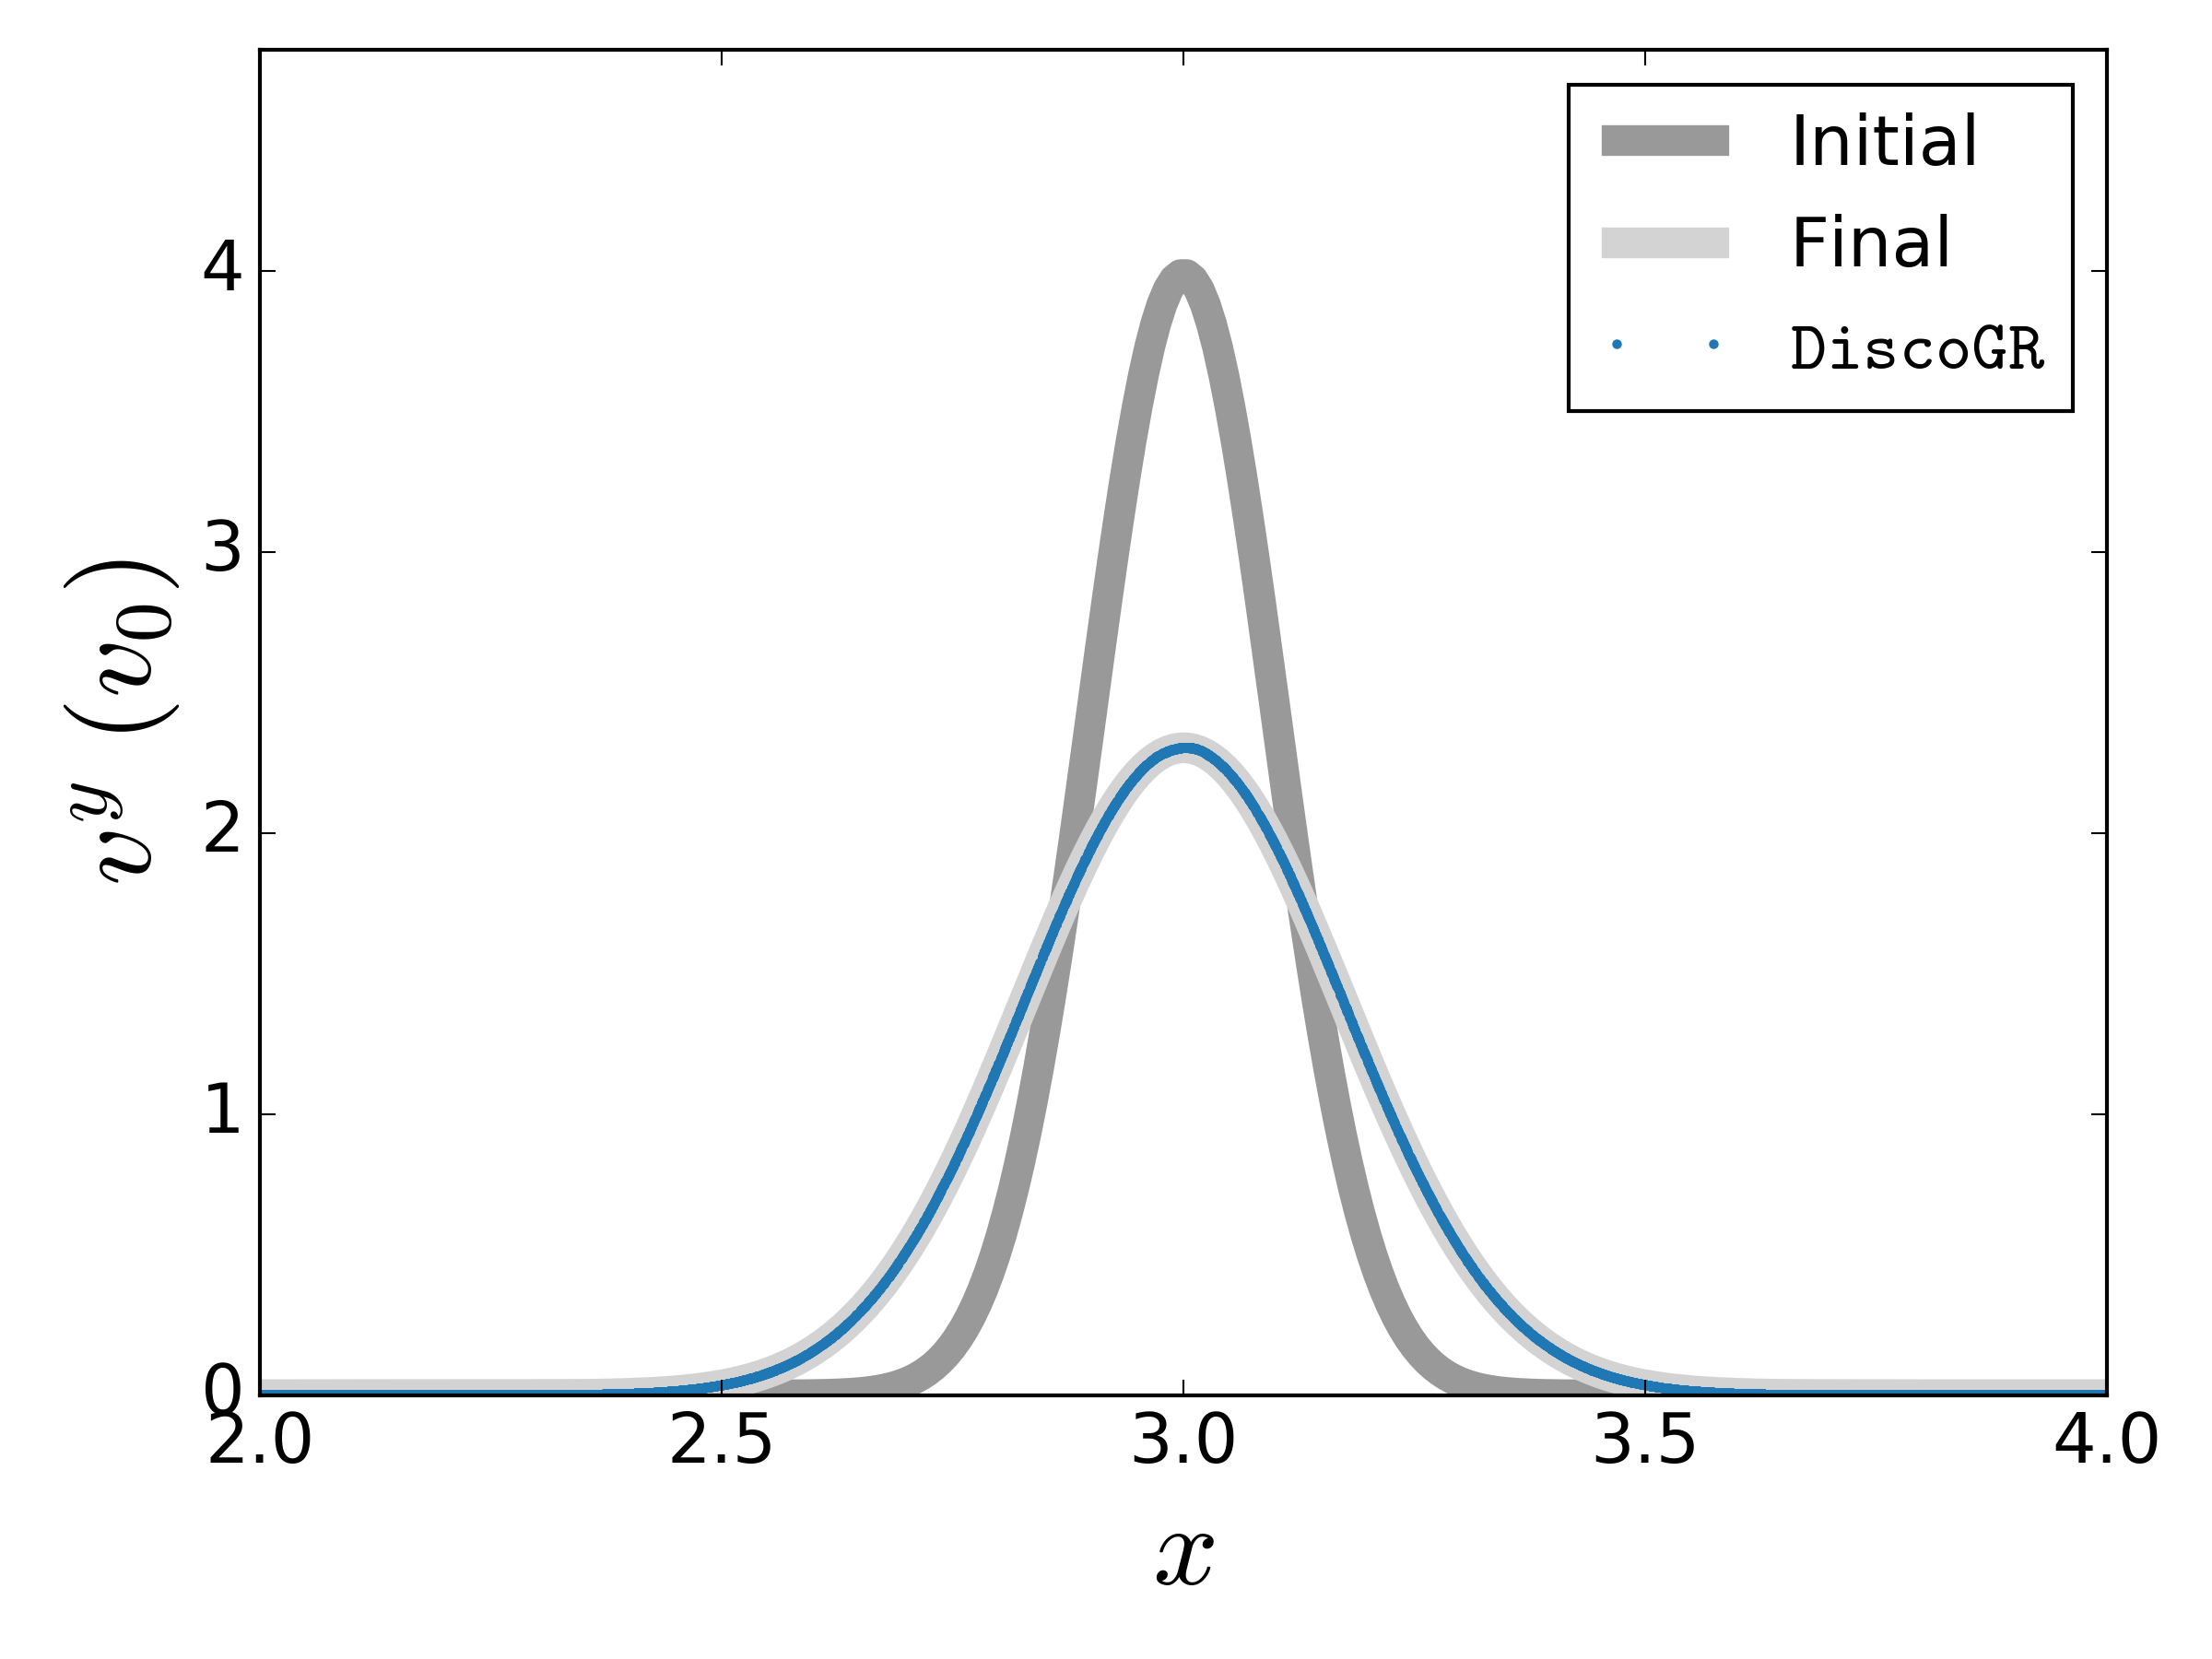
\includegraphics[width=0.6\textwidth]{figures/numerics/cs_vy.png}
\end{center}
\caption{Velocity $v^y$ in the Cartesian shear test. \grdisco\ data with $N_r=256$ at $t=1$ in blue dots, initial condition in dark grey, and final state in light grey.  \figlabel{cs:vy}}
\end{figure}

\fig{cs:vy} shows the velocity $v^y$ at the end of the calculation, compared to the initial and final states.  The agreement is very good: the error $L_1[v^y]$ is of the order $10^{-6}$, the order at which relativistic corrections affect the solution.  As with the isentropic wave, the lack of dispersion in the data indicates that planar symmetry is maintained over the curved \disco\ grid.

\subsection{Novikov--Thorne Steady State}

As a final test of \grdisco's hydrodynamics solver we find the Novikov--Thorne (NT) $\al$-disk solution in a dynamic calculation \citep{Novikov73}.  We work in the Kerr spacetime in Kerr-Schild coordinates on a radial domain $r \in [1.2M, 100M]$ with $N_r = 128$.  The Kerr parameter is $a_* =0.9$.   This domain crosses the ISCO and ergosphere and has several zones inside the event horizon.  Since the NT solution is vertically integrated and axisymmetric we work in 1D and set $N_\phi = N_z = 1$.  In this setup the density $\rho$ is actually the surface density $\Sigma = \rho H$, where $H$ is the disk scale height.  Similarly $P$ is the vertically integrated pressure.  We use $\al$-viscosity and set $\al = 0.1$.  

To balance the viscous heating we include a cooling source term corresponding to a disk blackbody with opacity due to electron scattering:
\begin{equation}
	\dot{Q} = \frac{8}{3}\frac{ \sig_{\rm SB}T^4}{\ka_{\rm es} \Sig}\ . \eqlabel{BBcooling}
\end{equation}
In \eq{BBcooling} $\sig_{\rm SB}$ is the Stefan-Boltzmann constant and $\ka_{\rm es} = 0.4$ cm\textsuperscript{2}/g is the electron scattering opacity.  This is incorporated by modifying the conservation of energy-momentum equation as:
\begin{equation}
	\nabla_\mu T^{\mu\nu} = - \dot{Q} u^\nu\ .
\end{equation}

The initial condition is the NT solution for $r>30M$ with a set accretion rate $\dot{M}$, we set $M = 10 M_\odot$ and $\dot{M} = 10^{-4} \dot{M}/y$.  Inside $30M$ the solution has uniform density and pressure.  The simulation is run for $t = 10^5 M$ with $\CFL=0.2$, PLM $\theta=1.5$, HLL Riemann solver, adiabatic index $\Gam = 5/3$, and energy frame velocity $U^\mu_{\rm geo}$. 

\begin{figure}
\begin{center}
	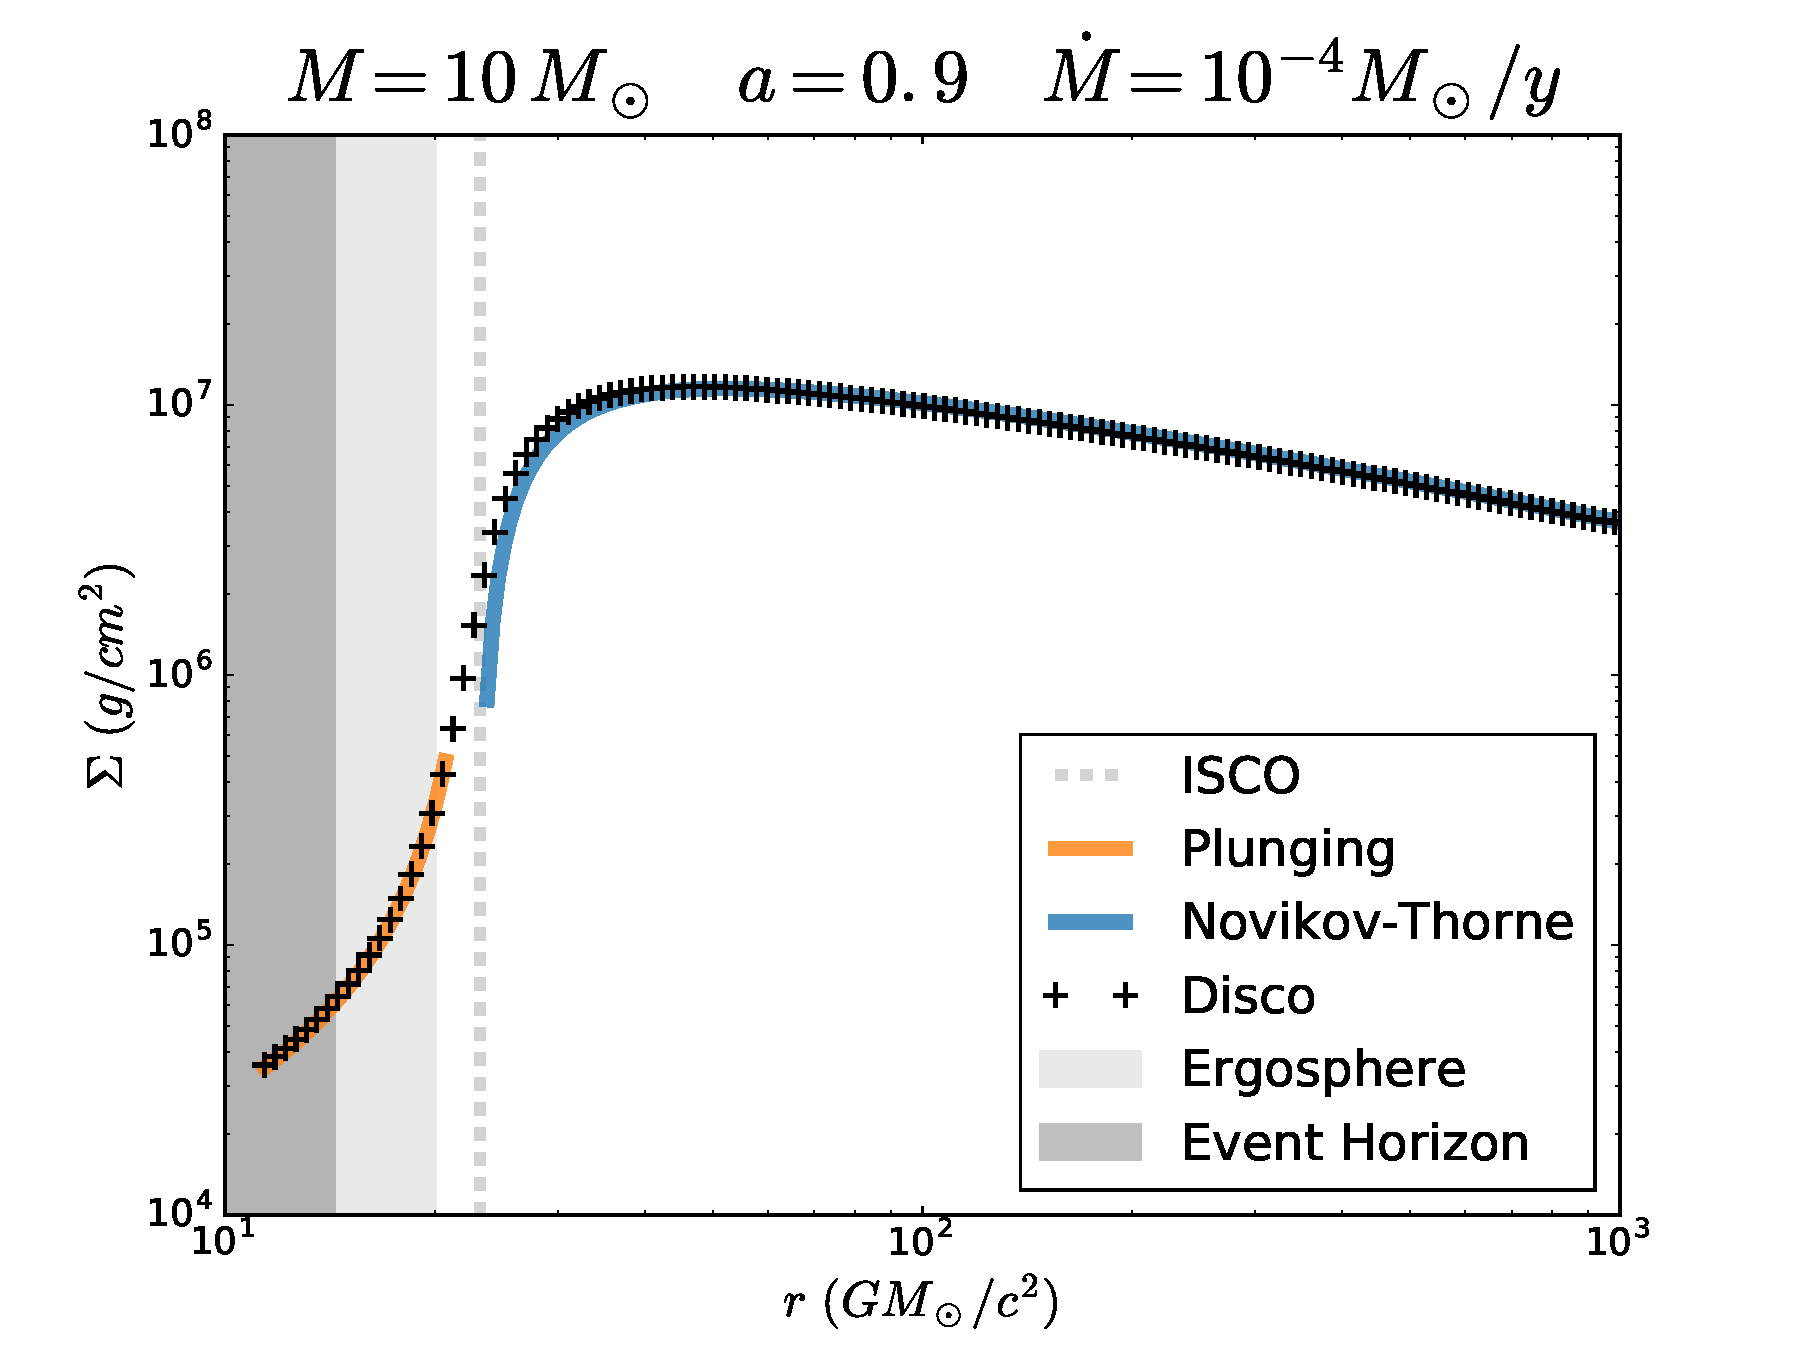
\includegraphics[width=0.65\textwidth]{figures/numerics/nt_sig.pdf}
\end{center}
\caption{Surface density in steady state with $\al$ viscosity and cooling in the Kerr metric.  Disco data in black crosses, Novikov--Thorne solution in blue, isentropic plunging in orange.  The grey dashed line denotes the ISCO, the light grey shading the ergosphere, and the dark grey the black hole interior.  \figlabel{nt:sig}}
\end{figure}

The inner disk quickly accretes as in the Keplerian inflow test, but over time is refilled due to viscous stresses.  Viscous heating is balanced by radiative cooling and a steady state is reached, shown in \fig{nt:sig}.  The density profile matches the Novikov--Thorne solution outside the ISCO and smoothly continues into the horizon.  Inside the ISCO the solution is well approximated by a ``plunging'' solution characterized by $u^\mu = U^\mu_{\rm geo}$, $\dot{M}$ constant, and $P / \Sig^\Gam$ constant.  

The NT solution by construction assumes the torque $\tau^r_\phi(r=\Risco) = 0$.  This allows for simply-parameterized algebraic solutions but causes the profile to diverge at $\Risco$.  Our dynamic calculation naturally finds a small torque at the ISCO, extending the NT solution smoothly into the horizon.

\begin{figure}
\begin{center}
	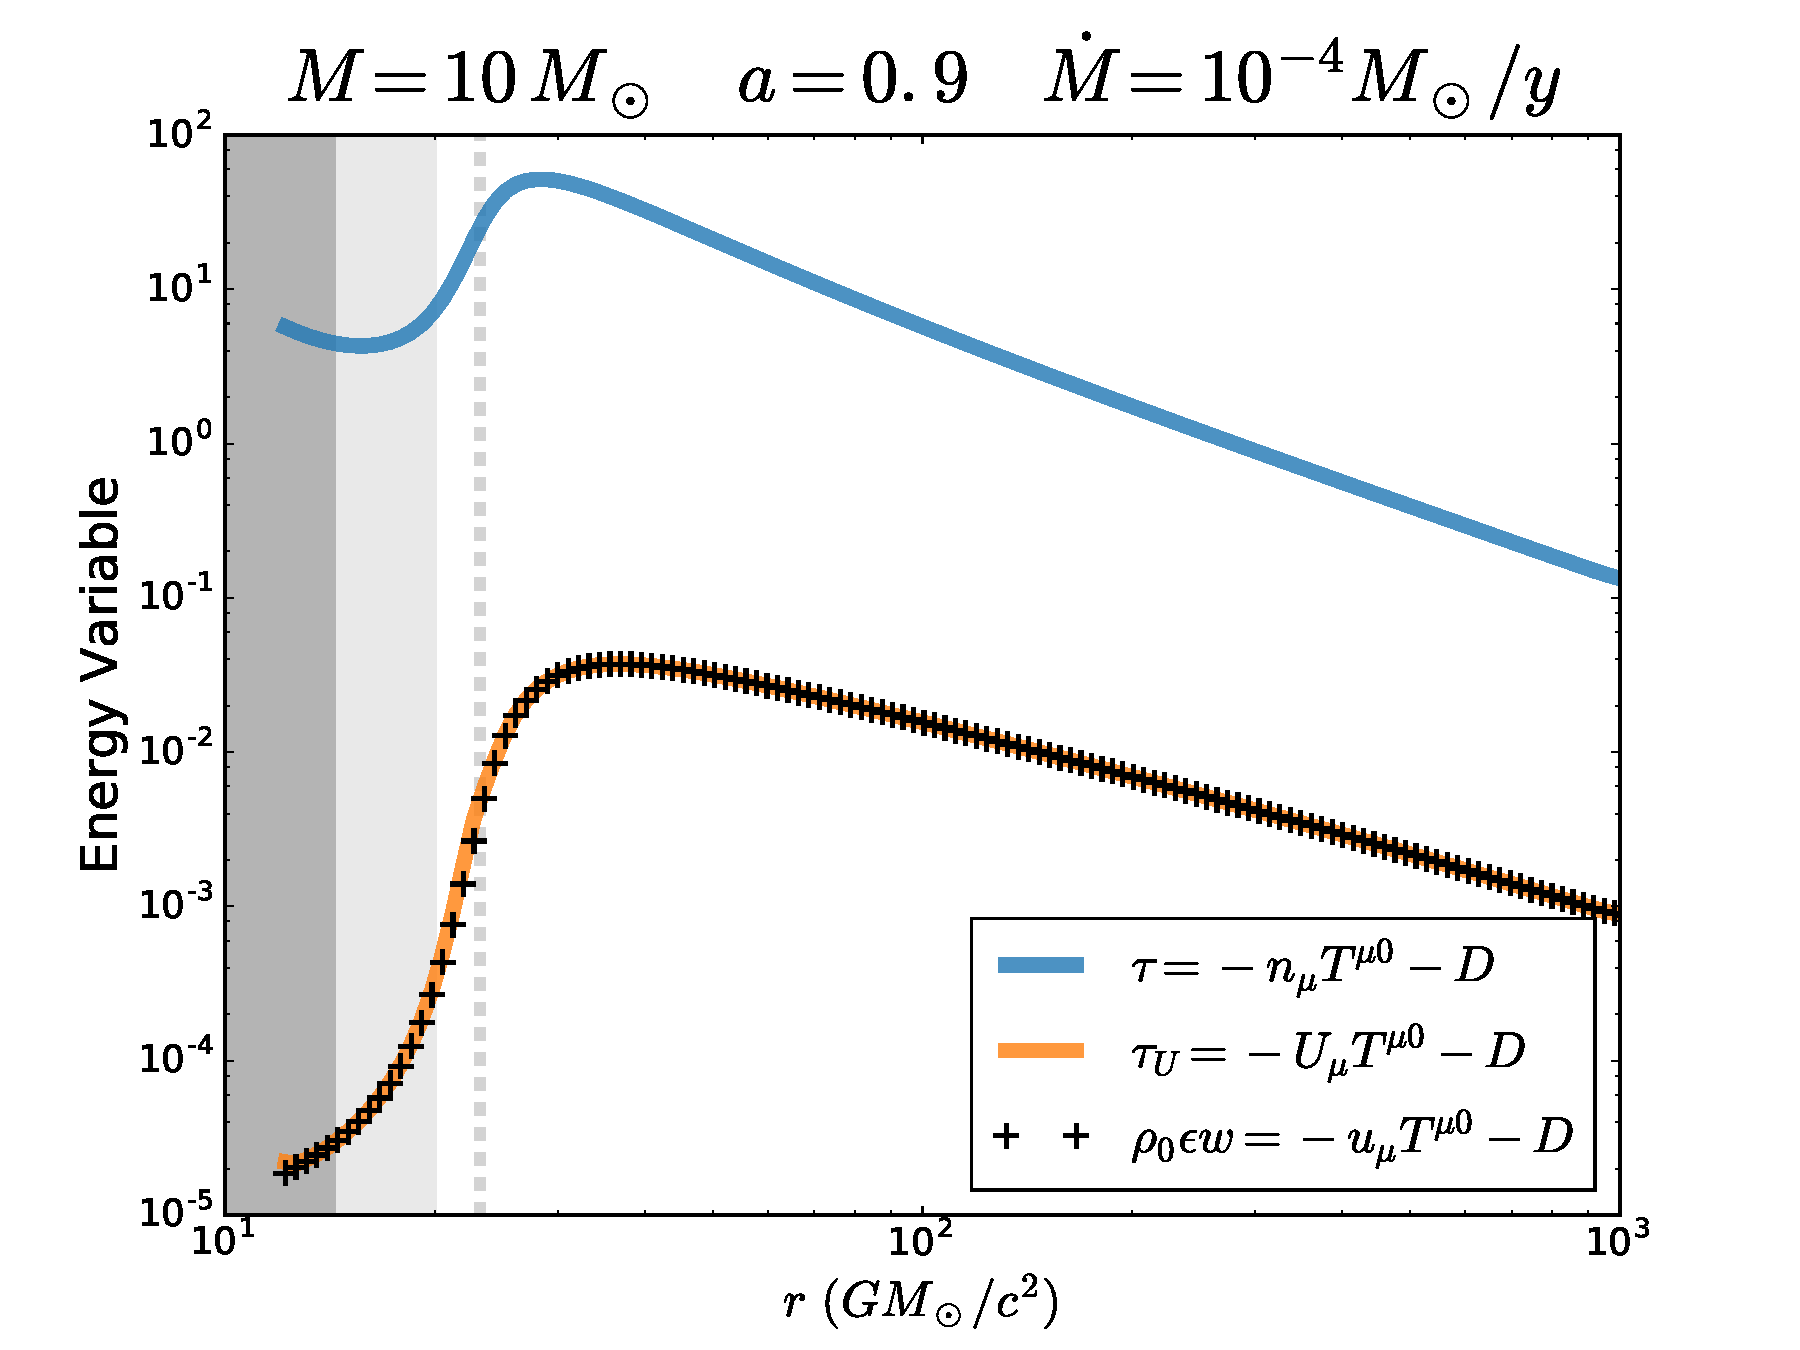
\includegraphics[width=0.65\textwidth]{figures/numerics/nt_eps.pdf}
\end{center}
\caption{Energy variables for the dynamic Novikov--Thorne solution. Standard variable $\tau$ in blue, our co-moving variable $\tau_U$ in orange, and the internal energy density in black crosses.  Other markings identical to \fig{nt:sig}.  \figlabel{nt:eps}}
\end{figure}

For illustration \fig{nt:eps} shows the energy variables $\tau$ and $\tau_U$ compared to the lab frame internal energy density $\rho \eps u^0$.  We see near agreement between the internal energy and $\tau_U$ and a vast difference with $\tau$, which is several orders of magnitude larger.  Truncation errors of the order $10^{-6}$ in the energy can easily swamp out the internal energy entirely in the inner disk.  Note that for realistic x-ray binaries the accretion rate used here is quite large.  Realistic binaries have smaller accretion rates, higher mach numbers, and would produce an even larger discrepancy between $\tau$ and the internal energy.  

%\subsection{Neutrino Dominated Accretion Flow Steady State}
\subsection{Magnetic Field Loop Advection}

The first test of \grdisco's performance in GRMHD is the advection of a magnetic field loop.  In this test the magnetic field is set to be very weak so its motion should be purely due to advection.  This tests the constrained transport scheme and the Riemann solvers, but does not include any strong field effects.

The background solution is a rigidly rotating fluid disk in flat spacetime with angular velocity $\Omega$ on the domain $r\in[0.1,0.9]$, $\phi\in[0,2\pi]$.  The fluid is in a steady state given by:
\begin{align}
	\rho &= \rho_0 \ ,\\
	P &= \frac{\Gam-1}{\Gam}\left(\rho_0 h_0\left(1-r^2\Omega^2\right)^{-\Gam / 2(\Gam-1)} - \rho_0\right)\ ,\\
	v^r &= 0 \ ,\\
	v^\phi &= \Omega\ .
\end{align}
Define the coordinates $r' = \sqrt{(x-r_0)^2 + y^2}$ and $\psi = \tan^{-1} y/(x-r_0)$.  We impose a magnetic field in the region $r' < R_0$:
\begin{align}
	B^{\widehat{\psi}} &= B_0 \sqrt{\frac{2 r'}{R_0}} \sin^2\left(\frac{\pi r'}{R_0}\right)\ .
\end{align}
In grid coordinates:
\begin{align}
	B^r &= B^{\widehat{\psi}}\left( -\sin \psi \cos \phi + \cos \psi \sin \phi\right)\ , \\
	B^\phi &= \frac{1}{r} B^{\widehat{\psi}}\left( \sin \psi \sin \phi + \cos \psi \cos \phi\right) \ .
\end{align}
We take $\rho_0 = 1$, $P_0 = \rho_0 (h_0 - 1)(\Gam-1)/\Gam = 10^{-2}$, and $\Om=1$, so the gas has sound speed $c_s \sim 10^{-1}$ and relativistic advection velocity.  The field loop is centered at $r_0 = 0.5$ and has radius $R_0 = 0.3$.  The field strength $B_0 = 10^{-4}$, so $c_A \sim 10^{-4} \ll c_s$ and the magnetic field should be simply advected without distortion.  We run the simulation until $t = 2\pi$, at which point the field loop should have completed one full orbit.

The grid has $N_r = 64$ and $N_\phi$ chosen to keep square cells. We test evolution with both HLL and HLLD Riemann solvers with mesh motion on and off.  When mesh motion is on the cells advect with angular velocity $\Omega$.  For all runs $\Gam=5/3$, PLM $\theta =1.5$, \CFL\ is 0.5, radial boundaries are held fixed, and constrained transport is used.

\begin{figure}
\begin{center}
\begin{tabular}{cc}
	HLL \& Fixed Mesh & HLL \& Moving Mesh \\
	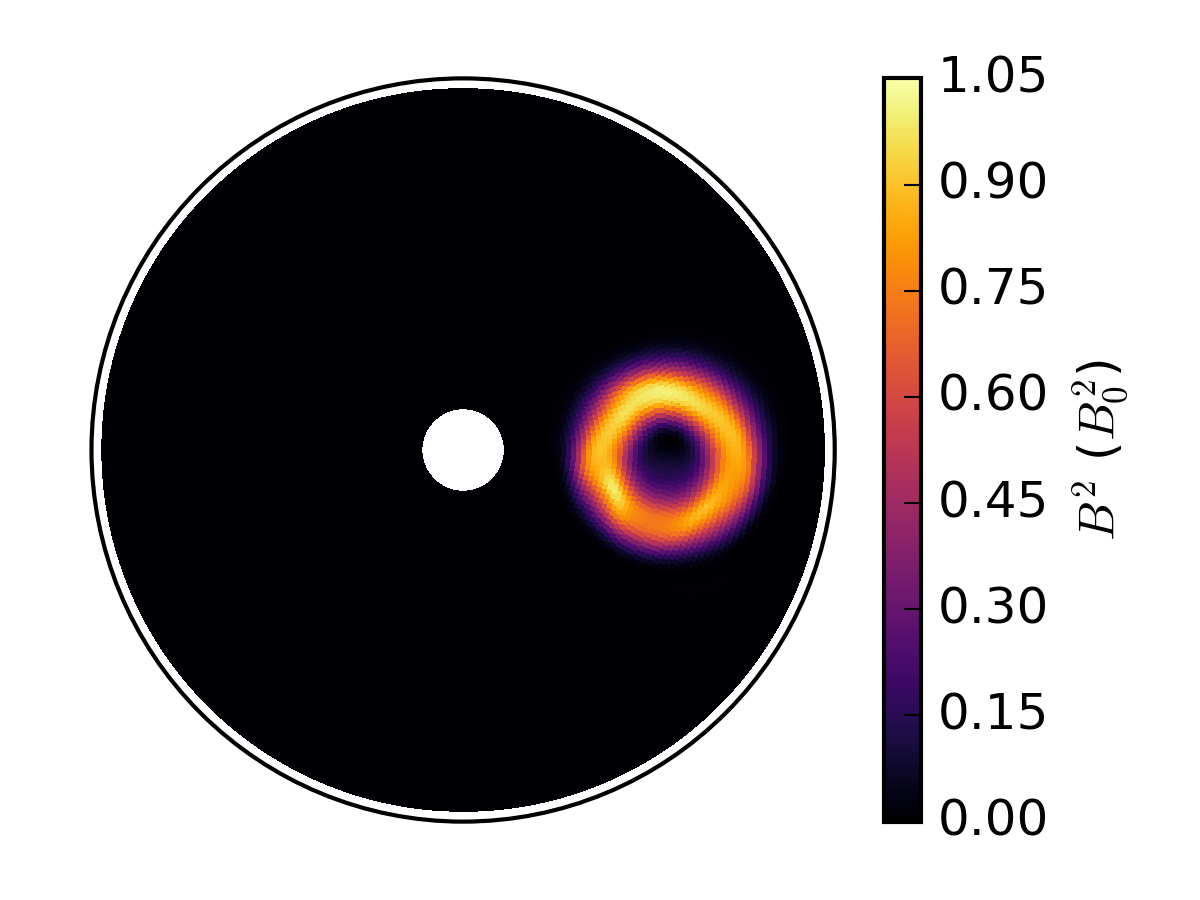
\includegraphics[width=0.5\textwidth]{figures/numerics/floop_hlle_fix.png} & 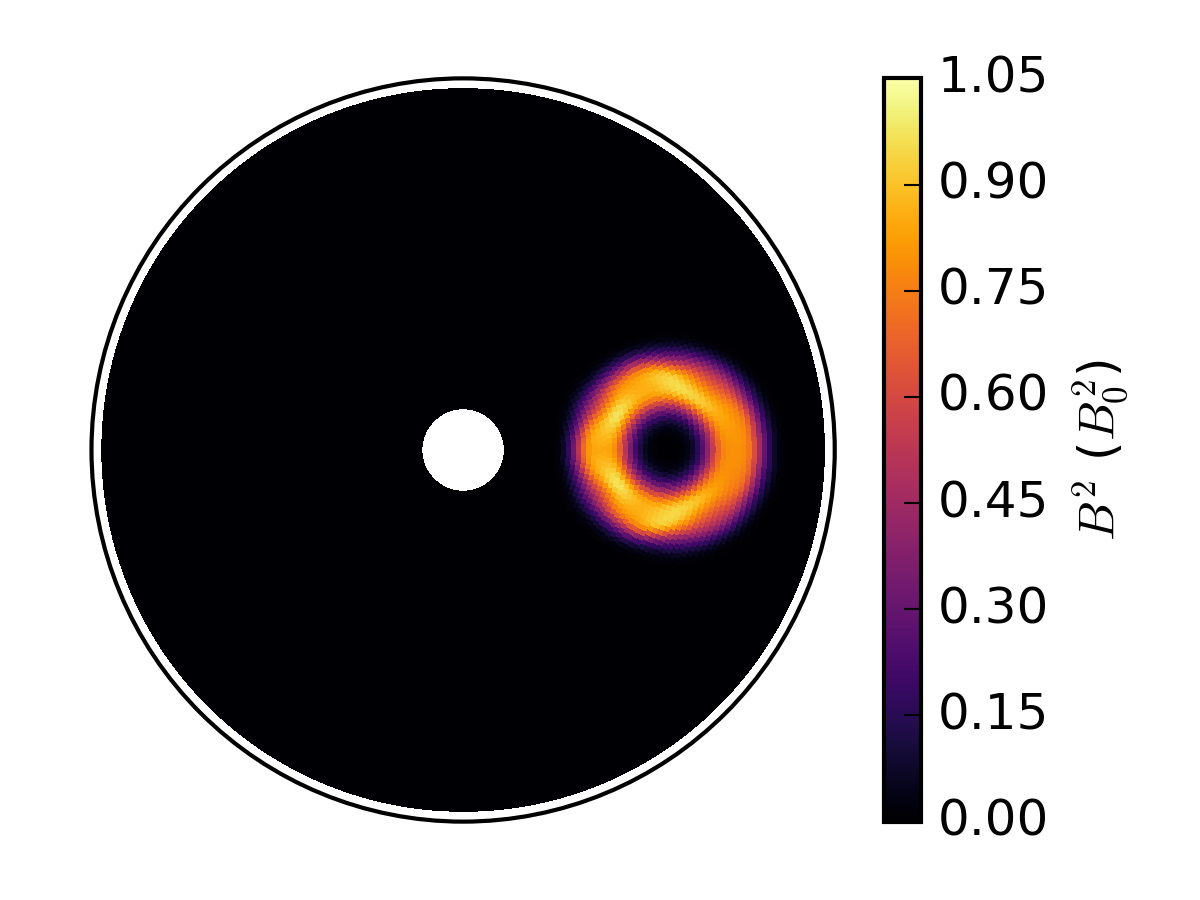
\includegraphics[width=0.5\textwidth]{figures/numerics/floop_hlle_mov.png} \\
	HLLD \& Fixed Mesh & HLLD \& Moving Mesh \\
	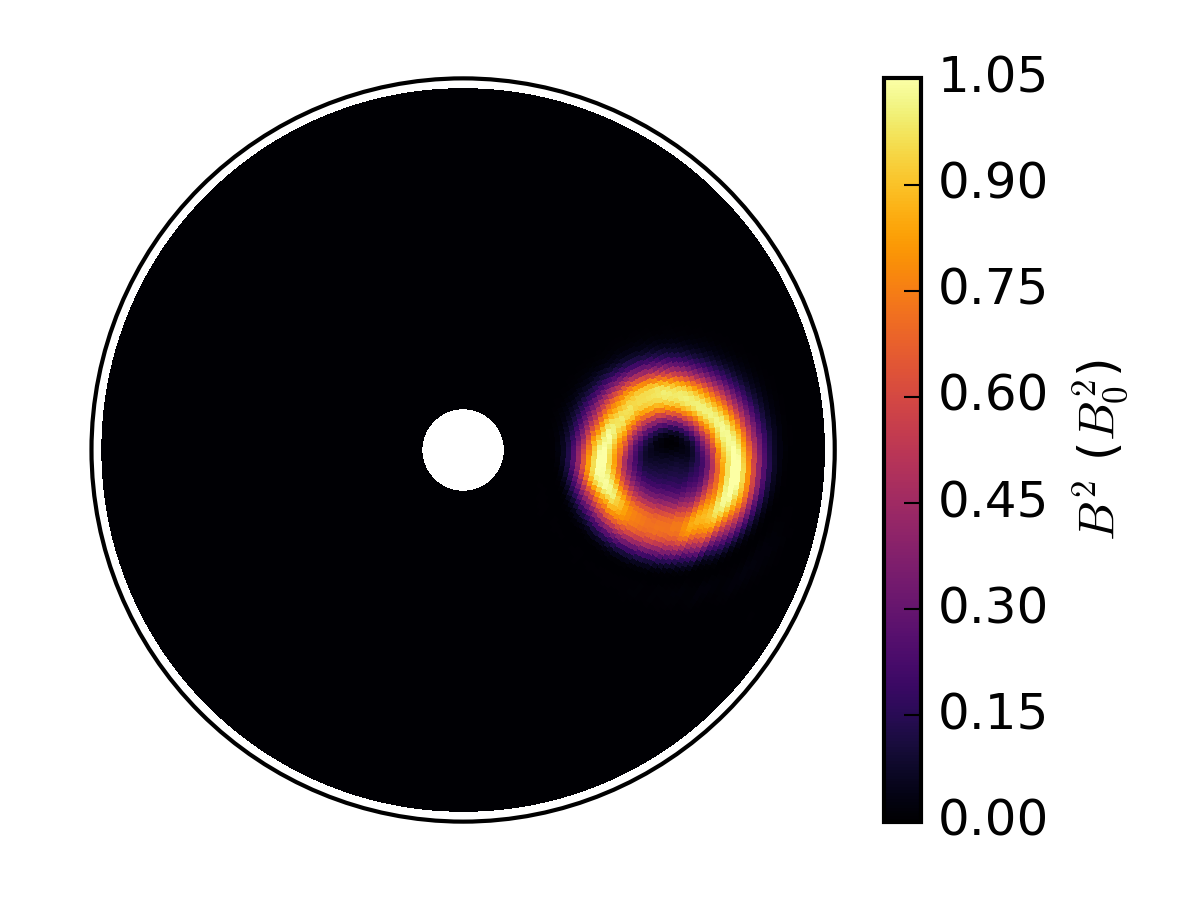
\includegraphics[width=0.5\textwidth]{figures/numerics/floop_hlld_fix.png} & 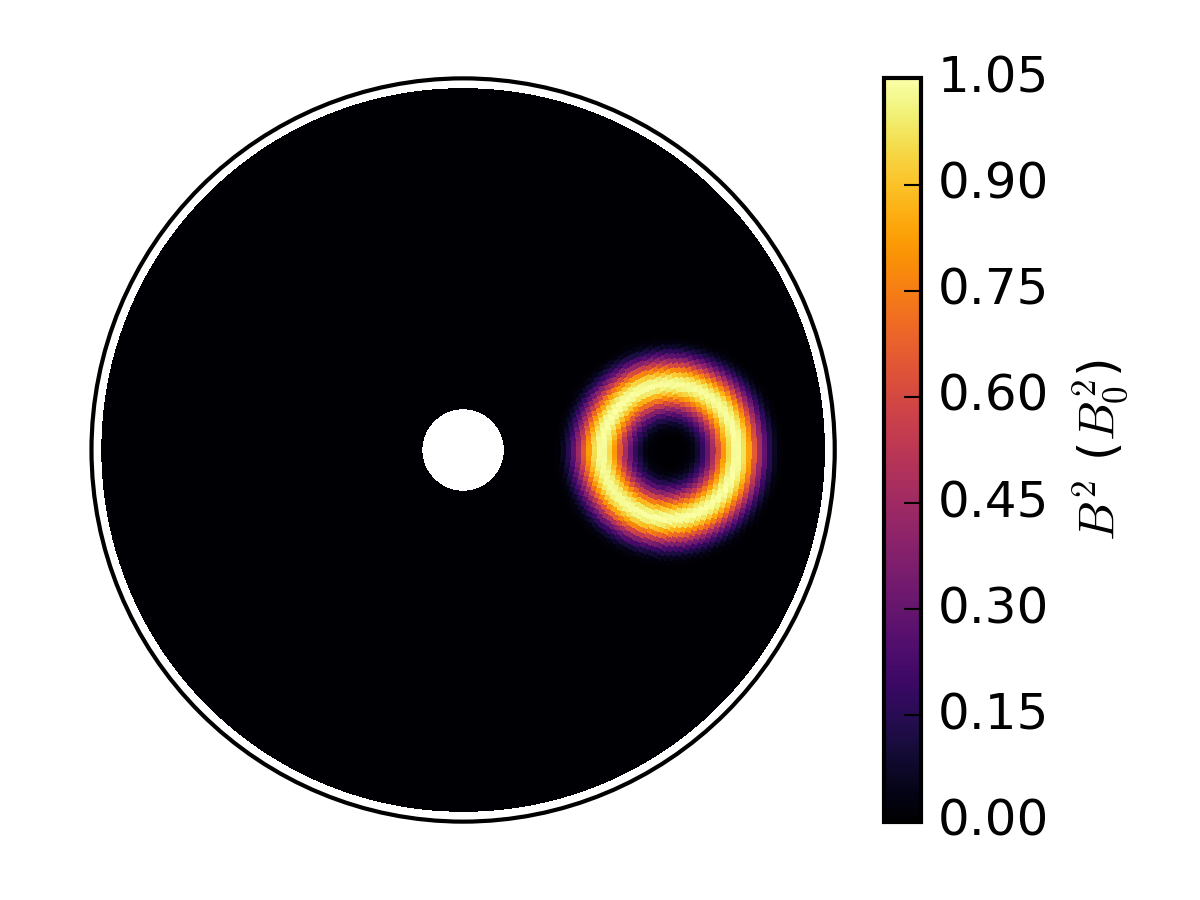
\includegraphics[width=0.5\textwidth]{figures/numerics/floop_hlld_mov.png} 
\end{tabular}
\end{center}
\caption{Lab frame magnetic field $B^2$ after one revolution in the field loop advection test.  The top row uses the HLL Riemann solver, the bottom uses HLLD.  The left column has a fixed grid while the right column uses a mesh moving at angular velocity $\Omega$.  All setups are evolved with constrained transport. The combination of HLLD with a moving mesh provides remarkable preservation of the magnetic field.  \figlabel{floop}}
\end{figure}

\fig{floop} shows the magnetic energy density $B^2$ after one orbit for all 4 runs.  With no mesh motion and HLL Riemann solver the loop develops large asymmetric fluctuations after only a single orbit.  Mesh motion symmetrizes the fluctuations but a significant discrepancy remains.  The HLLD solver does a much better job of preserving the magnetic field without dissipation, when combined with mesh motion the field loop is virtually distortion free.

%\subsection{Magnetic Blastwave}
\subsection{Linear MRI}

To test fully magnetohydrodynamic evolution we examine the linear growth of the magnetorotational instability (MRI) following the setup of \citet{Flock10}.  This is a Newtonian test, to compare with existing calculations.  

We perform the calculation in a Schwarzschild spacetime of mass $M$ in Kerr-Schild coordinates, neglecting vertical gravitational fields.  The line element is:
\begin{equation}
	ds^2 = -dt^2 + dr^2 + r^2d\phi^2 + dz^2 + \frac{2M}{r}\left(dt + dr\right)^2\ .
\end{equation}
The three dimensional domain spans $r\in[R_0, 4R_0]$, $\phi \in [0, \pi/3]$, $z\in[-R_0/2, R_0/2]$, where $R_0 = 10^6M$ to put the calculation in the Newtonian regime.  We use a grid of size $N_r = 128$, $N_z=64$, and $N_\phi$ chosen locally to keep cells cubic.  Boundary conditions are periodic in $\phi$ and $z$ and zero gradient in $r$.

The initial condition is a uniform disk of density $\rho=1$ and sound speed $c_s = 10^{-1} r \Om_K$, where $\Om_K = \sqrt{M/r^3}$ is the local Keplerian frequency. This disk then has a constant Mach number $\mathcal{M} = 10$.  The azimuthal velocity $v^\phi = \Om_K$, and the radial and vertical velocities are seeded with random noise $ v^r = \delta v^r$, $v^z=\delta v^z$, where $\delta v^i$ are uniform random numbers of with amplitude $10^{-3} \sqrt{M/R_0}$.  The magnetic field is chosen so that a particular MRI mode $n$ grows fastest, $B^z = 0.05513 n^{-1} \sqrt{M/R_0}$ and $B^r = B^\phi = 0$.  The magnetic field and velocity fluctuations are only applied between $r=2R_0$ and $r=3R_0$, otherwise both are zero.  We choose $n=4$ for this analysis.

The disk is run for 10 orbits at $R_0$ using the HLLD Riemann solver and moving the mesh with average angular velocity of each annulus.  The \CFL\ is 0.2 and the PLM $\theta=1.5$.

\begin{figure}
\begin{center}
	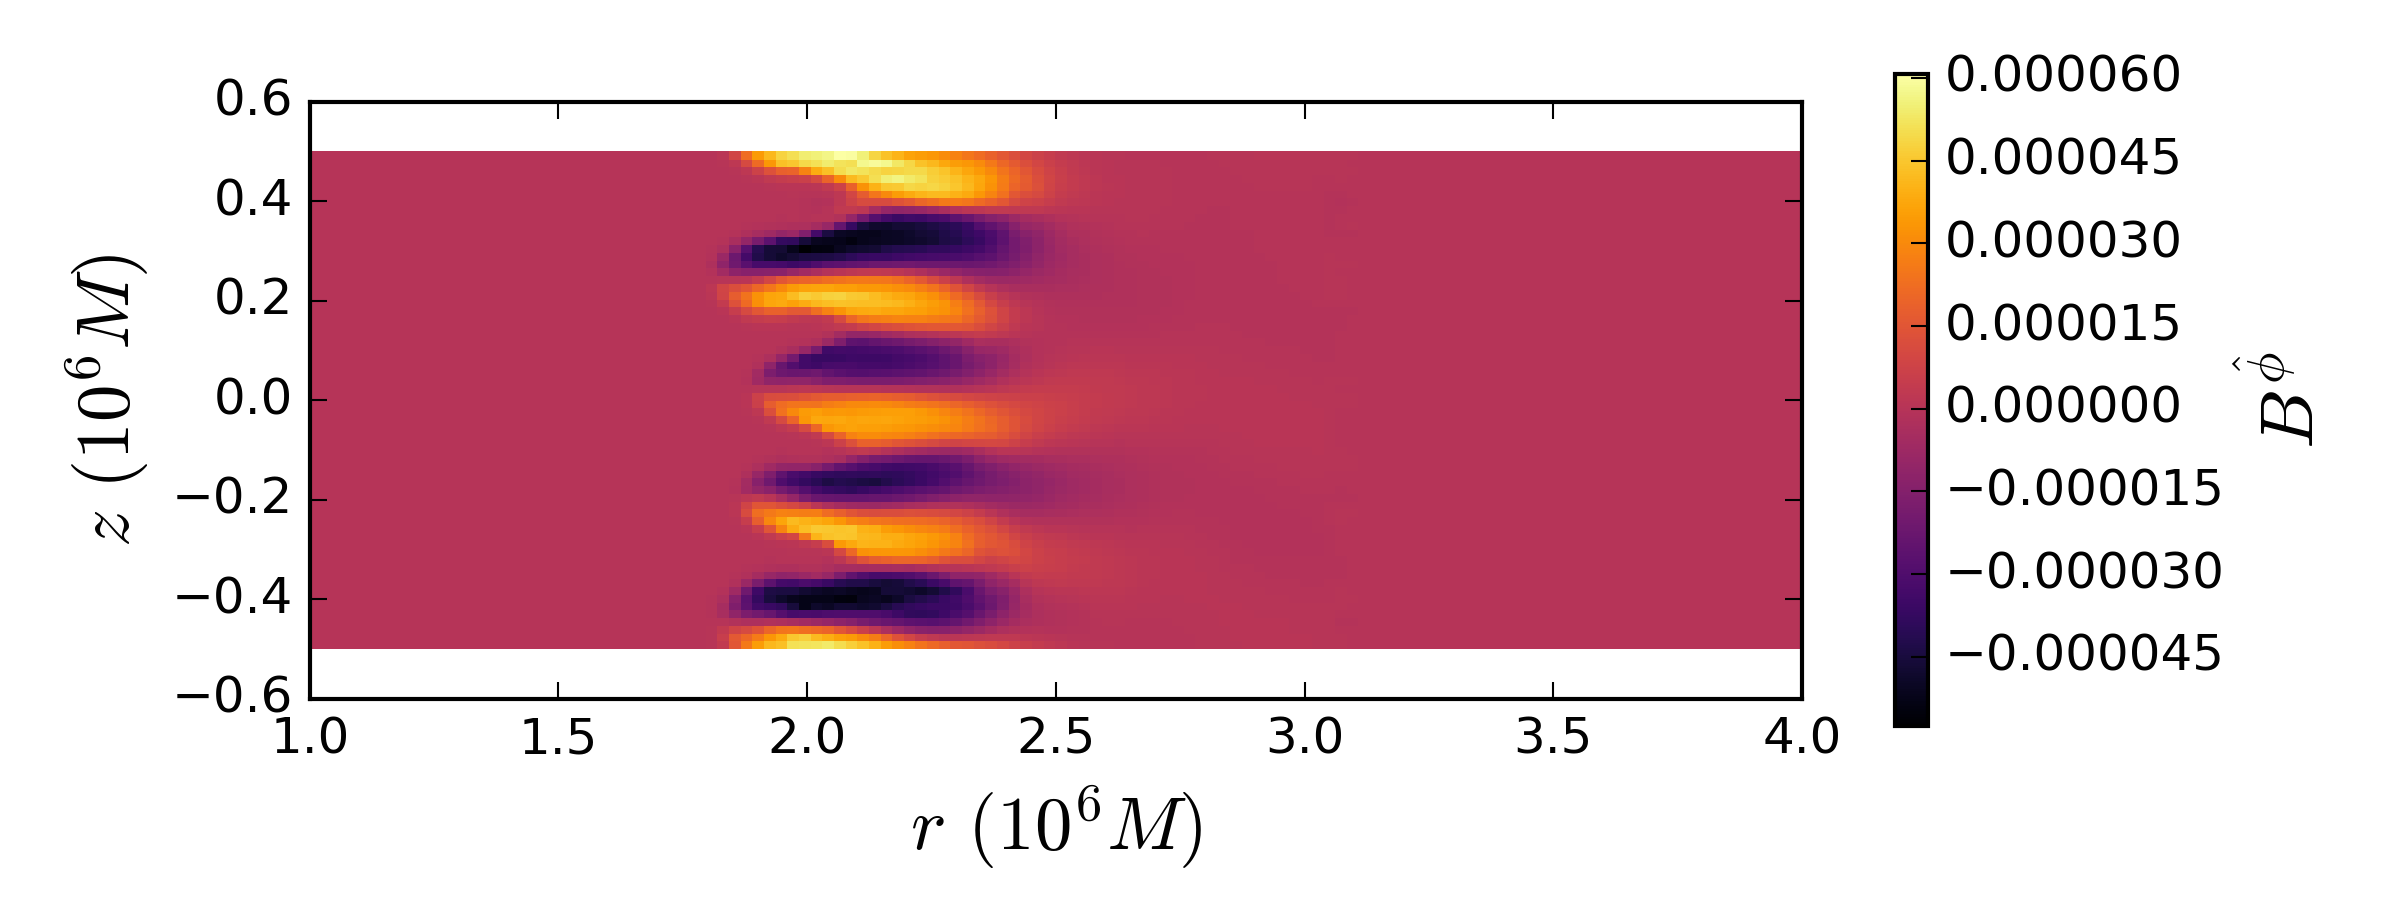
\includegraphics[width=\textwidth]{figures/numerics/flock_Bp.png}
\end{center}
\caption{Azimuthal magnetic field $B^{\hat{\phi}}$ in the linear MRI Flock test after 8 orbits at the inner radius.  The $n=4$ MRI mode has clearly been excited and is undergoing exponential growth.  This figure may be compared to Figure 5 of \citet{Flock10}. \figlabel{flock:Bp}}
\end{figure}

\fig{flock:Bp} shows the azimuthal magnetic field $B^{\hat{\phi}}$ after 8 orbits at $R_0$.  The $n=4$ mode has clearly been established and is undergoing exponential growth.  This particular variable and time was chosen to allow visual comparison with \citet{Flock10} (Figure 5).  We see a very symmetric and clean set of modes, similar to the result of their upwinded constrained transport calculation.  The amplitude of the magnetic field is also in agreement, once the $\sqrt{M/R_0}$ scaling factor is taken into account.

\begin{figure}
\begin{center}
	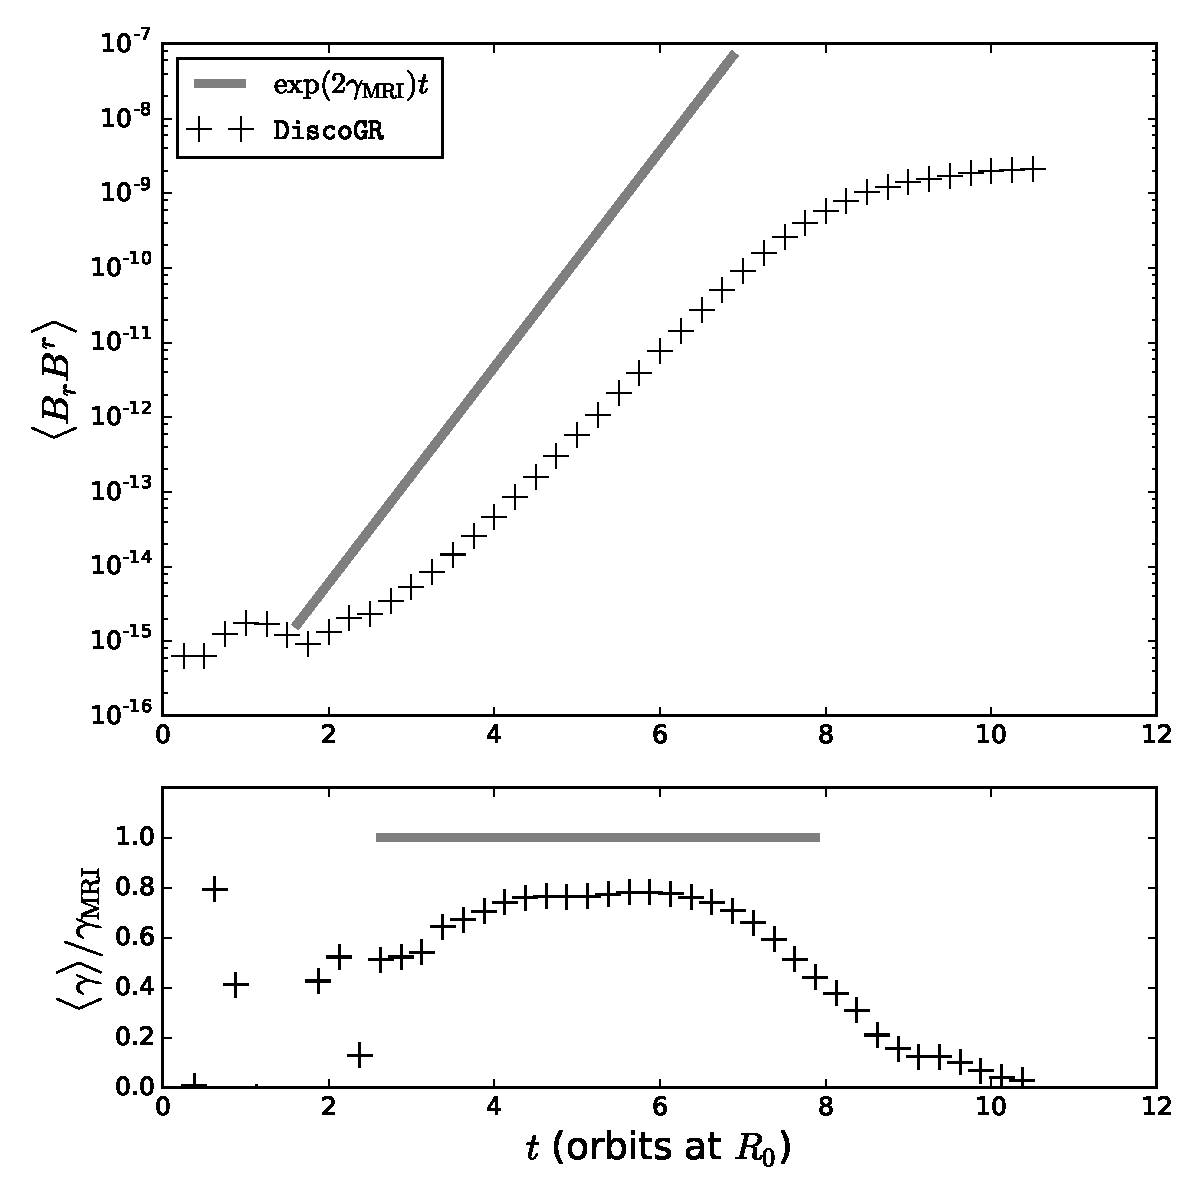
\includegraphics[width=0.8\textwidth]{figures/numerics/flock_Br2.pdf}
\end{center}
\caption{\emph{Top panel:} Growth of average radial magnetic field energy $\langle B_r B^r\rangle$ in the linear MRI Flock test.  Disco data is in black crosses and the analytic prediction in grey with arbitrary normalization.  The magnetic energy grows at an exponential rate before approaching saturation, slightly slower than the analytic prediction. \emph{Bottom panel:} Numerical growth rate $\langle \gamma \rangle$, calculated as the numerical derivative of the top panel data. The \grdisco\ growth rate reaches a maximum of $0.8 \gamma_{\rm MRI}$.  \figlabel{flock:Br2}}
\end{figure}

The quantitative test is the calculation of the effective MRI growth rate $\langle \gamma \rangle$.  \citet{Flock10} give the ideal growth rate of the magnetic field, $B = B_0 \exp(\gamma_{\rm MRI} t)$, as $\gamma_{\rm MRI} = 0.75 \Omega$.  This should be an upper bound on the growth rate for any physical or numerical MRI development.

 In the upper panel of \fig{flock:Br2} we plot the average radial magnetic energy $\langle B_r B^r\rangle$ from \grdisco\ at a cadence of one orbit.  For comparison we also plot the ideal energy growth rate $\exp(2 \gamma_{\rm MRI} t)$, using $\Omega = \Omega(r=2R_0)$ as this is the location of largest magnetic field growth.  We find as expected exponential growth of $\langle B_r B^r\rangle$ before saturation begins, but with a slightly smaller growth rate than the ideal prediction.  In the lower panel we give our numerical growth rate $\langle \gamma \rangle$, calculated as one half the numerical derivative of $\log \langle B_r B^r\rangle$ with respect to time.  After an initial transient the growth rate increases and reaches a maximum of $\sim 0.8 \gamma_{\rm MRI}$.  Although somewhat smaller than the numerical growth rates seen in \citet{Flock10}, this is in agreement with \citet{Duffell16}.

Development of GRMHD in \grdisco\ is ongoing. The results shown here show great promise for the incorporation of GRMHD into a moving mesh framework and demonstrate the robustness of moving mesh GRHD.

%%%%%%
% Summary %
%%%%%%

\section{Summary}
\sectlabel{summary}

We have introduced \grdisco, a new three dimensional GRMHD code that utiliizes a moving, shearing mesh.  The mesh motion greatly lowers the numerical dissipation while allowing for significantly longer time steps.  We have demonstrated \grdisco's performance on a number of test problems, emphasizing its performance on supersonic orbiting flows and its ability to dynamically capture steady thin accretion disks.  The MHD development of \grdisco\ is ongoing and shows great promise.  \grdisco is massively parallel and available freely online at \url{https://github.com/geoffryan/Disco.git}.

\section{Chapter Acknowledgements} \sectlabel{acknowledgements}

Computations were carried out using the Pleiades cluster at NASA Ames and on the Ria cluster at the Center for Cosmology and Particle Physics at New York University. We thank Brian Farris for many fruitful conversations and his work on Newtonian \disco.


\renewcommand{\chapid}{minidisk}

% Chapter specific commands:
\newcommand{\model}[1]{{Model \texttt{#1}}}

% Math:

\newcommand{\ave}[1]{\left \langle #1 \right \rangle}
\newcommand{\avet}[1]{ \langle #1 \rangle}
\newcommand{\aveRe}[1]{\left \langle #1 \right \rangle_\text{Re}}
\newcommand{\aveRet}[1]{ \langle #1  \rangle_\text{Re}}


\chapter{Minidisks in Circumbinary Black Hole Accretion\chaplabel{minidisk}}

This \paper\ is joint work with Andrew MacFadyen (NYU) published in \emph{The Astrophysical Journal} as \citet{Ryan17}.

\section{Chapter Abstract}

Newtonian simulations have demonstrated that accretion onto binary black holes produces accretion disks around each black hole (``minidisks''), fed by gas streams flowing through the circumbinary cavity from the surrounding circumbinary disk. We study the dynamics and radiation of an individual black hole minidisk using 2D hydrodynamical simulations performed with a new general relativistic version of the moving-mesh code Disco. We introduce a comoving energy variable that enables highly accurate integration of these high Mach number flows. Tidally induced spiral shock waves are excited in the disk and propagate through the innermost stable circular orbit, providing a Reynolds stress that causes efficient accretion by purely hydrodynamic means and producing a radiative signature brighter in hard X-rays than the Novikov--Thorne model. Disk cooling is provided by a local blackbody prescription that allows the disk to evolve self-consistently to a temperature profile where hydrodynamic heating is balanced by radiative cooling. We find that the spiral shock structure is in agreement with the relativistic dispersion relation for tightly wound linear waves. We measure the shock-induced dissipation and find outward angular momentum transport corresponding to an effective alpha parameter of order 0.01. We perform ray-tracing image calculations from the simulations to produce theoretical minidisk spectra and viewing-angle-dependent images for comparison with observations.

%%%%%
%Section 1 - Introduction
%%%%%

\section{Introduction} \sectlabel{intro}


Supermassive black hole binaries (SMBHBs) are expected to form after mergers of galaxies during hierarchical structure formation.  The binaries settle to the center of the merger remnant and are expected to be embedded in gas. Gaseous accretion onto black hole binaries is thus a problem of compelling interest for understanding the dynamics and radiation of merging black holes. Pulsar timing array (PTA) measurements have started to come in tension with expected rates of nanohertz gravitational wave (GW) emission from predicted populations of SMBHBs \citep{Shannon15}. This raises the question of whether SMBHBs merge at all or are driven through the PTA band by interaction with ambient gas. Electromagnetic (EM) or GW detection of an SMBHB could help answer this question but requires a detailed understanding of the complex dynamics of these systems. \cite{Graham15A} have recently claimed that a 5.2 yr periodicity detected in Catalina Real-Time Transient Survey observations of the quasar PG 1302 corresponds to a black hole binary with mass $10^{8-9}M_{\odot}$ and separation $\sim 10^{-2}$ pc \citep[see also][]{Graham15B}. 

Black hole binaries also form as the evolutionary endpoint of massive star binaries or by capture in dense stellar environments. The recent LIGO detection of GWs from stellar-mass binary black holes calls attention to the dynamics of binary evolution in this mass range. In particular, if gas is present during some phase of these systems, circumbinary accretion will occur and may effect the orbital evolution or lead to the production of an electromagnetic counterpart \citep{Bartos16, Perna16}

Analytic treatments \citep{Artymowicz94,Milos05,Shapiro10} predicted that binary black holes with sufficiently large mass ratio embedded in gas disks would reside in a circumbinary cavity of radius twice the binary separation $a$ maintained by tidal torques. It was thought that these torques prevented accretion onto the black holes. However, multidimensional numerical simulations \citep{MacFadyen08, Noble12, Farris12, DOrazio12,Gold14, Farris14, Farris15A, Farris15B,Shi15, Bankert15,Schnittman15,delValle15,Young15,DOrazio16, Munoz16,Miranda16} have demonstrated that gas streams enter the circumbinary cavity and feed accretion disks around each of the individual black holes. We term these disks ``minidisks.'' These simulations find that accretion is not significantly suppressed compared to the accretion rate expected for a single black hole with the binary mass \citep{Farris14,Shi15}.

Electromagnetic emission from the minidisk may be of importance for identifying SMBHBs through the spectral energy distribution (SED) of observed active galactic nuclei (AGNs). \cite{Roedig14} predict a notch in the SED appearing between characteristic photon energy corresponding to the circumbinary disk and the minidisks. It is therefore of importance to carefully calculate minidisk emission models as searches for SMBHBs continue \citep{Runnoe15,Li16,Charisi16}.

Due to the large dynamic range of length scales required for this problem, global simulations of these disks have been restricted to those that either excise the cavity completely or employ mass sinks with approximate accretion prescriptions.  This is necessary to prevent artificial accumulation of mass near each black hole, but it wipes out all detailed structure of the minidisks themselves.

In this work we present the results of 2D inviscid general relativistic hydrodynamic (GRHD) simulations of accretion disks around an individual member of a black hole binary. These simulations focus on the minidisks seen in global circumbinary accretion simulations and can be seen as ``zoomed-in'' simulations of the hydrodynamics in the immediate vicinity of one of the black holes.  These simulations serve a double purpose. First, they provide a much better resolved view of minidisk emission structure, helping to inform searches for EM counterparts of SMBH binaries.  Second, the detailed accretion dynamics can inform the accretion prescriptions used in large-scale Newtonian simulations, facilitating the approach to a global understanding of circumbinary accretion.

Our GRHD simulations utilize Kerr--Schild coordinates, which have the advantage that the inner edge of the grid can be extended inside the event horizon of the black hole, thus providing a physically realistic inner boundary condition. In this study we consider the case of nonrotating black holes in the Schwarzschild metric.

  We find that minidisks accrete via ideal hydrodynamical processes alone without the need for outward angular momentum transport due to the magnetorotational instability (MRI) often modelled with an $\alpha$ prescription.
This is due to the presence of spiral shocks excited by the tidal forces of the binary companion. These shocks heat the disk and provide an outward angular momentum flux. We include local 
blackbody cooling with electron-scattering opacity to remove shock-generated
heat self-consistently from the disk.  This allows the disk to find a natural
temperature equilibrium and allows a direct estimate of the SED.

The role of spiral shocks in transporting angular momentum has been a matter of discussion for many decades.  Early numerical work by \cite{Sawada86} and analytical work by \cite{Spruit87} established the general picture: tidal forces from a binary companion excite spiral density waves that carry negative angular momentum and can steepen into shocks.  The torque from spiral shocks decreases with the scale height of the disk (or equivalently with increasing disk Mach number $\mathcal{M}$) and is sensitive to the adiabatic index $\Gamma$ of the gas.  Later numerical work confirmed these trends \citep{Godon98, Blondin00}.  Recently, \cite{Rafikov16} has established the torque-shock dissipation connection under a more general framework.  \cite{Ju16} have examined accretion due to spiral shocks in cataclysmic variables (CVs) with 2D Newtonian hydrodynamics and 3D Newtonian magnetohydrodynamics, \cite{Zhu16} performed a similar analysis with blackbody cooling in circumplanetary disks, and \cite{Bae16} have investigated the stability of spiral shocks in 3D Newtonian hydrodynamics.

In environments with sufficiently hot gas or extreme mass ratio binaries, it is possible that a cavity does not form within the circumbinary disk \citep{delValle14,delValle15}. In such conditions the accretion near the black holes will have very different structure than the stream-fed minidisk picture under consideration here. This work focuses on the case where the circumbinary disk is sufficiently thin that a cavity has formed.

This paper is organized as follows: In \sect{numerics} we present the
numerical setup used in the simulations---a version of the \Disco{} code 
modified to work in an arbitrary spacetime, with optimizations for thin 
relativistic accretion disks including a carefully chosen energy variable.  In Section \sect{models} we detail the 
minidisk models calculated.  Section \sect{analysis} introduces the fiducial run and details the analysis performed.  Section \sect{results} applies the analysis to all models, shows the effect of shocks on angular momentum transport, and calculates effective $\alpha$ values and spectra. Results are discussed in Section \sect{discussion} and the work is summarized in Section \sect{summary}.


%%%%%
%Section 2 - Numerical Setup
%%%%%

\section{Numerical Setup} \sectlabel{numerics}


The basis of our hydrodynamics scheme is the \Disco{} code, a moving-mesh hydrodynamics
code optimized for disk geometry. This code was first used in the context of
protoplanetary disks \citep{Duffell12, Duffell13A, Duffell14} and later applied 
to circumbinary accretion \citep{Farris14, Farris15A, Farris15B}. 

In the present work we have extended the \Disco{} code to solve the GRHD equations in a fixed spacetime:
\begin{equation}
    \nabla_\mu \rho_0 u^\mu = 0 \text{ and } \nabla_\mu T^{\mu\nu} = -\dot{Q} u^\nu , \eqlabel{GRHD}
\end{equation}
for a single species gas of rest-mass density $\rho_0$, four-velocity $u^\mu$, stress energy tensor $T^{\mu\nu}$ and local isotropic cooling $\dot{Q}$.  

To solve \eq{GRHD} numerically, one must make a choice of which elements of $T^{\mu\nu}$ to be independent variables.  We follow the standard Valencia formulation (\citealt{Marti91, Banyuls97,Font08} and implemented in, e.g. \citealt{HARM} and \citealt{Duez05}) for the momentum variables $T^0_i$ and choose an energy variable projected onto an analytically specified four-velocity $U^\mu$: $-U_\mu T^{\mu 0}$.
In terms of coordinate derivatives \eq{GRHD} takes the standard flux-balanced conservation form
\begin{equation}
    \pd_0 \mathcal{U} + \pd_j \mathcal{F}^j = \mathcal{S} , \eqlabel{consLaw}
\end{equation}
with conserved variables
\begin{equation}
    \mathcal{U} = \begin{pmatrix} D \\
                            S_i \\
                            \tau_U
                \end{pmatrix} = \sqrt{-g} \begin{pmatrix} \rho_0 u^0 \\ 
                                                    T^0_i \\
                                                    -U^\mu T_\mu^0 - \rho_0 u^0 \end{pmatrix} , \eqlabel{cons}
\end{equation}
fluxes
\begin{equation}
    \mathcal{F}^j = \sqrt{-g} \begin{pmatrix} \rho_0 u^j \\
                                                T^j_i \\
                                                -U^\mu T_\mu^j \end{pmatrix} ,\eqlabel{fluxes}
\end{equation}
and source terms 
\begin{equation}
    \mathcal{S} = \sqrt{-g} \begin{pmatrix} 0 \\
                        \frac{1}{2}T^{\mu\nu}\pd_i g_{\mu\nu} - \dot{Q}u_i \\
                        T^{\mu\nu}\nabla_\mu U_\nu + U^\mu u_\mu \dot{Q} \end{pmatrix} .\eqlabel{sources}
\end{equation}

In this work we assume an ideal gas with stress tensor
\begin{equation}
	T^{\mu\nu} = \rho_0 h u^\mu u^\nu + P g^{\mu\nu} ,
\end{equation}
where $P$ is the gas pressure, $h = 1 + \eps + P/\rho_0$ is the relativistic specific enthalpy, and $\eps$ is the specific internal energy. Furthermore, we assume the gamma-law equation of state
\begin{equation}
	P = (\Gam - 1) \rho_0 \eps , \eqlabel{gammalaw}
\end{equation}
where the adiabatic index $\Gamma$ is chosen to be 5/3 in accordance with \cite{Farris14}.

\Disco{} is a Godunov-type code that solves hyperbolic systems of equations of the form \eqrefp{consLaw} on a moving mesh in cylindrical coordinates ($r$, $\phi$, $z$).  The mesh motion is restricted to be in the $\phi$-direction, which greatly reduces numerical viscosity and advection errors due to bulk azimuthal flow.  In this work, the velocities of cell interfaces are fixed to $V^\phi \equiv U^\phi/U^0$.   

\Disco{} is second-order accurate in time and space.  It uses the piecewise linear method (PLM) to interpolate the cell-centered primitive values to the cell interfaces for the Riemann fluxes.  The relativistic Harten--Lax--van Leer--Contact (HLLC) approximate Riemann solver \citep{Mignone05} is employed to calculate intercell fluxes, and the time evolution is performed via the second-order total variation diminishing Runge-Kutta (RK2-TVD) algorithm of \cite{Gottlieb98}.  The time step is Courant limited with a typical Courant factor limit of $0.1$.

All simulations in this work are performed in two spatial dimensions ($r$ and $\phi$) using vertically integrated fluid quantities and metric terms evaluated on the equator $z=0$.  We denote the surface density as $\Sig_0 = \int \dd z \rho_0$ and the vertically integrated pressure as $\Pi = \int \dd z P$.  


\subsection{The Energy Variable $\tau_U$}
\sectlabel{energy}


Thin accretion disks are highly supersonic, with Mach number $\Mach = u^{\hat{\phi}} \sqrt{1-c_s^2}/c_s \gg 1$, where $c_s = \sqrt{\Gamma P / \rho_0 h}$ is the sound speed.  This is a challenge for hydrodynamics codes, as the specific internal energy $\eps \sim c_s^2$ while the specific kinetic energy $w-1 \sim \tilde{u}^2$, giving $\eps / (w-1) \sim \OO(\Mach^{-2})$.  For hydrodynamics codes written in flux conservative form \eqrefp{consLaw}, the energy variable must necessarily contain both the kinetic and internal energies.  However, the kinetic energy is due to the bulk motion of the fluid and largely determined by the momentum equations (for Newtonian codes this is exactly true).  The energy equation is solved exclusively to track the internal energy of the fluid. For supersonic flows the internal energy is a small contribution to the total energy.  This makes the internal energy subject to much larger round-off errors than the other fluid quantities, leading to loss of accuracy.

Several schemes exist to combat this issue \citep{Masset00}. The Newtonian \Disco{} code includes the option to specify an exact rotation profile $\Om(r)$, and chooses as its energy variable $\frac{1}{2}\rho v_r^2 + \frac{1}{2}\rho(v_\phi-r\Om)^2 + \rho \eps$; subtracting the kinetic energy associated with $\Om$. This introduces source terms in the energy equation proportional to $\pd_r \Om$, which are exactly known since $\Om(r)$ is exactly specified.  When $\Om$ is chosen close to the fluid $v_\phi / r$ this subtraction allows for accurate evolution of the internal energy even for very thin (high-$\Mach$) disks \citep{Duffell16}.

We choose an energy variable $\tau_U$ that is the relativistic analog to the Newtonian scheme.  Subtracting the kinetic energy associated with some bulk motion can be seen as simply measuring the energy in a particular frame. We specify an exactly known four-velocity $U^\mu(x^\nu)$ chosen to be near the bulk fluid velocity and define the energy as the projection of the stress energy tensor onto this time-like vector $-U_\mu T^{\mu 0}$.  We also perform the standard operation of subtracting the rest-mass energy from the total energy to arrive at our energy variable:
\begin{equation}
	\tau_U = -U_\mu T^{\mu 0} - D \ . \eqlabel{tauU}
\end{equation}
This is very similar to the energy variable $\tau$ used by \citep{HARM, Duez05}:
\begin{equation}
	\tau = -n_\mu T^{\mu 0} - D \ , \eqlabel{tau}
\end{equation}
where $n^\mu$ is the unit time-like normal vector. In fact, the choice of \eq{tau} can be seen as just making the choice to measure energy with respect to normal observers.  It is easy to determine: %HA
\begin{equation}
\tau_U + D = W\left(\tau + D\right) - \gamma^{ij}U_i S_j  \ ,
\end{equation}
where $W = -n_\mu U^\mu$ is the $U$ Lorentz factor in the coordinate frame and $\gamma^{ij}$ is the inverse spatial metric.

If $U^\mu$ is chosen sufficiently close to the fluid velocity, then the dominant component of $\tau_U$ will be the internal energy.  In the case of a thin accretion disk around a black hole, we use a $U^\mu$ that is Keplerian outside the innermost stable circular orbit (ISCO) and smoothly plunging inside.  For a Schwarzschild black hole of mass $M$ this takes the form (in Schwarzschild coordinates)
\begin{align}
	U^0 &= \left \{ \begin{matrix} \frac{2\sqrt{2}/3}{1-2M/r} & r < 6M \\
						\frac{1}{\sqrt{1-3M/r}} & r > 6M \end{matrix} \right . , \nonumber \\
	U^r &= \left \{ \begin{matrix} -\frac{1}{3}\sqrt{\frac{6M}{r}-1} & r < 6M \\
						0 & r > 6M \end{matrix} \right . , \nonumber \\
	U^\phi &= \left \{ \begin{matrix}  \frac{2 \sqrt{3} M}{r^2} & r < 6M \\
						\sqrt{\frac{M/r^3}{1-3M/r}} & r > 6M \end{matrix} \right . . \eqlabel{Ugeo}
\end{align}


We find using $\tau_U$ instead of $\tau$ to be essential for accurately evolving thin disks with even moderate Mach numbers.

\subsection{Radiative Cooling}
\sectlabel{cooling}

We restrict our attention to optically thick disks, where radiative cooling occurs at the local blackbody rate. We impose a cooling function \citep{Novikov73, FrankKingRaine}:
\begin{equation}
	\dot{Q} = \frac{8}{3} \frac{\sig_{SB} T^4}{\ka \Sig} , \eqlabel{BBcooling}
\end{equation}
where $\sig_{SB}$ is the Stefan--Boltzmann constant, $T = m_p \Pi / \Sig$ is the gas temperature (assuming pure hydrogen), and $\ka $ is the opacity.  We assume that the dominant opacity is due to electron scattering and take $\ka = \ka_{es} = 0.4 cm^2/g$.

The cooling time scale can be much shorter than the local hydrodynamic time scale.  To avoid severe restrictions on the global time step, we use operator splitting to separate the hydrodynamic and cooling evolutions.  Since time evolution in \Disco{} is performed via the method of lines, it is sufficient to prescribe the split scheme to first order in time.

Since the cooling is isotropic to first order in time, it only affects the internal energy of the gas, having no effect on either the surface density or fluid velocity.  As such, for our cooling operator we solve a simple evolution equation for the temperature, leaving $\Sig$ and $u^\mu$ constant.  The change in the conserved variables $\De \mathcal{U}_\text{cool}$ due to the temperature change alone is added to the change from the hydrodynamic evolution.

Schematically, a first-order time step for a single cell begins with primitive variables $\mathcal{P}^i$ and conservative variables $\mathcal{U}^i = \mathcal{U}(\mathcal{P}^i)$.  Over a time step $\De t$ the hydro routines (Riemann fluxes and geometric source terms) add $\De \mathcal{U}^i_\text{hydro}$.  The cooling scheme evolves the initial temperature $T^i$ to a new temperature $T'$ and calculates the change $\De \mathcal{U}^i_\text{cool} = \mathcal{U}(T') - \mathcal{U}^i$, where $\mathcal{U}(T')$ is calculated using the initial values of $\Sig$ and $u^\mu$.  The evolved conservative variables are updated using the sum of the hydro and cooling contributions: 
\begin{equation}
	\mathcal{U}^{i+1} = \mathcal{U}^i + \De \mathcal{U}^i_\text{hydro} + \De \mathcal{U}^i_\text{cool} \ . \eqlabel{opsplitU}
\end{equation}
The primitive variables are then calculated accordingly: $\mathcal{P}^{i+1} = \mathcal{P}(\mathcal{U}^{i+1})$.

The temperature evolution equation used to calculate $\De \mathcal{U}_{cool}$, is found from the energy equation obtained by projecting \eq{GRHD} onto the velocity $u^\mu$.
\begin{equation}
	\Sig u^\mu \nabla_\mu \eps = \Pi \nabla_\mu u^\mu - \dot{Q} \ .
\end{equation}
Neglecting the advection and adiabatic expansion effects of the hydrodynamic evolution during the time step, we are left with a simple equation for the specific internal energy:
\begin{equation}
	\pd_t \eps \approx - \frac{1}{\Sig u^0} \dot{Q} \ .
\end{equation}
Assuming that $\Sig$ and $u^\mu$ are constant during the time step gives the following equation for the temperature evolution due to cooling:
\begin{equation}
	\pd_t T = - \left(\frac{\pd \eps}{\pd T}\right)_{\Sig}^{-1} \frac{\dot{Q}}{\Sig u^0} \ . \eqlabel{Tevolution}
\end{equation}
In the simple case of blackbody cooling \eqrefp{BBcooling} with a constant opacity $\ka_{es}$ and equation of state \eqrefp{gammalaw} we can integrate \eq{Tevolution} exactly.  Integrating from $T$ to $T'$ over $\De t$ gives
\begin{equation}
	T' = T \left( 1 + 8 (\Gam-1) \frac{\sig_{SB} T^3}{\ka_{es}\Sig^2 u^0} \De t \right)^{-1/3} \ . \eqlabel{Tsolution}
\end{equation}
The adoption of \eq{opsplitU} with \eq{Tsolution} makes for an efficient and stable cooling scheme, allowing time steps limited only by the Courant--Friedrichs--Lewy (CFL) condition of the hydrodynamic scheme.


\subsection{Reference Frame and Tidal Forces}
\sectlabel{frameforces}

We perform all simulations in a frame co-orbiting with the secondary black hole.  In this frame the dominant contribution to the metric is that of the secondary black hole itself, which we take to be the Schwarzschild metric of mass $M$ in Kerr--Schild coordinates.  We then perform a coordinate transformation to a frame rigidly rotating with the binary frequency $\Om_\text{bin}$, which is equivalent to adding a shift $\be^\phi = \Om_\text{bin}$ to the metric.  This shift automatically adds both Coriolis and centrifugal forces to the equations of motion for the gas.  The resultant metric is described by the lapse $\al$, shift $\be^i$, and spatial metric $\gam_{ij}$:
\begin{align}
	\al &= \frac{1}{\sqrt{1+2M/r}} \\
	\be^i &= \begin{pmatrix} \frac{2M/r}{1+2M/r} & \Om_\text{bin} \end{pmatrix} \\
	\gam_{ij} &= \begin{pmatrix} 1+2M/r & 0 \\ 0 & r^2 \end{pmatrix}
\end{align}

Incorporating the tidal forces due to the primary cannot be done exactly, as there is no exact metric for an orbiting binary black hole.  We make a pragmatic choice and include the effects of the primary by adding an external force field to \eq{GRHD}:
\begin{equation}
	\nabla_\mu T^{\mu\nu} = -\dot{Q} u^\nu + f^\nu . 
\end{equation}
This modifies \eq{sources} as:
\begin{equation}
	\mathcal{S} = \sqrt{-g} \begin{pmatrix} 0 \\
                        \frac{1}{2}T^{\mu\nu}\pd_i g_{\mu\nu} - \dot{Q}u_i  + f_i \\
                        T^{\mu\nu}\nabla_\mu U_\nu + U^\mu u_\mu \dot{Q} - U^\mu f_\mu \end{pmatrix} .\eqlabel{sourcesF}
\end{equation}
This prescription, with an appropriately chosen $f^\mu$, captures the main effect of the companion black hole at large binary separation: tidal forces perturbing particle orbits.  Relativistic effects, such as an increased redshift for gas nearer the primary or perturbation of the secondary's horizon, are lost. However, we believe this approximation to be valid when the binary separation is large: $a/M_\text{bin} \gg 1$ and the gravitational field of the primary varies slowly over the domain, or $q \ll 1$, where $q = M_S / M_P$ is the mass ratio and $M_P$ and $M_S$ are the masses of the primary and secondary black holes, respectively.

We calculate the spatial components $f_i$ from the Newtonian potential $\Phi_N$.  In Cartesian coordinates $\vec{x}=(r \cos \phi, r \sin \phi)$ the primary black hole of mass $M_P$ is located at $\vec a = (-a, 0)$.  In the frame of the secondary the potential is
\begin{equation}
	\Phi_N = -\frac{M_P}{|\vec{x} -  \vec{a} |} + \frac{M_P}{a^3}  \vec{a} \cdot \vec{x} \ , \eqlabel{phiN}
\end{equation}
where the first term is the gravitational potential of the primary and the second is due to the orbital motion of the origin of the co-orbiting reference frame.  The force $f_i$ is then the gradient of \eq{phiN}, multiplied by the appropriate energy density:
\begin{align}
	f_r &= \Sig h (u^0)^2 \left( -\cos(\phi) \partial_x  - \sin(\phi)\partial_y\right) \Phi_N \ ,\nonumber \\
	f_\phi &= r\Sig h (u^0)^2 \left( \sin(\phi) \partial_x  -\cos(\phi)\partial_y\right) \Phi_N \ .\nonumber \\
\end{align}
Requiring that the force be orthogonal to the velocity, $u^\mu f_\mu = 0$, then gives $f_0 = -v^i f_i$, completing the prescription of $f_\mu$. This last condition follows from relativistic dynamics and ensures that the source term \eqrefp{sourcesF} provides no heating or cooling to the gas.

%%%%%
%Section 3 - Minidisk Models
%%%%%

\section{Minidisk Models}
\sectlabel{models}

Analysis of circumbinary accretion predicted a cavity to form within $r<2a$, where $a$ is the binary separation \citep{Milos05}. Global Newtonian hydrodynamics simulations confirmed the existence of a cavity but also demonstrated the presence of minidisks around each member of the binary.  These minidisks are fed by streams coming from the cavity wall, revealing the essential role nonaxisymmetry plays in accreting binary systems \citep{Farris14}.  This general picture is sketched in \fig{domain} with the simulation domain.

\begin{figure}
\begin{center}
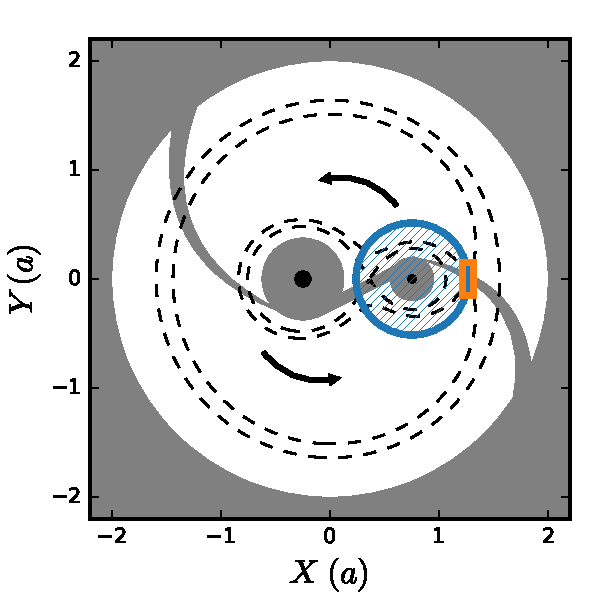
\includegraphics[width=0.8\textwidth]{figures/minidisk/domain.pdf}
\end{center}
\caption{\figlabel{domain} Global sketch of circumbinary accretion.  Shown is a binary black hole system (black dots) with orbital separation $a$ surrounded by a circumbinary gaseous disk (gray solid).  A cavity of radius $2a$ is cleared, and streams from the cavity wall feed ``minidisks'' around each black hole. The L1 and L2 Roche curves are plotted as dotted black lines.  The gas streams enter the vicinity of each black hole through the L2 and L3 Lagrange points.  A gaseous ``bridge'' is seen to exchange gas between minidisks in global Newtonian simulations; for simplicity we do not consider it in this work.  The circular computational domain (thick blue circle) is centered around the secondary black hole and extends to the $L2$ Lagrange point.  Arrows denote the rotation direction of the system; the computational domain co-rotates with the binary.  At the boundary near the incoming stream (thick orange rectangle) a nozzle boundary condition with constant mass injection rate $\dot{M}_\text{nozzle}$ is enforced.  Elsewhere the boundary is a diode.} 
\end{figure}

To model the growth and structure of minidisks, we must specify both the parameters of the binary black hole system and the accretion stream.  The overall mass scale of the binary $M_\text{bin} = M_P+M_S$ sets the overall length scale for the system.  Since we focus on a minidisk around the secondary black hole, we express all lengths in terms of $M = M_S$.  Since we work in units where $c=1$, this also sets the fundamental time scale of the system. The use of physical constants in the cooling prescription \eqrefp{BBcooling} introduces a mass scale $\bar{m}=$ into the system, which scales with $M$ as $\bar{m} \propto M^{5/2}$.  

Our implementation of frame and tidal forces (see \sect{frameforces}) restricts our analysis to large binary separations $a$ and small mass ratios $q$.  We fix $q=0.11$ and $a = 100 M_\text{bin} \approx 1000 M$ for all runs, which satisfies these requirements.  At this separation the corrections to our tidal force prescription are at most $\OO({M_P / a}) \sim 1\%$, but the orbital time scale is still in an accessible regime.  The orbital angular velocity is $\Om_\text{bin} = \sqrt{M_\text{bin} / a^3} \approx 10^{-4} M^{-1}$ and the orbital period is $T_\text{bin} = 2\pi / \Om_\text{bin} \approx 2 \pi \times 10^4 M$.

A circular binary emits GWs that carry away energy and angular momentum and eventually lead to merger.  The time for a circular binary to merge \citep{Peters64}, in units of the initial orbital period, is
\begin{equation}
	T_\text{merge} / T_\text{bin} = \frac{5}{512 \pi}\frac{(1+q)^2}{q} \left(\frac{a}{M_\text{bin}}\right)^{5/2} \ . \eqlabel{Tmerge}
\end{equation}
For the system we consider $a=100 M_\text{bin}$ and $q=0.1$, so $T_\text{merger} \approx 3.7\times 10^3 T_\text{bin}$.  The simulations run for $\approx 30 T_\text{bin}$, so we do not include evolution of the binary orbital parameters at this time.

We model the accretion streams as radial infall through the L2 Lagrange point of the binary, based on global Newtonian simulations of circumbinary accretion \citep{Farris14, Farris15A, Farris15B, DOrazio12, DOrazio16}.  The radial velocity is set to be $v^r = -1/2 v_\text{bin}$, where $v_\text{bin} = \sqrt{M_\text{bin}/a} \approx 0.1$ is the binary orbital velocity.  The angular velocity of the stream is zero in the co-rotating frame.  Since the streams are ballistic, the sound speed should be significantly less than the stream velocity.  To ensure this, we set the pressure in the stream as $\Pi = 5 \times 10^{-6} \Sig$.  Several values of this parameter were used during testing; we found that they did not affect the resulting minidisk. Rather, shock heating and radiative cooling allow the gas to find its own equilibrium temperature once it is incorporated into the disk.  The stream is given a width of $ \De \phi = 0.4$ rad, approximately that of the streams seen in global Newtonian simulations \cite{Farris14}.

The density in the nozzle is set by the accretion rate $\dot{M}$, the main parameter of interest in this study.  The inclusion of dimensionfull $\ka$ and $\sig_{SB}$ parameters in the cooling term breaks the scale invariance of mass energy that would otherwise be present.  Streams of different $\dot{M}$ will cool at different rates relative to the orbital period $T_{\text{bin}}$, leading to hotter or cooler disks.  The density in the stream has a profile $\Sig \propto \cos^2(\pi \phi / \De \phi)$, with the normalization set to match the total accretion rate of specified $\dot{M}$.

The numerical grid is centered on the secondary black hole and extends from $r_\text{in} = 4 M$ to $R_\text{L2} \approx 358 M$, the radius of the L2 Lagrange point. Radial zones are distributed logarithmically, and azimuthal zones are placed to keep the aspect ratio of cells close to unity. The stream extends over $\phi \in [-\De \phi / 2, \De \phi / 2] rad$, boundary cells within the stream are fixed to their local stream values. On the outer boundary away from the stream a diode boundary condition is used: zero gradient in all fluid variables with the radial velocity restricted to be positive or zero.

At the inner boundary a hybrid boundary condition is used.  The fluid velocity is set to be exactly as given in \eq{Ugeo}, appropriate for ballistic matter infalling on geodesics.  The density is set to be $\Sig = -\dot{M} / r U^r \De \phi_\text{cell}$, where $\dot{M}$ is calculated from the innermost non-boundary annulus and $\De \phi_\text{cell}$ is the angular width of the cell.  Given $\Sig$, the pressure $\Pi$ is set to ensure isentropic infall.

Although the inner boundary is outside the event horizon, we find that it does not affect the evolution of the system.  This is because it is still inside the sonic radius of the flow, so no information can propagate out to the minidisk itself.  See the discussion in \sect{bc} and \fig{bc_hr_comp} for details. The CFL limited time step $\De t$ is controlled by the innermost zones of the grid, where the radial velocity is large (due to the black hole) and the cells are narrow.  Placing the inner boundary above the event horizon allows for much larger time steps than otherwise possible; keeping it below the sonic point ensures the fidelity of the simulation.  We found $r_{in} = 4M$ to be a good choice.

The initial condition for each minidisk is an $\al=10^{-3}$ Novikov--Thorne accretion disk with $\dot{M}$ set equal to the nozzle rate \citep{Novikov73}.  

\begin{table}
\begin{center}
\begin{tabular}{ccccccc}
\hline \hline
Name &${\dot{M}}^a$ & $r_\text{in}$ & $q$ & $N_r$ & ${T_\text{start}}^b$ & ${T_\text{end}}^b$ \\ [0.5ex]
\hline
\model{1} & $1.9\times10^{3}$  & $4M$ & $0.11$ & $256$ & $0$ & $29$ \\
\model{1.5} & $5.8\times10^{2}$ & $4M$ & $0.11$ & $256$ & $0$ & $29$ \\
\model{2} & $1.9\times10^{2}$ &  $4M$ & $0.11$ & $256$ & $0$ & $29$ \\
\model{2.5} & $5.8\times10^{1}$ & $4M$ & $0.11$ & $256$ & $0$ & $25$ \\
\model{3} & $1.9\times10^{1}$ & $4M$ & $0.11$ & $256$ & $0$ & $29$ \\
\model{2-hr} & $1.9\times10^{2}$ & $4M$ & $0.11$ & $512$ & $28$ & $32$ \\
\model{2-bc} & $1.9\times10^{2}$ & $1.8M$ & $0.11$ & $256$ & $25$ & $26$ \\ [0.5ex]
\hline
\multicolumn{7}{l}{\textsuperscript{a}$\dot{M}$ is given in code units and scales as $M^{3/2}$.}\\
\multicolumn{7}{l}{\textsuperscript{b}$T_\text{start}$ and $T_\text{end}$ are given in units of $T_\text{bin}$.}
\end{tabular}
\end{center}
\caption{Minidisk Models \label{tb:models}}
\end{table}


The five primary minidisk models in this study are summarized in \tab{models}.  The accretion rate is given in code units, which scale as $M^{3/2}$.  If $M=M_{\odot}$, the accretion rate for \model{2} corresponds to $2\times10^{-3} M_{\odot} \text{yr}^{-1}$.  At this scale $T_\text{bin} = 0.3$ s and $T_\text{merge} = 20$ minutes.  For an SMBHB with $M_\text{bin} = 10^6 M_{\odot}$, $T_\text{bin} = 8.6$ hr and $T_\text{merge} = 3.7$ yr.  Two tests, Models \texttt{2-hr} and \texttt{2-bc}, were run to check dependence on numerical resolution and the inner boundary condition, respectively. Due to resource constraints, \model{2-bc} was only run for a single orbit, and \model{2-hr} for four orbits.

\subsection{Fiducial Run}
\sectlabel{fiducial}

We take the $\dot{M} = 2 \times 10^{-3} M_\odot \text{yr}^{-1}$ model (\model{2}) as our fiducial run.  The accretion rate through the inner ($r=4 M$) and outer ($r=r_\text{L2}$) boundaries is plotted as a function of time in \fig{mdot-fid}. The initial disk has a surface density much higher than the stream from L2 (\fig{sig-fid-0}).  In the first orbit the initial disk develops its own tightly wound two-armed spiral as the gas in the outer radii is flung away.  The two-armed spiral begins tightly wound and diffuse, but quickly sharpens into a shock and begins to open as the disk heats (\fig{sig-fid-05}).  Some gas flung to the boundary falls back, and accretion proceeds in clumps for the first two orbits (\fig{sig-fid-2}).  After two orbits, the bulk of the initial disk has either been accreted or thrown out the outer boundary.  As the remaining disk accretes, it becomes more diffuse and cools, the spiral shocks tighten, and the accretion rate drops (\fig{sig-fid-5}).

\begin{figure}
\begin{center}
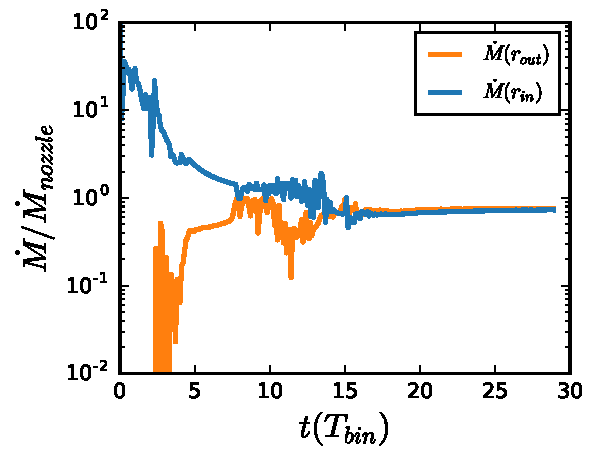
\includegraphics[width=0.8\textwidth]{figures/minidisk/q011_m3_mdot.pdf}
\end{center}
\caption{\figlabel{mdot-fid} Time series of the accretion rate (measured as a fraction of the nozzle mass injection rate) through the inner (blue) and outer (orange) boundaries of \model{2}.  After $\sim17$ orbits the inner and outer accretion rates balance, indicating the onset of a quasi-steady state.}
\end{figure}

\begin{figure}
\begin{center}
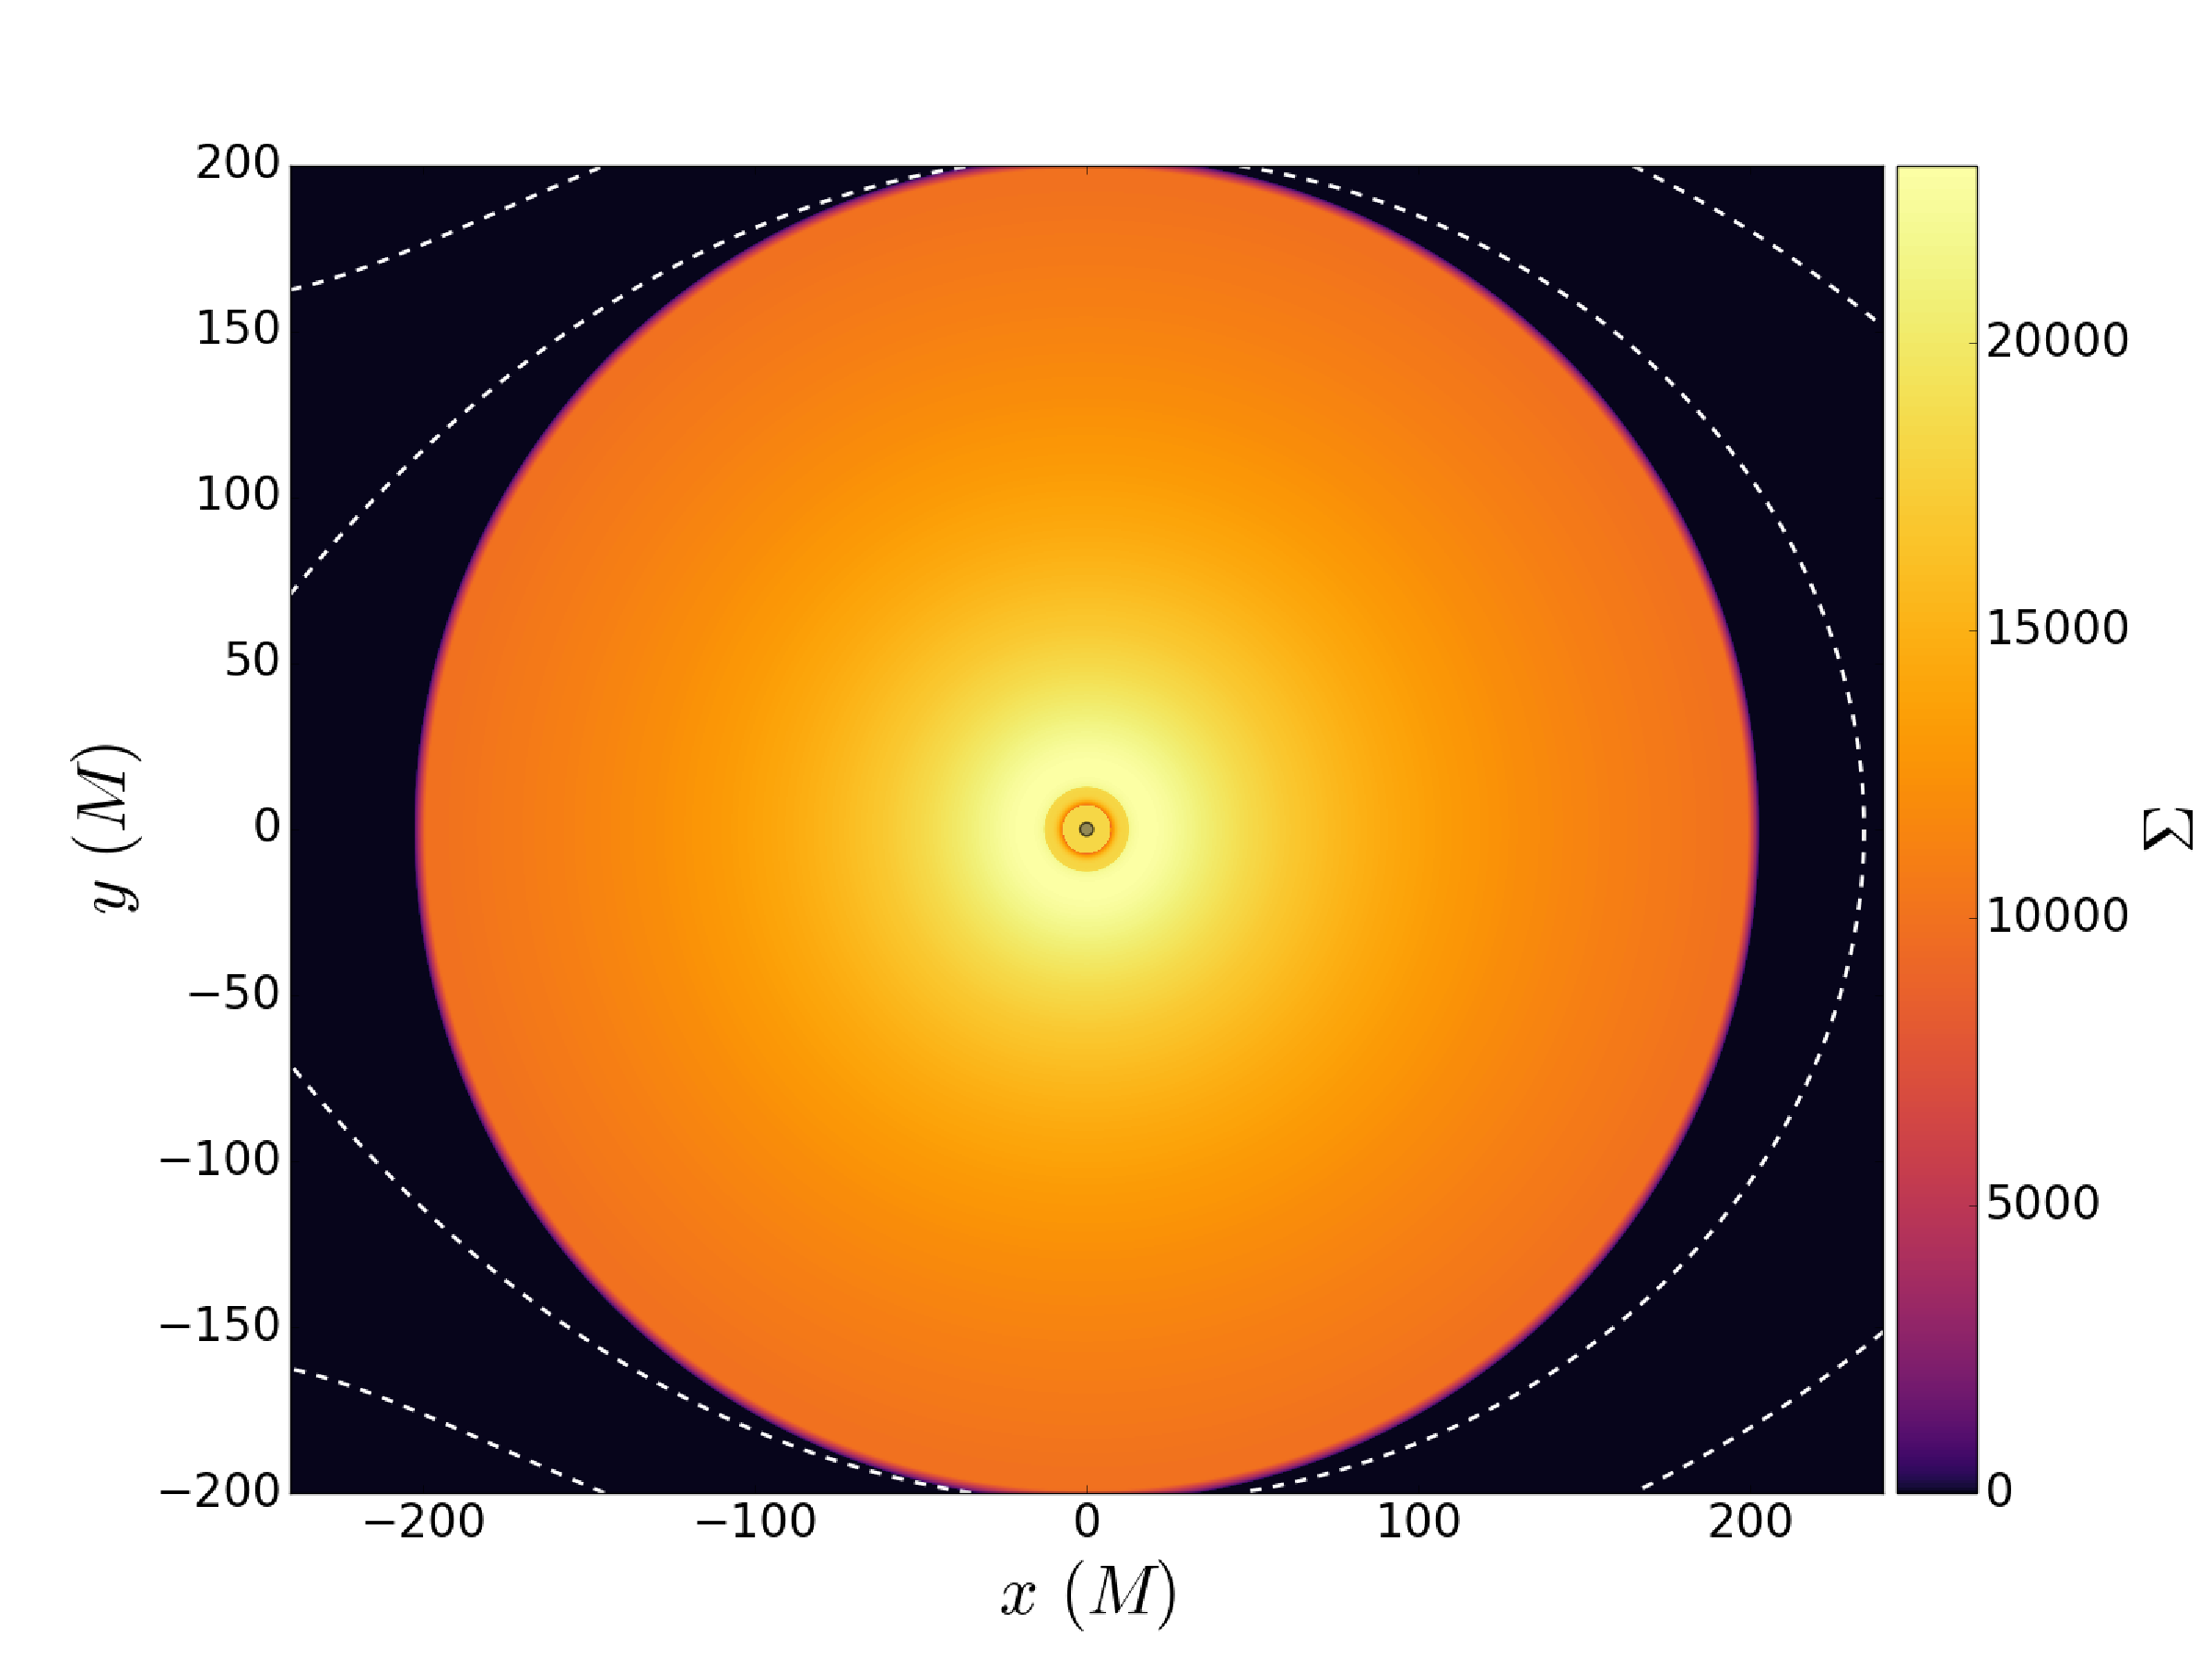
\includegraphics[width=0.8\textwidth]{figures/minidisk/q011_m3_sig_0000.pdf}
\end{center}
\caption{\figlabel{sig-fid-0} Initial surface density for fiducial minidisk.  Magenta dashed lines are level curves of the Roche potential corresponding to the L1 and L2 Lagrange points.}
\end{figure}

\begin{figure}
\begin{center}
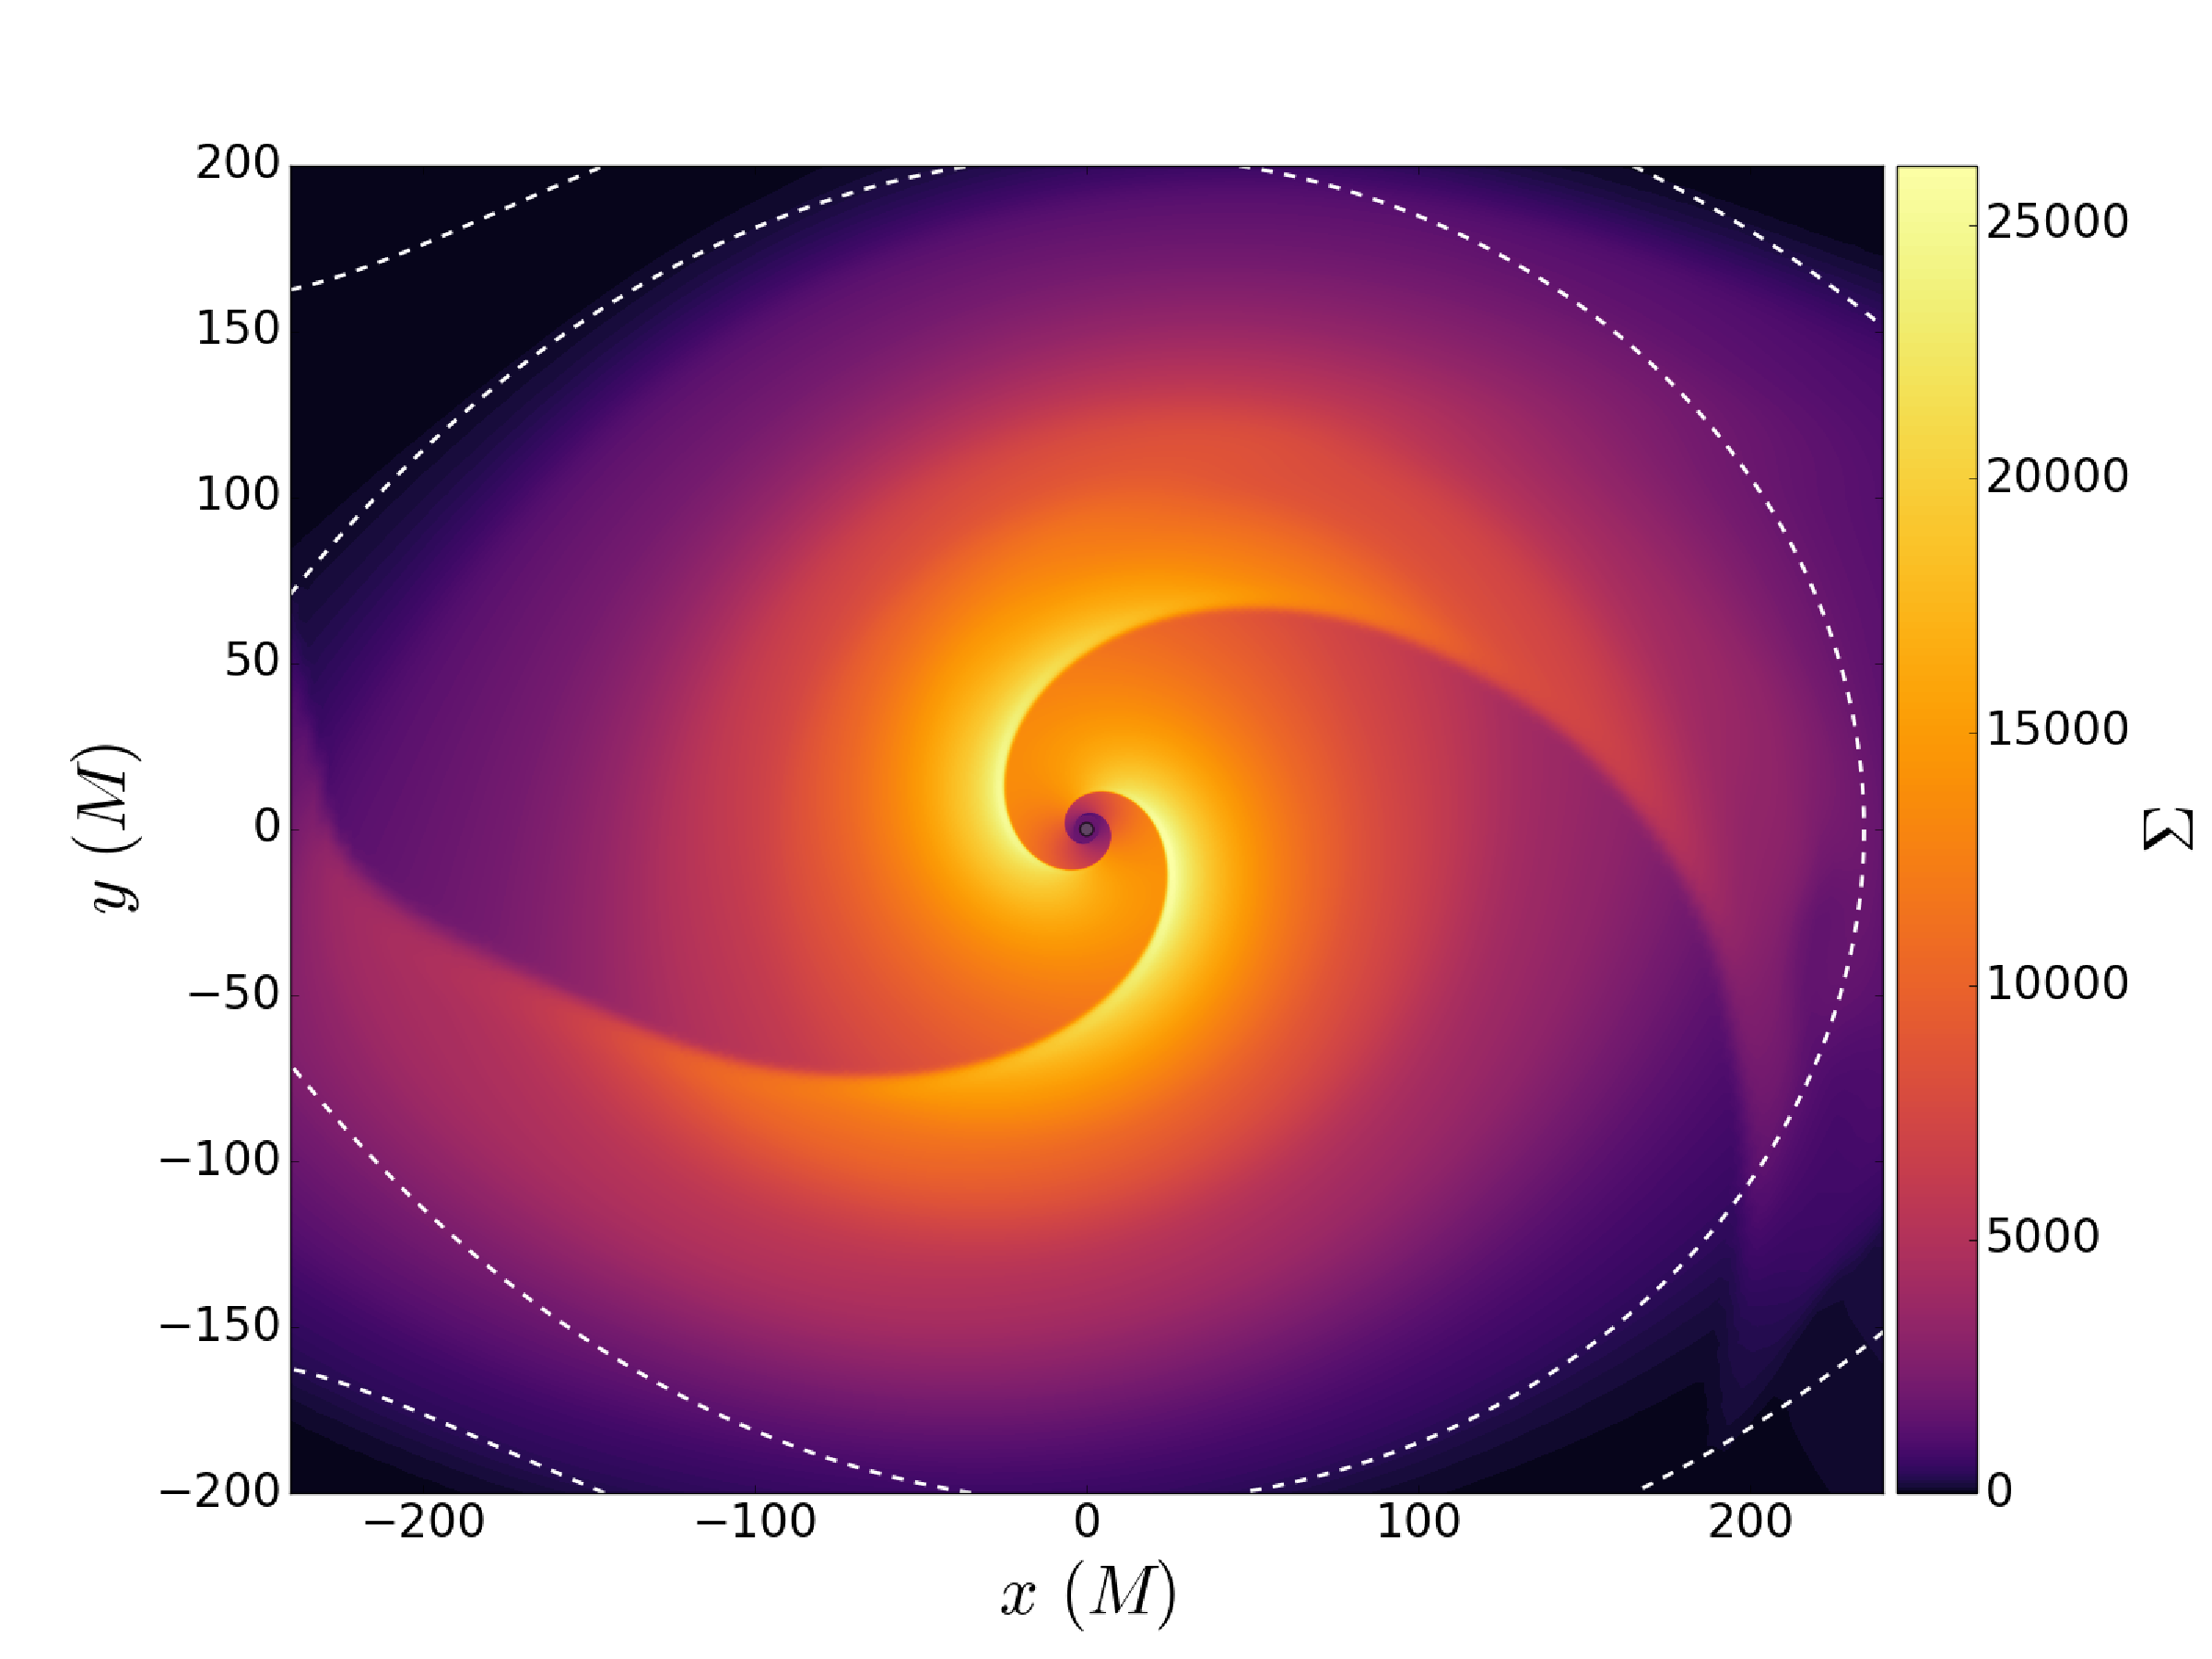
\includegraphics[width=0.8\textwidth]{figures/minidisk/q011_m3_sig_0050.pdf}
\end{center}
\caption{\figlabel{sig-fid-05} Same as \fig{sig-fid-0}, but at $t = 1/2\ T_\text{bin}$.  The initial disk quickly develops spiral shocks.}
\end{figure}

\begin{figure}
\begin{center}
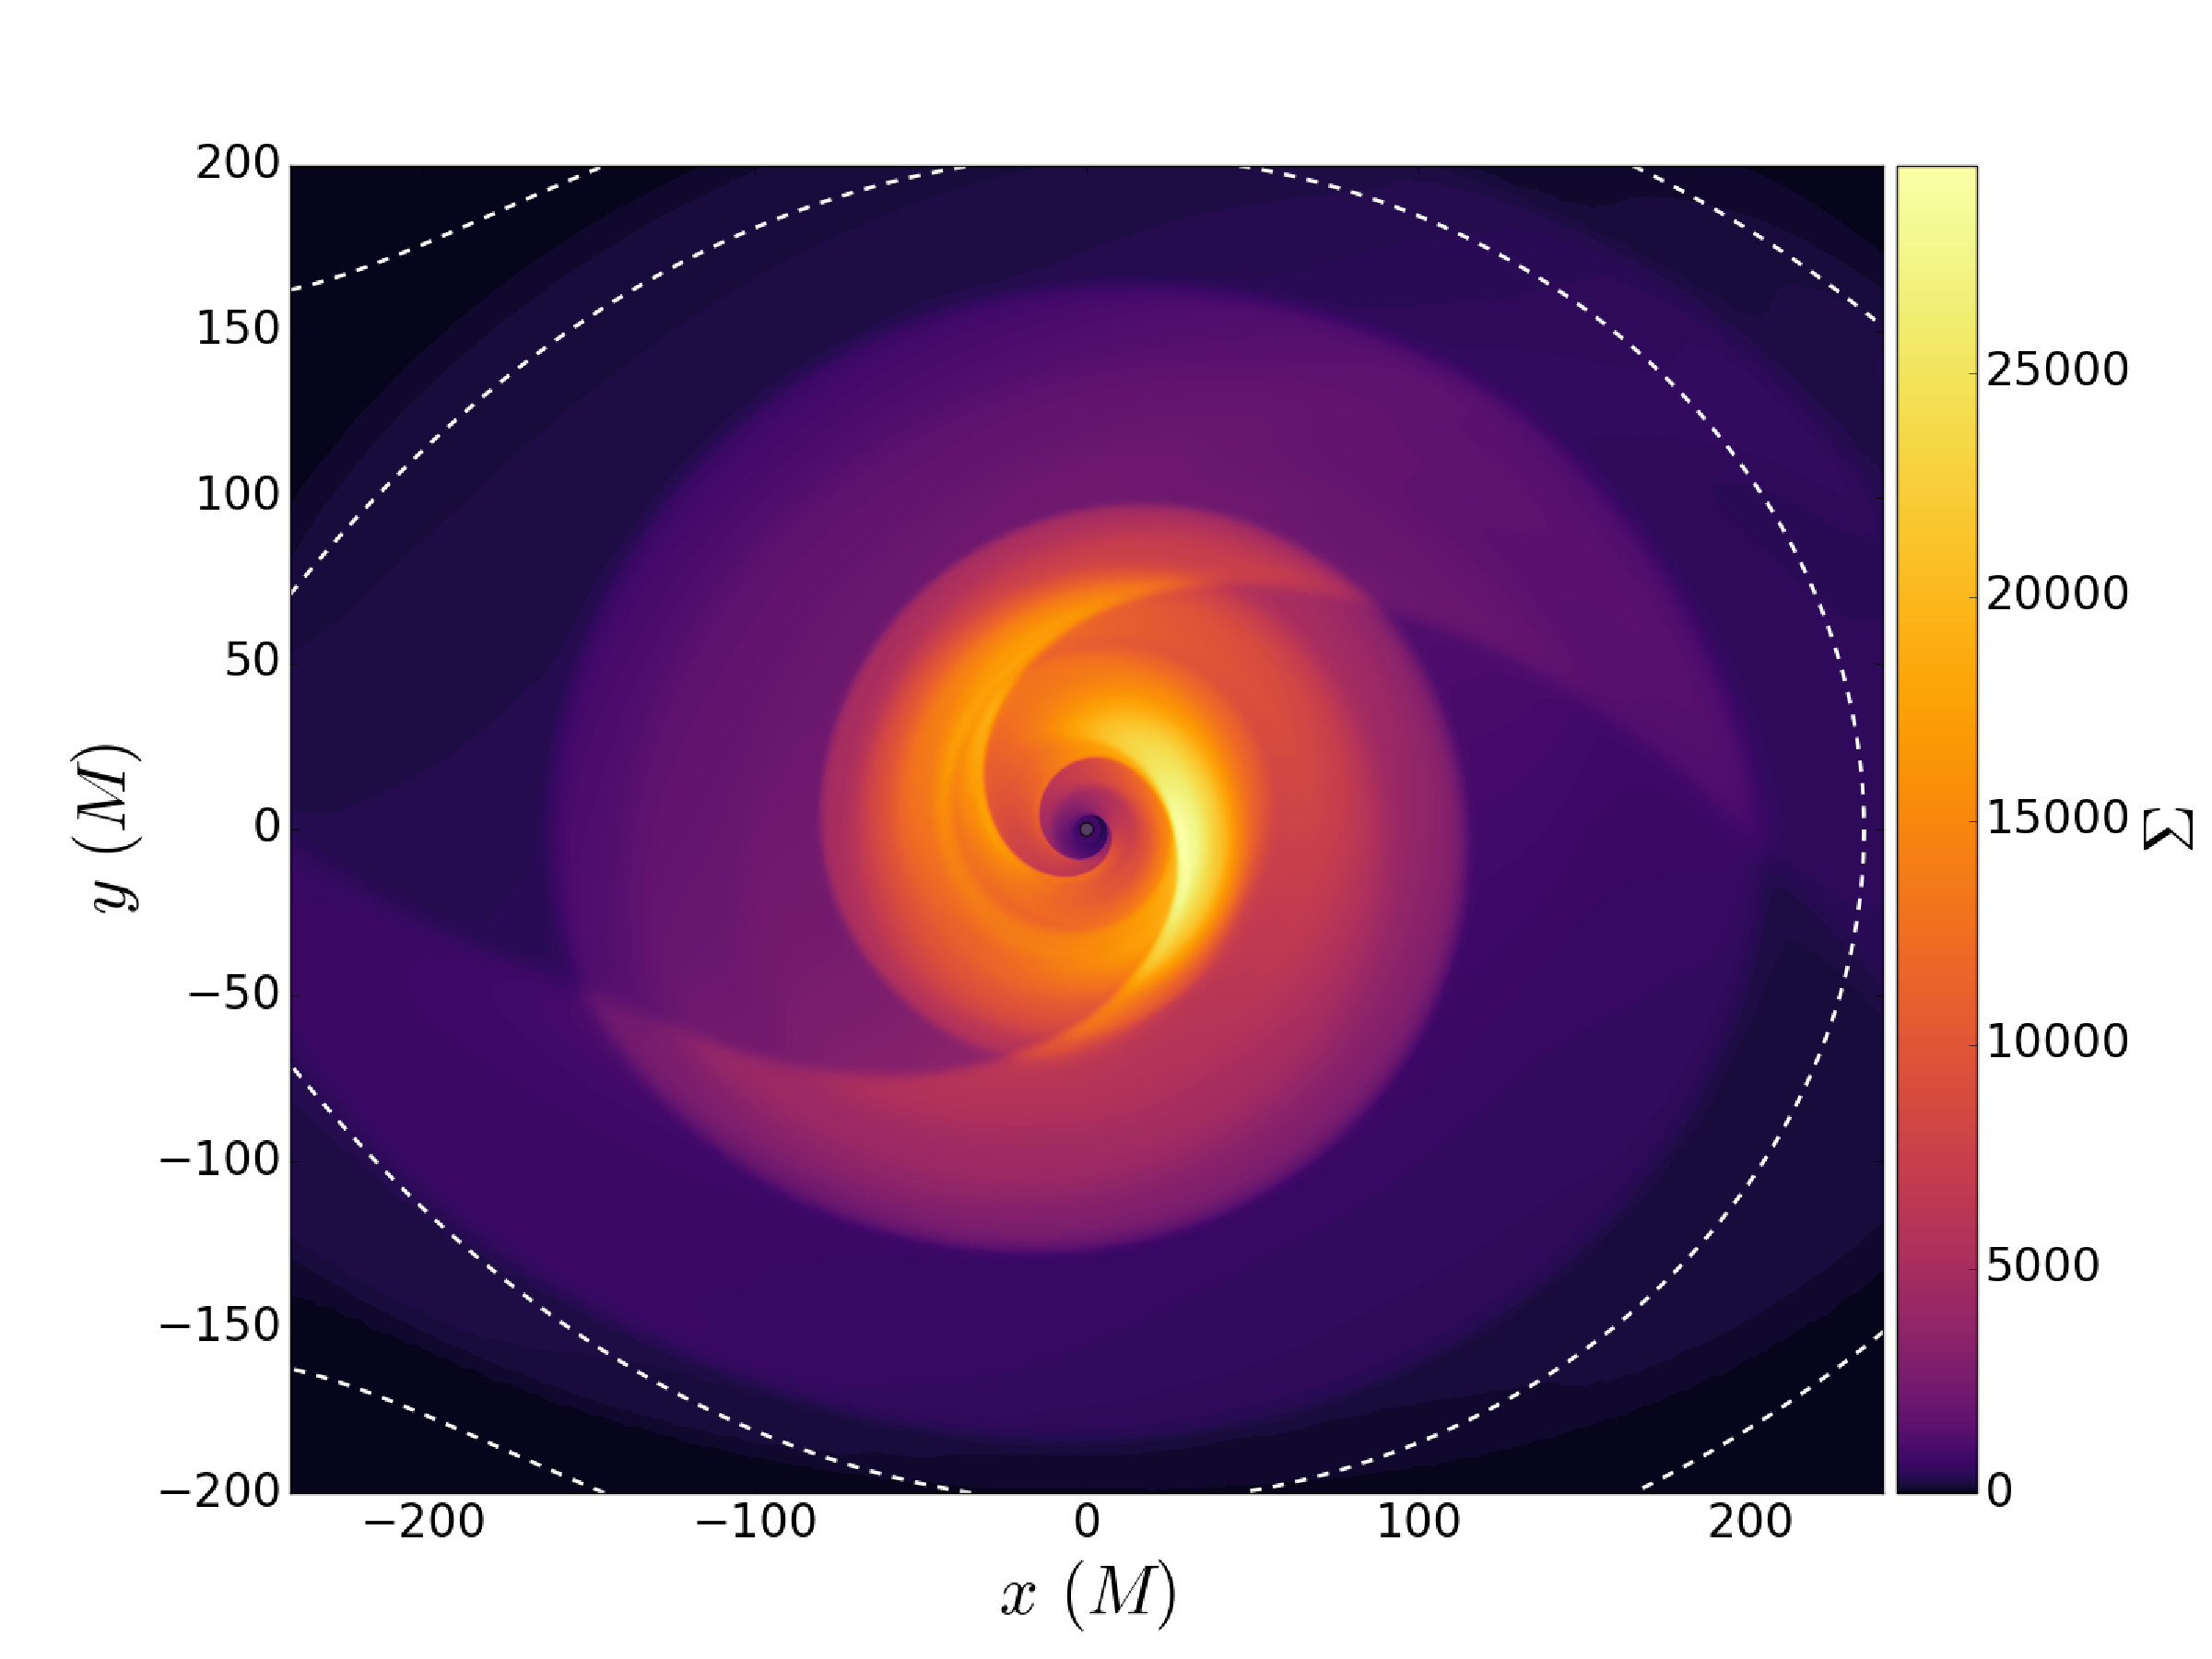
\includegraphics[width=0.8\textwidth]{figures/minidisk/q011_m3_sig_0200.pdf}
\end{center}
\caption{\figlabel{sig-fid-2} Same as \fig{sig-fid-0}, but at $t = 2 T_\text{bin}$.  Accretion proceeds in clumps as gas from the initial disk is either thrown out of the domain or falls into the black hole.}
\end{figure}

\begin{figure}
\begin{center}
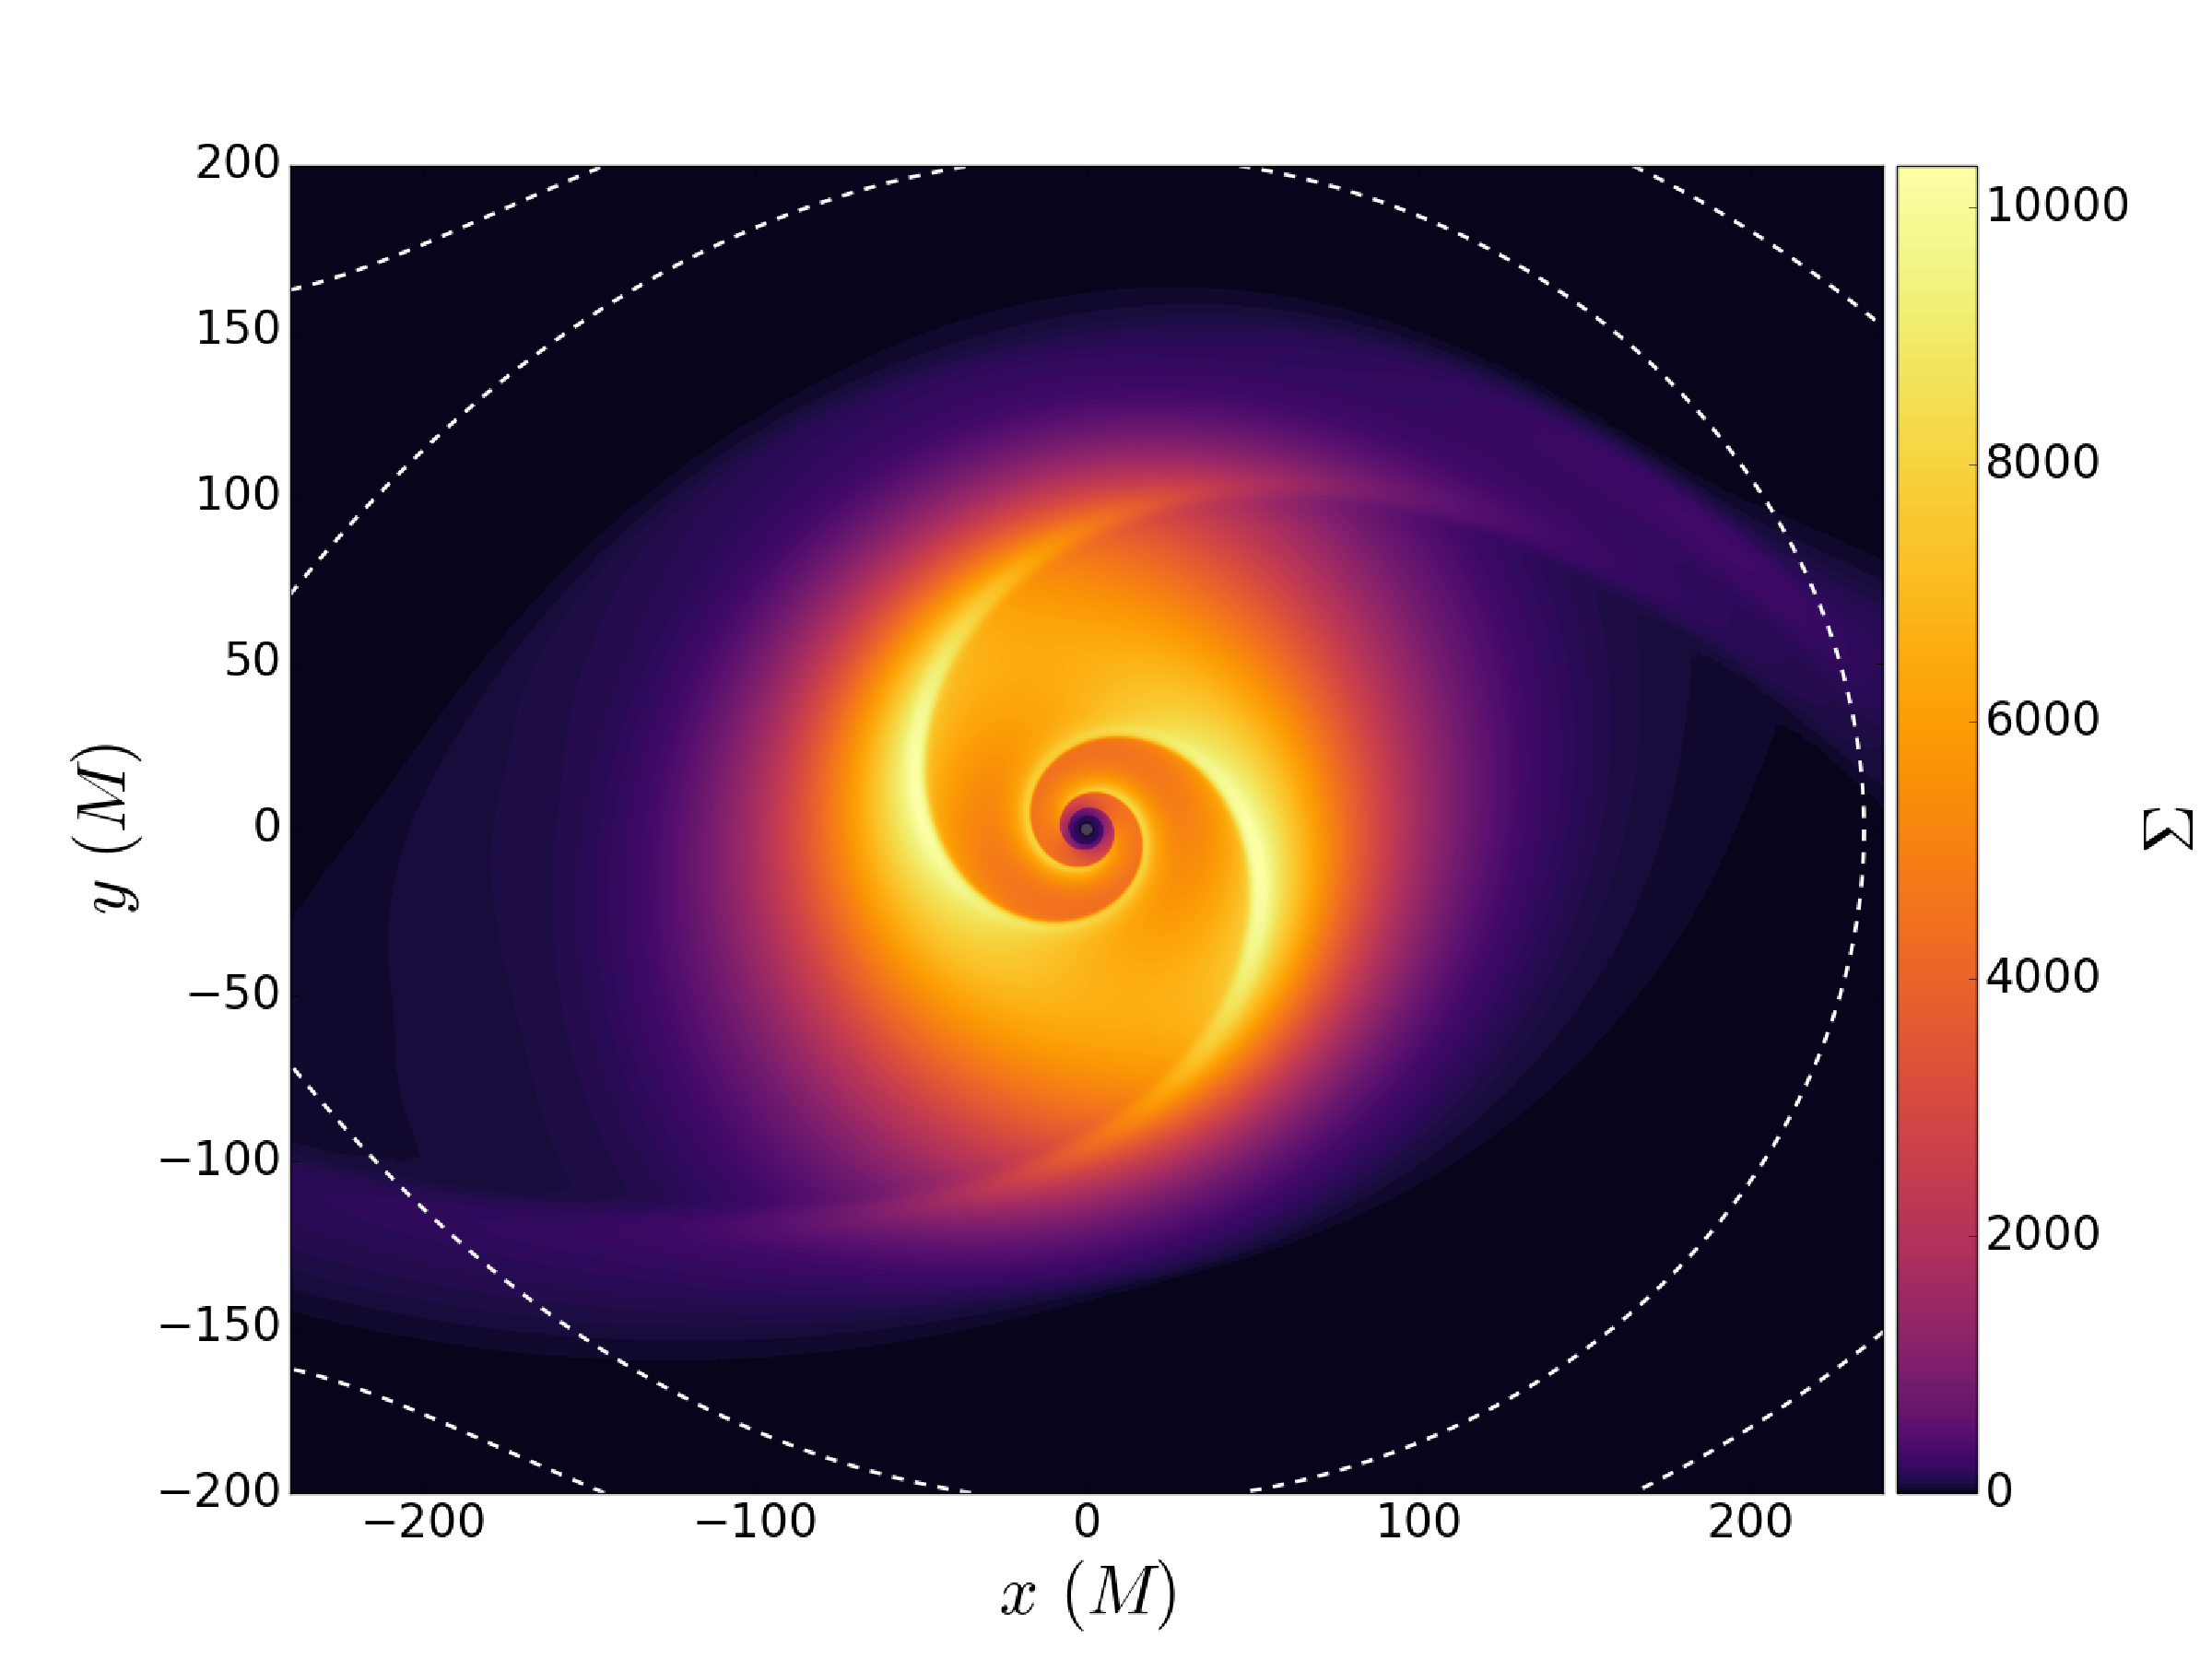
\includegraphics[width=0.8\textwidth]{figures/minidisk/q011_m3_sig_0500.pdf}
\end{center}
\caption{\figlabel{sig-fid-5} Same as \fig{sig-fid-0}, but at $t = 5 T_\text{bin}$.  Most of the initial gas has left. The accretion rate drops as the disk cools.}
\end{figure}

\begin{figure}
\begin{center}
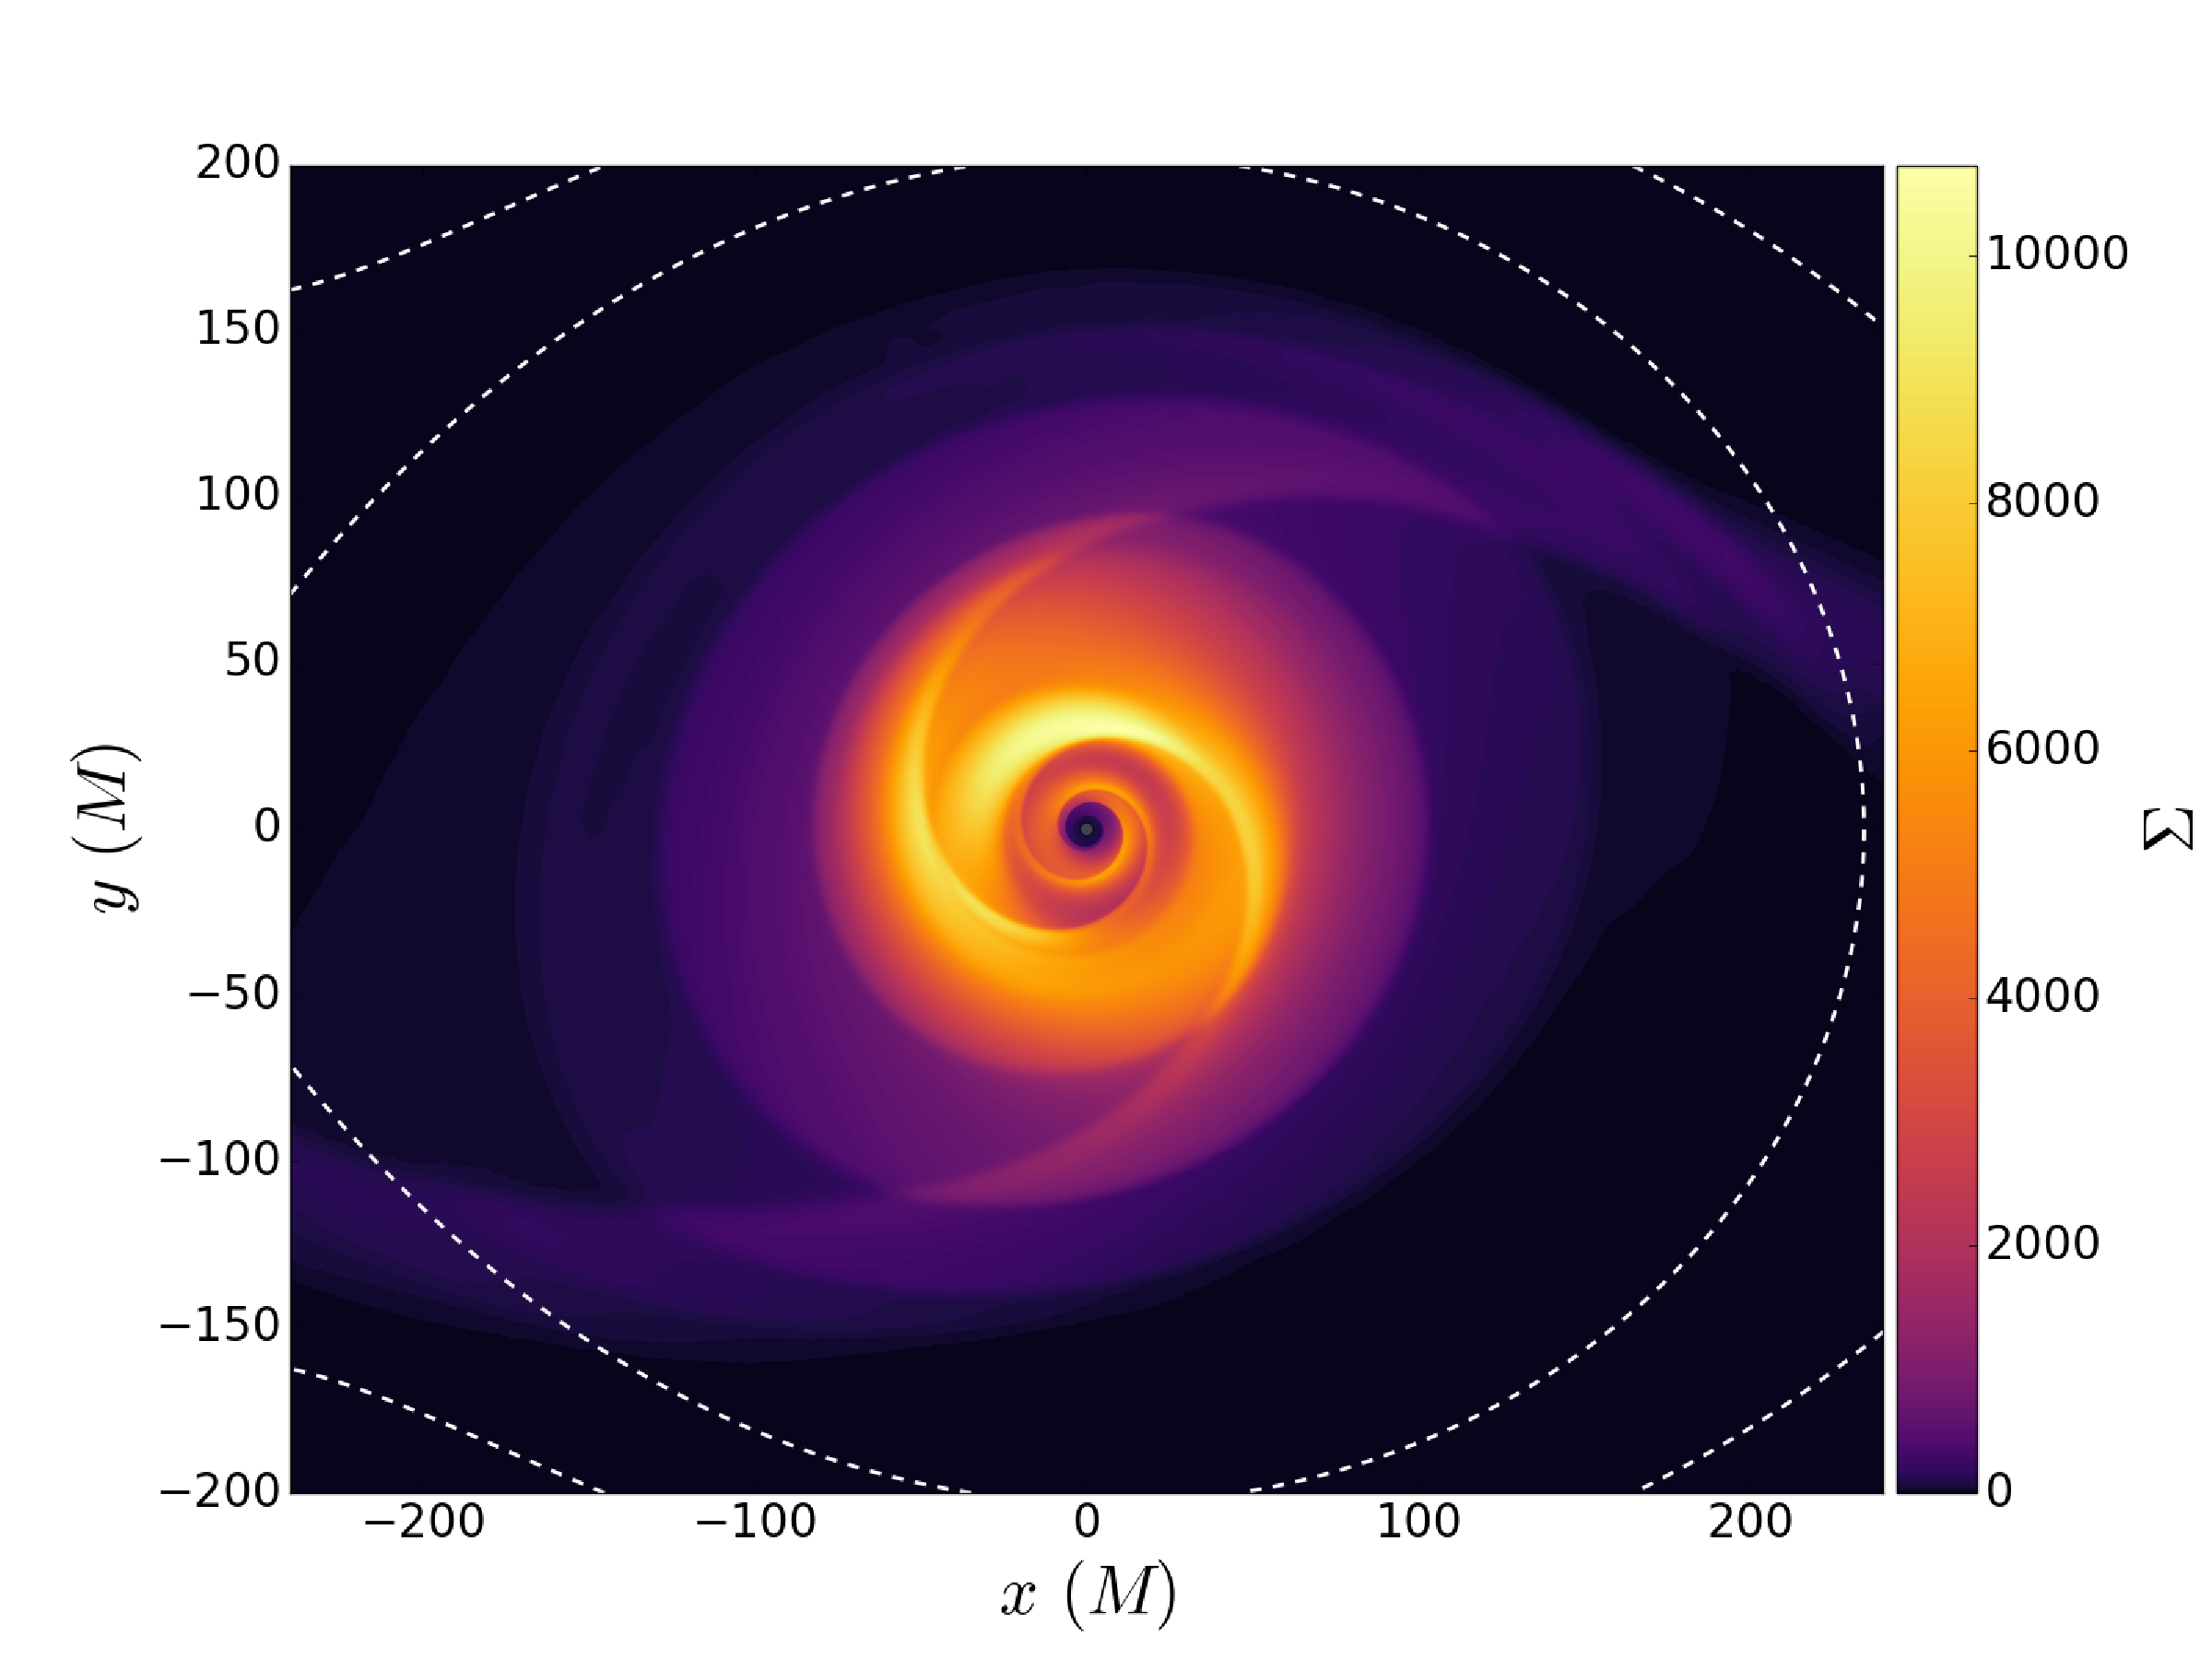
\includegraphics[width=0.8\textwidth]{figures/minidisk/q011_m3_sig_1300.pdf}
\end{center}
\caption{\figlabel{sig-fid-13} Same as \fig{sig-fid-0}, but at $t = 13 T_\text{bin}$.  Variability sets in as the disk begins interacting dynamically with the accretion stream.}
\end{figure}


At $t\sim 8 T_\text{bin}$ the accretion rate through the disk becomes comparable to the stream.  For the next eight orbits a complicated and turbulent interaction occurs between the disk and stream.  The stream begins wobbling and sending gas to the disk in clumps.  Clumps execute an orbit of the black hole and collide with the original stream, causing it to wobble further, producing more clumps.  The clumps are sheared by the accretion flow, and after many orbits within the disk, they are accreted. The spiral shocks retain their structure through the clumpy accretion (\fig{sig-fid-13}).

At $t\sim17 T_\text{bin}$ the disk--stream interaction stabilizes and the disk reaches a quasi-steady state.  The accretion rate through the inner boundary matches the inflow rate through the outer boundary, and the two-armed spiral shocks lock into a constant pattern.  Small-scale flows still occur as gas slowly redistributes within the disk, relaxing to a true steady state.  The simulation ends at $T\sim30 T_\text{bin}$ (\fig{sig-fid-28}), before this secular evolution ends.

\begin{figure*}
\begin{center}
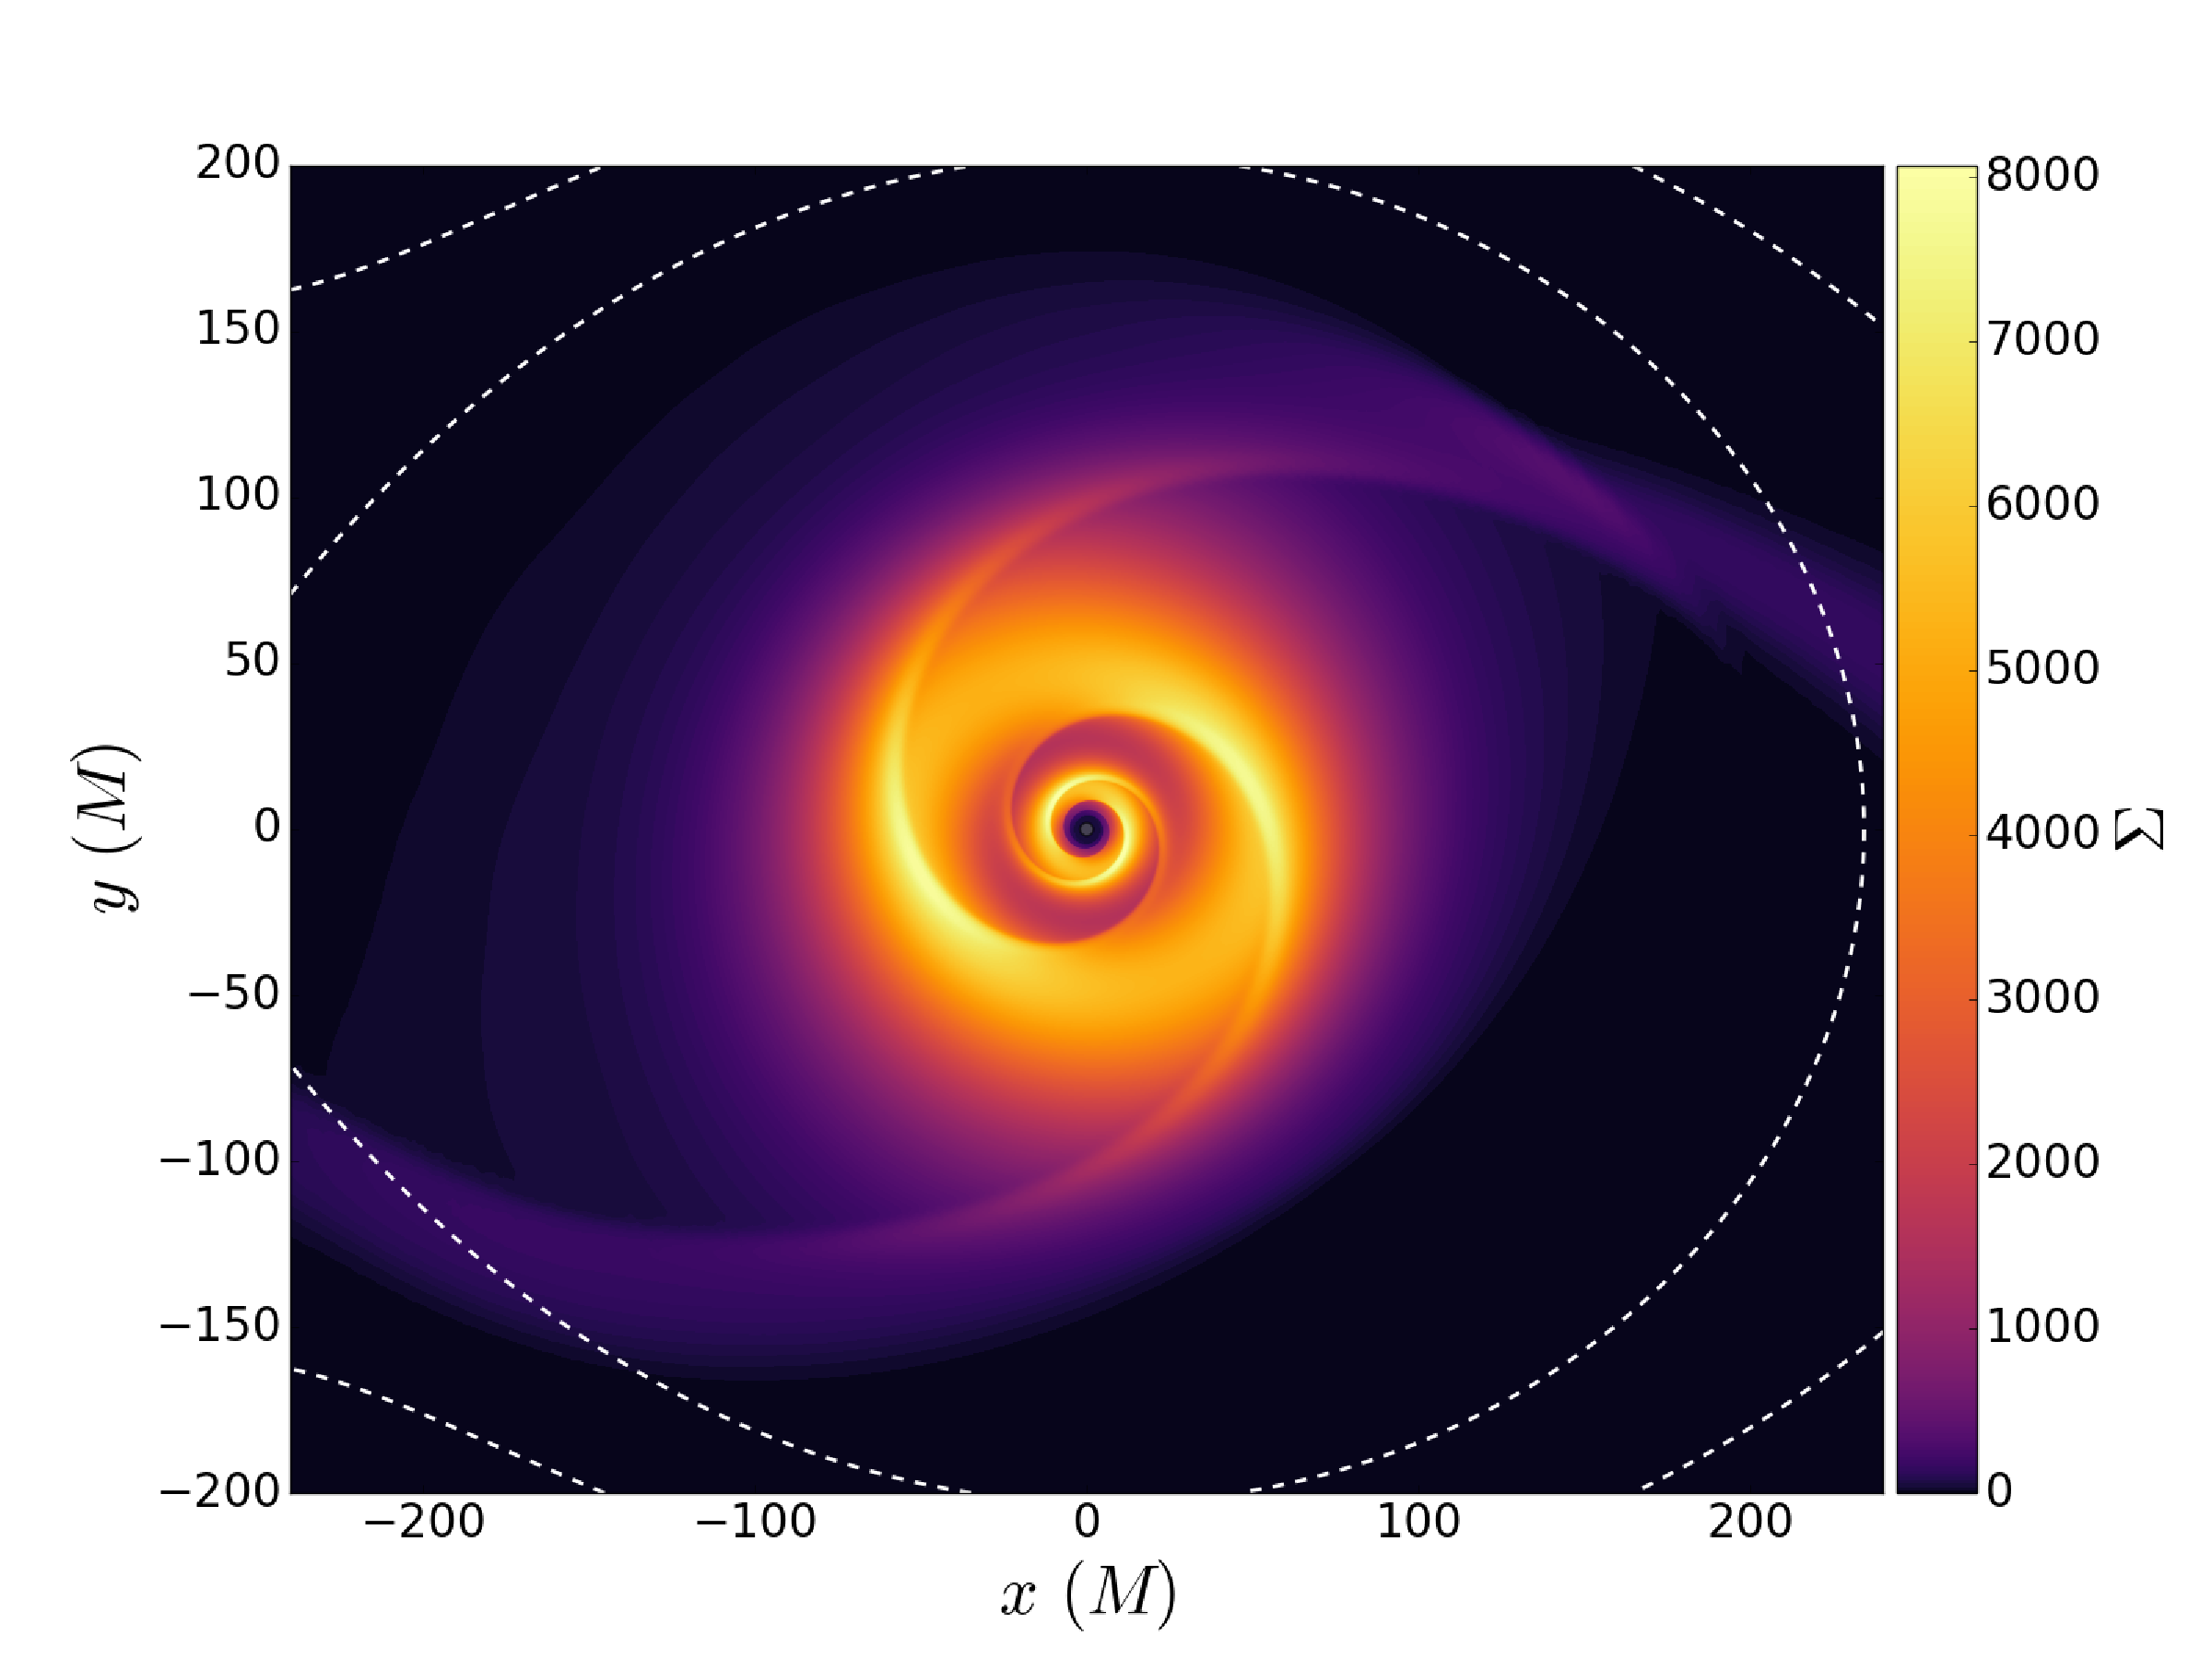
\includegraphics[width=0.8\textwidth]{figures/minidisk/q011_m3_sig_2800.pdf}
\end{center}
\caption{\figlabel{sig-fid-28} Same as \fig{sig-fid-0}, but at $t = 28 T_\text{bin}$.  The disk in a quasi-steady state.}
\end{figure*}


%%%%%
%Section 4 - Analysis
%%%%%

\section{Analysis}
\sectlabel{analysis}


%%% Shock Detection %%%
\subsection{Shock Detection}
\sectlabel{shockDet}

To characterize the role of spiral shocks, we first must find them in the simulation output.  We use a modified version of the relativistic shock detector presented in \cite{Zanotti10}.  The basic algorithm classifies adjacent zones (e.g. in the $\phi$ direction) by considering the Riemann problem at their interface.  Interfaces are classified as shocks if the Riemann problem solution requires at least one shock.  We find this to be too sensitive a criterion, so we add additional constraints for an interface to be considered a shock.

In the simple algorithm, first the relative normal velocity $v_{12}$ is calculated.  Assuming $\phi$-separated cells $1$ and $2$ with $\Pi_1 > \Pi_2$, this is
\begin{equation}
	v_{12} = \frac{v^{\hat{\phi}}_1 - v^{\hat{\phi}}_2}{1 - v^{\hat{\phi}}_1 v^{\hat{\phi}}_2} \ . \eqlabel{vrel}
\end{equation}
In the above $v^{\hat{\phi}}$ is the azimuthal 3-velocity in an orthonormal frame. The relative velocity $v_{12}$ is compared to the critical velocity $(\tilde{v}_{12})_{\mathcal{R} \mathcal{S}}$:
\begin{equation}
	(v_{12})_{\mathcal{R}\mathcal{S}} = \tanh \int_{\Pi_1}^{\Pi_2} \frac{\sqrt{h(\Pi)^2 + \mathcal{A}_1^2(1-c_s(\Pi)^2)}}{(h(\Pi)^2 + \mathcal{A}_1^2)\Sig(\Pi) c_s(\Pi)} \dd \Pi \ . \eqlabel{vrs}
\end{equation}  
In the integral in \eq{vrs}, thermodynamic quantities $h$, $c_s$, and $\Sig$ are calculated at the specific entropy $s_1$ of cell 1 and $\mathcal{A}_1 = h_1 u_1^{\hat{r}}$.  This velocity is the largest normal velocity that a single rarefaction wave can provide between cells 1 and 2    \citep{Rezzolla03}.  If $v_{12} > (\tilde{v}_{12})_{\mathcal{R}\mathcal{S}}$ a shock is necessarily present.

We find the criterion $v_{12} > (\tilde{v}_{12})_{\mathcal{R}\mathcal{S}}$ alone to be far too sensitive, so to consider an interface a shock, we require $v_{12} - (\tilde{v}_{12})_{\mathcal{R}\mathcal{S}} > \Delta v_{amb}$, where $\Delta v_{amb}$ is a threshold value.  Lastly, we require the specific entropy to increase in the direction of the flow: $u^\phi \partial_\phi s > 0$.

Our full shock detector algorithm runs on each annulus of the computational grid.  Since the shocks tend to have small pitch angles, they have small radial width but may extend over a few zones azimuthally.  The algorithm identifies all zones in the annulus separated by a shock via our criteria above and groups them into contiguous segments.  The two segments with the largest values of $v_{12} -  (\tilde{v}_{12})_{\mathcal{R}\mathcal{S}} $ are classified as the shocks. The threshold $\Delta v_{amb}$ is set for each annulus to be the larger of $0$ or the fourth-largest maxima of $v_{12} -  (\tilde{v}_{12})_{\mathcal{R}\mathcal{S}} $. We find this value to have good discriminatory power for these runs, picking out the shocks but ignoring the ambient flow.

The final output of the shock detector is the position $\Phi(r)$ for the leading and trailing edge of both shock waves at each annulus of the computational grid.

\subsection{Wave Propagation}

A linear perturbation to a fluid quantity of azimuthal mode $m$ and pattern speed $\Omega_P$ can be written as
\begin{equation}
	\delta X(t, r, \phi) = \tilde{X}_{m,\omega}(r) \exp \left( i \int_r k(r) \dd r  + i m (\phi - \Omega_P t) \right)\ . \eqlabel{pert}
\end{equation}
Such perturbations are spirals with pitch angle
\begin{equation}
	\tan \theta = m / k r \ . \eqlabel{pitch}
\end{equation}

The hydrodynamics equations for such a mode reduce to a system of ordinary differential equations in the radial coordinate $r$.  In the `tight winding' limit $k \gg \tilde{X}'/\tilde{X}$, the perturbation is highly oscillatory, and the WKB approximation may be used to yield the well-known \citep{Binney08} dispersion relation for tightly wound waves in a Newtonian gaseous disk:

\begin{equation}
	\Omega^2 - m^2(\Omega-\Omega_P)^2 + c_s^2 k^2 = 0 \ . \eqlabel{dispNewt}
\end{equation}
The generalization of \eq{dispNewt} to a disk in the Schwarzschild metric is straightforward \citep{Perez97}.  The background state is a steady thin disk of sound speed $c_s \ll 1$ and velocity given by \eq{Ugeo} in the region $r > r_{ISCO}$.  Assuming that the perturbation is adiabatic, tightly wound, and neglecting vertical structure leads to the dispersion relation for relativistic $p$-modes \citep{Abramowicz13}:
\begin{equation}
	\left(1-\frac{6M}{r} \right)\left(U^\phi\right)^2 - m^2(U^\phi-U^0\Omega_P)^2 + g_{rr} c_s^2 k^2 = 0 \ . \eqlabel{disprel}
\end{equation}
In Schwarzschild coordinates the perturbation remains a spiral with pitch angle \eqrefp{pitch}.  The dispersion relation can be solved for the radial wavenumber $k$ yielding
\begin{align}
	\tan \theta &= \left( \frac{r U^\phi}{c_s} \right)^{-1} \left(1-\frac{2M}{r}\right)^{\frac{1}{2}} \eqlabel{dispRelPitch} \\ \nonumber
		&\times \left(\left(1- \frac{U^0 \Omega_P}{U^\phi}\right)^2 - \frac{1}{m^2}\left(1-\frac{6M}{r}\right)\right)^{-\frac{1}{2}}\ . 
\end{align}
Shocks, of course, are intrinsically nonlinear perturbations to a fluid flow.  Weak shocks, however, travel very near the local sound speed and can be approximated as linear waves.  The degree to which spiral shocks in the minidisks satisfy \eq{dispRelPitch} can be used to gauge their nonlinearity.  

\subsection{Angular Momentum Decomposition}
\sectlabel{angMomDecom}

A detailed look at the angular momentum transport due to spiral shocks requires a decomposition of the various torques acting on the system. Defining angular integrated quantities as $\avet{\cdot} = \int \dd \phi \sqrt{-g} (\cdot)$, we can write effective 1D continuity and angular momentum equations \eqrefp{GRHD} in a coordinate frame:
\begin{align}
	\partial_t \ave{\Sig u^0} + \partial_r \ave{\Sig u^r} &= 0 \ ,\eqlabel{aveAng}\\
	\partial_t \ave{\Sig h u^0 u_\phi} + \partial_r \ave{\Sig h u^r u_\phi} &= \ave{f_\phi}- \ave{u_\phi \dot{Q}_{cool}} \ .\nonumber
\end{align} 
We can decompose \eq{aveAng} by separating the part that strictly obeys the continuity equation.  First, define
\begin{align*}
	\aveRe{\Sig h u^\mu u_\phi} &= \ave{\Sig h u^\mu u_\phi} - \ave{\Sig u^\mu} \ell \ , \\
	\ell &= \frac{\ave{\Sig h u^0 u_\phi}}{\ave{\Sig u^0} } \ .
\end{align*}
We can then write angular momentum conservation as
\begin{equation}
	\ave{\Sig u^\mu} \partial_\mu \ell + \partial_\mu \aveRe{\Sig h u^\mu u_\phi} =  \ave{f_\phi}- \langle u_\phi \dot{Q}_\text{cool} \rangle \ , 
\end{equation}
or
\begin{align}
	\ave{\Sig u^0} \partial_t \ell &= \dot{M} \partial_r \ell -  \partial_r \aveRe{\Sig h u^r u_\phi} +  \ave{f_\phi}- \langle u_\phi \dot{Q}_\text{cool} \rangle \ , \nonumber \\
	&\equiv \tau_{\dot{M}} + \tau_\text{Re} + \tau_\text{ext} + \tau_\text{cool} \ . \eqlabel{angMomDecom}
\end{align} 
\eq{angMomDecom} decomposes the rate of change of angular momentum into four contributions: accretion ($\tau_{\dot{M}}$), Reynolds-type stress ($\tau_\text{Re}$), external torques ($\tau_\text{ext}$), and cooling ($\tau_\text{cool}$).  Accretion torque is due to the bulk flow of gas over a radially varying specific angular momentum profile. The Reynolds torque is due to nonaxisymmetric structures in the flow, particularly varying azimuthal profiles of radial mass flux and specific angular momentum. External torques in our case are completely due to the presence of the binary companion. The cooling torque $\tau_\text{cool}$ is a purely relativistic effect, representing the loss of momentum to photons. It is small so long as the rest-mass energy density is greater than the thermal energy of the gas.

\subsection{Ray-traced Spectra}
\sectlabel{raySpec}

Using the physical cooling prescription \eqrefp{BBcooling} gives us the ability to self-consistently calculate the electromagnetic emission of our minidisk models.  Since the bulk of the emission comes from the innermost regions of the disk, a radiative transfer simulation in the curved spacetime of the black hole is necessary to accurately produce an observational spectrum.

We follow the method of \cite{Kulkarni11} and \cite{Zhu12} to perform the radiative transfer.  We set up an image plane a large distance $d = 10^6 M$ from the central black hole.  The flux through the image plane is
\begin{equation}
	F_\nu = \frac{1}{d^2} \int \dd A I_\nu \ ,
\end{equation}
where $I_\nu$ is the specific intensity at the image plane.  Null rays $k^\mu$ are integrated from the image plane through the Schwarzschild spacetime to the disk surface at $z=0$.  The effects of finite disk height were investigated in \cite{Kulkarni11}, and found to be negligible for moderate observer inclination angles $i$. Assuming vacuum between the image plane and disk, $I_\nu / \nu^3$ is conserved along each ray.  We can then write
\begin{equation}
	F_\nu = \frac{1}{d^2} \int \dd A \left( \frac{\nu}{\nu'} \right)^3 I_{\nu'}' \ ,
\end{equation}
where $\nu'$ and $I_{\nu'}'$ are the frequency and specific intensity of the ray, respectively, as measured in the comoving fluid frame of the disk. In our cooling model \eqrefp{BBcooling} the radiated emission is blackbody and isotropic in the rest frame of the gas.  Hence,
\begin{equation}
	I_{\nu'}' = B_{\nu '} (T_\text{eff}) = \frac{2 {\nu'}^3}{\exp\left(\nu' / k_B T_\text{eff}\right) - 1}\ ,
\end{equation}
where
\begin{equation}
	T_\text{eff} = \left(\frac{\dot{Q}_\text{cool}}{2 \sig_{SB}} \right)^{1/4} \ .
\end{equation}
Altogether,
\begin{equation}
	F_{\nu} = \frac{1}{d^2} \int \dd A \frac{2 \nu^3}{\exp\left(\nu' / k_B T_\text{eff}\right) - 1} \ .
\end{equation}
The frequency $\nu'$ is obtained from the null ray $k^\mu$.  With $u^\mu$ the velocity of the disk, $u_{im}^\mu$ the velocity of the static image plane, and $k^\mu(x_{im})$ and $k^\mu(z=0)$ the values of $k^\mu$ at the image plane and disk, respectively:
\begin{equation}
	\nu' = \frac{u^\mu k_\mu(z=0)}{u^\mu_{im} k_\mu(x_{im})} \ \nu \ .
\end{equation}
The image plane is an elliptical grid of points laid out in a similar manner to \cite{Kulkarni11} at $d=10^6M$ and inclination $i = 0^\circ, 15^\circ, 30^\circ, 45^\circ, 60^\circ, 75^\circ$ arranged normal to the radial direction.  In Cartesian coordinates local to the image plane the grid points are located at $x_{jk} = b_j \cos \phi_k$ and $y_{jk} = b_j \cos i \sin \phi_k$.  The points $b_j$ are logarithmically distributed between $2M$ and $400M$, and the  $\phi_k$ are distributed linearly in $[0, 2\pi)$. The effective temperature $T_\text{eff}$ and ratio $\nu' / \nu$ are calculated at each ray's origin point in the disk.  Rays that lie outside the simulation domain are ignored and set to zero specific intensity.

We do not consider the effects of the primary black hole and the orbital motion of the simulation domain.  The effects of the former should be small given the orbital separation $a = 100M_\text{bin}$, and the effect of the latter would be a orbital phase dependent doppler beaming on the order of $v_\text{bin}$.

%%%%%
%Section 5 - Results
%%%%%


\section{Results}
\sectlabel{results}

The accretion rate through the inner boundary as a function of time is plotted in \fig{mdot_all} for all primary models.  In the first few orbits the accretion rate is very large, as the initial disk is disrupted by the tidal potential and incoming accretion stream.  This is typically followed by a phase of highly variable behavior before accretion settles into a quasi-steady state.  Models \texttt{1} and \texttt{1.5} reach their asymptotic accretion rates in the first dozen orbits, \model{2} after 17 orbits following a dynamic phase described in \sect{fiducial}, and Models \texttt{2.5} and \texttt{3} remain highly variable for the duration of the simulation.  The asymptotic values of the accretion rate into the black hole are always smaller than the injection rate $\dot{M}_\text{nozzle}$, as some gas must leave the domain to carry away the angular momentum of the accreted material.  As $\dot{M}_\text{nozzle}$ is lowered, the fraction of material accreted onto the black hole increases.

The amount and duration of variability increase as $\dot{M}_\text{nozzle}$ is reduced.  This is in at least qualitative agreement with the early work of \cite{Spruit87}, who found that the effective $\al$-parameter induced by self-similar spiral shocks scales like $\mathcal{M}^{-3/2}$.  This implies that the viscous time for the disks, the typical time scale for large-scale evolution, is an increasing function of $\mathcal{M}$ and hence a decreasing function of $\dot{M}$.  Our setup is not self-similar, so we would not expect quantitative agreement.

\begin{figure}
\begin{center}
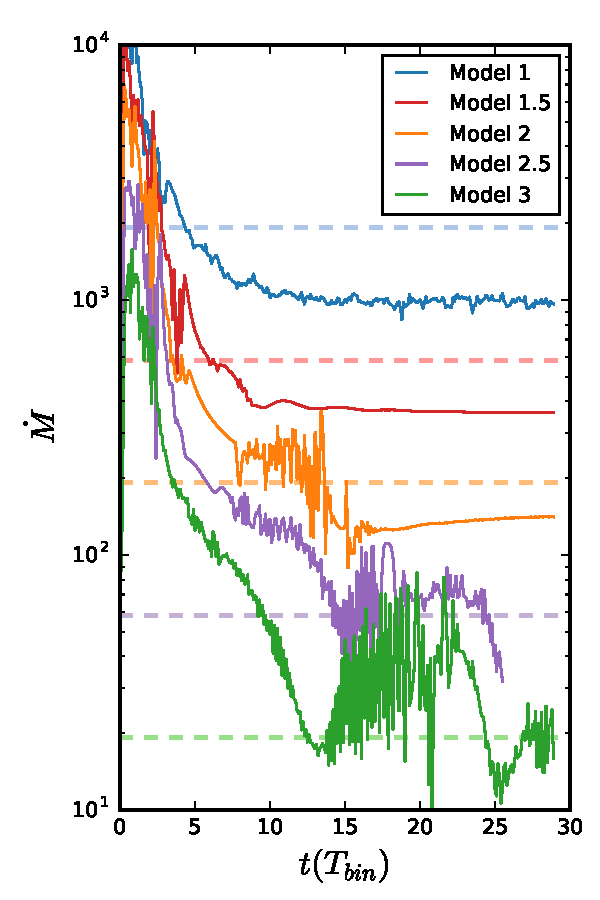
\includegraphics[width=0.8\textwidth]{figures/minidisk/mdot_all.pdf}
\end{center}
\caption{\figlabel{mdot_all} Accretion rate through the inner boundary as a function of time for \model{1} (blue), \model{1.5} (red), \model{2} (orange), \model{2.5} (purple), and \model{3} (green).  $\dot{M}_\text{nozzle}$ for each model is shown as a dashed line in the corresponding color. Variability lasts longer and is of greater amplitude in disks with lower accretion rates.  Models \texttt{1}, \texttt{1.5}, and \texttt{2} establish a quasi-steady state.}
\end{figure}

In \fig{tacc} we plot the accretion timescale $t_{\dot{M}} = M_\text{disk} / \dot{M}$ as a function of $\dot{M}$ for all primary models at the end of their runs.  The total disk mass $M_\text{disk}$ is calculated by integrating the lab-frame surface density $u^0 \Sig$ over the whole computational domain, and the accretion rates are taken from the inner boundary.  We see that Models \texttt{2.5} and \texttt{3} have accretion timescales longer than the runtime of the simulation, explaining the extended variability seen in \fig{mdot_all}.  A power-law fit to the data gives a slope of $-0.78 \pm 0.08$. This is of relevance to global Newtonian circumbinary accretion simulations, which typically employ a mass sink that removes some fraction of material every orbit.

\begin{figure}
\begin{center}
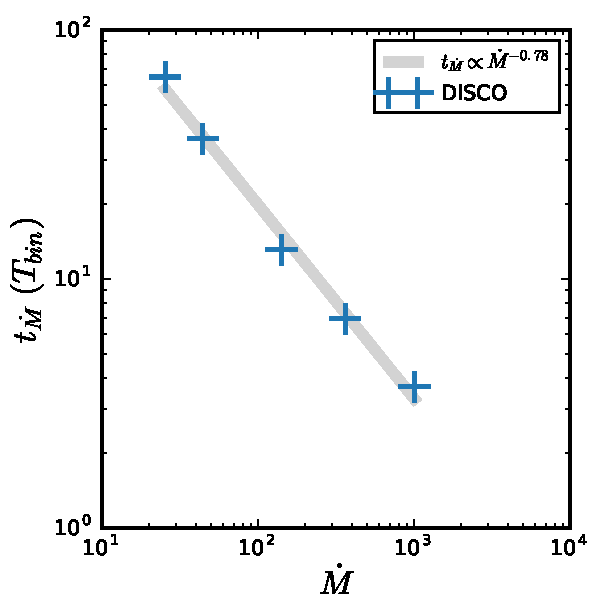
\includegraphics[width=0.8\textwidth]{figures/minidisk/tacc.pdf}
\end{center}
\caption{\figlabel{tacc} Accretion time $t_{\dot{M}}=M_\text{disk}/\dot{M}$ as a function of $\dot{M}$ for all models (blue plus signs), and power-law fit to the simulation data (gray line).  Models \texttt{1}, \texttt{1.5}, and \texttt{2} can accrete their entire disk mass within the run time of the simulation ($29 T_\text{bin}$) and achieve quasi-equilibrium, unlike Models \texttt{2.5} and \texttt{3} with lower accretion rates. The dependence of $t_{\dot{M}}$ on $\dot{M}$ follows a rough power law of $-0.78 \pm 0.08$.}
\end{figure}

\subsection{Wave Propagation}
\sectlabel{res-prop}

As a first diagnostic we check whether the two-armed spiral shocks adhere to the dispersion relation for tightly wound linear waves given by \eq{dispRelPitch}.  The shock detector (see \sect{shockDet}) returns the azimuthal coordinates of the leading $\Phi_{i,\text{lead}}(r)$ and trailing $\Phi_{i,\text{trail}}(r)$ edge of each shock $i=A,B$.  We consider the center of each shock $\Phi_i = (\Phi_{i,\text{lead}} + \Phi_{i,\text{trail}}) / 2$.  The pitch angle of a spiral $\Phi(r)$ is
\begin{equation}
	\tan \theta = -\frac{1}{r \Phi'(r)} \ . \eqlabel{deftanp} 
\end{equation}
We compute $\tan \theta_i$ for each shock according to \eq{deftanp} by performing a numerical centered difference on $\Phi_i(r)$.  At each radius we compute the average Mach number $\mathcal{M}$ as
\begin{align}
	\langle \mathcal{M} \rangle &=  \frac{|u|}{c_s / \sqrt{1-c_s^2}} \ , \\
	\text{where: } |u| &= \sqrt{\gamma_{\mu\nu} \langle u^\mu \rangle  \langle u^\nu \rangle} \nonumber \ .
\end{align}

In \fig{disp} we plot the pitch angle of shocks found in the minidisk simulations against the average Mach number of each annulus. We find good agreement between the numerically calculated pitch angles and the theoretical relationship $\eqrefp{dispRelPitch}$, indicating that the shocks propagate mostly in the linear regime.

\begin{figure}
\begin{center}
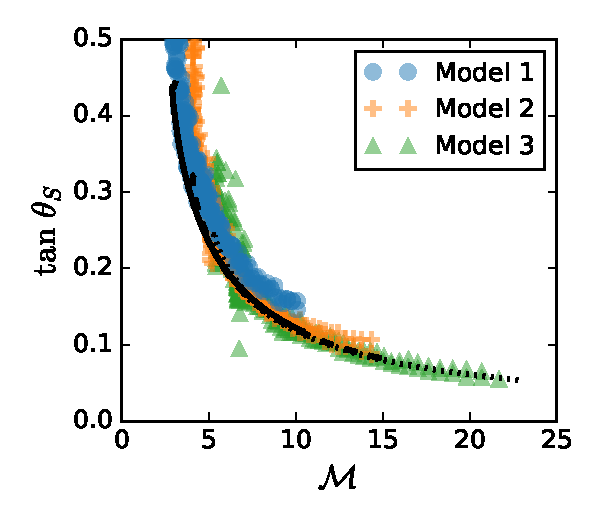
\includegraphics[width=0.8\textwidth]{figures/minidisk/q011_all_tanq_mach.pdf}
\end{center}
\caption{\figlabel{disp} Pitch angle versus average Mach number for \model{1} (blue circles), \model{2} (orange plus signs), and \model{3} (green triangles). Lines are the analytic prediction from the dispersion relation for tightly wound linear waves for \model{1} (solid), \model{2} (dashed), and \model{3} (dotted).  Spiral shocks propagate in a nearly linear regime, with better agreement at higher Mach numbers and lower accretion rates.}
\end{figure}


\subsection{Shock Dissipation}
\sectlabel{diss}

To quantitatively measure the coupling between the spiral shocks and the bulk disk flow, we measure the irreversible heating at each shock in post-processing.  Given the shock locations, we compute the jump in specific entropy $\Delta s_i = s_{i,\text{trail}} - s_{i,\text{lead}}$ over each shock at each radius.  To measure the specific irreversible heating over a shock of strength $\De s$ \cite{Rafikov16} defines the parameter $\psi_Q$ for a $\Gam$-law gas:
\begin{equation}
	\psi_Q \equiv \frac{1}{\Gam - 1} \left( e^{(\Gam -1)\De s } - 1 \right) \ . \eqlabel{def-psi}
\end{equation}
Then the specific irreversible heating at a shock is simply $T_\text{lead} \psi_Q$.  To determine the irreversible heating rate at a shock, the specific heating rate must be multiplied by the mass flux through the shock surface $\Phi(r)$.  When summed over all the shocks in an annulus, one gets the total irreversible heating rate:
\begin{equation}
	\dot{Q}_{irr} = \sum_i \left[ \Sigma \left(r u^\phi - r \Phi'(r) u^r \right) T \right]_{i,\text{lead}} \psi_{Q,i} \ . \eqlabel{QirrRaf}
\end{equation}

\fig{diss} shows the radial profiles of $\Delta s_i$, $\psi_{Q,i}$, $\avet{\dot{Q}_\text{irr}}$, and $\avet{\dot{Q}_{cool}}$ for \model{2} averaged from $20 T_\text{bin}$ to $29 T_\text{bin}$.  Note that $\avet{\dot{Q}_\text{irr}}$ does not include heating (cooling) due to adiabatic compression (expansion) and advection.  Both $\De s$ and $\psi_Q$ vary over an order of magnitude through the disk, reflecting the double-peaked radial distribution seen in \fig{sig-fid-28}. On average, $\psi_Q \sim 0.1$.  

The distribution of irreversible heating and cooling in \model{2} has a much smoother radial dependence than $\psi_Q$. The is reflective of the universal character of emission from thin accretion disks: the profile of $\avet{\dot{Q}_\text{cool}}$ for a steady axisymmetric thin disk subject to local dissipation depends only on the accretion rate and black hole parameters, not the particular form of the dissipation or opacities.  For comparison we plot the expected Novikov-Thorne $\avet{\dot{Q}_\text{NT}}$ using the asymptotic value of $\dot{M}$ from \fig{mdot-fid}. 

The heating and cooling are broadly similar over the extent of the disk, with $\avet{\dot{Q}_\text{irr}} \lesssim \avet{\dot{Q}_\text{cool}}$ most often.  Even in a steady state one would not expect them to match exactly, as some energy must be advected inwards.  Both $\avet{\dot{Q}_\text{irr}}$ and $\avet{\dot{Q}_\text{cool}}$ agree with the Novikov-Thorne profile in $12 M \lesssim r \lesssim 30M$ but far exceed it in the inner disk as $r \to r_\text{ISCO}$, peaking at $r \approx 7.5M$.

\begin{figure}
\begin{center}
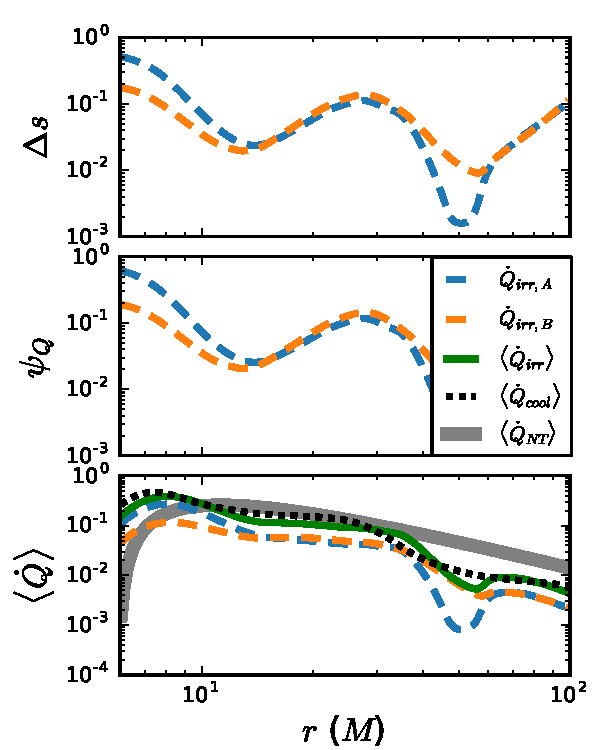
\includegraphics[width=0.8\textwidth]{figures/minidisk/q011_m3_diss_r.pdf}
\end{center}
\caption{\figlabel{diss} Radial profiles of dissipative shock quantities in \model{2}, time averaged from $(20 - 29) T_\text{bin}$.  Top to bottom: the entropy jump $\De s$, $\psi_Q$, and irreversible heating $\dot{Q}$. The shocks $A,B$ are plotted in blue and orange dashed lines, respectively.  The bottom panel also contains the total irreversible heating according to \eq{QirrRaf} (green solid line), the local cooling rate integrated over each annulus $\avet{\dot{Q}_\text{cool}}$  (black dotted line), and the same quantity from a Novikov--Thorne disk with $\dot{M} = 0.75 \dot{M}_2$ in gray.  Shock-dissipated heat is nearly balanced by radiative cooling and roughly follows the Novikov--Thorne profile until the inner $r\lesssim 10M$.}
\end{figure}

\subsection{Angular Momentum Transport}
\sectlabel{angmom}

Dissipation in the fluid flow is a sign of angular momentum transport and hence accretion. Indeed in every simulation we find that the accretion rate through the inner boundary (into the black hole) matched the accretion rate through the outer boundary (matter injection from the nozzle minus outflow).  A quasi-equilibrium, where the inner and outer accretion rates match, typically occurred within a few ($<10$) $T_\text{bin}$. 

The relative strength of stress in an accretion flow is typically measured by determining an effective Shakura--Sunyaev (or Novikov--Thorne) $\al$-parameter.  The gravitational forces of the companion, plus the global character of the shocks providing the dissipation, make $\al_{\text{eff}}$ a somewhat imprecise notion.  We present two measures of $\al_{\text{eff}}$.  First, following \cite{Ju16}, we calculate the $\al_{\dot{M}}$ required at each radius for a Novikov--Thorne disk of the same average temperature and accretion rate.  Second, \cite{Rafikov16} determines for shocked Newtonian disks $\al_{\dot{Q}} \sim \psi_Q / 3\pi$.  We take this same prescription without modification, as $\psi_Q$ is a scalar quantity and hence frame independent.  

The radial profiles of both $\al_{\dot{M}}$ and $\al_{\dot{Q}}$ are plotted in \fig{alpha} for the fiducial run.  We see that they are broadly similar across the disk, except near the ISCO at $r=6M$ where $\al_{\dot{M}}$ diverges owing to the singularity in the Novikov--Thorne model.

\begin{figure}
\begin{center}
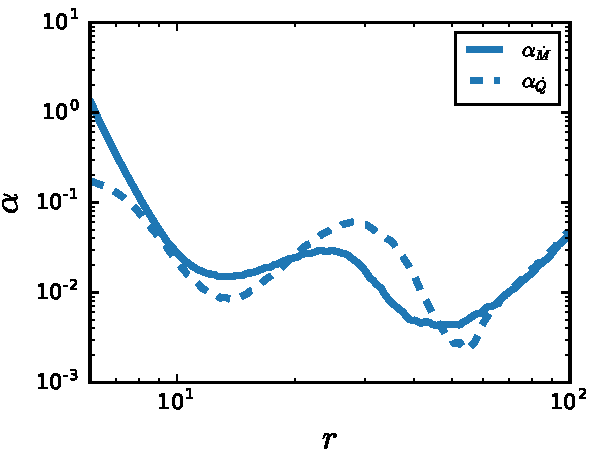
\includegraphics[width=0.8\textwidth]{figures/minidisk/q011_m3_alpha_r.pdf}
\end{center}
\caption{\figlabel{alpha} Radial profile of effective $\al$ parameters in \model{2} measured from the accretion rate $\al_{\dot{M}}$ (solid) and the local dissipation $\al_{\dot{Q}}$ (dashed).}
\end{figure}

To see the effect of the spiral shocks in detail, we decompose the torques acting on the disk according to \eq{angMomDecom} (see \sect{angMomDecom} for details). Each of the torques $\tau_{\dot{M}}$, $\tau_\text{Re}$, $\tau_\text{ext}$, and $\tau_\text{cool}$ can be measured directly from \Disco{} output.  The Reynolds torque $\tau_\text{Re}$ in particular measures the angular momentum transport due to nonaxisymmetric features.  One can estimate the torque due to spiral shocks from $\psi_Q$ directly \citep{Rafikov16}:
\begin{equation}
	\tau_\text{shock} = \frac{\dot{Q}_\text{irr}}{v^\phi - \Om_P} \ . \eqlabel{tauRaf}
\end{equation}
If angular momentum transport in minidisks is completely due to shocks, $\tau_{shock}$ should match $\tau_{Re}$.

Alternately, one can ask what sort of local angular momentum flux could account for the accretion and shock heating in an azimuthally averaged sense (such as an $\al$-viscosity).  Such a flux would be an addition $t^{\mu\nu}$ to the gas stress energy tensor.  Assuming, like the viscous stress tensor, $u_\mu t^{\mu\nu}_{non-id} = 0$ the energy and angular momentum conservation equations are modified to
\begin{align}
	&\partial_t \ave{\Sig \eps u^\mu} + \partial_r \ave{\Sig \eps u^r} = \ave{\Pi \nabla_\mu u^\mu} - \dot{Q}_\text{cool} + \ave{t^{\mu\nu} \nabla_\mu u_\nu} \ ,\\
	&\partial_t \ave{\Sig h u^0 u_\phi + t^0_\phi} + \partial_r \ave{\Sig h u^r u_\phi + t^r_\phi} = \ave{f_\phi} \ .
\end{align}
Identifying $\ave{t^{\mu\nu} \nabla_\mu u_\nu} \sim \ave{t^r_\phi \partial_r u^\phi}$ with $\ave{\dot{Q}_\text{irr}}$, one gets the relation
\begin{equation}
	\tau_{t} = \partial_r \ave{t^r_\phi} \approx \partial_r \left(\frac{\dot{Q}_\text{irr}}{\ave{\partial_r u^\phi}} \right)\ . \eqlabel{tauLoc}
\end{equation}
Such a local model neglects the global structure of spiral shock waves but may be interesting on the basis of comparison,  especially since it is the root of the $\alpha$-prescription.

We compare the predicted torque due to spiral shocks given in \eq{tauRaf} to the measured $\tau_\text{Re}$ and $\tau_{\dot{M}}$ for the minidisk models in Figures \figref{torque-m2}, \figref{torque-m3}, and \figref{torque-m4}.  The measured torques are calculated by azimuthally integrating grid quantities and centered differencing in $r$ when necessary.  The predicted torques due to irreversible shock heating, on the other hand, are calculated directly from the entropy jump $\De s$ measured to calculate $\psi_Q$.  

\model{1} is very near a steady state, with the accretion torque $\tau_{\dot{M}}$ balanced by $\tau_\text{Re}$, $\tau_\text{ext}$, and $\tau_\text{cool}$ throughout the $r < 100M$ region.  The small contribution of $\tau_\text{ext}$ and $\tau_\text{cool}$ to the torque balance indicates that the bulk of the angular momentum transport is provided by $\tau_\text{Re}$, a fact also true in Models \texttt{2} and \texttt{3}.  This alone indicates the non-axisymmetric structures drive accretion in these disks.  The discrepancy in the balance between $\tau_{\dot{M}}$ and $\tau_\text{Re}$ increases in \model{2} and again in \model{3}, indicating these disks are in much less steady states.  In \model{3} they widely differ, and there is even a narrow region undergoing deccretion.  

The shock torque model $\tau_\text{shock}$ shows good agreement with $\tau_\text{Re}+\tau_\text{ext}$, especially for Models \texttt{1} and \texttt{2} where it deviates by at most $30\%$ in $r < 60M$.  Even \model{3}, which is still evolving strongly in time, shows $\tau_\text{irr}$ agreeing well outside the band $40M \lesssim r \lesssim 50M$.  We find the local dissipation model $\tau_t$ does a poor job of predicting the torque on the disk.

\begin{figure}
\begin{center}
	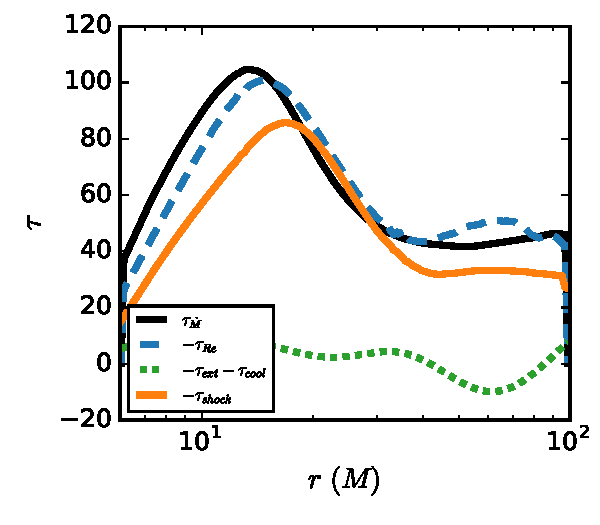
\includegraphics[width=0.8\textwidth]{figures/minidisk/q011_m2_torque_r.pdf}
\end{center}
	\caption{\figlabel{torque-m2} Time-averaged accretion torque $\tau_{\dot{M}}$ (black solid line), Reynolds torque $\tau_{Re}$ (blue dashed line), external and cooling torques $\tau_{ext}+\tau_{cool}$ (green dotted line), and predicted torque from spiral shocks $\tau_{irr}$ (\eq{tauRaf}; orange solid line) for \model{1}. Time averaging was over $(20-29)T_\text{bin}$.  The predicted shock torques $\tau_\text{shock}$ follow the trend of the Reynolds torque $\tau_\text{Re}$.}  
\end{figure}

\begin{figure}
\begin{center}
	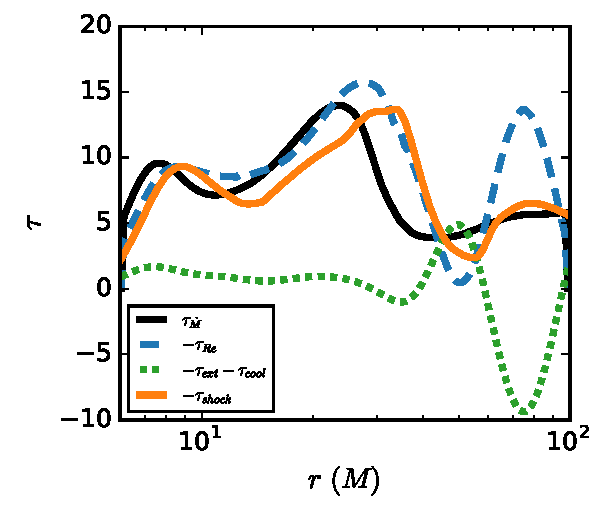
\includegraphics[width=0.8\textwidth]{figures/minidisk/q011_m3_torque_r.pdf}
\end{center}
	\caption{\figlabel{torque-m3} Same as \fig{torque-m2}, but for \model{2}}  
\end{figure}

\begin{figure}
	\begin{center}
	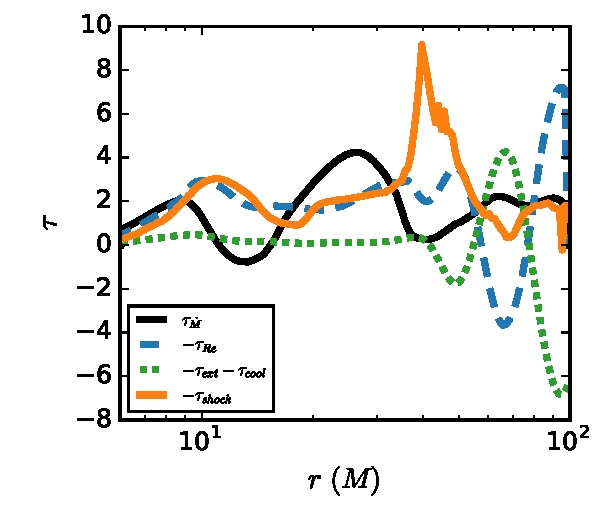
\includegraphics[width=0.8\textwidth]{figures/minidisk/q011_m4_torque_r.pdf}
	\end{center}
	\caption{\figlabel{torque-m4} Same as \fig{torque-m2}, but for \model{3}}  
\end{figure}

\subsection{Spectral Comparison to Novikov--Thorne}
\sectlabel{spectra}

As seen in \fig{diss} the rate of cooling in the inner disk $r < 10M$ is in significant excess to the standard Novikov--Thorne model.  This naturally leads to the question as to whether there is an observational difference between a standard thin disk and one undergoing shock-driven accretion.  We calculate the observational spectrum of each model using the ray-tracing methods of \sect{raySpec}, based on the method of \cite{Kulkarni11}.

\begin{figure*}
	\begin{center}
	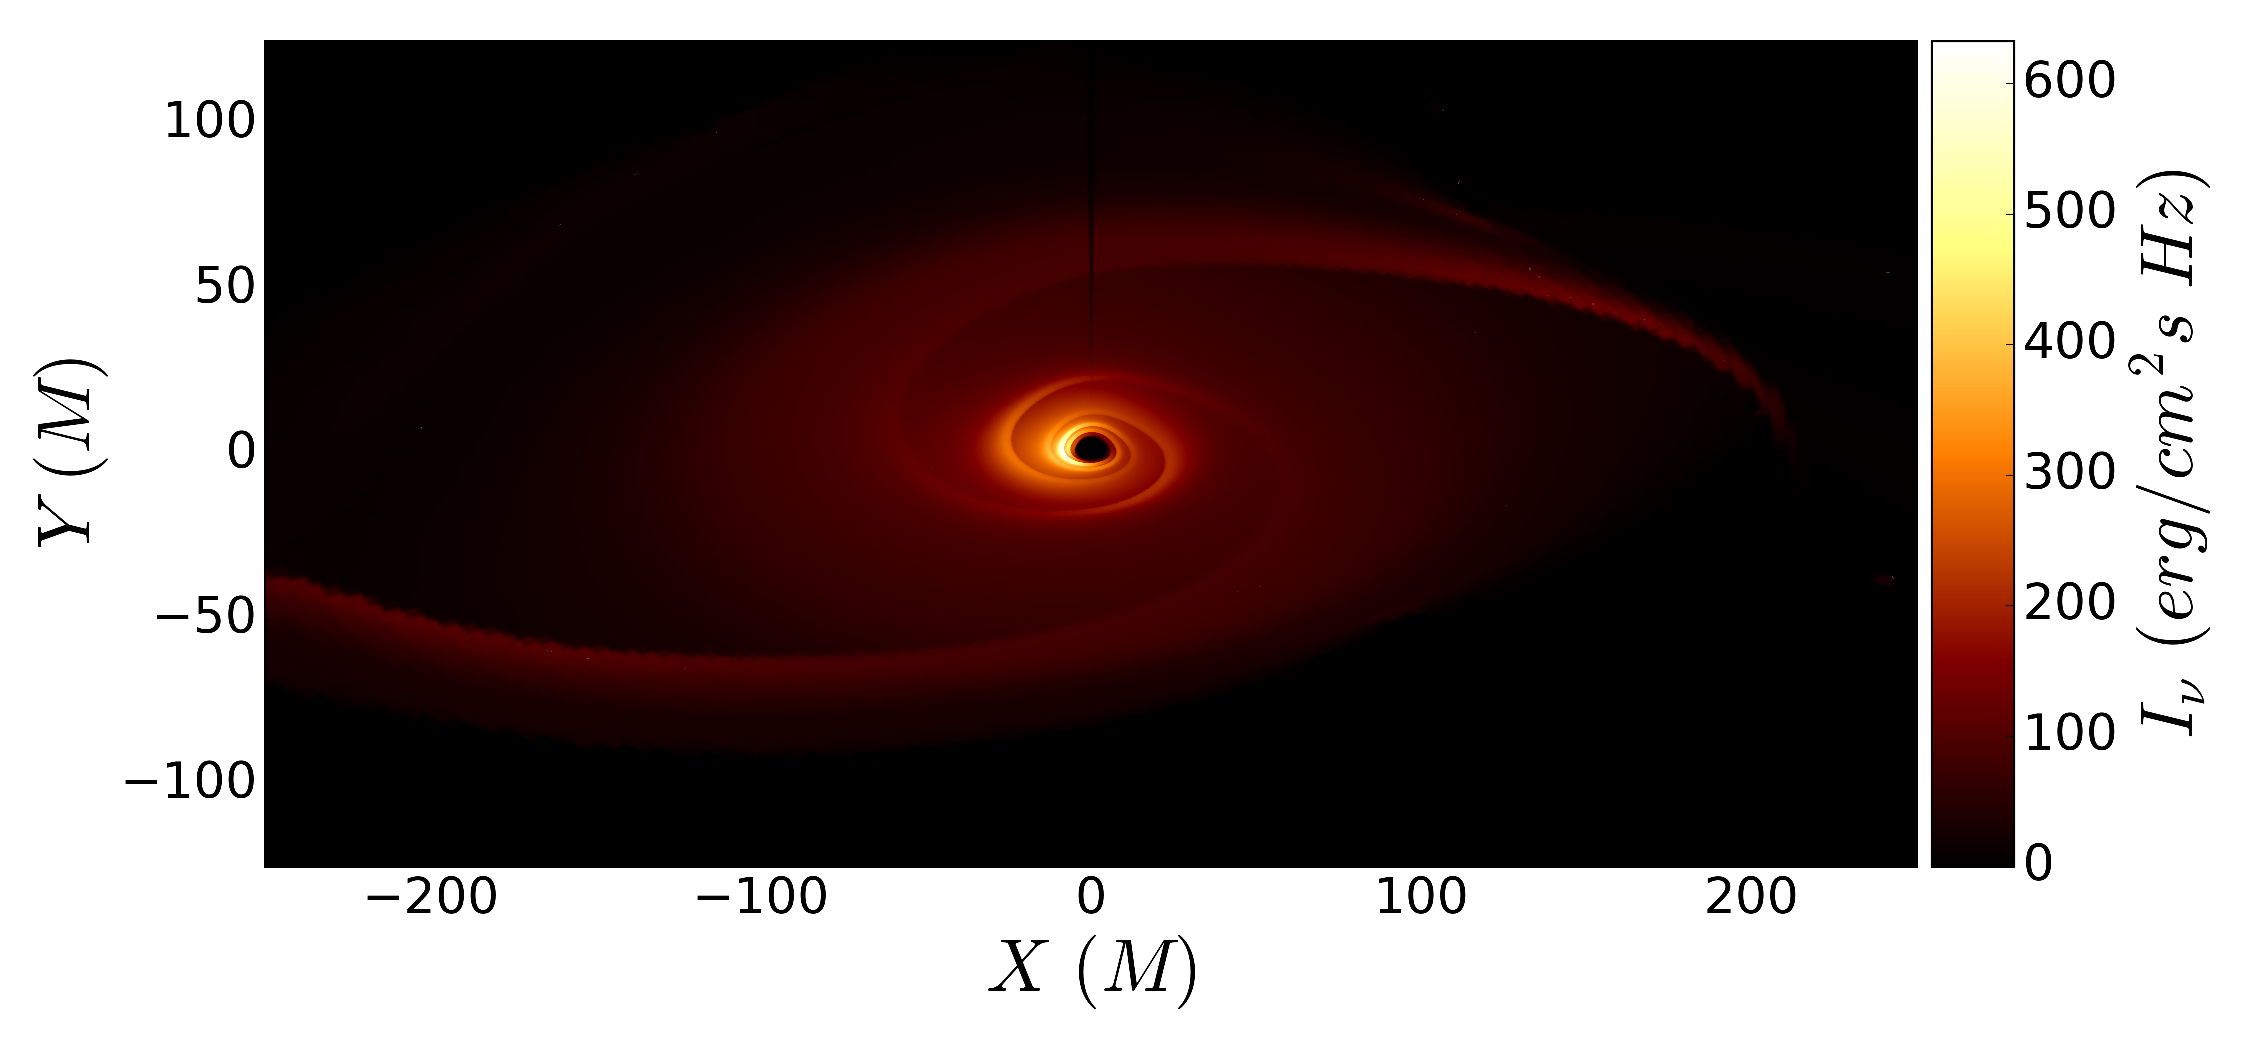
\includegraphics[width=0.8\textwidth]{figures/minidisk/q011_m3_im.pdf}
	\end{center}
	\caption{\figlabel{im} Ray-traced image of \model{2} at $\nu =   1$ keV. Shocks are clearly visible even near the black hole's shadow.  Relativistic beaming increases the intensity of observed emission in material with velocities toward the observer.}
\end{figure*}

An image of the specific intensity $I_{0.1\text{ keV}}$ for \model{2} at $t=28 T_\text{bin}$ viewed at inclination $i=60^\circ$ is shown in \fig{im}.  The total emission is dominated by the bright inner region, and the two-armed structure is clearly visible. We generate the spectrum by integrating over such images at several frequencies.  The spectrum corresponding to \fig{im} is shown in \fig{spec}. 

The spectrum of each model at $28 T_\text{bin}$ is plotted in \fig{spec} with reference Novikov--Thorne curves.  Each spectrum is calculated including only the region $r<40M$, to ease comparison with the Novikov--Thorne model and between models by removing the effect of variable outer disk truncation.  Each Novikov--Thorne spectrum is calculated using the corresponding model's accretion rate at the inner boundary, time averaged over $(20-29)T_\text{bin}$.  In this comparison all model spectra are well characterized by the Novikov--Thorne spectrum, except for a slight excess at $\nu > 10$ keV.  This excess is precisely due to the large cooling rate at $r<10M$ seen in \fig{diss}, and corresponds to the presence of shock-heated gas near and within the ISCO.  

\begin{figure*}
	\begin{center}
	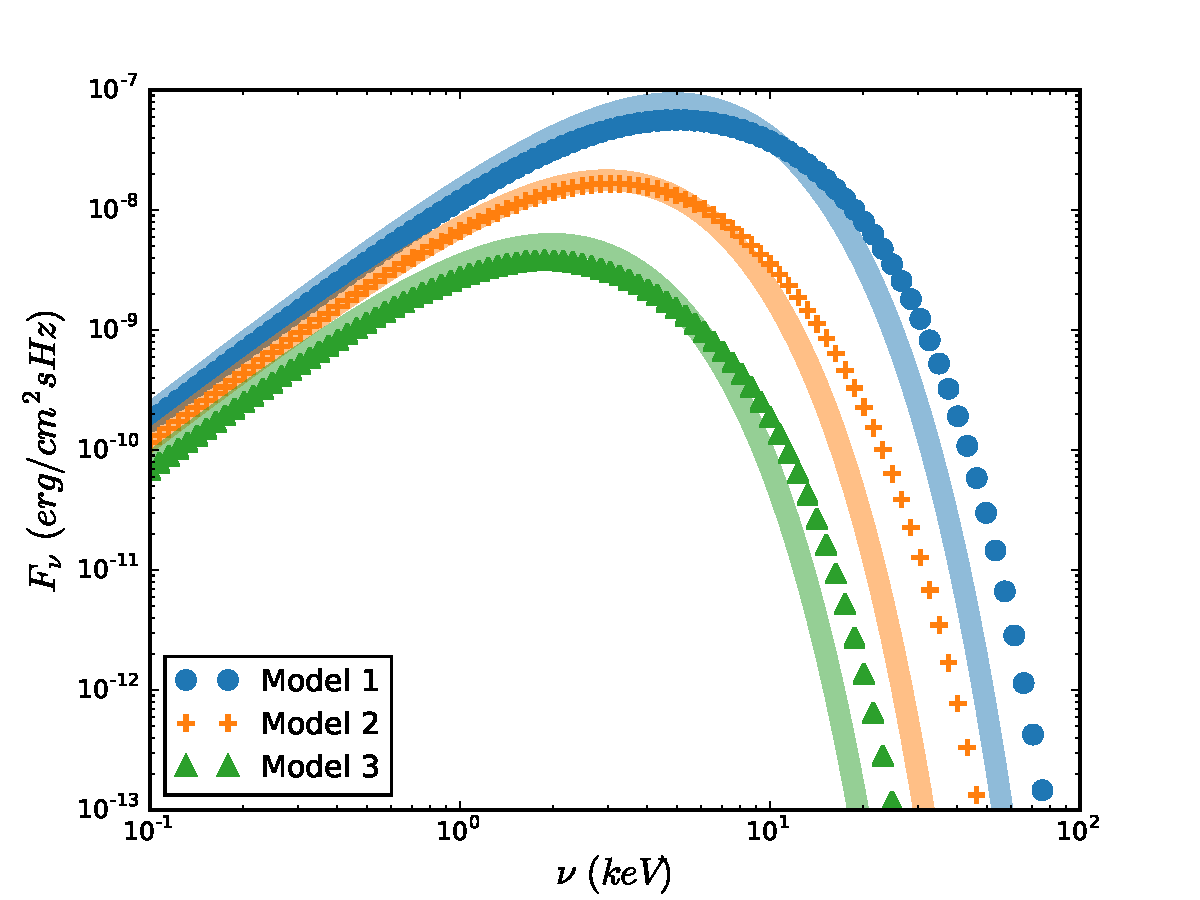
\includegraphics[width=0.8\textwidth]{figures/minidisk/q011_spec_all.pdf}
	\end{center}
	\caption{\figlabel{spec} Spectra of \model{1} (blue circles), \model{2} (orange plus signs), and \model{3} (green triangles) at $t = 28 T_\text{bin}$, obtained by integrating over the ray-traced intensity (e.g. in \fig{im}).  Solid lines are Novikov--Thorne spectra with $\dot{M}$ of the inner boundary averaged over $20 T_\text{bin}$ to $29 T_\text{bin}$ for each model.  Only the $R<40M$ region is included in the integration, to remove the effect of truncation at the outer disk edge.  The inclination angle $i=60^\circ$ and the distance $D=1$ kpc.  The data are consistent with the Novikov--Thorne profile at low energies but show a high-energy excess, consistent with the increased shock dissipation and radiative cooling observed at $r\lesssim 10M$.}
\end{figure*}

\subsection{Dependence on Inner Boundary Condition}
\sectlabel{bc}

Accretion onto a black hole has a well-defined physical inner boundary condition given by the event horizon.  This is advantageous for numerical studies, as it leaves no choices for the investigator. Simply extend the numerical grid through the horizon, and the metric will prevent any information about the inner edge of the grid from propagating outward into the observable simulation volume.  

Unfortunately, due to the CFL condition, this puts a heavy penalty on the time step for the hydro evolution.  Gas near the horizon plunges radially inward at almost the speed of light, so to capture the fastest modes in an explicit time evolution scheme, the time step must essentially be light limited. This makes long time evolution very computationally expensive and reduces the advantage of the azimuthal mesh motion in \Disco{}.

To evolve for several binary orbits, we find it necessary to move the inner boundary of the numerical grid to $r=4M$, above the event horizon.  The choice of $4M$ was made deliberately, as this is inside the sonic radius of the flow. Inside the sonic radius characteristics are all directed inward and the upwinded hydrodynamic evolution scheme prevents information from propagating outward.  This gives the same advantages as including the event horizon on the grid, but with a far smaller time step penalty.  The inner boundary condition within $4M$ is cold, isentropic inflow and matches the exterior solution very well.

To verify that our boundary condition does not affect the global evolution, we mapped the \model{2} solution at $t=25 T_\text{bin}$ onto a new grid that does extend within the horizon.  This grid has $r_\text{min} = 1.8M$, and is referred to as \model{2-bc}.  We evolve \model{2-bc} for a single orbit, to $26T_\text{bin}$.  The azimuthally averaged surface density and radial velocity profiles of \model{2} and \model{2-bc} are shown in \fig{bc_hr_comp}.  The \model{2-bc} curves match those of \model{2} and smoothly continue through the horizon at $R=2M$.  This demonstrates the effectiveness of the isentropic inner boundary condition, even when placed above the horizon.

\begin{figure}
	\begin{center}
	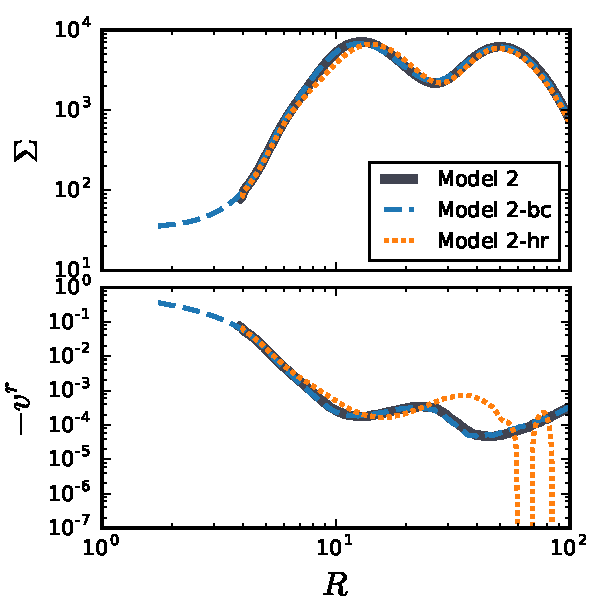
\includegraphics[width=0.8\textwidth]{figures/minidisk/q011_bc_hr_comp.pdf}
	\end{center}
	\caption{\figlabel{bc_hr_comp} Azimuthally averaged lab-frame surface density $\Sigma$ and radial velocity $\ave{v^r}$ for \model{2} at $29T_\text{bin}$ (solid gray line), \model{2-bc} at $26T_\text{bin}$ (dashed blue line), and \model{2-hr}  at $32T_\text{bin}$ (dotted orange line). \model{2-bc} smoothly continues \model{2} into the horizon even after an orbit of time evolution, indicating the robustness of the inner boundary condition.  The high-resolution \model{2-hr} develops time variability that does not settle down over the duration of the simulation, but the overall density distribution agrees well.}
\end{figure}

\subsection{Numerical Resolution}
\sectlabel{res}

To investigate the effects of numerical resolution, we mapped Model 2 at $t=28T_\text{bin}$ to a grid with double the resolution, 512 logarithmically spaced radial zones.  The simulation was run for four binary orbits, to $t = 32 T_\text{bin}$, and is denoted Model \texttt{2-hr}.

Model \texttt{2-hr} retains the strong two-armed shock structure. A similar clumpy accretion behavior develops as in the early evolution of \model{2} (between $8$ and $17$ $T_\text{bin}$, see \sect{fiducial}).  The remapping procedure upsamples the \model{2} grid, necessarily producing some small--scale noise.  This may be sufficient to push the model out of the quasi-equilibrium found by \model{2}. The clumpy accretion persists the length of the simulation, making a direct comparison between \model{2} and \model{2-hr} difficult.

The azimuthally averaged lab-frame surface density and radial velocity for \model{2-hr} are also plotted in \fig{bc_hr_comp}.  The data are from $t = 32T_\text{bin}$, where it appears that the clumpy accretion is beginning to settle down.  The unsteady nature of the flow is demonstrated in the radial velocity, where two regions can be seen with net positive velocity.  These fluctuations have little effect on the density distribution, which remains in good agreement with \model{2}.


%%%%%%
% Discussion %
%%%%%%

\section{Discussion}
\sectlabel{discussion}

We have studied the accretion dynamics onto a black hole in a binary system being fed by a circumbinary disk using 2D GRHD simulations. We have demonstrated the effectiveness of spiral shocks at driving accretion in these black hole ``minidisks,'' in broad agreement with recent Newtonian simulations in the context of CVs \citep{Ju16}  and circumplanetary disks \citep{Zhu16}.  The primary additions of this work are confirming the presence of shock-driven accretion when the disk is dynamically cooled, demonstrating that tidally driven spiral shocks can propagate throughout the disk and into the ISCO, enhancing emission of soft X-rays above the Novikov--Thorne model, and numerically verifying in the general relativistic case the relationship between disk torque and shock dissipation predicted by \cite{Rafikov16} for Newtonian disks.

We expect important aspects of our 2D simulations to carry over to the 3D case, though fully 3D GR(M)HD simulations of minidisks remain a topic for future study.  Analytic work has demonstrated that, while some wave modes are refracted out of the disk by the expected vertical temperature gradients, other modes will be channeled and amplified by the same gradients \citep{Lubow98}. \cite{Ju16} performed a single Newtonian 3D magnetohydrodynamic (MHD) simulation of a CV disk, where strong spiral shocks were clearly present and provided comparable torque to the MHD turbulence.  \cite{Bae16} performed a suite of Newtonian 3D disks, isothermal and adiabatic, subject to an $m=2$ perturbing potential.  They found all spiral waves were subject to an instability that disrupted the wave and generated turbulence.  The strength of the instability depended sensitively on the thermodynamics of the disk.

Clearly more work needs to be done to determine the role tidally induced spiral shocks play in accretion disks, both relativistic and nonrelativistic.  The results of \cite{Ju16}, \cite{Zhu16}, and \cite{Bae16} seem to indicate that spiral shocks can be dynamically important, either working in concert with the MRI and essentially providing a lower bound on $\al$, or by seeding turbulence directly.  The sensitive dependence on thermodynamics indicates that their ultimate role will be highly dependent on the cooling mechanisms and equations of state of the material at hand.

In black hole disks, if the shocks propagate undisturbed, they can provide dissipation at the ISCO, leading to a high-energy radiative excess over the standard Novikov--Thorne models.  This may be relevant for spin measurements of black hole X-ray binaries that rely on continuum fitting. Three-dimensional GRMHD simulations have also found MRI dissipation within the ISCO and conclude that continuum fitting based on Novikov--Thorne may mildly overestimate spins \citep{Penna10, Noble10, Kulkarni11, Schnittman15}.  A recent report raises the possibility of a shock in the outer, optically emitting region of LMC X-3 but found no similar evidence in the X-ray data \citep{Steiner14}.

Of relevance to SMBH binary detection, our results confirm that the minidisk SED resembles a standard disk blackbody apart from the high-energy excess (\fig{spec}).  Minidisks are soft X-ray sources undergoing orbital motion at potentially relativistic velocities.  In the Earth's frame, relativistic beaming will induce a periodic variation in each minidisk's emission that should be absent in the emission from the global circumbinary disk \citep{DOrazio15}.  Discriminating the minidisk emission from the circumbinary disk may be possible if the SED of the entire system has a ``notch,'' as suggested in \cite{Roedig14}.  However, global Newtonian simulations with \Disco{} show that gas thrown off the minidisks can impact and shock-heat the cavity wall, creating hot spots that can smooth the spectrum \citep{Farris15A}.

Emission of GWs shrinks the orbit of the binary, leading to merger in a time given by \eq{Tmerge}, thousands of orbits for the parameters in this work.  We find that spiral shock patterns establish themselves very rapidly, in less than a single orbit of the binary, and can lead to a quasi-steady state in dozens of binary orbits.  This separation of timescales implies that spiral shocks will remain in quasi-steady state and drive accretion as the binary orbit secularly evolves.  This should remain the case until the binary begins evolving on an orbital timescale, when the separation is tens of $M_\text{bin}$. In this regime our quasi-Newtonian treatment of the binary potential ceases to be valid and a fully general relativistic binary black hole metric should be employed as in \cite{Farris12,Noble12,Zilhao15}.

After the LIGO discovery of GW150914 and GW151226, electromagnetic counterparts to stellar mass black hole binaries are of great interest \citep{LIGO16GW150914Discovery, LIGO16GW151226}.  If a black hole binary exists in a gaseous environment, for instance, within an AGN disk \citep{Bartos16, Stone17} or post-supernova fallback \citep{Perna16}, it will undergo circumbinary accretion and minidisks will form, potentially producing distinct radiative signatures.  


%%%%%%
% Summary %
%%%%%%

\section{Summary}
\sectlabel{summary}


We performed general relativistic hydrodynamical simulations of accretion disks in the Schwarzschild metric subject to tidal forces of a binary companion.  These disks, referred to as ``minidisks,'' were fed from a nozzle at the L2 Lagrange point, modeling the accretion streams feeding minidisks seen in circumbinary accretion simulations.  The tidal forces excited two-armed spiral shock waves that propagate throughout the disk,  generating heat through dissipation, transporting angular momentum, and efficiently driving accretion into the black hole.

The spiral shocks propagate primarily in the nearly linear regime, agreeing with the relativistic generalization of the WKB dispersion relation for tightly wound linear waves.  Measurements of the jump in specific entropy across the spiral shocks provide a measure of the irreversible heating of the disk.  The cooling profile qualitatively follows the Novikov--Thorne profile in the outer disk but maintains a significant excess of emission within $r \lesssim 10 M$.  The angular momentum transport in all models is driven by the Reynolds stress due to the spiral shocks, in agreement with the shock-driven torque model of \cite{Rafikov16} to within $\sim30\%$.  The stress corresponds to an effective Shakura--Sunyaev $\al$-parameter on the order of a few$\times 10^{-2}$.

Accretion via spiral shocks is a purely hydrodynamical effect, occurring without the need for magnetic fields or radiation.  Any disk in a binary system will be subject to tidal forces, and the ensuing spiral shocks can carry a non-negligible portion of the angular momentum transport budget.  Spiral shocks can propagate through the ISCO and may provide an emission excess over the standard Novikov--Thorne models.

\section{Chapter Acknowledgements} \sectlabel{acknowledgements}
We are grateful to Patrick Cooper, Dan D'Orazio, Paul Duffell, Brian Farris, Andrei Gruzinov, Zoltan Haiman, and Roman Rafikov for many useful conversations.  This work was supported in part by NASA through Astrophysics Theory (ATP) Grant NNX11AE05G.  Computations were performed on the Pleiades cluster at NASA AMES and on the Ria cluster at the Center for Cosmology and Particle Physics, New York University.

\renewcommand{\chapid}{scalefit}

% Chapter specific commands:

\newcommand{\scalefit}{{\texttt{ScaleFit}}}
\newcommand{\boxfit}{{\texttt{BoxFit}}}
\newcommand{\ramcode}{{\texttt{RAM}}}
\newcommand{\blastcode}{{\texttt{BLAST}}}
\newcommand{\ram}{{\texttt{RAM}}}
\newcommand{\emcee}{{\texttt{emcee}}}
\newcommand{\multinest}{\texttt{MultiNest}}
\newcommand{\afterglowlibrary}{{\texttt{http://cosmo.nyu.edu/afterglowlibrary/}}}

% Math:

\newcommand{\ddl}{d_{L,28}}
\newcommand{\Eiso}{E_{iso}}
\newcommand{\Edl}{E_{iso, 53}}
\newcommand{\ndl}{n_{0, 0}}
\newcommand{\thO}{\theta_0}
\newcommand{\thobs}{\theta_{obs}}
\newcommand{\epse}{\epsilon_e}
\newcommand{\epsB}{\epsilon_B}
\newcommand{\xN}{\xi_N}
\newcommand{\tobs}{t_{obs}}
\newcommand{\Fp}{F_{peak}}
\newcommand{\cf}{\mathfrak{f}}
\newcommand{\cfp}{\cf_{peak}}
\newcommand{\cfm}{\cf_{m}}
\newcommand{\cfc}{\cf_{c}}
\chapter{Scalefit \chaplabel{scalefit}}

This \paper\ is joint work with Hendrik van Eerten (Bath), Andrew MacFadyen (NYU), and Bin-Bin Zhang (University of Alabama) published in \emph{The Astrophysical Journal} as \citet{Ryan15}.

\section{Chapter abstract}

We constrain the jet opening angle and, for the first time, the off-axis observer angle for gamma-ray bursts in the \swiftXRT{} catalogue by using the \scalefit{} package to fit afterglow light curves directly to hydrodynamic simulations.
The \scalefit{} model uses scaling relations in the hydrodynamic and radiation equations to compute synthetic light curves directly from a set of high resolution two-dimensional relativistic blast wave simulations.  The data sample consists of all \swiftXRT{} afterglows from 2005 to 2012 with sufficient coverage and a known redshift, 226 bursts in total.  We find the jet half-opening angle varies widely but is commonly less than 0.1 radians.  The distribution of the electron spectral index is also broad, with a median at $2.30$. 
We find the observer angle to have a median value of 0.57 of the jet opening angle over our sample, which has profound consequences for the predicted rate of observed jet breaks and affects the beaming corrected total energies of gamma-ray bursts.

%%%%%%%%%
% Introduction  %
%%%%%%%%%

\section{Introduction}


Gamma-ray bursts (GRBs) are intense flashes of gamma-rays believed to be caused by collapsing massive stars and merging compact binaries \citep{Woosley93, MacFadyen99, Eichler89}.  First observed by the \vela{} satellites in 1969, GRBs occur isotropically in the sky and persist for as long as several minutes or as short as fractions of a second \citep{Klebesadel73}.  In 1997 the \bepposax{} satellite detected a faint, decaying X-ray signal from GRB 970228 following the gamma-ray emission \citep{Costa97}.  Dubbed the GRB \emph{afterglow}, similar emission was detected in several subsequent GRBs.  Optical components to the afterglow were soon observed \citep{Groot97}.  Spectra from these optical components allow redshifts to be determined, which place the progenitors of GRBs at cosmological distances from Earth \citep{Metzger97}.  

The short timescale of a GRB indicates the radiation most likely is emitted by a compact object, such as a collapsing stellar core or merging neutron star binary.  If the progenitor were to radiate isotropically, it would have to radiate away a significant amount of its rest-mass energy to be visible from Earth.  Given the required radiative efficiency of such a process, this seems extremely unlikely.  Rather the radiation is most likely emitted in a collimated fashion; as a jet directed towards Earth.  The afterglow arises when the jet begins to propagate into the medium surrounding the burst (the circumburst medium).  The subsequent expansion into the cold surrounding gas creates a relativistic blast wave propagating out from the progenitor.  Electrons in the gas emit synchrotron radiation as they are accelerated by the magnetic fields in the forward shock.  Relativistic beaming collimates the radiation in the direction of jet propagation, which is observed on Earth as the afterglow.  The early afterglow is visible across the electromagnetic spectrum, from radio to X-ray.  As the blast wave expands and cools over the course of months the higher frequencies fade away, radio emission can continue for a year after the burst until it too drops below observational sensitivity.  This basic afterglow picture was first outlined in the fireball model \citep{Rees92}, but is a natural consequence of any GRB engine which deposits sufficient energy into the circumburst medium.  Although the precise mechanics of GRB engines are still uncertain, the relatively simpler physics of afterglows opens them up to direct simulation and analysis.

The relativistic jet-like nature of the blast wave leads to some immediate geometric conclusions.  At early emission times, only a small patch on the leading edge of the blast wave is visible.  As time goes on, more and more of the blast wave becomes visible to the observer.  This effect slows the temporal decay of the afterglow.  However, after a long enough time, the entire blast wave becomes visible, and the afterglow will decay faster.  Further steepening of the afterglow light curve is caused by hydrodynamic spreading of the blast wave as it decelerates.  The steepening due to these processes is called the \emph{jet-break}, and is an ubiquitous effect of relativistic collimated emission.  Current observations of afterglow light curves see far fewer jet-breaks than expected, this is known as the missing jet-break problem \citep{Sato07,Liang08, Kocevski08, Racusin09}.

The jet orientations are randomly distributed for cosmologically distant sources such as GRBs. \citet{vanEer10offaxis, vanEer11} show that observing an afterglow from an observer angle comparable to the jet opening angle, as opposed to straight-on, can smear out the jet-break and delay the full transition until after \swift{} ceases observations. This provides a plausible resolution to the missing jet-break problem.  A sufficiently detailed model capable of predicting distinct light curves for off-axis observers should, in principle, allow the observer angle $\thobs$, the direction of the outflow relative to Earth, to be measured from afterglow data. With enough data, this information can be used to revise predictions for the rate of jet-breaks observed by \swift{} (or other instruments), by revealing the extent to which observational biases will alter the intrinsic random distribution of source directions.

The hydrodynamics of a collimated outflow are inherently multi dimensional.  Calculating an afterglow light curve from basic physical parameters of the blast (such as the explosion energy, opening angle, and observer angle) requires numerical simulation since there is no known exact solution to the two-dimensional blast wave.  However, since state-of-the-art numerical simulations typically take days to run, using them directly in the analysis of data usually requires either approximations or significant amounts of computer time.  The \boxfit{} package addressed this problem with a two-fold approach \citep{vanEer12boxfit}.  Using the scale-invariance between blast energies and circumburst medium densities, fully time dependent hydrodynamical data can be generated for arbitrary values of these parameters from only a single hydrodynamics simulation.  Strong compression of the simulation output allow for data from a large sample of opening angles to be loaded into memory simultaneously.  \boxfit{} is able to generate light curves on the fly by only running a radiative transfer code using the compressed hydrodynamics data, reducing the generation time from days to seconds.  The \scalefit{} analysis code \citep[][in prep]{vanEer14scalefit} used in this work goes a step further, making use of scaling relations in the radiation equations to generate light curves directly from a precomputed table of spectral parameters \citep{vanEer12scale}.  Using \scalefit{}, an afterglow light curve can be generated directly from high resolution simulations in milliseconds. 

We make use of the speed up to perform a Markov chain Monte Carlo (MCMC) curve fitting procedure on a large sample of afterglows observed by the \swift{} X-Ray Telescope (\swiftXRT{}).  The procedure to fit a single burst requires about ten million light curves to be generated with distinct parameters, and takes a couple of hours on a standard workstation.  Any detailed model with multiple parameters is likely to exhibit degeneracies between parameters when performing a fit in only a single band.  Degenerate parameters exhibit high correlations with each other but are individually unconstrained by the data.  An advantage of the Bayesian MCMC approach is the ability to treat degeneracies as \emph{nuisance parameters}.  Nuisance parameters may be marginalized over, incorporating their uncertainties into a probability distribution for only the parameters of interest.  To efficiently sample the parameter space we use the parallel tempered affine invariant ensemble sampler \citep{Goodman10} implemented by the \emcee{} package \citep{emcee}.  While our final results leave several model parameters unconstrained, this uncertainty is folded into the estimates for the parameters we can constrain well: the jet half opening angle $\thO$, the off-axis observer angle $\thobs$, and the electron spectral index $p$.  Details of the \scalefit{} model, its implementation, and a public release of the code will be given in a forthcoming paper \citep[][in prep]{vanEer14scalefit}.  This paper focuses on the results of using \scalefit{} on the \swiftXRT{} dataset.  

In section 2 we give an overview of the \scalefit{} afterglow model and the simulations upon which its based.  Section 3 discusses the \swiftXRT{} data sample, and section 4 details the specific analysis we perform.  We find bursts exhibit a wide range of opening angles, but most commonly have a half-opening angle $\thO < 0.1$ rad.  The distribution of electron spectral index $p$ favours $p\sim2.3$.  The off-axis observer angle tends to be around 0.6 of the half opening angle.  The results are summarized in section 5 and discussed in section 6, with specific fit results given in the appendix.  A subset of these results were presented in \cite{Ryan13}.

%%%%%
%Section 2 - Model
%%%%%

\section{The Model}

The \scalefit{} GRB afterglow model uses a series of high resolution hydrodynamic simulations to calculate the time evolution of the afterglow spectral parameters.  From these parameters we extract a set of scale-invariant characteristic quantities.  The characteristic quantities depend only on $\thO$, the opening angle of the jet producing the afterglow, $\thobs$, the angle at which the observer is off-axis (the observer angle), and observer time.  Furthermore, the full set of spectral parameters depend on the characteristic quantities only through simple scaling laws \citep{vanEer12scale}.  Given the time evolution of the characteristic quantities computed from high resolution hydrodynamics simulations, this allows one to calculate the light curve for an arbitrary GRB afterglow almost instantaneously.

This study assumes a particular initial condition of the jet, one with no initial angular structure.  Under this assumption, the hydrodynamics of the jet can be fully parameterized by the isotropic equivalent energy $\Eiso$, the circumburst density $n_0$, and the jet half opening angle $\thO$.  The isotropic equivalent energy is the total kinetic and thermal energy of a spherical blast wave with the same radial profile as the jet.  It is related to the total jet energy $E_{jet}$ via $E_{jet} = (1-\cos \thO)\Eiso$.  The circumburst density $n_0$ is related to the circumburst mass density via $\rho_0 = m_p n_0$.

We employ a synchrotron model for the afterglow radiation and model the spectrum as a series of connected power laws with spectral index $p$ \citep{Sari98}:
\begin{align} \eqlabel{spectrum}
	F_{fast}(\nu) &= \Fp \left \{ \begin{matrix}  \left(\nu / \nu_c\right)^\frac{1}{3} & \nu < \nu_c < \nu_m \\
								 \left(\nu / \nu_c\right)^{-\frac{1}{2}} & \nu_c < \nu < \nu_m \\
								 \left(\nu_m / \nu_c\right)^{-\frac{1}{2}} \left( \nu / \nu_m \right)^{-\frac{p}{2}} & \nu_c < \nu_m < \nu  \end{matrix}  \right . \ ,  \\
	F_{slow}(\nu) &= \Fp \left \{ \begin{matrix}  \left(\nu / \nu_m\right)^\frac{1}{3} & \nu < \nu_m < \nu_c \\
								\left(\nu / \nu_m\right)^{\frac{1-p}{2}} & \nu_m < \nu < \nu_c \\
								\left(\nu_c / \nu_m\right)^{\frac{1-p}{2}} \left( \nu / \nu_c \right)^{-\frac{p}{2}} & \nu_m < \nu_c < \nu \end{matrix}  \right . \ .
\end{align}
$F_{fast}$ ($F_{slow}$) refers to the fast-cooling (slow-cooling) regime where $\nu_c < \nu_m$ ($\nu_m < \nu_c$).  In this work we disregard self-absorption as the characteristic frequency $\nu_a$ lies well below the X-ray band observed by the \swiftXRT{}.  Each of the parameters $\Fp$, $\nu_m$, and $\nu_c$ will vary with time and observer location.  The observer is located at an angle $\thobs$ off-axis at a luminosity distance $d_L$ and redshift $z$.  Furthermore the dynamics of the synchrotron radiation are parameterized by the fraction of thermal energy in electrons $\epse$, the fraction of the thermal energy in the magnetic field $\epsB$, and the fraction of electrons accelerated by the shock $\xN$.  The dependence of the synchrotron spectrum on these parameters is given by simple scaling relations \citep{vanEer12scale}.  \scalefit{} currently assumes a homogenous circumburst medium and a global cooling time (extensions are under development).  Throughout we use dimensionless measures of distance $\ddl \equiv d_L / 10^{28} $cm, energy $\Edl \equiv \Eiso / 10^{53}$erg, and circumburst density $\ndl \equiv n_0/1\ $cm$^{-3}$.  First we rescale observer time $\tobs$ since the GRB trigger as:
 \begin{equation}\eqlabel{rescale}
	\tau \equiv \left( \frac{\ndl}{\Edl}\right)^{1/3} \frac{t_{obs}}{1+z} \ .  
\end{equation}
Then the scaling relations are given by:
\begin{align} \eqlabel{scaling}
	\Fp =& \frac{1+z}{\ddl^2}\frac{p-1}{3p-1} \Edl \  \ndl^{1/2} \epsB^{1/2} \xN \ \cfp(\tau; \thO, \thobs) \ , \nonumber \\
	\nu_m =& \frac{1}{1+z}\left(\frac{p-2}{p-1}\right)^2   \ndl^{1/2} \ \epse^2 \ \epsB^{1/2} \xN^{-2} \ \cfm(\tau; \thO, \thobs) \ , \nonumber \\
	\nu_c =& \frac{1}{1+z} \Edl^{-2/3}  \ndl^{-5/6} \epsB^{-3/2} \ \cfc(\tau; \thO, \thobs) \ .  
\end{align}
\eq{scaling} defines the characteristic functions $\cfp$, $\cfm$, and $\cfc$ which encode the dependence of the light curve $F_\nu(\tobs)$ on $\thO$, $\thobs$, and $\tau$.  These functions contain all the dynamic behaviour of the light curve.  Unfortunately $\cfp$, $\cfm$, and $\cfc$ do not have simple closed form expressions.  However, being only functions of time and two other parameters, they can easily be tabulated from simulations.  Given these tables, we have a fully physical model for all possible afterglow light curves in an interstellar medium (ISM) environment.  With Equations (\eqrefp{spectrum}-\eqrefp{scaling}), one can determine $F_\nu(\tobs)$ by just specifying the parameters:
\begin{equation}
	\left \{  z, d_L, \Eiso, n_0, \thO, \thobs, p, \epse, \epsB, \xN \right \} \ .
\end{equation}
Without the scaling relations \eqrefp{scaling} this would be a Herculean task, as the space of all possible light curves is (in this model) ten dimensional and would be impossible to sample at any meaningful resolution.

The current version of \scalefit{} uses the \boxfit{} simulations to calculate $\cfp$, $\cfm$, and $\cfc$ \citep{vanEer12boxfit}.  These are a series of 19 two-dimensional relativistic hydrodynamic simulations performed using adaptive mesh refinement (AMR) with the \ramcode{} code \citep{Zhang06, Zhang09}.  Each simulation calculates the time evolution of an axisymmetric relativistic jet with a particular $\thO \in [0.045, 0.5]$ rad.  The initial condition is taken to be a blast wave with a Blandford-McKee (BM) radial profile \citep{Blandford76}.  The circumburst medium has a uniform density $n_0$, and the BM solution is truncated at angle $\thO$ to provide the conical shape of the outflow.  This is consistent with the notion that at early times the outflow is ultra-relativistic and essentially radial.  As a consequence of beginning with a BM solution, our temporal coverage of $\cfp$, $\cfm$, and $\cfc$ only begins at the deceleration phase, after energy injection, plateaus, and (most) flaring has completed.  This affects what ranges of data we can reasonably expect to fit, and is discussed further in Section 3. 

 In this study we only consider uniform density (ISM) environments.  Although massive stars are expected to have a wind like environment ($n\sim r^{-2}$) studies have found a large number of GRBs are better fit by an ISM \citep[e.g.][]{Racusin09,Curran11,Panaitescu01,Panaitescu02,Cenko11}.  We take this as sufficient evidence to warrant an ISM only approach as an initial study.

For typical values of $\epse$, $\epsB$, and $\xN$ the radiation does not significantly affect the dynamics of the blast wave.  Following this assumption we calculate light curves from a particular blast wave by post-processing the simulation results through a linear radiative transfer code \blastcode{} \citep{vanEer09, vanEer10transrel}. We interpolate simulation snapshots from the 19 values of $\thO$ to create snapshots for a total of one hundred $\thO$ values in $[0.045, 0.5]$ rad.  Each of these gets processed through \blastcode{} to produce a light curve $F_\nu(\tau)$ for one hundred observer angles $\thobs$.  From each light curve we extract the values of $\cfp$, $\cfm$, and $\cfc$ at one hundred values of $\tau$.  The result is three $100\!\times\!100\!\times\!100$ double-precision tables which can be used to construct arbitrary post-plateau afterglow light curves.

To construct a light curve given a set of parameters, \scalefit{} simply looks up the time series for $\cfp$, $\cfm$, and $\cfc$ at the appropriate $\thO$ and $\thobs$, applies the scaling relations \eqrefp{scaling} to produce time series for $\Fp$, $\nu_m$, and $\nu_c$, and calculates the corresponding flux using the spectrum \eqrefp{spectrum}.  We allow the times series for $\cfp$, $\cfm$, and $\cfc$ to be extrapolated at most one order of magnitude in $\tau$ outside the calculated tables.  Extrapolation is performed by maintaining the power-law slope of the last two entries within the tables.  The entire process takes about a millisecond to complete, allowing GRB afterglow fitting algorithms run on a laptop to generate light curves from high resolution simulations.

%Include plot of f_p, f_m, and f_c?

%%%%%
%Section 3 - Data
%%%%%


\section{The Data}

The \swift{} observatory was launched in 2004 \citep{SWIFT}, began taking data almost immediately and continues as of this writing.  Its ability to rapidly slew towards targets allows it to cover far more GRBs at much earlier times than any other telescope.  Since X-ray afterglows have been observed for vast majority of GRBs, the \swiftXRT{} catalogue is the most complete collection of afterglow light curves currently available.  This study includes \swiftXRT{} afterglows detected from 2005 to 2012 inclusive.  We obtained all light curve data from the UK Swift Science Data Centre (UKSSDC) \swiftXRT{} GRB light curve repository \citep{SWIFTonline, SWIFTauto}.  To reduce the dimensionality of the fit, we restrict our analysis to the 264 afterglows from this timespan observed by the \swiftXRT{} with a determined spectroscopic redshift.\footnote{\label{ft:z} Redshifts were obtained from the catalogues maintained by Dan Perley \texttt{http://www.astro.caltech.edu/grbox/grbox.php} and Jochen Greiner \texttt{http://www.mpe.mpg.de/\textasciitilde jcg/grbgen.html}.}

We use the count-rate light curve produced by the UKSSDC group for our analysis.  This light curve consists of time-binned photon counts from the \swiftXRT{} with associated uncertainties and is automatically generated for the repository.    Our data points consist of time, flux pairs $(t_i, F_i)$ obtained from the count-rate light curve.  The binning procedure to produce count rates is dynamic, bin sizes are adjusted as the count-rate varies, and automatic.  The specific parameters have been tuned to provide reliable results for almost all GRBs, although they may not be optimal in some individual cases.  To convert the count rates to fluxes we employ the Counts-to-flux (unabs) conversion factors supplied in the catalogue entry for each afterglow.  These factors are the product of an automatic analysis, which uses the spectrum of observed photons and models for detector response and galactic extinction to infer the intrinsic flux associated with a single photon count \citep{SWIFTauto}.  We assume the uncertainty in this factor is small compared with the uncertainty in the count rate, and so calculate both the intrinsic flux and its uncertainty as the product of the count rate values with the Counts-to-flux factor.  

Our afterglow model does not include energy injection, pre-deceleration stage ejecta, or other effects which show themselves in the early time light curve.  By beginning the simulations with an impulsive energy injection Blandford-Mckee profile, we are deliberately modelling the afterglow only after such effects have died out.  Specifically, we note that if either $\nu_m$ or $\nu_c$ lies below the frequency of interest, which is true for the majority of physically relevant parameter space in the $0.3-10.0$ keV band of the \XRT{}, the shallowest temporal power law slope $s$ (in the sense $F \sim t^s$) of our model is $-1/4$ \citep{Sari98}. This slope decays monotonically with time.

We trim the \swiftXRT{} data to ensure we only perform the analysis in the regime where the model applies.  Using the best-fit broken power law provided by the UKSSDC \XRT{} catalogue, we remove all segments until the start of a monotonic decay with power-law slope less than $-1/4$ \citep{SWIFTauto}.  Flares identified in the catalogue entry are also cut out.  This procedure is demonstrated in \fig{trim} for GRB 100621A.

\begin{figure}
\begin{center}
 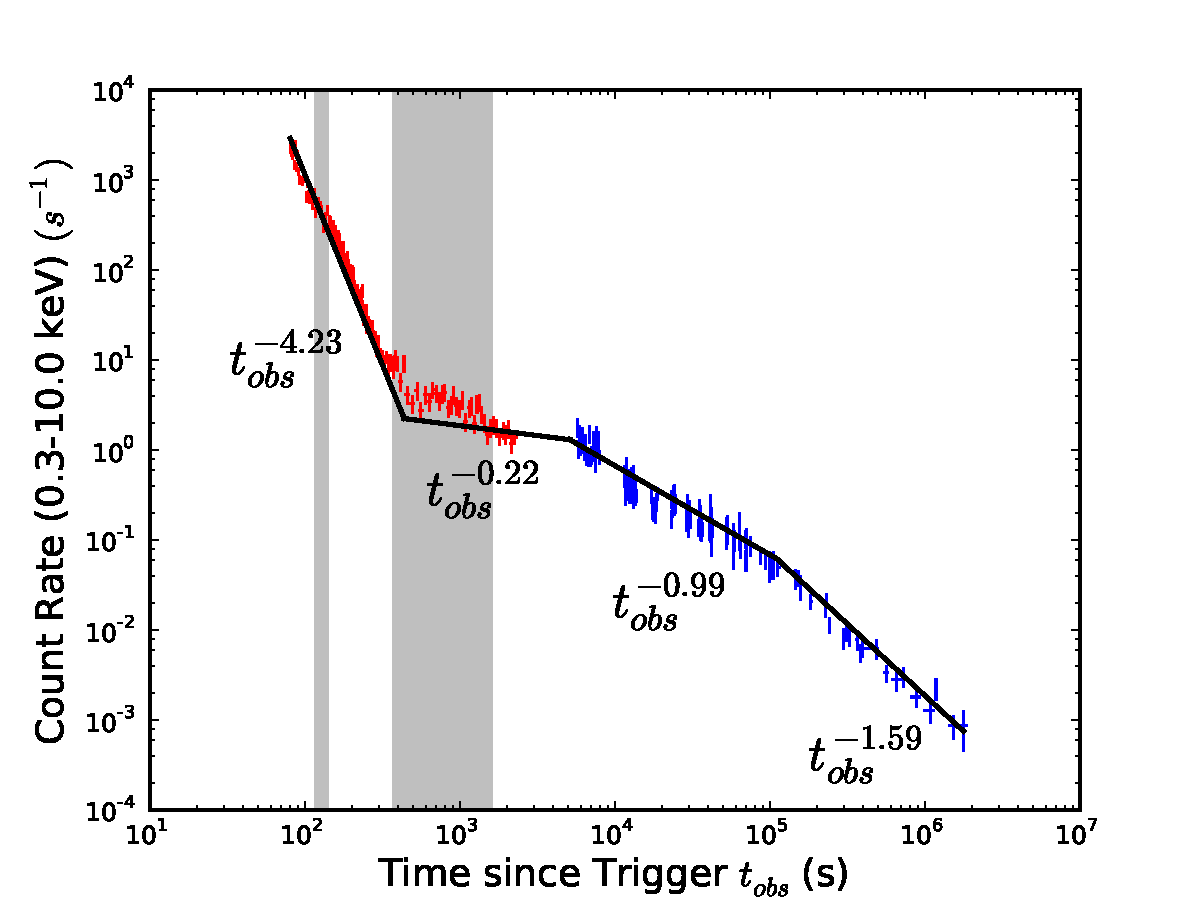
\includegraphics[width=0.8\textwidth]{figures/scalefit/data_trim.pdf}
 \end{center}
	\caption{\figlabel{trim}  The data trimming procedure demonstrated for GRB 100621A.  Blue data are kept for the fit, while red data are removed.  The best-fit power law is obtained from the \swiftXRT{} catalogue.  The last three segments of the power law undergo monotonic decay, but the only the last two are kept because we require the slope must be less than $-1/4$.  Flares (shaded rectangles) are cut out if they occur during the monotonic decay. }
\end{figure}

We use the Counts-to-flux conversion factor calculated calculated separately for each power law segment of the light curve.  In principle this could include data obtained in either Windowed Timing (WT) or Photon Counting (PC) modes of the \swiftXRT{}, but in practice our trimming leaves only PC mode data for the analysis.  The Counts-to-flux conversion factors are calculated from a spectral fit over the entire power-law segment and hence are time-averaged.  Since the spectrum of X-ray afterglows tends not to evolve after the steep decay, these time-averaged values should be sufficient for our analysis. 

It is possible after these cuts some light curves may have an insufficient number of data points to perform a seven-dimensional fit.  Our last requirement on the data is that a light curve have at least 3 degrees of freedom (ie. 11 data points in a 7 parameter fit) to attempt the analysis.  After all cuts were applied 226 light curves had a sufficient number of data points, on average 109 per burst.  These bursts form the sample for our study.

%%%%%
%Section 4 - Analysis
%%%%%


\section{The Analysis}

Our afterglow model has ten parameters, which we refer to collectively as $\Theta$:
\begin{equation}
	\Theta \equiv \left \{  z, d_L, \Eiso, n_0, \thO, \thobs, p, \epse, \epsB, \xN \right \} \ .
\end{equation}
We employ a Markov-Chain Monte Carlo (MCMC) approach to fit each light curve $D$ in our sample to the model.  The MCMC algorithm generates samples of the posterior probability distribution $p(\Theta | D)$, the probability distribution of the parameters $\Theta$ given the light curve data $D$.  This approach gives more information about the global structure of the posterior than a standard $\chi^2$ minimization, providing very accurate information about the uncertainties in the inferred values of any parameter or set of parameters.

Generating light curves from scaling laws can create degeneracies between parameters if the data lies entirely in a single spectral regime (eg. fast cooling with $\nu > \nu_m$).  Additionally, a degeneracy exists between $\epse$, $\epsB$, and $\xN$ \citep{Eichler05}.  The degenerate parameters may vary over several orders of magnitude but will produce identical light curves if certain ratios between the parameters remain fixed.  Degenerate parameters will be left unconstrained in the final analysis.  The uncertainty in these parameters will be incorporated into our estimates for non-degenerate parameters through marginalization: integrating the posterior over these \emph{nuisance parameters}.

The posterior $p(\Theta | D) $ is calculated from the likelihood $p(D | \Theta)$ and the prior $p(\Theta)$ via Bayes' Theorem:
\begin{equation}\eqlabel{bayes}
	p(\Theta | D) \propto p(\Theta) p(D | \Theta) \ .
\end{equation}
The proportionality constant in \eqrefp{bayes} accounts for normalization, and is irrelevant in the MCMC analysis.  Assuming the data points ($t_i,F_i$) are mutually independent with gaussian uncertainties $\sig_i$, we can write the likelihood as a standard $\chi^2$:
\begin{align} \eqlabel{likelihood}
	p(D|\Theta) &\propto \exp\left(-\frac{1}{2} \chi^2 \right) \ ,\nonumber \\
    \chi^2 &= \sum_{i} \left(\frac{F_i - F_{model}(t_i; \Theta)}{\sig_i}\right)^2 \ , 
\end{align}
where $F_{model}(t_i, \Theta)$ is the flux calculated from our model at time $t_i$ with parameters $\Theta$, integrated over the \swiftXRT{} spectral band $0.3 - 10.0$ keV.  The assumption of gaussian uncertainties is valid for sufficiently high photon counts per flux measurement $F_i$.  The UKSSDC \XRT{} light curve bins maintains at least 15 photon counts for each $F_i$, we take this to be sufficient for Gaussian uncertainties \citep{SWIFTauto}.  

The prior $p(\Theta)$ is used to constrain and fix the parameters of the fit using prior knowledge of the data and model.  To reduce the dimension of the fit we fix $z$, $d_L$, and $\xN$.   The redshift $z$ is fixed to the current measured value (see footnote \ref{ft:z}).  The luminosity distance $d_L$ is calculated from $z$ using a benchmark $\Lambda CDM$ cosmology with $H_0 = 71\text{km}\ \text{s}^{-1} \text{Mpc}^{-1}$ and $\Omega_m = 0.27$.  There is a well known degeneracy in our formulation between $\epse$, $\epsB$, and $\xN$, to resolve this we fix $\xN = 1$ for all afterglows.

Some transformations are performed on the free parameters in $\Theta$ to improve performance.  The dimensionfull parameters $\Eiso$ and $n_0$ are made dimensionless via \eqrefp{rescale}, parameters which may vary over several orders of magnitude are put on a log-scale, and $\thobs$ is measured as a fraction of $\thO$ (conforming to the organization of the tables).  These transformed parameters, $\Theta_{fit}$, are directly used in the MCMC routine.
\begin{align}
    \Theta_{fit} \equiv& \left \{  \log_{10} \Edl, \ \log_{10} \ndl, \ \thO, \ \thobs  / \thO, \right . \nonumber \\
    &\qquad \left . p, \ \log_{10} \epse, \ \log_{10} \epsB \right \} \ .
\end{align}
The prior on each of these parameters is uniform within certain bounds given in \tab{bounds}.  The bounds on $\Edl$, $\ndl$, $\epse$, and $\epsB$ were chosen to contain the phenomenologically interesting regions of parameter space while eliminating unphysical regions.  The bounds on $\thO$ reflect that our numerical model is based entirely on the simulations presented in \cite{vanEer12boxfit}, which were only performed for $\thO < 0.5$ rad. The full release of \scalefit{} will include opening angles up to $\pi/2$ rad.  The upper bound $\thobs/\thO<1$ encodes that we must lie within the cone of the jet to observe the prompt emission.  The lower bound on $p$ is mathematically necessary for this parameterization, as $p<2$ would require an additional cut-off parameter on the accelerated particle distribution to prevent the total energy from being divergent \citep[see e.g. discussions in][]{Granot02, vanEer13review}. The upper bound was chosen to be high enough to contain the physically likely values.

In code tests, we found fits were not very sensitive to the overall scale of the light curve.  Raising or lowering all the flux values by 20\% did not induce significant changes in our conclusions.  This is a benefit, as it means our analysis are somewhat insensitive to the exact value of Counts-to-flux used, particularly to the specifics of accounting for galactic and extragalactic hydrogen absorption.
%{\bf  Our tests did not include spectral evolution, which can alter the time dependence of Counts-to-flux.  Observations indicate {\bf X-ray} afterglows do not undergo strong spectral evolution on the time scales we are investigating.}

\begin{table}
\begin{center}
\begin{tabular}{cc}
\hline \hline
Parameter & Prior \\[2pt]
\hline
$z$ & Fixed by catalogue \\[2pt]
$\ddl$ & Fixed by $z$ and cosmology\textsuperscript{a} \\[2pt]
$\log_{10} \Edl$ & $[-10.0,3.0]$  \\[2pt]
$\log_{10} \ndl$ & $[-5.0,5.0]$ \\[2pt]
$\thO $& $[0.045,0.5]$ \\[2pt]
 $\thobs / \thO$ & $[0.0,1.0]$ \\[2pt]
$p$ & $[2.0, 5.0]$ \\[2pt]
 $\log_{10} \epse$ & [-10.0, 0.0] \\[2pt]
$\log_{10} \epsB$ & [-10.0, 0.0] \\[2pt]
$\xN$ & Fixed at $1.0$ \\[2pt]
\hline
\multicolumn{2}{l}{\textsuperscript{a}We use a benchmark $\Lambda$CDM cosmology with $H_0 = 71\text{km}\ \text{s}^{-1} \text{Mpc}^{-1}$ and $\Omega_m = 0.27$.} \\
\multicolumn{2}{l}{Parameters which are not fixed are given a uniform prior within the bounds above.}
\end{tabular}
\end{center}
\caption{Priors for parameters in $\Theta$. \tablabel{bounds}}
\end{table}


The MCMC analysis is performed using the parallel-tempered affine-invariant ensemble sampler implemented by the \emcee{} python package.  This algorithm uses an ensemble of ``walkers'' moving simultaneously through parameter space instead of the standard single walker approach (e.g. Metropolis-Hastings).  The use of the ensemble allows the method to be affine-invariant: affine transformations of the distribution do not affect the efficiency of the sampling.  Strong linear correlations between parameters are sampled with the same quality as uncorrelated parameters, a difficult problem for traditional samplers.  

Parallel tempering is a technique used to better sample multimodal distributions (\citet{Swendsen86, Geyer91}, see \citet{Earl05} for a review).  Several ensembles are run simultaneously on likelihoods $p(D|\Theta)^{1/T}$, where $T$ is the temperature.  The lowest temperature ensemble $T=1$ samples the true posterior, while hotter ensembles sample distributions which more closely resemble the prior and hence are less restricted in their movements.  The ensembles are coupled by allowing walkers to swap between them with some probability every iteration.  This allows walkers to mix between distant modes, allowing efficient sampling of multimodal distributions.  Parallel tempering is tuned by the choice of temperature ladder: the temperature of each ensemble.  We use the default ladder provided with \emcee{}: a geometric sequence of user set length and growth factor tuned to optimally sample an n-dimensional gaussian.  Only samples from the true distribution ($T=1$) are used in the analysis.

For reasonable parameter values in our ISM model both $\nu_m$ and $\nu_c$ lie below the \swiftXRT{} band at late times.  As such, a large number of X-ray light curves generated by \scalefit{} will exist in only a single spectral regime.  In this case the scaling relations used to calculate the flux will create a large degeneracy between $\Eiso$, $n_0$, $\epse$, and $\epsB$, leading to high correlations between these parameters.  Affine-invariance is thus a highly beneficial property of the sampler for this analysis.

Each afterglow was sampled with 20 temperature levels and 100 walkers per level, centered in a small ball around the reference point in phase space:
\begin{equation}\eqlabel{init}
	\Theta_{fit, 0} = \{0.0, \ 0.0,\  0.2, \ 0.5,\  2.5, -1.0, -2.0\} \ .
\end{equation}
Walkers were initialized with uniform random values within 2\% of \eqrefp{init} in each non-zero reference value, and within $\pm 0.02$ if the reference value was zero.  There currently does not exist any unbiased method for determining the convergence of an MCMC chain.  As such we employed a pragmatic view for determining the ``burn-in'' and running lengths of the chain.  Initial tests indicated the autocorrelation time of the chain to be approximately 1000 iterations, depending on the parameter.  Based on this we chose a burn-in of 7000 iterations, to ensure several autocorrelation times between the initial condition and the recording of samples.  Sampling was performed for 3000 iterations after burn-in, generating altogether 300 000 samples of $p(\Theta_{fit} | D)$ for each burst.

For each burst the final values of the fit parameters are inferred from their marginalized posteriors (eg. $p(\thobs |D)$) estimated by the MCMC generated samples.  The marginalization incorporates the uncertainties in all other fit parameters.  Our estimate for each parameter is the median of the posterior, with uncertainty given by the $68\%$ quantiles.  We use the median (instead of the mean or mode for instance) because it is less sensitive to the tails of the distribution and it is preserved under invertible mappings of the parameter (eg. $\log_{10} \epse \to \epse)$.

%chi^2 on approximate gaussianness
	
We validated this analysis by performing fits on a set of synthetic data.  Using the \scalefit{} model we produced a set of 500 light curves with randomly distributed parameters $\Theta$ in the \swiftXRT{} 0.3-10.0 keV band, using the method from \citet{vanEer11}.  Data points were drawn from each light curve in a manner to resemble \swiftXRT{} data.  Occultation by the Earth was taken into account by only taking data in 48 minute intervals, and the fractional exposure of late-time afterglows was included by reducing the data rate by a factor of ten for $t_{obs} > 1$ day.  Fluxes were given random gaussian uncertainties (25\% for early time and 50 \% for late time).  Each of these synthetic light curves was subjected to our analysis using a single ensemble of 1500 walkers and no parallel tempering.    

\begin{figure*}
\begin{center}
    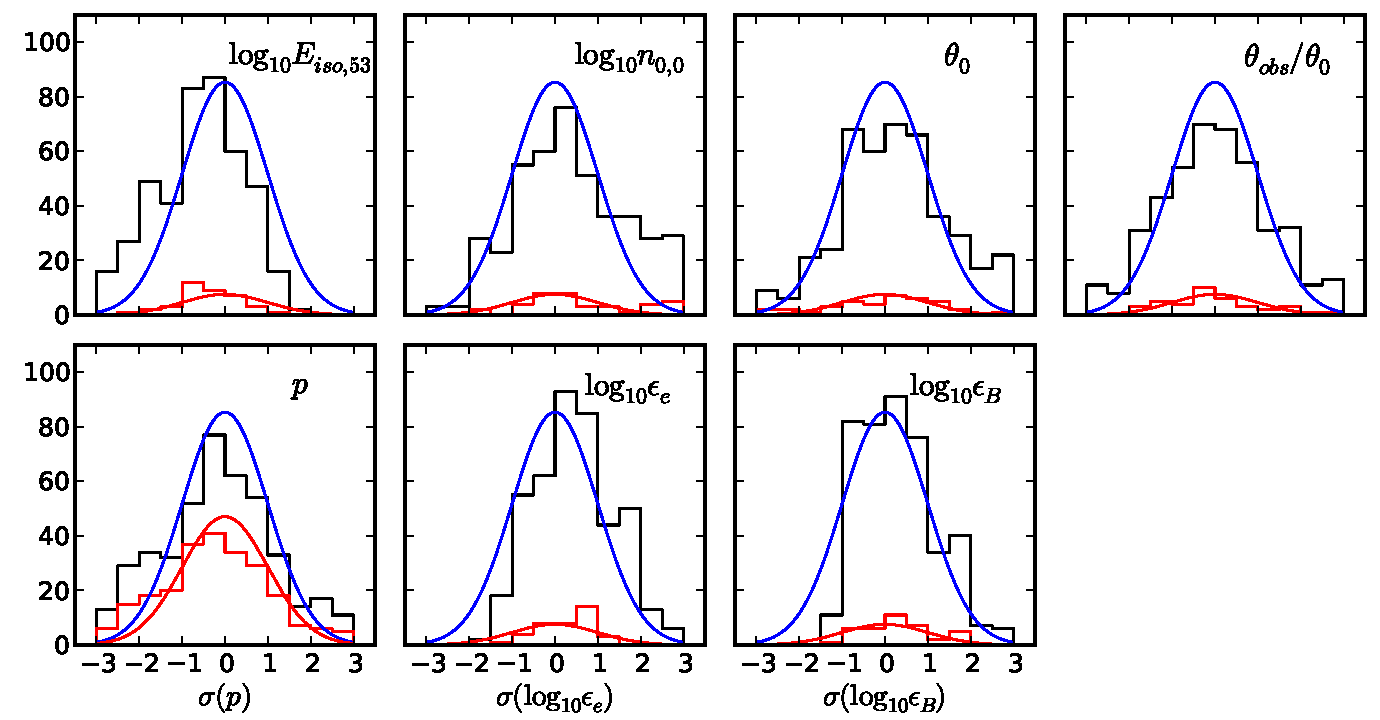
\includegraphics[width=0.8\textwidth]{figures/scalefit/discrepancies.pdf}
\end{center}
	\caption{\figlabel{test} The discrepancy ($\sig$) between true and estimated values of $\Theta_{fit}$ in fits to synthetic data are shown in the black histograms.  A discrepancy $ \sig=\pm 1$ ($\pm 2$) indicates the true value lies on the 68\% (95\%) quantile of the estimate.  The blue curve shows the theoretical distribution of discrepancies: a gaussian normalized to the number of synthetic datasets with unit width.  The red curve and histogram shows the same distributions after cutting to ``well-fit'' curves (our definition of ``well-fit'' is introduced in Section 5).  These results were run with a single ensemble of 1500 walkers, no parallel tempering.}
\end{figure*}

\fig{test} shows the a histogram of discrepancies between the true and estimated values for $\Theta_{fit}$ for each synthetic afterglow.  Theoretically these distributions should be approximately Gaussian.  The tails of the distributions for $\Edl$, $\ndl$, and $\epse$ indicate this analysis may underestimate $\Edl$ and overestimate $\ndl$ and $\epse$.  Due to the degeneracies in these parameters when fitting only a single band, this is not entirely surprising.  The distribution of discrepancies for $\epsB$, $\thO$, $\thobs/\thO$, and $p$ agree with the expected Gaussian shape, indicating the analysis is at least internally consistent on these parameters.  We believe this is sufficient indication that \scalefit{} can provide good estimates of $\thO$, $\thobs / \thO$, $p$, and $\epsB$ when fitting single band X-ray afterglow light curves.  Further runs on the synthetic data demonstrated our results are not altered when fitting the spectral flux $F_\nu$, flux $F$, or fluence $\int F dt$.

In testing it was discovered $p(\Theta_{fit}|D)$ may be strongly multi-modal, particularly when light curves are allowed to extrapolate outside the calculated tables for $\cfp$, $\cfm$, and $\cfp$.  In some cases, the multi-modality is strong enough that parallel tempering cannot adequately sample the distribution.  To minimize the effect of these cases we adopted the following heuristic.  Every light curve is fit twice, once allowing extrapolation (to a maximum of one order of magnitude in $\tau$) and once with no extrapolation.  The results we report are from the run that found the lowest $\chi^2$: the sample with highest likelihood.    

A parallel effort has been performed using the same model theoretical model with an independent implementation \citep{Zhang14}.  This study focuses on a smaller number of bursts which were observed by both the \swiftXRT{} and \chandra{} and uses \multinest{} sampling for its analysis.  Both methods were tested during development for convergence, sensitivity to initial conditions, and behaviour with resolution.  The results were consistent between both analyses, demonstrating the robustness of the methods and providing a measure of independent validation.

%%%%%
%Section 5 - Results
%%%%%

\section{The Results}

We ran the \scalefit{} analysis on all 188 afterglows in our sample.  \tab{results}, located in the Appendix, gives results for the non-degenerate parameters ($\thO, \thobs/\thO, p$).  The quality of the fits varied from burst to burst.  Some bursts had very sharp fits, most had a broad (ie. unconstrained) distribution in at least one of the parameters of interest.  A small minority of fits ($\lesssim10\%$) were unable to converge to an adequate light curve, with a best fit $\chi^2/dof \gg 1$.  Given the freedom in our model, we expect the afterglows in the latter category do not satisfy one or more of our base assumptions, perhaps that of a homogeneous ISM.

The fit for GRB 110422A is shown in \fig{fit1}. It serves as an example of a particularly good fit.  The ``corner plot'' shows projections of $p(\Theta_{fit} | D)$ as determined by the MCMC samples.  Plots on the diagonal show the marginalized distributions for each individual parameter, while the off-diagonal plots show $p(\Theta_{fit} | D)$ marginalized over all but two parameters.  We see the distributions of $\Edl$, $\ndl$, $\epse$, and $\epsB$ are very broad, covering several orders of magnitude.  This of course is due to the model's degeneracy between these parameters, which induces a strong correlation between them. This correlation is exhibited in the off-diagonal plots for these parameters.  The energy and circumburst density ($\Edl$ and $\ndl$) are confined to narrow bands in phase space, while $\epse$ and $\epsB$ exhibit a multidimensional degeneracy.  This degeneracy does not affect the distributions of $\thO$, $\thobs/\thO$, or $p$, as can be seen from their plots on the diagonal.  Despite several other parameters being unconstrained, these parameters are determined quite well.  We find $\thO = 0.0733^{+0.011}_{-0.0098}$ rad, $\thobs/\thO = 0.676^{+0.035}_{-0.050}$, and $p=2.284^{+0.049}_{-0.06}$.  In particular, this afterglow was almost certainly observed off-axis.

\begin{figure*}
\begin{center}
\begin{overpic}[width=\textwidth]{figures/scalefit/110422A_corner.pdf}
	\put(46,60){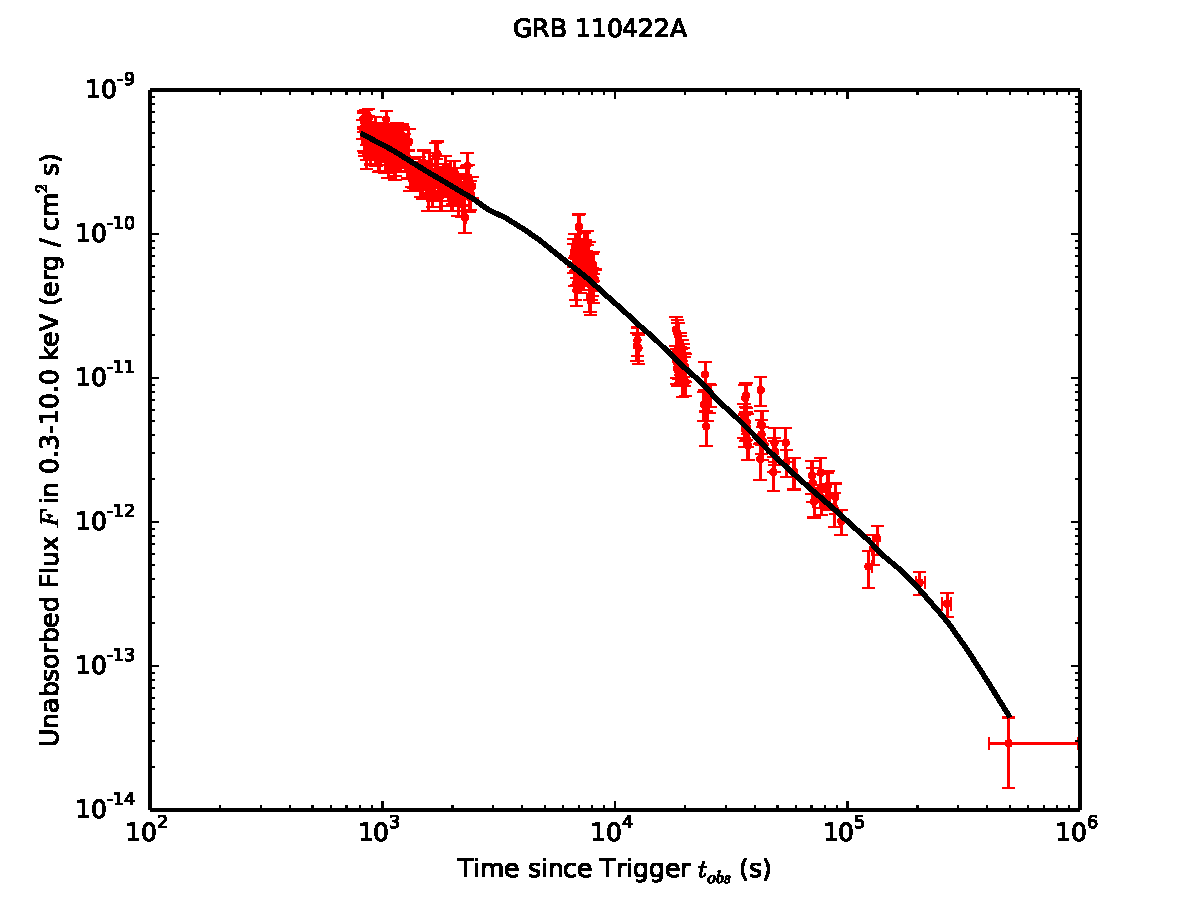
\includegraphics[width=0.55\textwidth]{figures/scalefit/110422A_lightcurve.pdf}}
\end{overpic}
\end{center}
\caption{Fit result for 110422A.  This ``corner plot'' shows all one dimensional (diagonal) and two dimensional (off-diagonal) projections of the posterior pdf.  The best-fit values (MAP, maximum posterior probability) are shown in blue.  Dotted lines mark the 16\%, 50\%, and 84\% quantiles of the marginalized posteriors for each parameter.  The best-fit light curve is shown against the data in the upper right. \figlabel{fit1}}
\end{figure*}

In general, the posterior distributions of $\Eiso$ and $n_0$ tend to be very broad or uniform, with a tight pairwise correlation between them.  The correlation is caused by the rescaling of $t_{obs}$ to $\tau$, which depends on the ratio $\Eiso/n_0$.  The radiation parameters $\epse$ and $\epsB$ tend to demonstrate a more multidimensional degeneracy with $\Eiso$, $n_0$, and each other.  These reflect the inherent degeneracy in our model when restricted to single band fits.  $\epsB$ is least constrained by most fits.  This is not unexpected as the overall dependence of the flux $F$ on $\epsB$ is very weak.  For example, above the cooling break $F_\nu \propto \epsB^{(p-2)/4} \approx \epsB^{0.05}$ using our median value of $p$.  We expect these difficulties to ease in multi-band fits.

On the other hand $\thO$, $\thobs$, and especially $p$ are constrained well by several fits.  This is not surprising, as the dependence of the light curve on these parameters is not given by simple power-law scaling.  With these estimates for $\thO$, $\thobs$, and $p$ we can make some statements about the global distribution of these parameters amongst the \swiftXRT{} sample.  

\begin{figure*}
	\begin{center}
	\begin{tabular}{cc}
    		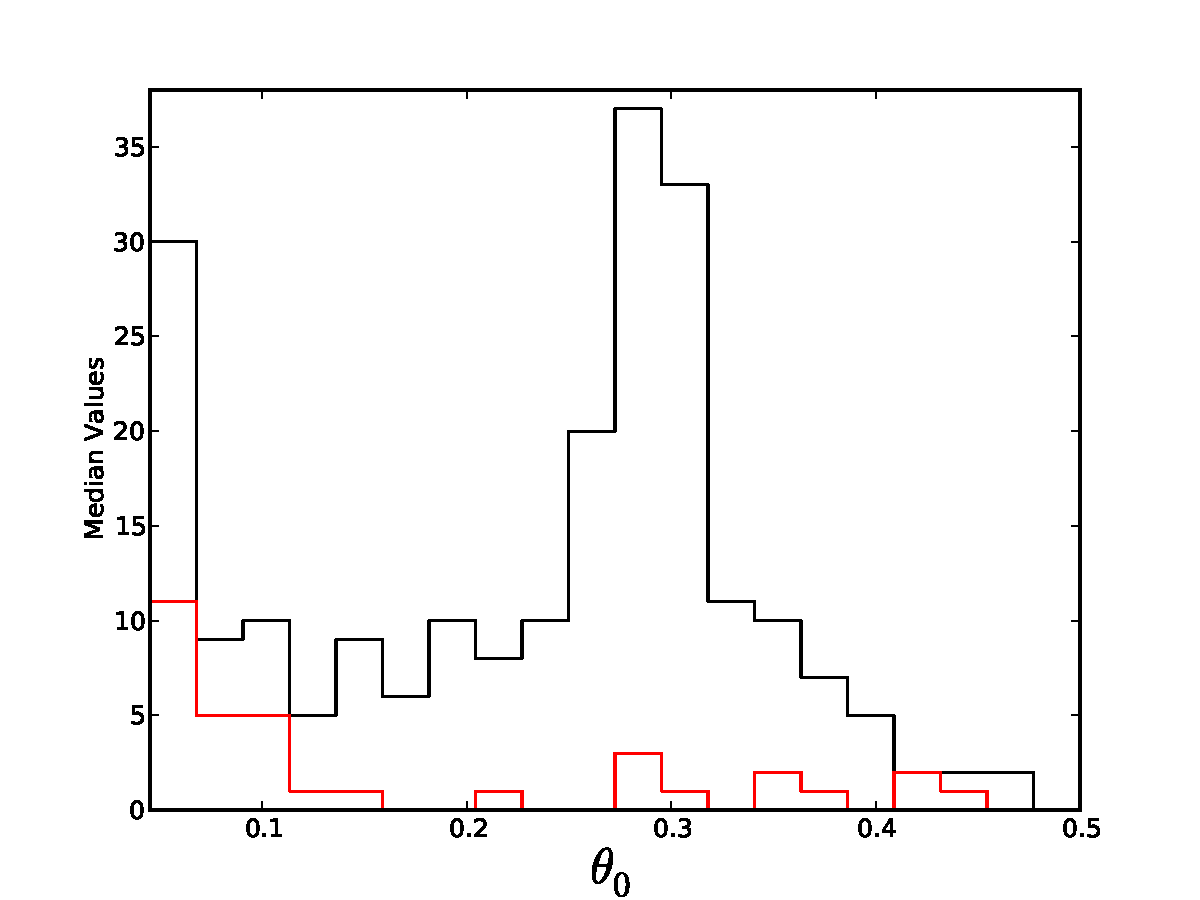
\includegraphics[width=0.45\textwidth]{figures/scalefit/distribution_Th0.pdf} & 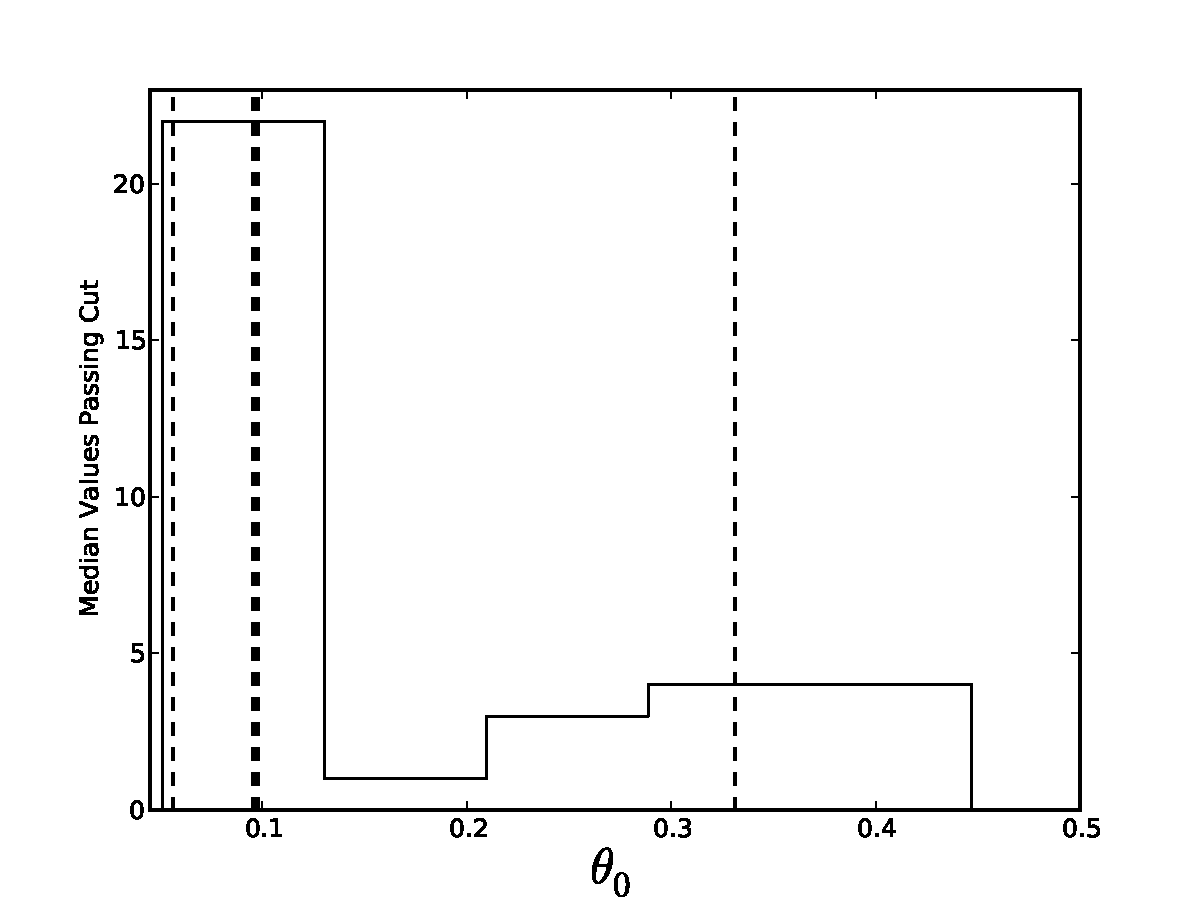
\includegraphics[width=0.45\textwidth]{figures/scalefit/distribution_cut_Th0.pdf}
    	\end{tabular}
    	\end{center}
	\caption{\figlabel{thO} Distribution of $\thO$ across all afterglows in the sample. The black curve in the first figure shows the distribution of reported values of $\thO$ (eg. the median of the marginalized distribution for each light curve).  The red curve plots the same, including only bursts considered ``well-fit'' in $\thO$ and $\thobs$.  The second figure shows only the ``well-fit'' bursts, with the median (thick dashed) and  68\% quantile (thin dashed).}
\end{figure*}

\begin{figure*}
\begin{center}
	\begin{tabular}{cc}
   		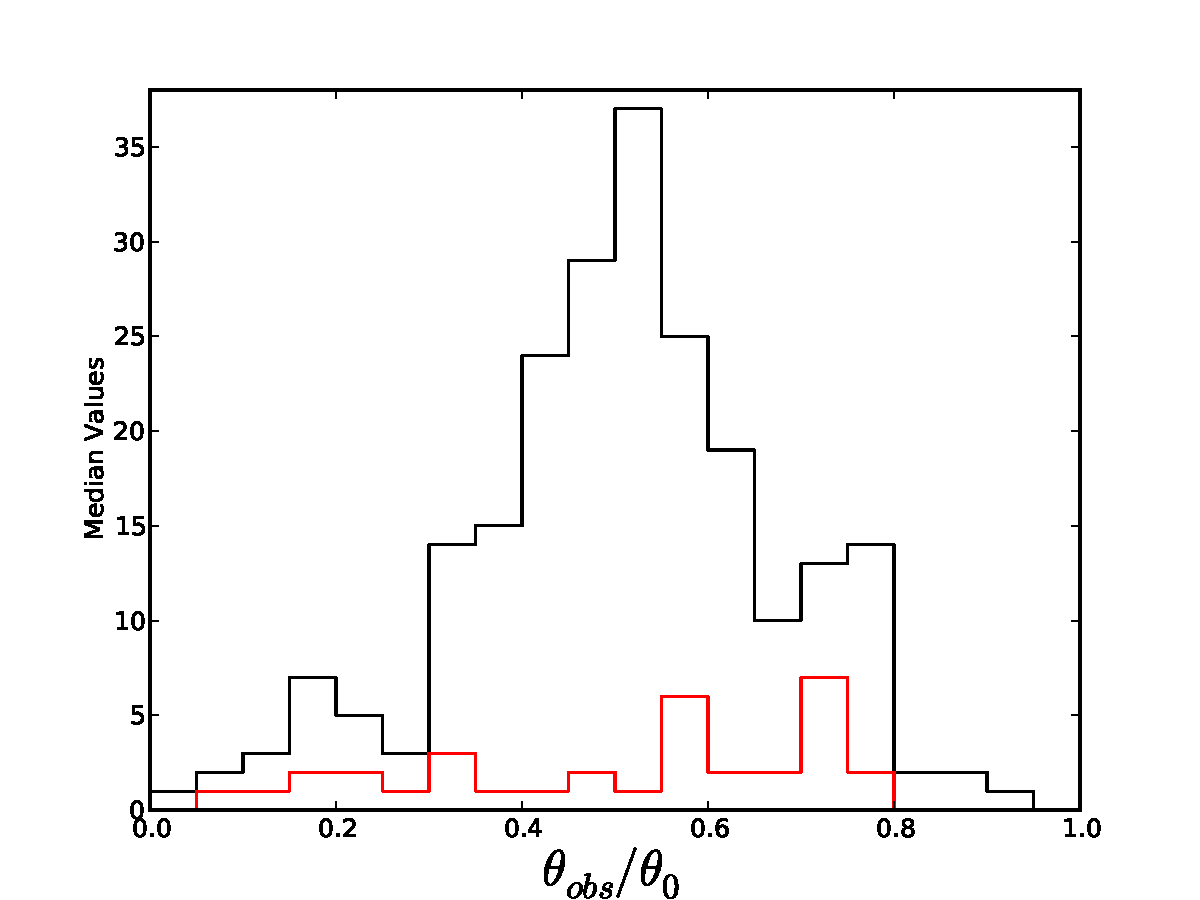
\includegraphics[width=0.45\textwidth]{figures/scalefit/distribution_ThObs.pdf} & 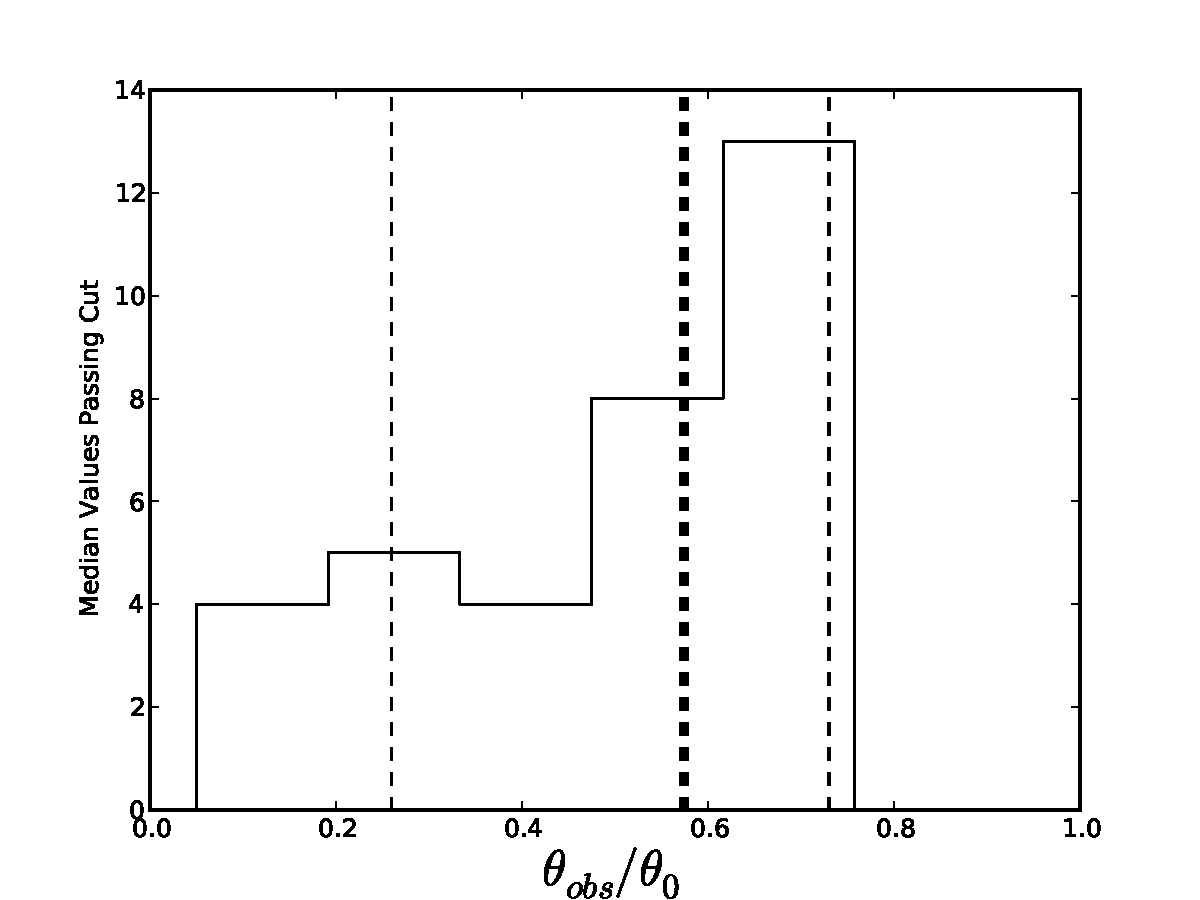
\includegraphics[width=0.45\textwidth]{figures/scalefit/distribution_cut_ThObs.pdf}
    	\end{tabular}
    	\end{center}
	\caption{\figlabel{thobs} Same as \fig{thO}, but for $\thobs / \thO$.}
\end{figure*}

\begin{figure*}
	\begin{center}
	\begin{tabular}{cc}
    		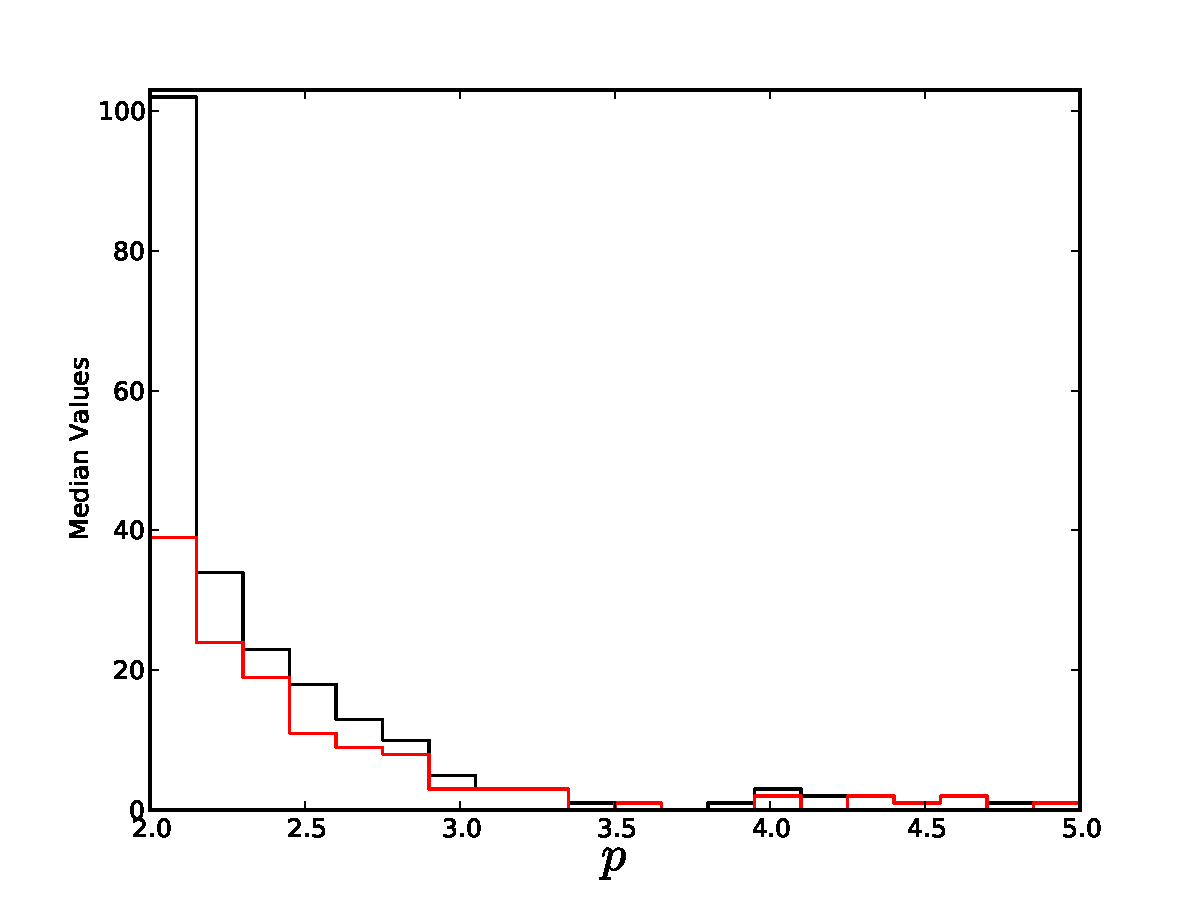
\includegraphics[width=0.45\textwidth]{figures/scalefit/distribution_p.pdf} & 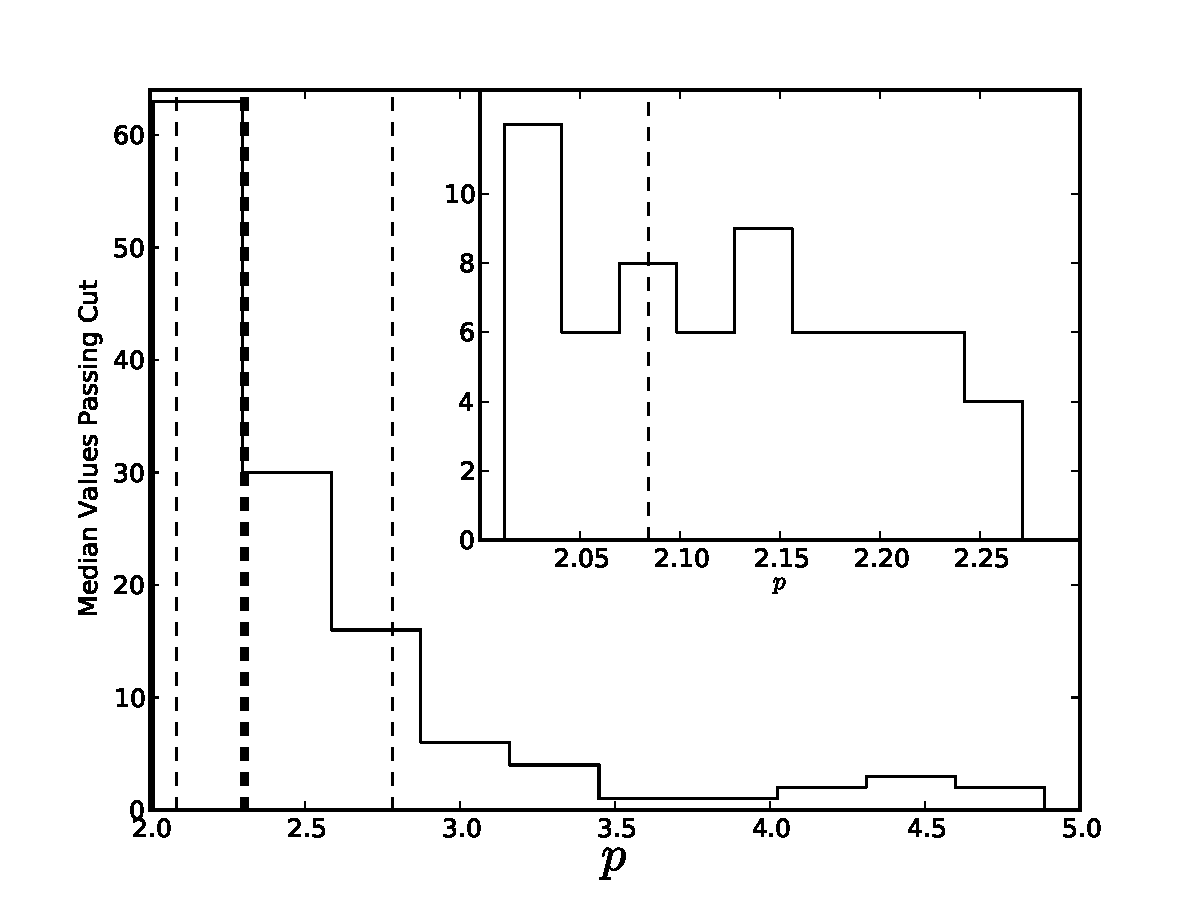
\includegraphics[width=0.45\textwidth]{figures/scalefit/distribution_cut_p.pdf}
    	\end{tabular}
    	\end{center}
	\caption{\figlabel{p} Same as \fig{thO}, but for $p$.  The ``well-fit'' criteria is applied only to $p$ and the inset is zoomed to $2.0 < p < 2.3$.}
\end{figure*}

In first panels of Figures \figref{thO}, \figref{thobs}, and \figref{p} we plot histograms of the estimated values for $\thO$, $\thobs/\thO$, and $p$ for our sample.  The opening angle $\thO$ has a broad distribution with isolated peaks at $\thO \sim 0.05, 0.28$ rad.  The observer angle $\thobs / \thO$ is broad, with a spike at $\thobs/\thO \sim 0.5$. The spectral index $p$ decreases from $p\sim 2.1$ into a tail which extends to $p=3$.  Since these plots include fits which had unconstrained distributions, they do not reflect the true distributions $P(\thO)$, $P(\thobs)$, $P(p)$ in our sample.  For instance, the large spikes near the domain center in Figures \figref{thO} and \figref{thobs} are due to including the medians of distributions which were almost uniform.   

To resolve this we make cuts on our dataset to eliminate poorly-constrained fits.  We employ the following criterion to qualify a particular parameter as ``well-fit'': the width of the 68\% quantile must be less than half the width of parameter's domain (see \tab{bounds}) and the best-fit (maximum posterior, minimum $\chi^2$) value must lie within the 68\% quantile.  The number of light curves passing each criterion are given in \tab{passed}.

\begin{table}
\begin{center}
\begin{tabular}{cc}
\hline \hline
Parameter & Number of Well Fit Light Curves \\
\hline
$\thO$ & $53$  \\
$\thobs / \thO$ & $63$ \\
$p $& $128$ \\
 $\thO$ and $\thobs / \thO$ & $ 34$ \\
$\thO$,  $\thobs / \thO$ and $p$ & $15$ \\
\hline
\end{tabular}
\caption{Number of light curves passing the ``well-fit'' criteria for each parameter. \tablabel{passed} }
\end{center}
\end{table}

For a burst to be considered ``well-fit'' and included in the global distribution of $\thO$ and $\thobs$ we require it to have passed the criteria for both $\thO$ and $\thobs$.  There are 31 such light curves in our sample, the histograms of their values of $\thO$ and $\thobs / \thO$ are given in the second panels of Figures \figref{thO} and \figref{thobs} respectively.  For a burst to be included in the global distribution of $p$ we only require it to be ``well-fit'' in $p$.  There are 108 of these bursts, the histogram of their values of $p$ is given in the second panel of \fig{p}.  Summary statistics of these histograms are given in tab{quantiles}.

\begin{table}
\begin{center}
\begin{tabular}{cccc}
\hline \hline
Parameter & Median & 68\% Quantile & 95\% Quantile \\ [0.5ex]
\hline
$\thO$ &  $0.097$ & $(0.056, 0.33)$ & $(0.055, 0.42)$\\
$\thobs / \thO$ & $0.57$ & $(0.26, 0.73)$ & $(0.16, 0.75)$ \\
$p $& $2.30$ & $(2.08, 2.78)$ & $(2.03, 4.05)$ \\
\hline
\end{tabular}
\end{center}
\caption{Quantiles on distribution of fit values for $\thO$, $\thobs / \thO$, and $p$. \tablabel{quantiles}}
\end{table}


\underline{Half opening angle $\thO$}: We find half of the well-fit bursts have a small opening angle $0.045 < \thO < 0.097$ rad.  The remainder are broadly distributed throughout the allowed range $0.097 < \thO < 0.5$ rad.  As the lower cutoff at 0.045 rad is a reflection of our simulation coverage and prior, it is possible some of the small angle bursts in fact have $\thO < 0.045$ rad.  Our results are consistent with \cite{Racusin09}, who found a similar distribution of $\thO$ with a median of 0.094 rad.

\underline{Off-axis observer angle $\thobs$}:  The $\thobs  / \thO$ distribution is broad with a median at 0.57 and 95\% quantiles at (0.16, 0.75).  These afterglows are almost certainly observed off-axis, at a significant fraction of the opening angle.  This can have a profound effect on afterglow light curve analysis.  Jet-breaks occur when the emission surface seen by an observer begins extending beyond the edges of a jet, causing the light curve to sharply steepen.  When viewed off-axis the near edge of the jet will be seen before the far edge, causing the jet-break transition to become extended over time  \citep{vanEer12obs, vanEer13boost}.  It may be very difficult to see off-axis jet breaks without late-time observations.

\underline{Electron spectral index $p$}:  More than half of our entire sample passed the well-fit criteria for $p$.  The distribution of fit values for $p$ spans the allowed domain, favouring smaller values $p < 2.30$.  Some concern may be raised that so many bursts seem to require values so close to the $p>2$ boundary imposed by the prior.  From inspection of individual fits, we find this is not the case.  Bursts with well-fit $p$ distributions centered near 2 tend to be very sharply peaked, so that the $p=2$ case is safely in the tails (eg. \fig{fit1}).  Similarly, we find no indication of interference from the $p<5$ upper bound.  

\subsection{Short Bursts}

Nine short GRBs were included in our sample\footnote{The short GRBs 050509B, 070429B, and 100206A did not have enough data points to be included.}.  Unfortunately few of them produced useful results from our analysis.  GRBs 060801, 070724A, 070809, 080905A, 100117A, and 101219A were unable to find a good fit: all had very broad distributions and a minimum $\chi^2/dof  > 2.0$.  GRBs 090426 and 100724A found reasonable fits, but still do not have enough data to constrain the parameters.  These bad fits could be the result of being over-aggressive in our data selection, inappropriate priors, or that these afterglows break one or more of our model assumptions.  

On the other hand, GRB 051221A produced a good fit with $\thO = 0.448^{+0.031}_{-0.038}$ rad, $\thobs/\thO = 0.449^{+0.053}_{-0.058}$, and $p = 2.024^{+0.025}_{-0.014}$.  This indicates the afterglow was most likely caused by a very broad jet, and was observed significantly off-axis.  The $p$ value is quite small, with the distribution running directly into the lower bound at $p = 2.0$.  This indicates a need for followup with a model that can provide for $p < 2$.

\citet{Zhang14} find a different best-fit: $\thO = 0.10$ rad, $\thobs/\thO = 0.08$, and $p=2.36$.  Their results are consistent with ours, however, as their posterior distributions are quite broad and have significant weight in our reported region.  Our fit uses only \swiftXRT{} data and begins at $t_{obs} = 1877$ s, while their fit includes late time \chandra{} data and only begins at $t_{obs} = 30,864$ s.  To determine the exact source of the difference we did runs with both starting times, both with and without the \chandra{} data.  The \chandra{} data does not strongly affect the fit, rather it is the choice of initial time which strongly determines the result.  

The light curve for 051221A has a plateau from $\sim$2000 s to $\sim$20,000 s which we include as part of the early time segment as it passes the protocol outlined in Section 3.  A detailed analysis of this burst using radio, optical, and X-ray data was given in \citet{Soderberg06}, reporting $0.10 \leq \thO \leq 0.13$ rad, $p = 2.15 \pm 0.10$, $\thobs=0$ (implicitly) and attributing the plateau to an energy injection phase.  Our best-fit, ignoring self-absorption, matches both the radio and X-ray data but systemically under predicts the optical data by a factor of a few.  This discrepancy with the optical could be due to the global cooling time approximation \citep{vanEer10offaxis, Guidorzi14}.  A strong caveat on our fit result is the assumption the plateau is due solely to the observational effects of a decelerating blast wave.  In particular it is difficult to reconcile the regular pre-plateau stage with a pure blast wave model.  If the plateau is indeed due to energy injection, then the \scalefit{} model is inapplicable to the early-time light curve and a later time to begin fitting would be more appropriate.  

Constraining the orientation, $\thobs$, and opening angle $\thO$, of short GRBs remains of specific interest because of the implication for gravitational wave science. If short GRBs are detectable electro-magnetic counterparts to gravitational wave events, constraining their orientation would greatly reduce the degeneracy in the possible fits to the GW signal \citep{Nissanke13, Arun14}.  Additionally, constraining their opening angle will constrain their beaming corrected rates and total energies.

%%%%%%
% Discussion %
%%%%%%


\section{Discussion}

Given the usual cosmological assumptions of isotropy and homogeneity, it is expected that the orientation of GRB jets is random.  Since larger off-axis angles $\thobs$ correspond to a larger solid angle of possible viewing, the theoretical distribution of $\thobs/\thO$ for a homogeneously emitting conical outflow is linear:
\begin{equation}
	P_{theo}(\thobs/\thO) \propto \thobs / \thO \ . \eqlabel{theo}
\end{equation}
However, this is almost certainly not the correct distribution of \emph{observed} $\thobs/\thO$.  The likelihood of observing an afterglow with a particular $\thobs/\thO$ depends not only on the orientation of jets relative to Earth (\eq{theo}), but also on the spreading of the blast wave, the brightness profile across the blast wave, and observational detection biases \citep[see e.g.][]{vanEer12obs}.  The brightness profile of a blast wave has two sources: the structure of the outflow itself and the observational limb-brightening effect.  The structure of outflows arising from GRBs is still unknown.  Many models exist in the literature, including the basic unstructured top-hat and more complicated structured models such as two-component \citep[e.g.][]{Berger03}, power-law decay \citep{Rossi02}, or the boosted fireball \citep{Duffell13B}.  Regardless of the outflow structure, the simple optics of observing a relativistic outflow also produce a limb-brightening effect, enhancing observed radiation from the on-edge region of a blast wave \citep{Meszaros06}.  Both these effects will be rolled into the observed distribution of $\thobs/\thO$, as well as any observational biases which may be present for the particular experiment under consideration.  In principle, given enough data it may be possible to study the structure of the outflow from the observed distribution of $\thobs/\thO$.

Our distribution of $\thobs/\thO$, shown in \fig{thobs}, indicates many afterglows have significant observer angles and very few have $\thobs < 0.2\ \thO$ or $\thobs > 0.8\ \thO$.  Although we are not currently able to make claims to the source of these features, be they due to orientation, structure, or observational biases, the sheer presence of large observer angles in several bursts is of crucial importance to estimates for total jet energy $E_{jet}$.  

Figures \figref{thO} and \figref{thobs} indicate a typical observer angle is $\thobs \approx 0.05$ rad $\approx 3$ degrees.  It is important to state that while these angles are small, they are not insignificant.  Even small off-axis observer angles can have a large effect on the light curve if the opening angle was also small.  In particular, when $\thobs$ is a significant fraction of $\thO$, the jet break is smeared from a sharp feature to an extended transition from pre- to post-break slopes.  The delay in the onset of the post-break slope can be large enough to push the jet break out of \swift{}'s typical viewing window (i.e. 10 days) \citep{vanEer10offaxis, vanEer11}.  Additionally, the smooth transition may hinder efforts to detect jet breaks by broken power-law fits.  Both these effects likely contribute to the  ``missing jet break'' problem.
  
Our results are generally consistent with the complementary study investigating afterglows with observations by both the \swiftXRT{} and \chandra{} \citep{Zhang14}.  This study used the same theoretical model, but with an independent implementation and \multinest{} sampling.  The overall consistency of the results shared by both studies validates the robustness of the model and analyses.  Some individual fits display differences, most of which are due to different choices in selecting how much of the \swiftXRT{} data to attempt to fit.  The inclusion of \chandra{} points can also have a strong effect on the light curve, indicating the utility of using late time followup when it is available.

Possible methods for improving the fit results are currently being studied.  Further work will include the incorporating multi-band data and and a stellar wind circumburst medium into the fits.  Multi-band data should break the degeneracy between $\Eiso$, $n_0$, and $\epse$, allowing much more information to be extracted from the analysis.  Inclusion of stellar wind environments will hopefully lead to more well-fit bursts in this sample.

The full results of this analysis, the posterior probability distribution function (pdf) $p(\Theta | D)$ of each burst in the sample, will be made available online at the Afterglow Library\footnote{\afterglowlibrary}. Researchers interested in using results of this paper are highly recommended to use these instead of the summary statistics presented in the appendix of this paper.  The full 7-dimensional pdf, for instance, may be marginalized to produce a pdf for any subset of $\Theta$, taking into account all correlations between parameters.  The posterior $p(\Theta | D)$ will be made available as a list of MCMC samples in the HDF5 data format.


%%%%%%
% Summary %
%%%%%%

\section{Summary}

We have run the \scalefit{} analysis on a sample of GRB afterglow light curves observed by the \swiftXRT{} between 2005 and 2012.  The sample included all afterglows with a known redshift and a sufficient number of binned light curve points to perform the analysis; 226 light curves in total.  The \scalefit{} afterglow model uses scaling relations in the hydrodynamic and radiation equations to calculate a light curve from precomputed 2d simulations.  Although the model displayed significant degeneracies between $\Eiso$, $n_0$, $\epse$ and $\epsB$, the values of the opening angle $\thO$, observer angle $\thobs$, and spectral index $p$ could be constrained in many bursts.  The \scalefit{} package will be released to the public in the near future \citep[][in prep]{vanEer14scalefit}.

Of the 226 fits, 128 had sufficiently constrained values of $p$ to be included in the result.  We found $p$ has a highly asymmetric distribution, with a median of 2.30 and 68\% quantile $( 2.08 , 2.78)$.  Thirty four bursts in our sample were sufficiently constrained in both $\thO$ and $\thobs / \thO$ to be included in the result.  The distribution of $\thO$ was also highly asymmetric, with a median of $0.097$ rad and a 68\% quantile $(0.056, 0.33)$ rad.  The off-axis observer angle $\thobs/\thO$ had a median of $0.57$ with a 68\% quantile of $(0.26, 0.73)$.  Only four afterglows in the well-fit sample, and thirteen in the full sample, had an observer angle less than $0.2 \thO$.  Therefore, we find that most GRB afterglows are observed off-axis, at a significant fraction of the jet opening angle.  Off-axis viewing can have profound effects on the expected behaviour of the afterglow light curve, delaying and smoothing jet breaks out of the typical \swift{} observing window, which may contribute to the ``missing jet-break problem''.

Our sample include a number of short bursts. Although an orientation was obtained for GRB 051221A, the atypical nature of the light curve decay (including a  possible episode of energy injection, or multi-component jet), renders the application of our decelerating blast wave model questionable in this individual case. Constraining the orientation of short GRBs remains highly desirable given their potential as observable GW counterparts.  The other bursts for which opening angle and orientation are constrained do not share atypical features in the data preceding the regular decay stage.

The full results for this analysis, including the MCMC samples, will be made available on the Afterglow Library.

%%%%%%
% Acknowledgements %
%%%%%%

\section{Acknowledgements}

This research was supported in part by NASA through grant NNX10AF62G issued through the Astrophysics Theory Program, by the NSF through grant AST-1009863, by the Chandra grant TM3-14005X, and by Fermi grant NNX13AO93G.  HvE acknowledges support by the Alexander von Humboldt foundation.  BZ acknowledges the support of SAO contract SV4-74018, NASA contract NAS5-00136, and by SAO grants AR3-14005X, GO1-12102X, and GO3-14067X.  Resources supporting this work were provided by the NASA High-End Computing (HEC) Program through the NASA Advanced Supercomputing (NAS) Division at Ames Research Center. The software used in this work was in part developed by the DOE-supported ASCI/Alliance Center for Astrophysical Thermonuclear Flashes at the University of Chicago.  This work made use of data supplied by the UK Swift Science Data Centre at the University of Leicester.  We thank Judith Racusin, David N. Burrows, Jochen Greiner, David Hogg, and Daniel Foreman-Mackey for their many helpful discussions and comments.

%\section{Appendix - Result Table}

%\begin{table}
%\begin{center}
%\begin{tabular}{ccc}
%a & b & c
%\end{tabular}
%\end{center}
%\caption{All the results \tablabel{results}}
%\end{table}
%

\renewcommand{\chapid}{future}

% Chapter specific commands:

% Math:

\chapter{Future Directions \chaplabel{future}}

Here we briefly summarize future directions for the work presented in this thesis.

\section{Numerical Methods}

The \disco\ shearing mesh is of great advantage when fluid motion is dominantly in the azimuthal direction.  This is completely satisfied by a Keplerian disk above the ISCO.  However, for relativistic problems the region below the ISCO where fluid plunges and the poles where there may be an outflow or jet are often of interest.  For these more complicated problems, the advantage of the moving mesh as it stands is tempered.

A straightforward resolution to this problem is to allow the mesh to move in more than one dimension.  To keep the technical advantages of \disco, the mesh motion cannot be arbitrary.  We desire cell faces to always be coordinate surfaces, determining neighbours to be simple (take linear time), and to not be required to add cells on-the-fly.  The most general scheme which fits these constraints is one where the discretization is such that (taking the \disco\ $r\phi z$ grid as an example):
\begin{enumerate}
	\item Space is foliated by $N_z$ surfaces of constant $z$.  Cells will live in sheets in between these surfaces.
	\item Each sheet is foliated by $N_r(z)$ surfaces of constant $r$, dividing the sheet up into concentric annuli.
	\item Each annulus is divided by $N_\phi(r,z)$ surfaces of constant $\phi$, defining the boundaries of individual cells.
\end{enumerate}
Mesh motion here can be accomplished by allowing each $\phi$, $r$, and $z$ surface to move independently.  When a surface of constant $r$ moves the \emph{entire} annulus moves, as all cells in the annulus share the same $r$ surface.  When a surface of constant $z$ moves the entire sheet moves as a unit, as all cells in the sheet share the same $z$ surface.

This scheme does not require cylindrical coordinates, in fact it can be written in arbitrary coordinates $(x^1, x^2, x^3)$.  If such a scheme were used in an accretion disk simulation, entire annuli could free fall through the ISCO or get lifted in jets.  If the disk heats and expands vertically the mesh could breathe with it.  At the very least this scheme may offer significant time step advantages for 3D disk simulations, where the timestep is dominated by the near light-like velocities of gas at the event horizon.

The energy variable $\tau_U$ has been of great benefit in \grdisco.  Under a similar operation, one could use different spatial basis vectors to calculate the conserved momentum and/or magnetic fields.  Such a scheme could, perhaps, be used to circumvent the notorious problems of the coordinate singularity at $r=0$ by expressing $T^0_i$ and $B^i$ in a basis which is Cartesian (and hence well-defined) near the pole but cylindrical (and angular momentum conserving) away from it.

\section{Black Hole Accretion Disks}

The Kerr parameter of black holes in x-ray binaries is typically measured through continuum fitting to a Novikov--Thorne model or by the iron $K\al$ line.  The excess shock dissipation seen in minidisks could very well be present in x-ray binaries and may bias spin measurements upwards.  A detailed study of the strength of this effect is warranted.

Kilonova are the most likely electromagnetic counterpart to a LIGO source to be observed in the near future. Many key observational characteristics of their emission are still uncertain, particularly how bright the emission from disk winds are.  A good calculation in 3D GRMHD with a physical equation of state and neutrino cooling could greatly elucidate the question.

Tidal excitation of spiral waves, a detailed analysis.  What determines the wave strength? How does it depend on Mach number? Dependence on disk profile, cooling prescription.  Can this be an effect for \emph{realistic} disks?

\section{Binary Black Hole Accretion}

A global characterization of BBH accretion, at least when the circumbinary disk and BH orbital plane are aligned.  A more semi-analytic project, this would use the latest simulation results to inform a model of steady circumbinary accretion. Characterize accretion rate and angular momentum transport rate by fiducial system lifetimes and determine under what conditions disks are thin, slim, or super-Eddington.

Using approximate BBH metric, calculate gas flow in final orbits before merger. Examine to what extent gas gets decoupled from BH evolution, characterize nearby gas right before merger.  

Disk response to BH recoil: using final state of merger runs, replace binary BH with recoiling single and examine disk response.  Prompt emission and shocks?  Under what circumstances?   

In general there is no reason to expect a circumbinary disk to be aligned with the black hole orbital plane.  Examine what can happen if gas and BHs are misaligned.  How strong is the alignment torque? What do minidisks align with?



% Conclusion
\chapter*{Conclusion}\addcontentsline{toc}{chapter}{Conclusion}

In this thesis we have presented a series of works aimed to better understand black hole accretion through numerical simulation.  In \chap{scalefit} we analyzed GRB afterglow light curves with \scalefit, producing the first evidence that GRBs are viewed off-axis.  \chap{numerics} introduced GR-DISCO, a novel moving mesh GRMHD code for simulating disk-like flows.  In \chap{minidisk} we use GR-DISCO to study minidisks in accreting binary systems and identify spiral shock waves as a potentially efficient accretion mechanism.

GRBs are produced by ultra relativistic jets of plasma directed towards Earth.  Although much is unknown about the central engine, the GRB afterglow is a relatively well understood interaction between the ultrarelativistic jet and the circumburst medium.  In \chap{scalefit} we analyze 226 afterglow x-ray light curves from the \swiftXRT, about a third of all recorded GRBs from 2005 to 2012.  Our analysis uses high resolution numerical relativistic hydrodynamic simulations to simulate a blast wave propagating in the circumburst medium.  These simulations are fed into a radiative transfer code to calculate a template bank of high fidelity light curves and spectra.  The \scalefit\ package, developed for this work, performs Bayesian parameter estimation on afterglow light curves by fitting them to this template bank.  The jet opening angle $\thO$, the electron spectral index $p$, and for the first time the observer viewing angle $\thobs$ could be constrained in many bursts.  The distribution of $\thO$ is highly asymmetric with a median of 0.097 rad. The electron index $p$ has a median value of $2.3$ over the sample, consistent with previous results.  The distribution of $\thobs$ has a median of $0.57 \thO$ and only thirteen bursts in the entire sample reported $\thobs < 0.2 \thO$.  This provides the first evidence that GRBs are viewed off-axis, lowering inferred total jet energies by up to a factor of four.  This directly impacts the required power of the central engine, thought to be an accreting black hole or rapidly spinning magnetar.

To further the numerical study of black hole accretion we developed a new GRMHD extension to the moving-mesh code DISCO.  This three dimensional code solves the equations of general relativistic magnetohydrodynamics using sophisticated RIemann solvers and a novel constrained transport algorithm.  The moving mesh allows the code to take longer time steps while reducing error due to numerical diffusion.  In \chap{numerics} we demonstrate the efficacy of GR-DISCO on a number of test problems from relativistic hydrodynamics and relevant to accretion disks.  GR-DISCO is open source and freely available online.

The first use of GR-DISCO is a study of minidisks in binary black hole systems, presented in \chap{minidisks}.  The aim of this work was to better understand the dynamics and observational characteristics of minidisks so as to better inform global simulations of circumbinary accretion and searches for supermassive binary black hole systems.  We find that spiral shocks, excited in the outer minidisk by tidal forces, can propagate to the minidisk interior and efficiently drive accretion.  This allows minidisks to accrete with an effective $\alpha$-parameter $\sim 10^{-2}$ without the need for magnetic fields or other accretion mechanisms.  By ray-tracing through the black hole spacetime we are able to create a synthetic spectrum directly from the radiative losses of the accretion disk.  We find minidisks have a spectrum resembling the standard thin-disk models but with a small high energy excess due to shock dissipation near the innermost stable circular orbit.  Due to scale invariance of the calculation these results can be applied to any accretion disk in subject to tidal forces, in particular x-ray binaries.  

%The development and applications of the methods presented here are ongoing.  The ultimate goal for GR-DISCO is the production of high fidelity, long term simulations of black hole accretion disks.  These simulations, processed through a radiative transfer calculation, could generate a template bank of light curves and spectra.  This would serve as the backbone of a tool like \scalefit, able to constrain the physical parameters of observed accretion disks from a first principles calculation.

This dissertation comprises several works aimed to better understand black hole accretion in a variety of contexts.  \chap{numerics} is primarily methodological, developing a new numerical tool to simulate relativistic accretion disks.  \chap{minidisk} is a detailed a numerical study of a particular system, the minidisks which form during binary black hole accretion.  This study demonstrates the efficacy of spiral shock waves in driving accretion, an effect relevant for both minidisks and x-ray binaries.  \chap{scalefit} uses numerical simulations to develop a model useful to data analysis, providing the first constraints of the gamma-ray burst viewing angle.  Presented here, these works provide a small step towards a better unified understanding of black hole accretion.




% %%%%% Appendices start %%%%%%%%%%%%%%%%
% %% Comment out the following line if your thesis has no appendix
 \appendix
 \chapter{Scalefit Results \label{chap:results}}

%\begin{table}
%\begin{center}
\begin{longtable}{cccccc}
\caption{Median Values of Non-Degenerate Parameters For All Bursts \label{scalefit:tab:results}} \\

\hline \hline
GRB & $\thO$ & $\thobs/\thO$ & $p$ & Min $\chi^2/\text{dof}$ & Extrapolation \\
\hline
\endfirsthead

\hline \hline
GRB & $\thO$ & $\thobs/\thO$ & $p$ & Min $\chi^2/\text{dof}$ & Extrapolation \\
\hline
\endhead

\hline
\multicolumn{6}{l}{\textsuperscript{a} Well-Fit in $\thO$ and $\thobs/\thO$.} \\
\multicolumn{6}{l}{\textsuperscript{b} Well-Fit in $p$.} \\
\multicolumn{6}{p\textwidth}{The median values of the posterior distributions for each of $\thO$, $\thobs/\thO$, and $p$.  Uncertainties are given at the $68\%$ level. The last column denotes whether the fit reported extrapolated in time outside the tabulated values of $\cfp$, $\cfm$, and $\cfc$.} \\
\endfoot

\hline
\multicolumn{6}{l}{\textsuperscript{a} Well-Fit in $\thO$ and $\thobs/\thO$.} \\
\multicolumn{6}{l}{\textsuperscript{b} Well-Fit in $p$.} \\
\multicolumn{6}{p\textwidth}{The median values of the posterior distributions for each of $\thO$, $\thobs/\thO$, and $p$.  Uncertainties are given at the $68\%$ level. The last column denotes whether the fit reported extrapolated in time outside the tabulated values of $\cfp$, $\cfm$, and $\cfc$.} \\
\endlastfoot

050126 & $0.365^{+0.095}_{-0.125}$ & $0.45^{+0.49}_{-0.31}$ & $2.26^{+0.10}_{-0.10}$ & $22.7/4$ & NoEx\\[2pt] 
050219A\textsuperscript{b} & $0.28^{+0.15}_{-0.16}$ & $0.44^{+0.33}_{-0.30}$ & $2.042^{+0.063}_{-0.034}$ & $20.4/12$ & NoEx\\[2pt] 
050315\textsuperscript{a,b} & $0.343^{+0.038}_{-0.035}$ & $0.176^{+0.081}_{-0.099}$ & $2.084^{+0.030}_{-0.038}$ & $145.8/177$ & NoEx\\[2pt] 
050318 & $0.145^{+0.097}_{-0.073}$ & $0.338^{+0.214}_{-0.089}$ & $2.30^{+0.22}_{-0.18}$ & $64.7/71$ & Ex\\[2pt] 
050319 & $0.0469^{+0.0052}_{-0.0014}$ & $0.627^{+0.054}_{-0.065}$ & $2.0103^{+0.0091}_{-0.0049}$ & $114.9/86$ & Ex\\[2pt] 
050401 & $0.472^{+0.020}_{-0.044}$ & $0.49^{+0.26}_{-0.35}$ & $2.53^{+0.14}_{-0.14}$ & $382.3/316$ & NoEx\\[2pt] 
050408\textsuperscript{b} & $0.29^{+0.14}_{-0.16}$ & $0.54^{+0.29}_{-0.36}$ & $2.183^{+0.085}_{-0.084}$ & $35.0/43$ & Ex\\[2pt] 
050416A & $0.237^{+0.114}_{-0.059}$ & $0.34^{+0.24}_{-0.22}$ & $2.0058^{+0.0065}_{-0.0036}$ & $106.5/96$ & Ex\\[2pt] 
050505\textsuperscript{b} & $0.216^{+0.090}_{-0.156}$ & $0.438^{+0.071}_{-0.097}$ & $2.34^{+0.12}_{-0.18}$ & $169.5/166$ & Ex\\[2pt] 
050525A\textsuperscript{a,b} & $0.0551^{+0.0069}_{-0.0062}$ & $0.579^{+0.047}_{-0.052}$ & $2.044^{+0.041}_{-0.028}$ & $47.9/27$ & Ex\\[2pt] 
050603 & $0.27^{+0.16}_{-0.14}$ & $0.53^{+0.31}_{-0.35}$ & $2.92^{+0.20}_{-0.22}$ & $50.0/48$ & NoEx\\[2pt] 
050730\textsuperscript{b} & $0.108^{+0.301}_{-0.058}$ & $0.56^{+0.24}_{-0.41}$ & $4.39^{+0.15}_{-0.58}$ & $454.7/333$ & NoEx\\[2pt] 
050801\textsuperscript{b} & $0.29^{+0.14}_{-0.12}$ & $0.53^{+0.29}_{-0.35}$ & $2.157^{+0.176}_{-0.091}$ & $23.8/11$ & NoEx\\[2pt] 
050802 & $0.29^{+0.15}_{-0.15}$ & $0.55^{+0.32}_{-0.38}$ & $2.42^{+0.24}_{-0.20}$ & $23.2/24$ & Ex\\[2pt] 
050814 & $0.0469^{+0.0074}_{-0.0015}$ & $0.557^{+0.094}_{-0.112}$ & $2.019^{+0.022}_{-0.011}$ & $86.3/27$ & Ex\\[2pt] 
050820A\textsuperscript{a,b} & $0.151^{+0.057}_{-0.022}$ & $0.57^{+0.12}_{-0.12}$ & $2.089^{+0.036}_{-0.034}$ & $359.4/321$ & NoEx\\[2pt] 
050822 & $0.125^{+0.224}_{-0.068}$ & $0.84^{+0.11}_{-0.25}$ & $2.064^{+0.051}_{-0.033}$ & $107.9/85$ & Ex\\[2pt] 
050824\textsuperscript{b} & $0.140^{+0.229}_{-0.088}$ & $0.39^{+0.30}_{-0.26}$ & $2.0143^{+0.0157}_{-0.0080}$ & $69.4/34$ & Ex\\[2pt] 
050826 & $0.35^{+0.10}_{-0.11}$ & $0.40^{+0.27}_{-0.26}$ & $2.098^{+0.172}_{-0.058}$ & $12.6/15$ & NoEx\\[2pt] 
050904 & $0.148^{+0.275}_{-0.095}$ & $0.48^{+0.20}_{-0.31}$ & $2.63^{+1.71}_{-0.55}$ & $28.2/11$ & Ex\\[2pt] 
050908\textsuperscript{b} & $0.26^{+0.14}_{-0.13}$ & $0.37^{+0.33}_{-0.25}$ & $2.168^{+0.116}_{-0.094}$ & $33.4/7$ & NoEx\\[2pt] 
050915A\textsuperscript{b} & $0.24^{+0.18}_{-0.14}$ & $0.64^{+0.24}_{-0.41}$ & $2.19^{+0.10}_{-0.11}$ & $20.8/17$ & Ex\\[2pt] 
050922C\textsuperscript{a,b} & $0.074^{+0.033}_{-0.011}$ & $0.673^{+0.064}_{-0.075}$ & $2.100^{+0.228}_{-0.040}$ & $140.5/137$ & Ex\\[2pt] 
051001 & $0.27^{+0.16}_{-0.15}$ & $0.47^{+0.32}_{-0.32}$ & $2.084^{+0.081}_{-0.054}$ & $14.5/6$ & Ex\\[2pt] 
051006\textsuperscript{b} & $0.29^{+0.15}_{-0.15}$ & $0.48^{+0.35}_{-0.33}$ & $2.78^{+0.34}_{-0.13}$ & $57.2/19$ & NoEx\\[2pt] 
051016B\textsuperscript{b} & $0.35^{+0.11}_{-0.24}$ & $0.61^{+0.26}_{-0.20}$ & $2.085^{+0.108}_{-0.057}$ & $46.5/55$ & NoEx\\[2pt] 
051022 & $0.22^{+0.14}_{-0.14}$ & $0.15^{+0.22}_{-0.10}$ & $2.136^{+0.123}_{-0.072}$ & $52.9/51$ & Ex\\[2pt] 
051109A & $0.30^{+0.14}_{-0.14}$ & $0.52^{+0.33}_{-0.36}$ & $2.22^{+0.19}_{-0.11}$ & $171.6/158$ & NoEx\\[2pt] 
051109B\textsuperscript{b} & $0.060^{+0.162}_{-0.012}$ & $0.63^{+0.23}_{-0.33}$ & $2.035^{+0.042}_{-0.025}$ & $47.5/18$ & NoEx\\[2pt] 
051111\textsuperscript{b} & $0.28^{+0.15}_{-0.15}$ & $0.49^{+0.34}_{-0.33}$ & $2.78^{+0.35}_{-0.21}$ & $18.9/25$ & Ex\\[2pt] 
051221A\textsuperscript{a} & $0.447^{+0.032}_{-0.040}$ & $0.449^{+0.051}_{-0.059}$ & $2.025^{+0.025}_{-0.014}$ & $55.0/44$ & NoEx\\[2pt] 
060111A & $0.384^{+0.083}_{-0.123}$ & $0.34^{+0.30}_{-0.24}$ & $2.061^{+0.082}_{-0.039}$ & $29.4/35$ & NoEx\\[2pt] 
060115 & $0.18^{+0.20}_{-0.11}$ & $0.76^{+0.16}_{-0.42}$ & $2.080^{+0.076}_{-0.053}$ & $31.5/21$ & Ex\\[2pt] 
060123\textsuperscript{b} & $0.32^{+0.13}_{-0.15}$ & $0.54^{+0.32}_{-0.36}$ & $2.25^{+0.22}_{-0.17}$ & $18.0/12$ & Ex\\[2pt] 
060124 & $0.26^{+0.16}_{-0.15}$ & $0.55^{+0.31}_{-0.37}$ & $2.58^{+0.13}_{-0.26}$ & $462.5/291$ & Ex\\[2pt] 
060202\textsuperscript{b} & $0.28^{+0.15}_{-0.15}$ & $0.48^{+0.33}_{-0.33}$ & $3.58^{+0.56}_{-0.24}$ & $149.2/157$ & NoEx\\[2pt] 
060206\textsuperscript{b} & $0.377^{+0.084}_{-0.111}$ & $0.32^{+0.32}_{-0.23}$ & $2.089^{+0.103}_{-0.060}$ & $23.5/13$ & Ex\\[2pt] 
060210\textsuperscript{a} & $0.0604^{+0.0236}_{-0.0093}$ & $0.735^{+0.044}_{-0.117}$ & $2.111^{+0.047}_{-0.044}$ & $245.8/250$ & Ex\\[2pt] 
060218\textsuperscript{b} & $0.33^{+0.12}_{-0.16}$ & $0.57^{+0.28}_{-0.38}$ & $2.25^{+0.17}_{-0.17}$ & $23.1/31$ & Ex\\[2pt] 
060306 & $0.084^{+0.185}_{-0.029}$ & $0.78^{+0.13}_{-0.11}$ & $2.0141^{+0.0155}_{-0.0076}$ & $93.0/79$ & Ex\\[2pt] 
060319\textsuperscript{b} & $0.32^{+0.12}_{-0.14}$ & $0.53^{+0.31}_{-0.37}$ & $2.137^{+0.150}_{-0.079}$ & $38.8/39$ & NoEx\\[2pt] 
060418 & $0.31^{+0.13}_{-0.14}$ & $0.46^{+0.37}_{-0.32}$ & $2.70^{+0.13}_{-0.10}$ & $119.0/110$ & Ex\\[2pt] 
060502A & $0.32^{+0.12}_{-0.13}$ & $0.45^{+0.27}_{-0.30}$ & $2.0168^{+0.0149}_{-0.0094}$ & $50.1/60$ & Ex\\[2pt] 
060512 & $0.27^{+0.15}_{-0.13}$ & $0.49^{+0.30}_{-0.32}$ & $2.144^{+0.140}_{-0.089}$ & $9.1/12$ & NoEx\\[2pt] 
060522\textsuperscript{b} & $0.30^{+0.13}_{-0.14}$ & $0.43^{+0.29}_{-0.28}$ & $2.124^{+0.173}_{-0.072}$ & $25.4/13$ & NoEx\\[2pt] 
060526 & $0.0468^{+0.0058}_{-0.0014}$ & $0.122^{+0.448}_{-0.087}$ & $2.023^{+0.047}_{-0.013}$ & $54.0/22$ & Ex\\[2pt] 
060604 & $0.063^{+0.165}_{-0.015}$ & $0.77^{+0.10}_{-0.14}$ & $2.051^{+0.042}_{-0.025}$ & $78.2/58$ & NoEx\\[2pt] 
060605\textsuperscript{b} & $0.04614^{+0.18939}_{-0.00096}$ & $0.16^{+0.74}_{-0.11}$ & $2.0125^{+1.4031}_{-0.0087}$ & $128.2/69$ & NoEx\\[2pt] 
060607A\textsuperscript{a,b} & $0.374^{+0.095}_{-0.072}$ & $0.593^{+0.078}_{-0.098}$ & $4.63^{+0.17}_{-0.17}$ & $257.2/156$ & NoEx\\[2pt] 
060614\textsuperscript{b} & $0.293^{+0.122}_{-0.085}$ & $0.38^{+0.43}_{-0.22}$ & $2.100^{+0.101}_{-0.064}$ & $54.8/79$ & Ex\\[2pt] 
060707\textsuperscript{b} & $0.22^{+0.19}_{-0.16}$ & $0.59^{+0.28}_{-0.38}$ & $2.135^{+0.048}_{-0.069}$ & $41.8/21$ & Ex\\[2pt] 
060708\textsuperscript{a} & $0.0597^{+0.0115}_{-0.0080}$ & $0.707^{+0.053}_{-0.056}$ & $2.036^{+0.032}_{-0.019}$ & $88.8/70$ & Ex\\[2pt] 
060714\textsuperscript{a} & $0.0557^{+0.0104}_{-0.0072}$ & $0.743^{+0.057}_{-0.050}$ & $2.058^{+0.060}_{-0.035}$ & $73.3/43$ & Ex\\[2pt] 
060719 & $0.0512^{+0.0130}_{-0.0051}$ & $0.726^{+0.060}_{-0.067}$ & $2.021^{+0.022}_{-0.012}$ & $74.5/48$ & Ex\\[2pt] 
060729 & $0.370^{+0.047}_{-0.039}$ & $0.636^{+0.030}_{-0.036}$ & $2.079^{+0.039}_{-0.033}$ & $584.3/561$ & NoEx\\[2pt] 
060801\textsuperscript{a} & $0.0561^{+0.0056}_{-0.0063}$ & $0.050^{+0.053}_{-0.035}$ & $4.84^{+0.11}_{-0.22}$ & $21.1/8$ & NoEx\\[2pt] 
060814 & $0.35^{+0.10}_{-0.13}$ & $0.37^{+0.34}_{-0.26}$ & $2.105^{+0.128}_{-0.071}$ & $10.1/12$ & NoEx\\[2pt] 
060904B\textsuperscript{a,b} & $0.083^{+0.048}_{-0.015}$ & $0.734^{+0.103}_{-0.078}$ & $2.114^{+0.047}_{-0.056}$ & $50.8/49$ & Ex\\[2pt] 
060906 & $0.0500^{+0.0120}_{-0.0042}$ & $0.620^{+0.080}_{-0.076}$ & $2.0115^{+0.0135}_{-0.0067}$ & $166.6/31$ & Ex\\[2pt] 
060908 & $0.380^{+0.085}_{-0.113}$ & $0.40^{+0.47}_{-0.28}$ & $2.75^{+0.14}_{-0.13}$ & $54.1/27$ & Ex\\[2pt] 
060912A\textsuperscript{b} & $0.227^{+0.152}_{-0.070}$ & $0.53^{+0.25}_{-0.36}$ & $2.134^{+0.100}_{-0.090}$ & $33.6/30$ & NoEx\\[2pt] 
060926\textsuperscript{b} & $0.29^{+0.15}_{-0.16}$ & $0.49^{+0.34}_{-0.34}$ & $2.49^{+0.37}_{-0.25}$ & $3.9/3$ & Ex\\[2pt] 
060927 & $0.29^{+0.14}_{-0.14}$ & $0.52^{+0.33}_{-0.35}$ & $3.81^{+0.78}_{-0.82}$ & $9.9/10$ & NoEx\\[2pt] 
061006\textsuperscript{b} & $0.407^{+0.068}_{-0.173}$ & $0.29^{+0.31}_{-0.20}$ & $2.046^{+0.060}_{-0.035}$ & $7.1/3$ & NoEx\\[2pt] 
061007\textsuperscript{b} & $0.31^{+0.13}_{-0.17}$ & $0.53^{+0.30}_{-0.29}$ & $2.50^{+0.27}_{-0.27}$ & $9.4/9$ & Ex\\[2pt] 
061021\textsuperscript{b} & $0.133^{+0.060}_{-0.021}$ & $0.56^{+0.17}_{-0.14}$ & $2.035^{+0.032}_{-0.023}$ & $284.8/290$ & Ex\\[2pt] 
061121\textsuperscript{b} & $0.094^{+0.118}_{-0.030}$ & $0.858^{+0.079}_{-0.075}$ & $2.474^{+0.087}_{-0.088}$ & $144.3/163$ & Ex\\[2pt] 
061126\textsuperscript{a,b} & $0.283^{+0.126}_{-0.077}$ & $0.63^{+0.20}_{-0.24}$ & $2.305^{+0.020}_{-0.064}$ & $211.4/236$ & Ex\\[2pt] 
061222A\textsuperscript{a} & $0.0684^{+0.0142}_{-0.0064}$ & $0.596^{+0.068}_{-0.037}$ & $2.459^{+0.057}_{-0.047}$ & $387.6/277$ & Ex\\[2pt] 
070103\textsuperscript{b} & $0.29^{+0.15}_{-0.15}$ & $0.52^{+0.33}_{-0.35}$ & $2.60^{+0.28}_{-0.18}$ & $7.8/9$ & Ex\\[2pt] 
070110\textsuperscript{b} & $0.33^{+0.12}_{-0.15}$ & $0.43^{+0.33}_{-0.29}$ & $2.130^{+0.154}_{-0.090}$ & $25.1/18$ & Ex\\[2pt] 
070125 & $0.26^{+0.12}_{-0.12}$ & $0.40^{+0.24}_{-0.14}$ & $2.34^{+0.28}_{-0.22}$ & $39.2/38$ & NoEx\\[2pt] 
070129 & $0.0464^{+0.0056}_{-0.0011}$ & $0.614^{+0.069}_{-0.114}$ & $2.0093^{+0.0124}_{-0.0054}$ & $163.7/77$ & Ex\\[2pt] 
070208 & $0.28^{+0.15}_{-0.15}$ & $0.54^{+0.31}_{-0.36}$ & $2.32^{+0.35}_{-0.19}$ & $20.1/13$ & NoEx\\[2pt] 
070306\textsuperscript{a} & $0.291^{+0.030}_{-0.033}$ & $0.365^{+0.045}_{-0.044}$ & $2.084^{+0.089}_{-0.046}$ & $137.6/102$ & Ex\\[2pt] 
070318\textsuperscript{b} & $0.30^{+0.11}_{-0.12}$ & $0.22^{+0.39}_{-0.15}$ & $2.116^{+0.164}_{-0.090}$ & $96.7/54$ & Ex\\[2pt] 
070411 & $0.33^{+0.12}_{-0.16}$ & $0.58^{+0.21}_{-0.38}$ & $2.116^{+0.191}_{-0.075}$ & $21.2/23$ & NoEx\\[2pt] 
070419A\textsuperscript{b} & $0.18^{+0.19}_{-0.11}$ & $0.65^{+0.20}_{-0.32}$ & $4.884^{+0.089}_{-0.208}$ & $138.9/103$ & Ex\\[2pt] 
070419B & $0.0505^{+0.1462}_{-0.0039}$ & $0.211^{+0.064}_{-0.091}$ & $2.113^{+0.060}_{-0.048}$ & $154.9/174$ & NoEx\\[2pt] 
070506\textsuperscript{b} & $0.25^{+0.17}_{-0.16}$ & $0.50^{+0.31}_{-0.34}$ & $2.044^{+0.054}_{-0.028}$ & $10.9/4$ & Ex\\[2pt] 
070508\textsuperscript{b} & $0.449^{+0.040}_{-0.081}$ & $0.768^{+0.053}_{-0.616}$ & $2.549^{+0.190}_{-0.052}$ & $466.7/487$ & NoEx\\[2pt] 
070521\textsuperscript{b} & $0.154^{+0.161}_{-0.079}$ & $0.41^{+0.29}_{-0.18}$ & $2.31^{+0.32}_{-0.20}$ & $65.1/65$ & Ex\\[2pt] 
070529\textsuperscript{b} & $0.25^{+0.16}_{-0.12}$ & $0.70^{+0.21}_{-0.47}$ & $2.26^{+0.13}_{-0.15}$ & $26.1/26$ & NoEx\\[2pt] 
070611\textsuperscript{b} & $0.27^{+0.15}_{-0.11}$ & $0.41^{+0.36}_{-0.29}$ & $2.19^{+0.22}_{-0.13}$ & $15.9/4$ & Ex\\[2pt] 
070714A & $0.21^{+0.19}_{-0.14}$ & $0.45^{+0.31}_{-0.30}$ & $2.020^{+0.025}_{-0.013}$ & $42.5/6$ & NoEx\\[2pt] 
070714B\textsuperscript{b} & $0.33^{+0.11}_{-0.11}$ & $0.835^{+0.059}_{-0.617}$ & $2.670^{+0.212}_{-0.073}$ & $114.7/67$ & NoEx\\[2pt] 
070721B\textsuperscript{a} & $0.084^{+0.034}_{-0.029}$ & $0.127^{+0.099}_{-0.086}$ & $2.124^{+0.098}_{-0.065}$ & $45.9/51$ & Ex\\[2pt] 
070724A\textsuperscript{b} & $0.27^{+0.16}_{-0.16}$ & $0.54^{+0.33}_{-0.36}$ & $4.55^{+0.30}_{-0.38}$ & $83.1/3$ & NoEx\\[2pt] 
070802 & $0.28^{+0.15}_{-0.15}$ & $0.41^{+0.31}_{-0.28}$ & $2.027^{+0.033}_{-0.017}$ & $81.4/8$ & NoEx\\[2pt] 
070809\textsuperscript{b} & $0.400^{+0.080}_{-0.333}$ & $0.24^{+0.33}_{-0.17}$ & $2.0121^{+0.0178}_{-0.0087}$ & $54.4/10$ & NoEx\\[2pt] 
070810A\textsuperscript{b} & $0.104^{+0.196}_{-0.049}$ & $0.76^{+0.16}_{-0.29}$ & $2.105^{+0.093}_{-0.066}$ & $25.2/27$ & NoEx\\[2pt] 
071003\textsuperscript{b} & $0.30^{+0.14}_{-0.18}$ & $0.61^{+0.25}_{-0.33}$ & $2.85^{+0.56}_{-0.37}$ & $66.0/59$ & NoEx\\[2pt] 
071010A\textsuperscript{b} & $0.30^{+0.13}_{-0.15}$ & $0.54^{+0.31}_{-0.35}$ & $2.97^{+0.32}_{-0.36}$ & $2.6/3$ & Ex\\[2pt] 
071010B\textsuperscript{b} & $0.34^{+0.12}_{-0.22}$ & $0.33^{+0.37}_{-0.23}$ & $2.036^{+0.039}_{-0.023}$ & $7.0/8$ & NoEx\\[2pt] 
071020 & $0.34^{+0.13}_{-0.15}$ & $0.62^{+0.27}_{-0.24}$ & $2.135^{+0.038}_{-0.037}$ & $252.4/185$ & Ex\\[2pt] 
071021 & $0.26^{+0.16}_{-0.16}$ & $0.50^{+0.32}_{-0.34}$ & $2.061^{+0.060}_{-0.039}$ & $21.3/18$ & Ex\\[2pt] 
071025\textsuperscript{b} & $0.30^{+0.14}_{-0.13}$ & $0.48^{+0.31}_{-0.33}$ & $2.734^{+0.113}_{-0.091}$ & $112.0/104$ & NoEx\\[2pt] 
071031\textsuperscript{b} & $0.30^{+0.13}_{-0.15}$ & $0.44^{+0.34}_{-0.30}$ & $2.16^{+0.20}_{-0.11}$ & $10.4/3$ & NoEx\\[2pt] 
071112C\textsuperscript{b} & $0.398^{+0.071}_{-0.117}$ & $0.74^{+0.19}_{-0.60}$ & $2.77^{+0.21}_{-0.17}$ & $27.4/23$ & Ex\\[2pt] 
071117 & $0.29^{+0.14}_{-0.17}$ & $0.48^{+0.33}_{-0.32}$ & $2.19^{+0.18}_{-0.14}$ & $30.0/21$ & Ex\\[2pt] 
071122\textsuperscript{b} & $0.25^{+0.16}_{-0.16}$ & $0.53^{+0.34}_{-0.35}$ & $4.30^{+0.52}_{-0.42}$ & $39.5/29$ & Ex\\[2pt] 
080129\textsuperscript{b} & $0.19^{+0.20}_{-0.12}$ & $0.73^{+0.20}_{-0.47}$ & $2.37^{+0.14}_{-0.25}$ & $73.4/43$ & Ex\\[2pt] 
080207\textsuperscript{b} & $0.31^{+0.13}_{-0.14}$ & $0.49^{+0.35}_{-0.34}$ & $2.92^{+0.15}_{-0.14}$ & $42.6/56$ & NoEx\\[2pt] 
080210\textsuperscript{b} & $0.164^{+0.147}_{-0.098}$ & $0.41^{+0.37}_{-0.28}$ & $2.21^{+0.30}_{-0.15}$ & $57.5/25$ & NoEx\\[2pt] 
080310\textsuperscript{b} & $0.097^{+0.263}_{-0.052}$ & $0.30^{+0.46}_{-0.16}$ & $2.89^{+0.59}_{-0.88}$ & $57.9/33$ & NoEx\\[2pt] 
080319B\textsuperscript{a,b} & $0.098^{+0.046}_{-0.013}$ & $0.620^{+0.082}_{-0.080}$ & $2.780^{+0.018}_{-0.012}$ & $1630.1/1585$ & Ex\\[2pt] 
080319C & $0.30^{+0.14}_{-0.15}$ & $0.46^{+0.35}_{-0.32}$ & $2.80^{+0.11}_{-0.11}$ & $44.2/46$ & NoEx\\[2pt] 
080411\textsuperscript{b} & $0.097^{+0.362}_{-0.017}$ & $0.771^{+0.034}_{-0.043}$ & $2.097^{+0.093}_{-0.046}$ & $375.7/395$ & Ex\\[2pt] 
080413A\textsuperscript{b} & $0.26^{+0.16}_{-0.15}$ & $0.54^{+0.32}_{-0.35}$ & $2.41^{+0.30}_{-0.21}$ & $7.1/5$ & Ex\\[2pt] 
080413B\textsuperscript{a} & $0.117^{+0.020}_{-0.021}$ & $0.299^{+0.092}_{-0.174}$ & $2.023^{+0.033}_{-0.011}$ & $317.8/229$ & NoEx\\[2pt] 
080430\textsuperscript{a} & $0.0553^{+0.0052}_{-0.0079}$ & $0.587^{+0.060}_{-0.067}$ & $2.0026^{+0.0029}_{-0.0013}$ & $274.1/138$ & Ex\\[2pt] 
080603A\textsuperscript{b} & $0.31^{+0.13}_{-0.16}$ & $0.45^{+0.33}_{-0.31}$ & $2.132^{+0.170}_{-0.093}$ & $21.5/14$ & Ex\\[2pt] 
080605\textsuperscript{a,b} & $0.360^{+0.087}_{-0.108}$ & $0.49^{+0.18}_{-0.25}$ & $2.542^{+0.068}_{-0.163}$ & $328.0/308$ & Ex\\[2pt] 
080607\textsuperscript{b} & $0.26^{+0.16}_{-0.14}$ & $0.54^{+0.30}_{-0.33}$ & $2.65^{+0.39}_{-0.23}$ & $27.9/24$ & Ex\\[2pt] 
080707 & $0.30^{+0.14}_{-0.15}$ & $0.44^{+0.35}_{-0.30}$ & $2.21^{+0.26}_{-0.14}$ & $26.7/10$ & Ex\\[2pt] 
080710 & $0.244^{+0.092}_{-0.130}$ & $0.20^{+0.15}_{-0.12}$ & $2.089^{+0.107}_{-0.050}$ & $82.8/60$ & Ex\\[2pt] 
080721\textsuperscript{a,b} & $0.1117^{+0.0109}_{-0.0083}$ & $0.731^{+0.025}_{-0.021}$ & $2.397^{+0.016}_{-0.014}$ & $1485.3/1382$ & Ex\\[2pt] 
080804 & $0.297^{+0.122}_{-0.093}$ & $0.68^{+0.12}_{-0.17}$ & $2.039^{+0.026}_{-0.019}$ & $86.4/95$ & Ex\\[2pt] 
080805 & $0.31^{+0.13}_{-0.14}$ & $0.39^{+0.30}_{-0.27}$ & $2.094^{+0.189}_{-0.071}$ & $18.5/12$ & Ex\\[2pt] 
080810\textsuperscript{b} & $0.34^{+0.11}_{-0.27}$ & $0.41^{+0.28}_{-0.33}$ & $2.63^{+0.17}_{-0.29}$ & $66.7/70$ & Ex\\[2pt] 
080905A\textsuperscript{b} & $0.28^{+0.15}_{-0.16}$ & $0.51^{+0.33}_{-0.35}$ & $4.00^{+0.58}_{-0.46}$ & $18.9/5$ & NoEx\\[2pt] 
080905B & $0.161^{+0.179}_{-0.050}$ & $0.58^{+0.22}_{-0.43}$ & $2.46^{+0.13}_{-0.13}$ & $60.8/57$ & NoEx\\[2pt] 
080913\textsuperscript{b} & $0.359^{+0.099}_{-0.125}$ & $0.40^{+0.42}_{-0.28}$ & $2.21^{+0.15}_{-0.11}$ & $42.7/4$ & NoEx\\[2pt] 
080916A & $0.156^{+0.222}_{-0.086}$ & $0.78^{+0.13}_{-0.28}$ & $2.099^{+0.090}_{-0.062}$ & $47.3/42$ & Ex\\[2pt] 
080928\textsuperscript{b} & $0.25^{+0.16}_{-0.17}$ & $0.62^{+0.26}_{-0.33}$ & $3.17^{+0.36}_{-0.56}$ & $83.2/68$ & Ex\\[2pt] 
081007\textsuperscript{b} & $0.159^{+0.183}_{-0.066}$ & $0.76^{+0.13}_{-0.19}$ & $2.046^{+0.029}_{-0.025}$ & $65.8/55$ & Ex\\[2pt] 
081008 & $0.0610^{+0.0092}_{-0.0089}$ & $0.34^{+0.10}_{-0.14}$ & $2.088^{+0.066}_{-0.056}$ & $40.7/46$ & Ex\\[2pt] 
081028\textsuperscript{b} & $0.30^{+0.13}_{-0.15}$ & $0.53^{+0.32}_{-0.36}$ & $2.92^{+0.33}_{-0.34}$ & $22.7/4$ & Ex\\[2pt] 
081029\textsuperscript{b} & $0.1615^{+0.0055}_{-0.0061}$ & $0.031^{+0.034}_{-0.022}$ & $2.075^{+0.025}_{-0.021}$ & $140.2/77$ & NoEx\\[2pt] 
081109\textsuperscript{b} & $0.26^{+0.16}_{-0.14}$ & $0.57^{+0.30}_{-0.37}$ & $2.241^{+0.345}_{-0.093}$ & $100.5/105$ & Ex\\[2pt] 
081121 & $0.281^{+0.143}_{-0.092}$ & $0.760^{+0.096}_{-0.351}$ & $2.463^{+0.102}_{-0.096}$ & $141.0/139$ & Ex\\[2pt] 
081203A\textsuperscript{b} & $0.121^{+0.058}_{-0.063}$ & $0.411^{+0.064}_{-0.068}$ & $2.156^{+0.336}_{-0.086}$ & $214.7/216$ & Ex\\[2pt] 
081221\textsuperscript{b} & $0.340^{+0.110}_{-0.093}$ & $0.34^{+0.21}_{-0.23}$ & $2.406^{+0.032}_{-0.035}$ & $248.0/255$ & Ex\\[2pt] 
081222\textsuperscript{b} & $0.0844^{+0.0081}_{-0.0120}$ & $0.275^{+0.099}_{-0.114}$ & $2.408^{+0.032}_{-0.297}$ & $410.6/398$ & Ex\\[2pt] 
090102\textsuperscript{b} & $0.33^{+0.12}_{-0.13}$ & $0.54^{+0.29}_{-0.39}$ & $2.554^{+0.082}_{-0.074}$ & $163.6/134$ & NoEx\\[2pt] 
090113\textsuperscript{b} & $0.30^{+0.13}_{-0.14}$ & $0.50^{+0.35}_{-0.35}$ & $2.30^{+0.18}_{-0.13}$ & $12.5/10$ & NoEx\\[2pt] 
090205\textsuperscript{a} & $0.0513^{+0.0081}_{-0.0046}$ & $0.22^{+0.12}_{-0.13}$ & $2.045^{+0.054}_{-0.029}$ & $23.5/20$ & NoEx\\[2pt] 
090313\textsuperscript{b} & $0.127^{+0.143}_{-0.040}$ & $0.15^{+0.39}_{-0.11}$ & $2.151^{+0.479}_{-0.097}$ & $37.2/40$ & Ex\\[2pt] 
090323 & $0.30^{+0.13}_{-0.15}$ & $0.54^{+0.32}_{-0.37}$ & $2.78^{+0.22}_{-0.23}$ & $16.5/10$ & Ex\\[2pt] 
090328A\textsuperscript{b} & $0.32^{+0.13}_{-0.17}$ & $0.57^{+0.29}_{-0.36}$ & $2.77^{+0.26}_{-0.29}$ & $12.9/9$ & NoEx\\[2pt] 
090407\textsuperscript{a} & $0.300^{+0.042}_{-0.033}$ & $0.245^{+0.065}_{-0.087}$ & $2.044^{+0.032}_{-0.023}$ & $97.3/94$ & Ex\\[2pt] 
090417B\textsuperscript{b} & $0.183^{+0.232}_{-0.074}$ & $0.57^{+0.29}_{-0.42}$ & $2.40^{+0.17}_{-0.14}$ & $75.8/107$ & Ex\\[2pt] 
090418A & $0.04572^{+0.00225}_{-0.00054}$ & $0.526^{+0.032}_{-0.052}$ & $2.0123^{+0.0220}_{-0.0066}$ & $101.5/108$ & NoEx\\[2pt] 
090423 & $0.26^{+0.16}_{-0.14}$ & $0.51^{+0.32}_{-0.35}$ & $2.55^{+0.31}_{-0.16}$ & $16.1/23$ & Ex\\[2pt] 
090424\textsuperscript{a} & $0.218^{+0.018}_{-0.014}$ & $0.758^{+0.021}_{-0.020}$ & $2.034^{+0.019}_{-0.015}$ & $568.6/537$ & NoEx\\[2pt] 
090426\textsuperscript{b} & $0.31^{+0.13}_{-0.14}$ & $0.48^{+0.32}_{-0.33}$ & $2.220^{+0.091}_{-0.117}$ & $27.6/22$ & Ex\\[2pt] 
090510\textsuperscript{b} & $0.387^{+0.080}_{-0.106}$ & $0.57^{+0.22}_{-0.39}$ & $3.34^{+0.38}_{-0.29}$ & $74.8/66$ & Ex\\[2pt] 
090516\textsuperscript{a} & $0.0656^{+0.0035}_{-0.0045}$ & $0.317^{+0.039}_{-0.040}$ & $2.043^{+0.039}_{-0.023}$ & $144.8/133$ & NoEx\\[2pt] 
090519\textsuperscript{b} & $0.27^{+0.15}_{-0.16}$ & $0.55^{+0.36}_{-0.38}$ & $4.42^{+0.30}_{-0.30}$ & $119.3/15$ & Ex\\[2pt] 
090529 & $0.24^{+0.17}_{-0.16}$ & $0.42^{+0.31}_{-0.28}$ & $2.024^{+0.029}_{-0.015}$ & $18.4/5$ & NoEx\\[2pt] 
090530 & $0.20^{+0.18}_{-0.11}$ & $0.33^{+0.27}_{-0.22}$ & $2.0080^{+0.0081}_{-0.0043}$ & $88.1/46$ & Ex\\[2pt] 
090618\textsuperscript{a,b} & $0.0590^{+0.0025}_{-0.0026}$ & $0.758^{+0.011}_{-0.012}$ & $2.224^{+0.018}_{-0.017}$ & $979.1/843$ & Ex\\[2pt] 
090709A\textsuperscript{a} & $0.287^{+0.126}_{-0.091}$ & $0.73^{+0.10}_{-0.29}$ & $2.491^{+0.087}_{-0.073}$ & $167.6/170$ & Ex\\[2pt] 
090715B & $0.32^{+0.12}_{-0.15}$ & $0.49^{+0.27}_{-0.25}$ & $2.146^{+0.177}_{-0.099}$ & $38.3/25$ & NoEx\\[2pt] 
090726\textsuperscript{b} & $0.183^{+0.195}_{-0.094}$ & $0.45^{+0.38}_{-0.33}$ & $2.49^{+0.40}_{-0.27}$ & $16.7/22$ & NoEx\\[2pt] 
090809\textsuperscript{b} & $0.29^{+0.13}_{-0.12}$ & $0.48^{+0.22}_{-0.28}$ & $2.097^{+0.096}_{-0.068}$ & $23.5/16$ & NoEx\\[2pt] 
090812\textsuperscript{b} & $0.29^{+0.14}_{-0.15}$ & $0.62^{+0.26}_{-0.43}$ & $2.22^{+0.14}_{-0.12}$ & $39.7/41$ & NoEx\\[2pt] 
090902B\textsuperscript{b} & $0.31^{+0.13}_{-0.16}$ & $0.56^{+0.29}_{-0.36}$ & $2.47^{+0.19}_{-0.18}$ & $66.0/70$ & NoEx\\[2pt] 
090926A\textsuperscript{b} & $0.31^{+0.13}_{-0.16}$ & $0.58^{+0.28}_{-0.39}$ & $2.52^{+0.22}_{-0.21}$ & $91.2/64$ & NoEx\\[2pt] 
090926B & $0.35^{+0.11}_{-0.12}$ & $0.39^{+0.37}_{-0.27}$ & $2.164^{+0.135}_{-0.093}$ & $22.3/18$ & NoEx\\[2pt] 
090927 & $0.33^{+0.14}_{-0.25}$ & $0.66^{+0.25}_{-0.26}$ & $2.093^{+0.117}_{-0.059}$ & $32.1/21$ & NoEx\\[2pt] 
091003\textsuperscript{b} & $0.31^{+0.13}_{-0.17}$ & $0.58^{+0.28}_{-0.39}$ & $2.39^{+0.21}_{-0.21}$ & $43.8/39$ & Ex\\[2pt] 
091018\textsuperscript{b} & $0.30^{+0.14}_{-0.16}$ & $0.56^{+0.30}_{-0.39}$ & $2.72^{+0.23}_{-0.21}$ & $40.2/33$ & NoEx\\[2pt] 
091020\textsuperscript{b} & $0.28^{+0.15}_{-0.13}$ & $0.65^{+0.19}_{-0.39}$ & $2.426^{+0.066}_{-0.078}$ & $180.9/185$ & Ex\\[2pt] 
091024\textsuperscript{b} & $0.31^{+0.13}_{-0.15}$ & $0.50^{+0.36}_{-0.34}$ & $3.24^{+0.28}_{-0.18}$ & $107.2/19$ & Ex\\[2pt] 
091029\textsuperscript{b} & $0.21^{+0.19}_{-0.13}$ & $0.75^{+0.18}_{-0.47}$ & $2.34^{+0.11}_{-0.15}$ & $111.0/105$ & Ex\\[2pt] 
091109A & $0.25^{+0.16}_{-0.11}$ & $0.41^{+0.31}_{-0.28}$ & $2.132^{+0.179}_{-0.095}$ & $14.2/17$ & NoEx\\[2pt] 
091127\textsuperscript{b} & $0.151^{+0.193}_{-0.071}$ & $0.905^{+0.049}_{-0.078}$ & $2.549^{+0.078}_{-0.098}$ & $354.7/363$ & Ex\\[2pt] 
091208B\textsuperscript{a} & $0.0952^{+0.0098}_{-0.0127}$ & $0.19^{+0.25}_{-0.13}$ & $2.082^{+0.056}_{-0.047}$ & $75.4/57$ & Ex\\[2pt] 
100117A\textsuperscript{b} & $0.27^{+0.15}_{-0.15}$ & $0.48^{+0.35}_{-0.33}$ & $3.24^{+0.72}_{-0.57}$ & $32.1/9$ & NoEx\\[2pt] 
100219A & $0.0481^{+0.0052}_{-0.0024}$ & $0.064^{+0.072}_{-0.045}$ & $2.0118^{+0.0138}_{-0.0071}$ & $66.7/20$ & Ex\\[2pt] 
100302A\textsuperscript{b} & $0.19^{+0.20}_{-0.13}$ & $0.37^{+0.31}_{-0.25}$ & $2.0156^{+0.0189}_{-0.0096}$ & $26.3/18$ & Ex\\[2pt] 
100316B & $0.151^{+0.226}_{-0.090}$ & $0.79^{+0.14}_{-0.34}$ & $2.079^{+0.082}_{-0.050}$ & $38.7/7$ & Ex\\[2pt] 
100418A\textsuperscript{b} & $0.23^{+0.16}_{-0.12}$ & $0.20^{+0.45}_{-0.14}$ & $2.16^{+0.25}_{-0.13}$ & $18.9/11$ & NoEx\\[2pt] 
100424A\textsuperscript{b} & $0.17^{+0.22}_{-0.11}$ & $0.60^{+0.28}_{-0.40}$ & $4.07^{+0.29}_{-0.44}$ & $189.6/156$ & NoEx\\[2pt] 
100425A\textsuperscript{b} & $0.16^{+0.22}_{-0.10}$ & $0.45^{+0.29}_{-0.31}$ & $2.016^{+0.022}_{-0.010}$ & $38.0/16$ & Ex\\[2pt] 
100513A\textsuperscript{b} & $0.28^{+0.15}_{-0.15}$ & $0.45^{+0.32}_{-0.31}$ & $2.170^{+0.067}_{-0.085}$ & $39.5/20$ & Ex\\[2pt] 
100615A & $0.28^{+0.15}_{-0.17}$ & $0.48^{+0.34}_{-0.34}$ & $2.16^{+0.21}_{-0.11}$ & $51.3/55$ & NoEx\\[2pt] 
100621A\textsuperscript{b} & $0.0477^{+0.0047}_{-0.0020}$ & $0.583^{+0.049}_{-0.047}$ & $2.075^{+0.030}_{-0.029}$ & $212.1/181$ & Ex\\[2pt] 
100724A\textsuperscript{b} & $0.28^{+0.15}_{-0.15}$ & $0.51^{+0.31}_{-0.34}$ & $2.25^{+0.12}_{-0.19}$ & $16.7/11$ & Ex\\[2pt] 
100728A\textsuperscript{a,b} & $0.112^{+0.052}_{-0.011}$ & $0.722^{+0.119}_{-0.062}$ & $2.438^{+0.073}_{-0.055}$ & $253.2/249$ & Ex\\[2pt] 
100728B\textsuperscript{b} & $0.26^{+0.15}_{-0.17}$ & $0.58^{+0.25}_{-0.31}$ & $2.31^{+0.38}_{-0.18}$ & $48.1/28$ & NoEx\\[2pt] 
100816A\textsuperscript{b} & $0.29^{+0.14}_{-0.15}$ & $0.45^{+0.33}_{-0.31}$ & $2.22^{+0.21}_{-0.15}$ & $24.8/17$ & Ex\\[2pt] 
100901A\textsuperscript{a} & $0.413^{+0.033}_{-0.033}$ & $0.473^{+0.032}_{-0.031}$ & $2.045^{+0.039}_{-0.025}$ & $160.4/99$ & NoEx\\[2pt] 
100906A\textsuperscript{a} & $0.0540^{+0.0038}_{-0.0079}$ & $0.307^{+0.031}_{-0.030}$ & $2.0126^{+0.0130}_{-0.0071}$ & $252.6/128$ & NoEx\\[2pt] 
101219A & $0.29^{+0.14}_{-0.14}$ & $0.49^{+0.35}_{-0.34}$ & $3.95^{+0.53}_{-0.33}$ & $46.6/5$ & NoEx\\[2pt] 
101219B & $0.24^{+0.20}_{-0.17}$ & $0.37^{+0.33}_{-0.25}$ & $2.021^{+0.023}_{-0.012}$ & $19.3/16$ & Ex\\[2pt] 
101225A & $0.089^{+0.115}_{-0.032}$ & $0.44^{+0.32}_{-0.23}$ & $3.38^{+1.24}_{-0.39}$ & $157.8/179$ & NoEx\\[2pt] 
110106B\textsuperscript{b} & $0.0570^{+0.0167}_{-0.0090}$ & $0.67^{+0.11}_{-0.10}$ & $2.034^{+0.050}_{-0.022}$ & $78.2/48$ & Ex\\[2pt] 
110128A\textsuperscript{b} & $0.469^{+0.023}_{-0.047}$ & $0.15^{+0.19}_{-0.11}$ & $2.032^{+0.030}_{-0.020}$ & $34.3/8$ & Ex\\[2pt] 
110205A\textsuperscript{b} & $0.388^{+0.077}_{-0.145}$ & $0.69^{+0.25}_{-0.54}$ & $2.759^{+0.088}_{-0.134}$ & $142.1/164$ & Ex\\[2pt] 
110213A\textsuperscript{b} & $0.29^{+0.14}_{-0.15}$ & $0.53^{+0.31}_{-0.37}$ & $3.09^{+0.22}_{-0.19}$ & $74.4/79$ & Ex\\[2pt] 
110422A\textsuperscript{a,b} & $0.075^{+0.025}_{-0.012}$ & $0.684^{+0.151}_{-0.062}$ & $2.306^{+0.416}_{-0.071}$ & $239.0/254$ & NoEx\\[2pt] 
110503A\textsuperscript{a,b} & $0.1057^{+0.0302}_{-0.0079}$ & $0.567^{+0.115}_{-0.051}$ & $2.049^{+0.167}_{-0.020}$ & $403.6/389$ & NoEx\\[2pt] 
110715A\textsuperscript{b} & $0.30^{+0.14}_{-0.17}$ & $0.45^{+0.33}_{-0.30}$ & $2.132^{+0.151}_{-0.090}$ & $8.4/14$ & NoEx\\[2pt] 
110731A & $0.184^{+0.052}_{-0.035}$ & $0.716^{+0.110}_{-0.065}$ & $2.112^{+0.020}_{-0.019}$ & $275.4/274$ & Ex\\[2pt] 
110801A\textsuperscript{a,b} & $0.419^{+0.056}_{-0.075}$ & $0.50^{+0.13}_{-0.16}$ & $2.335^{+0.031}_{-0.041}$ & $168.8/118$ & NoEx\\[2pt] 
110808A\textsuperscript{b} & $0.19^{+0.19}_{-0.13}$ & $0.33^{+0.31}_{-0.23}$ & $2.0129^{+0.0170}_{-0.0084}$ & $18.4/6$ & Ex\\[2pt] 
110818A\textsuperscript{b} & $0.24^{+0.18}_{-0.16}$ & $0.63^{+0.25}_{-0.35}$ & $2.35^{+0.36}_{-0.20}$ & $28.1/21$ & NoEx\\[2pt] 
110918A\textsuperscript{b} & $0.35^{+0.11}_{-0.17}$ & $0.66^{+0.22}_{-0.39}$ & $2.63^{+0.31}_{-0.27}$ & $181.6/159$ & Ex\\[2pt] 
111008A & $0.04612^{+0.00259}_{-0.00085}$ & $0.721^{+0.027}_{-0.027}$ & $2.028^{+0.019}_{-0.014}$ & $244.7/130$ & Ex\\[2pt] 
111107A\textsuperscript{b} & $0.28^{+0.15}_{-0.15}$ & $0.43^{+0.35}_{-0.29}$ & $2.19^{+0.13}_{-0.13}$ & $13.6/9$ & Ex\\[2pt] 
111123A & $0.202^{+0.111}_{-0.072}$ & $0.35^{+0.34}_{-0.19}$ & $2.107^{+0.144}_{-0.063}$ & $45.7/36$ & NoEx\\[2pt] 
111209A\textsuperscript{b} & $0.34^{+0.11}_{-0.13}$ & $0.57^{+0.30}_{-0.38}$ & $2.61^{+0.13}_{-0.16}$ & $120.5/75$ & Ex\\[2pt] 
111211A\textsuperscript{b} & $0.30^{+0.14}_{-0.15}$ & $0.51^{+0.32}_{-0.34}$ & $2.69^{+0.35}_{-0.43}$ & $35.9/22$ & Ex\\[2pt] 
111228A & $0.04591^{+0.00177}_{-0.00070}$ & $0.754^{+0.017}_{-0.021}$ & $2.0057^{+0.0058}_{-0.0033}$ & $304.5/155$ & Ex\\[2pt] 
111229A & $0.25^{+0.17}_{-0.15}$ & $0.52^{+0.33}_{-0.36}$ & $4.13^{+0.51}_{-0.56}$ & $10.6/5$ & Ex\\[2pt] 
120118B\textsuperscript{b} & $0.29^{+0.14}_{-0.15}$ & $0.50^{+0.32}_{-0.34}$ & $2.22^{+0.32}_{-0.16}$ & $16.4/17$ & NoEx\\[2pt] 
120119A\textsuperscript{b} & $0.0510^{+0.0481}_{-0.0046}$ & $0.36^{+0.17}_{-0.24}$ & $2.479^{+0.039}_{-0.377}$ & $140.9/87$ & Ex\\[2pt] 
120327A & $0.069^{+0.346}_{-0.017}$ & $0.51^{+0.18}_{-0.25}$ & $2.18^{+0.51}_{-0.14}$ & $88.2/60$ & NoEx\\[2pt] 
120404A\textsuperscript{b} & $0.27^{+0.15}_{-0.15}$ & $0.52^{+0.32}_{-0.35}$ & $3.10^{+0.50}_{-0.32}$ & $18.9/20$ & Ex\\[2pt] 
120422A & $0.20^{+0.20}_{-0.14}$ & $0.43^{+0.31}_{-0.28}$ & $2.017^{+0.023}_{-0.012}$ & $45.8/4$ & Ex\\[2pt] 
120711A & $0.25^{+0.16}_{-0.11}$ & $0.65^{+0.19}_{-0.40}$ & $2.687^{+0.067}_{-0.140}$ & $258.2/239$ & NoEx\\[2pt] 
120712A\textsuperscript{b} & $0.301^{+0.125}_{-0.099}$ & $0.878^{+0.039}_{-0.069}$ & $2.211^{+0.032}_{-0.030}$ & $67.6/56$ & Ex\\[2pt] 
120802A\textsuperscript{b} & $0.21^{+0.18}_{-0.15}$ & $0.55^{+0.28}_{-0.38}$ & $2.029^{+0.033}_{-0.017}$ & $104.1/18$ & Ex\\[2pt] 
120811C & $0.23^{+0.18}_{-0.14}$ & $0.65^{+0.27}_{-0.44}$ & $2.133^{+0.098}_{-0.077}$ & $41.2/42$ & NoEx\\[2pt] 
120815A & $0.28^{+0.15}_{-0.15}$ & $0.42^{+0.35}_{-0.30}$ & $2.18^{+0.22}_{-0.13}$ & $41.9/38$ & NoEx\\[2pt] 
120907A & $0.28^{+0.15}_{-0.15}$ & $0.41^{+0.31}_{-0.28}$ & $2.218^{+0.040}_{-0.165}$ & $115.8/84$ & Ex\\[2pt] 
120909A\textsuperscript{b} & $0.22^{+0.18}_{-0.13}$ & $0.69^{+0.21}_{-0.35}$ & $2.44^{+0.43}_{-0.23}$ & $121.3/115$ & NoEx\\[2pt] 
120922A\textsuperscript{b} & $0.30^{+0.14}_{-0.13}$ & $0.41^{+0.32}_{-0.28}$ & $2.130^{+0.116}_{-0.092}$ & $55.8/49$ & NoEx\\[2pt] 
121024A\textsuperscript{a} & $0.0565^{+0.0179}_{-0.0080}$ & $0.35^{+0.24}_{-0.22}$ & $2.142^{+0.093}_{-0.081}$ & $43.9/42$ & NoEx\\[2pt] 
121027A & $0.058^{+0.076}_{-0.011}$ & $0.61^{+0.21}_{-0.10}$ & $2.116^{+0.054}_{-0.049}$ & $103.2/66$ & Ex\\[2pt] 
121128A & $0.27^{+0.15}_{-0.14}$ & $0.51^{+0.31}_{-0.35}$ & $2.98^{+0.15}_{-0.21}$ & $92.8/81$ & Ex\\[2pt] 
121201A & $0.364^{+0.098}_{-0.106}$ & $0.39^{+0.48}_{-0.27}$ & $2.269^{+0.053}_{-0.098}$ & $35.2/26$ & NoEx\\[2pt] 
121211A & $0.30^{+0.15}_{-0.22}$ & $0.61^{+0.27}_{-0.32}$ & $2.093^{+0.143}_{-0.063}$ & $68.1/61$ & Ex\\[2pt] 
121229A & $0.28^{+0.15}_{-0.15}$ & $0.52^{+0.36}_{-0.35}$ & $4.20^{+0.51}_{-0.54}$ & $27.9/16$ & Ex\\[2pt] 
\end{longtable} 
%\end{center}
%\end{table}


% %% Note: If your thesis has more than one appendix, NYU requires a "list of
% %% appendices" page before the body of the thesis. I don't provide the tools
% %% to create that here, so you're on your own for that one... Sorry.
% %\input{app2}

%%%% Bibliography %%%%%%%%%%%%%%%
\input{biblio}

\end{document}
